\documentclass[twoside]{book}

% Packages required by doxygen
\usepackage{calc}
\usepackage{doxygen}
\usepackage{graphicx}
\usepackage[utf8]{inputenc}
\usepackage{makeidx}
\usepackage{multicol}
\usepackage{multirow}
\usepackage{textcomp}
\usepackage[table]{xcolor}

% Font selection
\usepackage[T1]{fontenc}
\usepackage{mathptmx}
\usepackage[scaled=.90]{helvet}
\usepackage{courier}
\usepackage{amssymb}
\usepackage{sectsty}
\renewcommand{\familydefault}{\sfdefault}
\allsectionsfont{%
  \fontseries{bc}\selectfont%
  \color{darkgray}%
}
\renewcommand{\DoxyLabelFont}{%
  \fontseries{bc}\selectfont%
  \color{darkgray}%
}

% Page & text layout
\usepackage{geometry}
\geometry{%
  a4paper,%
  top=2.5cm,%
  bottom=2.5cm,%
  left=2.5cm,%
  right=2.5cm%
}
\tolerance=750
\hfuzz=15pt
\hbadness=750
\setlength{\emergencystretch}{15pt}
\setlength{\parindent}{0cm}
\setlength{\parskip}{0.2cm}
\makeatletter
\renewcommand{\paragraph}{%
  \@startsection{paragraph}{4}{0ex}{-1.0ex}{1.0ex}{%
    \normalfont\normalsize\bfseries\SS@parafont%
  }%
}
\renewcommand{\subparagraph}{%
  \@startsection{subparagraph}{5}{0ex}{-1.0ex}{1.0ex}{%
    \normalfont\normalsize\bfseries\SS@subparafont%
  }%
}
\makeatother

% Headers & footers
\usepackage{fancyhdr}
\pagestyle{fancyplain}
\fancyhead[LE]{\fancyplain{}{\bfseries\thepage}}
\fancyhead[CE]{\fancyplain{}{}}
\fancyhead[RE]{\fancyplain{}{\bfseries\leftmark}}
\fancyhead[LO]{\fancyplain{}{\bfseries\rightmark}}
\fancyhead[CO]{\fancyplain{}{}}
\fancyhead[RO]{\fancyplain{}{\bfseries\thepage}}
\fancyfoot[LE]{\fancyplain{}{}}
\fancyfoot[CE]{\fancyplain{}{}}
\fancyfoot[RE]{\fancyplain{}{\bfseries\scriptsize Generated on Mon Dec 2 2013 22\-:48\-:17 for C\-S 340 Group Project by Doxygen }}
\fancyfoot[LO]{\fancyplain{}{\bfseries\scriptsize Generated on Mon Dec 2 2013 22\-:48\-:17 for C\-S 340 Group Project by Doxygen }}
\fancyfoot[CO]{\fancyplain{}{}}
\fancyfoot[RO]{\fancyplain{}{}}
\renewcommand{\footrulewidth}{0.4pt}
\renewcommand{\chaptermark}[1]{%
  \markboth{#1}{}%
}
\renewcommand{\sectionmark}[1]{%
  \markright{\thesection\ #1}%
}

% Indices & bibliography
\usepackage{natbib}
\usepackage[titles]{tocloft}
\setcounter{tocdepth}{3}
\setcounter{secnumdepth}{5}
\makeindex

% Hyperlinks (required, but should be loaded last)
\usepackage{ifpdf}
\ifpdf
  \usepackage[pdftex,pagebackref=true]{hyperref}
\else
  \usepackage[ps2pdf,pagebackref=true]{hyperref}
\fi
\hypersetup{%
  colorlinks=true,%
  linkcolor=blue,%
  citecolor=blue,%
  unicode%
}

% Custom commands
\newcommand{\clearemptydoublepage}{%
  \newpage{\pagestyle{empty}\cleardoublepage}%
}


%===== C O N T E N T S =====

\begin{document}

% Titlepage & ToC
\hypersetup{pageanchor=false}
\pagenumbering{roman}
\begin{titlepage}
\vspace*{7cm}
\begin{center}%
{\Large C\-S 340 Group Project }\\
\vspace*{1cm}
{\large Generated by Doxygen 1.8.5}\\
\vspace*{0.5cm}
{\small Mon Dec 2 2013 22:48:17}\\
\end{center}
\end{titlepage}
\clearemptydoublepage
\tableofcontents
\clearemptydoublepage
\pagenumbering{arabic}
\hypersetup{pageanchor=true}

%--- Begin generated contents ---
\chapter{C\-S 340 Scrabble Clone Documentation}
\label{index}\hypertarget{index}{}\hypertarget{index_About}{}\section{About}\label{index_About}
\begin{DoxyParagraph}{C\-S 340 Software Design}

\end{DoxyParagraph}
\begin{DoxyParagraph}{Fall 2013}

\end{DoxyParagraph}
\begin{DoxyParagraph}{University of Illinois at Chicago}

\end{DoxyParagraph}
\hypertarget{index_Background}{}\section{Background}\label{index_Background}
\begin{DoxyParagraph}{Scrabble is a classic board game for 2 -\/ 4 players. The board is composed of a square grid of spaces that players place tiles containing letters on. Initially, there is a pool of 100 letters including two blank tiles that serve as wildcards. Each tile has a value associated with it, from 0 for wildcards to 10 for the letters 'z' and 'q'. On each play, a player can play one word horizontally or vertically. If the word creates additional sequences of letters, every generated sequence must also be a word.}

\end{DoxyParagraph}
\begin{DoxyParagraph}{To score a play, the player multiplies the value of any letter multipliers with values on the tiles. All of these are summed and then the word is multiplied by any word multipliers. This is repeated for all new words formed and the results are summed up. It should be noted that multipliers are only allowed on the turn when a tile is placed on it. For subsequent moves, the tiles are ignored.}

\end{DoxyParagraph}
\begin{DoxyParagraph}{Play starts with a player placing a word made up of at least 2 letters on the board, covering the middle space. After the play is over, the player tallies his or her score and refills used letters in his or her rack. Then play is transferred to the next player. At any time, the player may elect (or be forced to due to no valid plays on the board) to pass the turn to the next player. In this case, the player gets a score of 0 for the turn. Play progresses until there are no more valid moves, a player runs out of tiles, or a player concedes a game. In the first two cases, the remaining letters are deducted at face value from the players' scores and a winner is declared.}

\end{DoxyParagraph}
\hypertarget{index_Implementation}{}\section{Implementation}\label{index_Implementation}
\begin{DoxyParagraph}{We implemented a subset of this game using Q\-T within the Q\-T\-Creator development environment. We first developed U\-M\-L diagrams to assist in creating stubs for all of the desired classes. Once the classes were stubbed out, we proceeded to implement the game in a bottom up approach. Once we had the basic framework of the game in place, we laid the U\-I on top of the base classes. As we had very little experience with U\-I development, our initial results were poor. We spent some time learning about Q\-T and were soon able to put together a prototype for the game. If we were to implement this now, we would probably start from the U\-I and build our classed from there, but obviously this was a learning process. While the U\-I and models were being developed, we also implemented a Trie data structure that we used to implement a dictionary. With this in place we developed a simple, but effective A\-I. Tieing together the U\-I and the A\-I was trying. Looking back, we should have abstracted some of the interfaces a bit more, because we ended up with higher coupling than we would have liked.}

\end{DoxyParagraph}
\hypertarget{index_Results}{}\section{Results}\label{index_Results}
\begin{DoxyParagraph}{We are still actively developing, but we have a definitely playable game with a tough, but beatable A\-I.}

\end{DoxyParagraph}

\chapter{Todo List}
\label{todo}
\hypertarget{todo}{}

\begin{DoxyRefList}
\item[\label{todo__todo000005}%
\hypertarget{todo__todo000005}{}%
Member \hyperlink{space_8h_aa55a3024ac405580af480d91ea9f76b8}{A\-C\-T\-I\-V\-E\-C\-O\-L\-O\-R} ]Make these colors beautiful  
\item[\label{todo__todo000001}%
\hypertarget{todo__todo000001}{}%
Member \hyperlink{class_a_i_player_afdf893cf47209d106740f56c1d37c334}{A\-I\-Player\-:\-:\-\_\-assist\-\_\-ai\-\_\-search} (\hyperlink{class_trie_node}{Trie\-Node} $\ast$\-Node, Q\-List$<$ Letter $\ast$ $>$ $\ast$tiles, Q\-List$<$ Space $\ast$ $>$ $\ast$positions, Q\-List$<$ Move $\ast$ $>$ $\ast$playbuilder, list$<$ Play $\ast$ $>$ $\ast$playlist)]Make it validate the full 'play' here before submitting it. If it doesn't validate, R\-E\-T\-U\-R\-N! Because we can't continue along this route to valid words anymore. It will never validate. We still have to do the position check after that either way. We can only do a sideways check however! Not a forwards, as that might invalidate a non-\/complete word that might complete later.  
\item[\label{todo__todo000002}%
\hypertarget{todo__todo000002}{}%
Member \hyperlink{class_dialog_a0c2de1df5e1defe8e39bf30afbd63840}{Dialog\-:\-:setup\-Dialog} ()]this is not great, but the only way I could disable resizing on Linux  
\item[\label{todo__todo000003}%
\hypertarget{todo__todo000003}{}%
Member \hyperlink{class_player_a78086401345079616a422c25cb780ecb}{Player\-:\-:get\-New\-Letters} (\hyperlink{class_letter_pool}{Letter\-Pool} $\ast$)]this is a bug , it removes the first letter regardless  
\item[\label{todo__todo000004}%
\hypertarget{todo__todo000004}{}%
Member \hyperlink{class_space_a762303973d71621706a7a8195bd0f946}{Space\-:\-:on\-\_\-clicked} ()]This method is getting long and messy -\/ we should refactor 
\end{DoxyRefList}
\chapter{Namespace Index}
\section{Namespace List}
Here is a list of all namespaces with brief descriptions\-:\begin{DoxyCompactList}
\item\contentsline{section}{\hyperlink{namespace_ui}{Ui} }{\pageref{namespace_ui}}{}
\end{DoxyCompactList}

\chapter{Hierarchical Index}
\section{Class Hierarchy}
This inheritance list is sorted roughly, but not completely, alphabetically\-:\begin{DoxyCompactList}
\item \contentsline{section}{Dictionary}{\pageref{class_dictionary}}{}
\item \contentsline{section}{Dictionary\-Loader}{\pageref{class_dictionary_loader}}{}
\item \contentsline{section}{Letter}{\pageref{class_letter}}{}
\item \contentsline{section}{Letter\-Pool}{\pageref{class_letter_pool}}{}
\item \contentsline{section}{Move}{\pageref{class_move}}{}
\item \contentsline{section}{Play}{\pageref{class_play}}{}
\item \contentsline{section}{Player}{\pageref{class_player}}{}
\begin{DoxyCompactList}
\item \contentsline{section}{A\-I\-Player}{\pageref{class_a_i_player}}{}
\item \contentsline{section}{Human\-Player}{\pageref{class_human_player}}{}
\end{DoxyCompactList}
\item Q\-Dialog\begin{DoxyCompactList}
\item \contentsline{section}{Dialog}{\pageref{class_dialog}}{}
\end{DoxyCompactList}
\item Q\-Label\begin{DoxyCompactList}
\item \contentsline{section}{Player\-Label}{\pageref{class_player_label}}{}
\end{DoxyCompactList}
\item Q\-Object\begin{DoxyCompactList}
\item \contentsline{section}{Board}{\pageref{class_board}}{}
\item \contentsline{section}{Game}{\pageref{class_game}}{}
\item \contentsline{section}{Rack}{\pageref{class_rack}}{}
\end{DoxyCompactList}
\item Q\-Push\-Button\begin{DoxyCompactList}
\item \contentsline{section}{Space}{\pageref{class_space}}{}
\end{DoxyCompactList}
\item \contentsline{section}{Trie}{\pageref{class_trie}}{}
\item \contentsline{section}{Trie\-Node}{\pageref{class_trie_node}}{}
\item \contentsline{section}{Ui\-\_\-\-Main\-Window}{\pageref{class_ui___main_window}}{}
\begin{DoxyCompactList}
\item \contentsline{section}{Ui\-:\-:Main\-Window}{\pageref{class_ui_1_1_main_window}}{}
\end{DoxyCompactList}
\item \contentsline{section}{Unit\-Test}{\pageref{class_unit_test}}{}
\end{DoxyCompactList}

\chapter{Class Index}
\section{Class List}
Here are the classes, structs, unions and interfaces with brief descriptions\-:\begin{DoxyCompactList}
\item\contentsline{section}{\hyperlink{class_a_i_player}{A\-I\-Player} }{\pageref{class_a_i_player}}{}
\item\contentsline{section}{\hyperlink{class_board}{Board} \\*Singleton that represents a playing board }{\pageref{class_board}}{}
\item\contentsline{section}{\hyperlink{class_dialog}{Dialog} \\*Main U\-I class }{\pageref{class_dialog}}{}
\item\contentsline{section}{\hyperlink{class_dictionary}{Dictionary} \\*Encapsulates dicitonary operations }{\pageref{class_dictionary}}{}
\item\contentsline{section}{\hyperlink{class_dictionary_loader}{Dictionary\-Loader} \\*Loads a file of words into the dictionary }{\pageref{class_dictionary_loader}}{}
\item\contentsline{section}{\hyperlink{class_game}{Game} \\*Encapsulates a game }{\pageref{class_game}}{}
\item\contentsline{section}{\hyperlink{class_human_player}{Human\-Player} \\*Human playable \hyperlink{class_player}{Player} }{\pageref{class_human_player}}{}
\item\contentsline{section}{\hyperlink{class_letter}{Letter} \\*Encapsulates a \hyperlink{class_letter}{Letter} (or Tile) }{\pageref{class_letter}}{}
\item\contentsline{section}{\hyperlink{class_letter_pool}{Letter\-Pool} \\*Holds the letters not already in play }{\pageref{class_letter_pool}}{}
\item\contentsline{section}{\hyperlink{class_ui_1_1_main_window}{Ui\-::\-Main\-Window} }{\pageref{class_ui_1_1_main_window}}{}
\item\contentsline{section}{\hyperlink{class_move}{Move} \\*Contains a single move from a \hyperlink{class_rack}{Rack} to the \hyperlink{class_board}{Board} }{\pageref{class_move}}{}
\item\contentsline{section}{\hyperlink{class_play}{Play} \\*Wrapper for a set of Moves that make up a \hyperlink{class_play}{Play} }{\pageref{class_play}}{}
\item\contentsline{section}{\hyperlink{class_player}{Player} \\*Abstract class representing a \hyperlink{class_player}{Player} }{\pageref{class_player}}{}
\item\contentsline{section}{\hyperlink{class_player_label}{Player\-Label} \\*Represents the \hyperlink{class_player}{Player} within the \hyperlink{class_dialog}{Dialog} }{\pageref{class_player_label}}{}
\item\contentsline{section}{\hyperlink{class_rack}{Rack} \\*Singleton class representing the current player on the \hyperlink{class_dialog}{Dialog} }{\pageref{class_rack}}{}
\item\contentsline{section}{\hyperlink{class_space}{Space} \\*A visual representation of a space on the board that may or may not be filled with a \hyperlink{class_letter}{Letter} }{\pageref{class_space}}{}
\item\contentsline{section}{\hyperlink{class_trie}{Trie} \\*Word dictionary system that guarantees uniqueness of its entries }{\pageref{class_trie}}{}
\item\contentsline{section}{\hyperlink{class_trie_node}{Trie\-Node} \\*A node in a \hyperlink{class_trie}{Trie} }{\pageref{class_trie_node}}{}
\item\contentsline{section}{\hyperlink{class_ui___main_window}{Ui\-\_\-\-Main\-Window} }{\pageref{class_ui___main_window}}{}
\item\contentsline{section}{\hyperlink{class_unit_test}{Unit\-Test} }{\pageref{class_unit_test}}{}
\end{DoxyCompactList}

\chapter{File Index}
\section{File List}
Here is a list of all files with brief descriptions\-:\begin{DoxyCompactList}
\item\contentsline{section}{Scrabble/\hyperlink{aiplayer_8cpp}{aiplayer.\-cpp} }{\pageref{aiplayer_8cpp}}{}
\item\contentsline{section}{Scrabble/\hyperlink{aiplayer_8h}{aiplayer.\-h} }{\pageref{aiplayer_8h}}{}
\item\contentsline{section}{Scrabble/\hyperlink{board_8cpp}{board.\-cpp} }{\pageref{board_8cpp}}{}
\item\contentsline{section}{Scrabble/\hyperlink{board_8h}{board.\-h} }{\pageref{board_8h}}{}
\item\contentsline{section}{Scrabble/\hyperlink{dialog_8cpp}{dialog.\-cpp} }{\pageref{dialog_8cpp}}{}
\item\contentsline{section}{Scrabble/\hyperlink{dialog_8h}{dialog.\-h} }{\pageref{dialog_8h}}{}
\item\contentsline{section}{Scrabble/\hyperlink{dictionary_8cpp}{dictionary.\-cpp} }{\pageref{dictionary_8cpp}}{}
\item\contentsline{section}{Scrabble/\hyperlink{dictionary_8h}{dictionary.\-h} }{\pageref{dictionary_8h}}{}
\item\contentsline{section}{Scrabble/\hyperlink{dictionaryloader_8cpp}{dictionaryloader.\-cpp} }{\pageref{dictionaryloader_8cpp}}{}
\item\contentsline{section}{Scrabble/\hyperlink{dictionaryloader_8h}{dictionaryloader.\-h} }{\pageref{dictionaryloader_8h}}{}
\item\contentsline{section}{Scrabble/\hyperlink{game_8cpp}{game.\-cpp} }{\pageref{game_8cpp}}{}
\item\contentsline{section}{Scrabble/\hyperlink{game_8h}{game.\-h} }{\pageref{game_8h}}{}
\item\contentsline{section}{Scrabble/\hyperlink{humanplayer_8cpp}{humanplayer.\-cpp} }{\pageref{humanplayer_8cpp}}{}
\item\contentsline{section}{Scrabble/\hyperlink{humanplayer_8h}{humanplayer.\-h} }{\pageref{humanplayer_8h}}{}
\item\contentsline{section}{Scrabble/\hyperlink{letter_8cpp}{letter.\-cpp} }{\pageref{letter_8cpp}}{}
\item\contentsline{section}{Scrabble/\hyperlink{letter_8h}{letter.\-h} }{\pageref{letter_8h}}{}
\item\contentsline{section}{Scrabble/\hyperlink{letterpool_8cpp}{letterpool.\-cpp} }{\pageref{letterpool_8cpp}}{}
\item\contentsline{section}{Scrabble/\hyperlink{letterpool_8h}{letterpool.\-h} }{\pageref{letterpool_8h}}{}
\item\contentsline{section}{Scrabble/\hyperlink{main_8cpp}{main.\-cpp} }{\pageref{main_8cpp}}{}
\item\contentsline{section}{Scrabble/\hyperlink{move_8cpp}{move.\-cpp} }{\pageref{move_8cpp}}{}
\item\contentsline{section}{Scrabble/\hyperlink{move_8h}{move.\-h} }{\pageref{move_8h}}{}
\item\contentsline{section}{Scrabble/\hyperlink{play_8cpp}{play.\-cpp} }{\pageref{play_8cpp}}{}
\item\contentsline{section}{Scrabble/\hyperlink{play_8h}{play.\-h} }{\pageref{play_8h}}{}
\item\contentsline{section}{Scrabble/\hyperlink{player_8cpp}{player.\-cpp} }{\pageref{player_8cpp}}{}
\item\contentsline{section}{Scrabble/\hyperlink{player_8h}{player.\-h} }{\pageref{player_8h}}{}
\item\contentsline{section}{Scrabble/\hyperlink{playerlabel_8cpp}{playerlabel.\-cpp} }{\pageref{playerlabel_8cpp}}{}
\item\contentsline{section}{Scrabble/\hyperlink{playerlabel_8h}{playerlabel.\-h} }{\pageref{playerlabel_8h}}{}
\item\contentsline{section}{Scrabble/\hyperlink{rack_8cpp}{rack.\-cpp} }{\pageref{rack_8cpp}}{}
\item\contentsline{section}{Scrabble/\hyperlink{rack_8h}{rack.\-h} }{\pageref{rack_8h}}{}
\item\contentsline{section}{Scrabble/\hyperlink{space_8cpp}{space.\-cpp} }{\pageref{space_8cpp}}{}
\item\contentsline{section}{Scrabble/\hyperlink{space_8h}{space.\-h} }{\pageref{space_8h}}{}
\item\contentsline{section}{Scrabble/\hyperlink{trie_8cpp}{trie.\-cpp} }{\pageref{trie_8cpp}}{}
\item\contentsline{section}{Scrabble/\hyperlink{trie_8h}{trie.\-h} }{\pageref{trie_8h}}{}
\item\contentsline{section}{Scrabble/\hyperlink{trienode_8cpp}{trienode.\-cpp} }{\pageref{trienode_8cpp}}{}
\item\contentsline{section}{Scrabble/\hyperlink{trienode_8h}{trienode.\-h} }{\pageref{trienode_8h}}{}
\item\contentsline{section}{Scrabble/\hyperlink{ui__mainwindow_8h}{ui\-\_\-mainwindow.\-h} }{\pageref{ui__mainwindow_8h}}{}
\item\contentsline{section}{Scrabble/\hyperlink{_unit_test_8cpp}{Unit\-Test.\-cpp} }{\pageref{_unit_test_8cpp}}{}
\end{DoxyCompactList}

\chapter{Namespace Documentation}
\hypertarget{namespace_ui}{\section{Ui Namespace Reference}
\label{namespace_ui}\index{Ui@{Ui}}
}
\subsection*{Classes}
\begin{DoxyCompactItemize}
\item 
class \hyperlink{class_ui_1_1_main_window}{Main\-Window}
\end{DoxyCompactItemize}

\chapter{Class Documentation}
\hypertarget{class_a_i_player}{\section{A\-I\-Player Class Reference}
\label{class_a_i_player}\index{A\-I\-Player@{A\-I\-Player}}
}


{\ttfamily \#include $<$aiplayer.\-h$>$}

Inheritance diagram for A\-I\-Player\-:\begin{figure}[H]
\begin{center}
\leavevmode
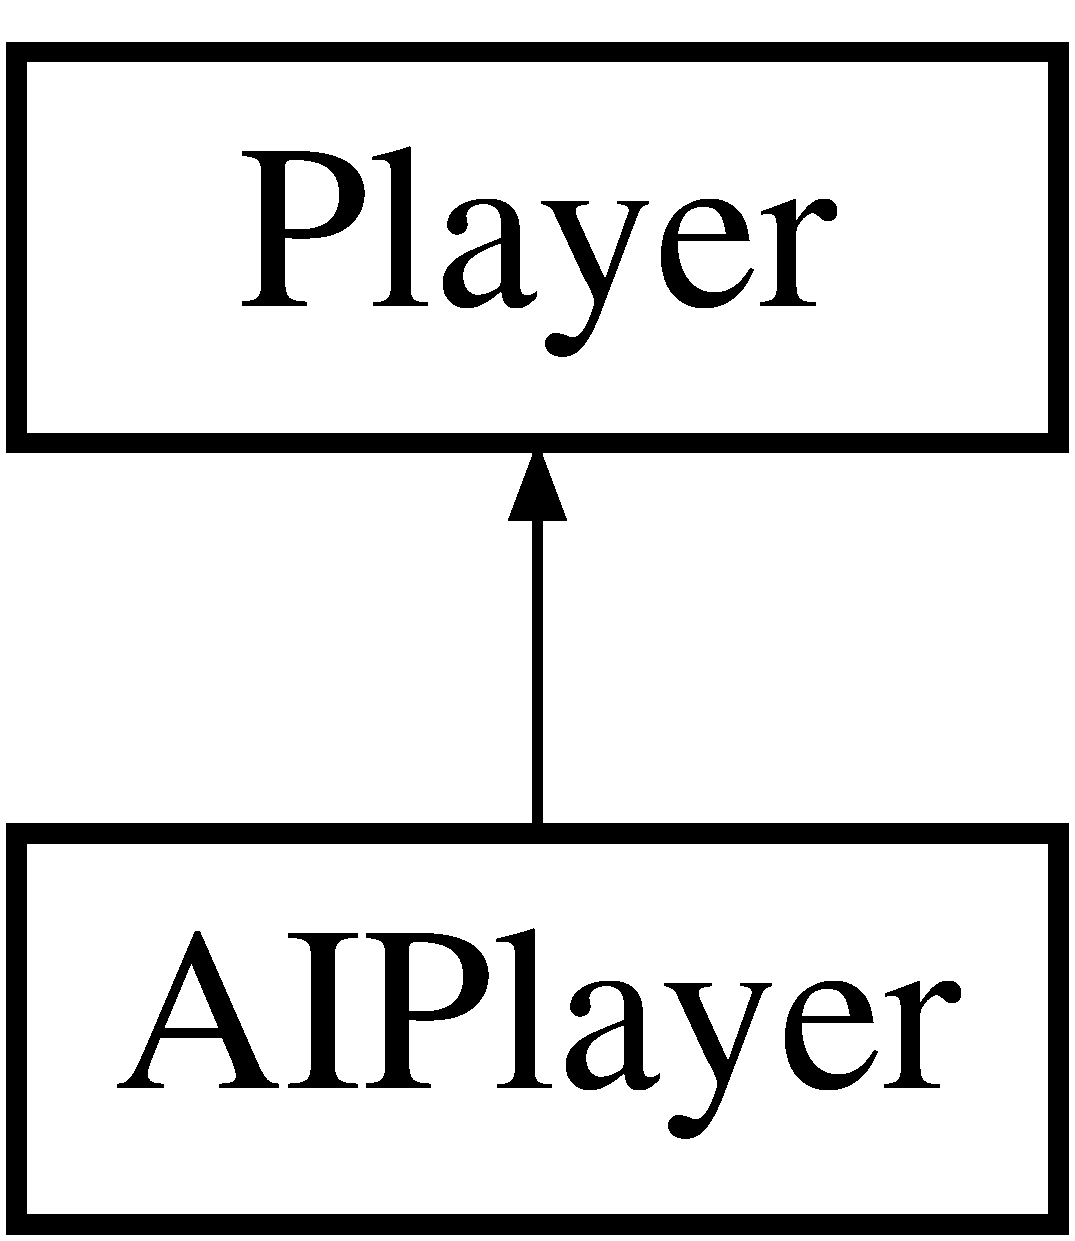
\includegraphics[height=2.000000cm]{class_a_i_player}
\end{center}
\end{figure}
\subsection*{Public Member Functions}
\begin{DoxyCompactItemize}
\item 
\hyperlink{class_a_i_player_af228dd97466ff5219f2e150935eb2565}{A\-I\-Player} (Q\-String s)
\item 
void \hyperlink{class_a_i_player_a6641fec98f51924a76ba00b4b3253325}{play} (\hyperlink{class_dictionary}{Dictionary} \&dict, \hyperlink{class_play}{Play} $\ast$$\ast$play)
\begin{DoxyCompactList}\small\item\em \hyperlink{class_a_i_player_a6641fec98f51924a76ba00b4b3253325}{A\-I\-Player\-::play} Fills the Currentplay of the board with a valid A\-I play. \end{DoxyCompactList}\item 
virtual bool \hyperlink{class_a_i_player_a2a71a31297386f4d69f12a43187954a6}{is\-A\-I\-Player} ()
\begin{DoxyCompactList}\small\item\em \hyperlink{class_a_i_player_a2a71a31297386f4d69f12a43187954a6}{A\-I\-Player\-::is\-A\-I\-Player}. \end{DoxyCompactList}\end{DoxyCompactItemize}
\subsection*{Private Member Functions}
\begin{DoxyCompactItemize}
\item 
size\-\_\-t \hyperlink{class_a_i_player_af50ad9f1d7a27e87ec67fe9ddb49ef93}{ai\-\_\-search} (Q\-List$<$ \hyperlink{class_letter}{Letter} $\ast$ $>$ $\ast$tiles, Q\-List$<$ \hyperlink{class_space}{Space} $\ast$ $>$ $\ast$positions, list$<$ \hyperlink{class_play}{Play} $\ast$ $>$ $\ast$playlist, \hyperlink{class_dictionary}{Dictionary} $\ast$dict)
\begin{DoxyCompactList}\small\item\em \hyperlink{class_a_i_player_af50ad9f1d7a27e87ec67fe9ddb49ef93}{A\-I\-Player\-::ai\-\_\-search} High level assistant function that creates a new position list we can tamper with. \end{DoxyCompactList}\item 
bool \hyperlink{class_a_i_player_a3bcac2df2a8f171dfedfa594855294af}{\-\_\-touches\-\_\-4} (int x, int y)
\begin{DoxyCompactList}\small\item\em \hyperlink{class_a_i_player_a3bcac2df2a8f171dfedfa594855294af}{A\-I\-Player\-::\-\_\-touches\-\_\-4} Returns whether or not there are spaces that contain Tiles around this location. \end{DoxyCompactList}\item 
bool \hyperlink{class_a_i_player_a158fb1339fc845f8b057d71b6e2f6381}{\-\_\-touches\-\_\-2} (int x, int y)
\begin{DoxyCompactList}\small\item\em \hyperlink{class_a_i_player_a158fb1339fc845f8b057d71b6e2f6381}{A\-I\-Player\-::\-\_\-touches\-\_\-2} Returns whether or not there are spaces that contain Tiles around this location. \end{DoxyCompactList}\item 
void \hyperlink{class_a_i_player_afdf893cf47209d106740f56c1d37c334}{\-\_\-assist\-\_\-ai\-\_\-search} (\hyperlink{class_trie_node}{Trie\-Node} $\ast$Node, Q\-List$<$ \hyperlink{class_letter}{Letter} $\ast$ $>$ $\ast$tiles, Q\-List$<$ \hyperlink{class_space}{Space} $\ast$ $>$ $\ast$positions, Q\-List$<$ \hyperlink{class_move}{Move} $\ast$ $>$ $\ast$playbuilder, list$<$ \hyperlink{class_play}{Play} $\ast$ $>$ $\ast$playlist)
\begin{DoxyCompactList}\small\item\em \hyperlink{class_a_i_player_afdf893cf47209d106740f56c1d37c334}{A\-I\-Player\-::\-\_\-assist\-\_\-ai\-\_\-search} This is the main function of the A\-I search, which tries to discover the various valid plays available. \end{DoxyCompactList}\end{DoxyCompactItemize}
\subsection*{Private Attributes}
\begin{DoxyCompactItemize}
\item 
\hyperlink{class_board}{Board} $\ast$ \hyperlink{class_a_i_player_a4262c0ef313e6ac9f3e5be3f2c4d6ade}{boardcopy}
\end{DoxyCompactItemize}
\subsection*{Additional Inherited Members}


\subsection{Detailed Description}


Definition at line 7 of file aiplayer.\-h.



\subsection{Constructor \& Destructor Documentation}
\hypertarget{class_a_i_player_af228dd97466ff5219f2e150935eb2565}{\index{A\-I\-Player@{A\-I\-Player}!A\-I\-Player@{A\-I\-Player}}
\index{A\-I\-Player@{A\-I\-Player}!AIPlayer@{A\-I\-Player}}
\subsubsection[{A\-I\-Player}]{\setlength{\rightskip}{0pt plus 5cm}A\-I\-Player\-::\-A\-I\-Player (
\begin{DoxyParamCaption}
\item[{Q\-String}]{s}
\end{DoxyParamCaption}
)\hspace{0.3cm}{\ttfamily [inline]}}}\label{class_a_i_player_af228dd97466ff5219f2e150935eb2565}


Definition at line 9 of file aiplayer.\-h.



Referenced by Dialog\-::setup\-Players().


\begin{DoxyCode}
9 : \hyperlink{class_player_ad079d0b82440f180a6698ff62f1dc1be}{Player}(s) \{\}
\end{DoxyCode}


\subsection{Member Function Documentation}
\hypertarget{class_a_i_player_afdf893cf47209d106740f56c1d37c334}{\index{A\-I\-Player@{A\-I\-Player}!\-\_\-assist\-\_\-ai\-\_\-search@{\-\_\-assist\-\_\-ai\-\_\-search}}
\index{\-\_\-assist\-\_\-ai\-\_\-search@{\-\_\-assist\-\_\-ai\-\_\-search}!AIPlayer@{A\-I\-Player}}
\subsubsection[{\-\_\-assist\-\_\-ai\-\_\-search}]{\setlength{\rightskip}{0pt plus 5cm}void A\-I\-Player\-::\-\_\-assist\-\_\-ai\-\_\-search (
\begin{DoxyParamCaption}
\item[{{\bf Trie\-Node} $\ast$}]{Node, }
\item[{Q\-List$<$ {\bf Letter} $\ast$ $>$ $\ast$}]{tiles, }
\item[{Q\-List$<$ {\bf Space} $\ast$ $>$ $\ast$}]{positions, }
\item[{Q\-List$<$ {\bf Move} $\ast$ $>$ $\ast$}]{playbuilder, }
\item[{list$<$ {\bf Play} $\ast$ $>$ $\ast$}]{playlist}
\end{DoxyParamCaption}
)\hspace{0.3cm}{\ttfamily [private]}}}\label{class_a_i_player_afdf893cf47209d106740f56c1d37c334}


\hyperlink{class_a_i_player_afdf893cf47209d106740f56c1d37c334}{A\-I\-Player\-::\-\_\-assist\-\_\-ai\-\_\-search} This is the main function of the A\-I search, which tries to discover the various valid plays available. 


\begin{DoxyParams}{Parameters}
{\em Node} & The current \hyperlink{class_trie_node}{Trie\-Node} representing the letter we are on during this search. \\
\hline
{\em tiles} & The remaining tiles in our tray to complete words with. \\
\hline
{\em positions} & The positions remaining in our searchgrid in this particular direction, on this particular line. \\
\hline
{\em playbuilder} & The unit that represents the play being built at the moment. \\
\hline
{\em playlist} & A location we edit to fill with valid plays -\/ and thus the 'return value' in a ways. \\
\hline
\end{DoxyParams}
\begin{DoxyRefDesc}{Todo}
\item[\hyperlink{todo__todo000001}{Todo}]Make it validate the full 'play' here before submitting it. If it doesn't validate, R\-E\-T\-U\-R\-N! Because we can't continue along this route to valid words anymore. It will never validate. We still have to do the position check after that either way. We can only do a sideways check however! Not a forwards, as that might invalidate a non-\/complete word that might complete later. \end{DoxyRefDesc}


Definition at line 55 of file aiplayer.\-cpp.



References \-\_\-touches\-\_\-4(), Letter\-::as\-Q\-Char\-Ptr(), Trie\-Node\-::find\-Child(), Rack\-::get\-Rack(), Space\-::get\-X(), Space\-::get\-Y(), Space\-::is\-Blank(), Trie\-Node\-::is\-Word(), and Space\-::letter.



Referenced by ai\-\_\-search().


\begin{DoxyCode}
57                                                         \{
58     \textcolor{keywordflow}{if}(!Node) \{
59         \textcolor{comment}{// This should never happen!}
60         cout << \textcolor{stringliteral}{"Big Error! Invalid control path!"};
61         \textcolor{keywordflow}{return};
62     \}
63 
64     \textcolor{keywordflow}{if}( Node->\hyperlink{class_trie_node_a3fa48afcb9376feaf24c9d8acac7c076}{isWord}() && !playbuilder->isEmpty() ) \{
65         \textcolor{keywordtype}{int} somethingtrue = \textcolor{keyword}{false};
66         \textcolor{keywordflow}{for}(\textcolor{keywordtype}{int} i = 0; i < playbuilder->size(); i++)
67         \{
68             \textcolor{keywordflow}{if}( \hyperlink{class_a_i_player_a3bcac2df2a8f171dfedfa594855294af}{\_touches\_4}(playbuilder->at(i)->getX(),
69                            playbuilder->at(i)->getY()) )
70                 somethingtrue = \textcolor{keyword}{true};
71         \}
72 
73         \textcolor{keywordflow}{if}( somethingtrue ) \{
82             \textcolor{keywordflow}{if}( !positions->isEmpty() ) \{
83                 \textcolor{keywordflow}{if}( positions->first()->letter == NULL ) \{
84                     \textcolor{comment}{// Add the play to the playlist}
85                     playlist->push\_front(\textcolor{keyword}{new} \hyperlink{class_play}{Play}(playbuilder,\textcolor{keyword}{this}));
86                 \}
87             \}
88             \textcolor{keywordflow}{else} \{
89                 \textcolor{comment}{// Add the play to the playlist}
90                 playlist->push\_front(\textcolor{keyword}{new} \hyperlink{class_play}{Play}(playbuilder,\textcolor{keyword}{this}));
91             \}
92         \}
93     \}
94 
95     \textcolor{comment}{// exit condition 1: If we have no tiles, we can't place letters.}
96     \textcolor{comment}{// exit condition 2: If we have no positions left to fill, we can't place letters.}
97     \textcolor{keywordflow}{if}( tiles->isEmpty() || positions->isEmpty() )
98         \textcolor{keywordflow}{return};
99 
100     \textcolor{comment}{// We are guaranteed to have a position letter, so we take it.}
101     \textcolor{comment}{// We are never going to give this space back.}
102     \textcolor{comment}{// (MC: Modification Character)}
103     \hyperlink{class_space}{Space}* mc = positions->takeFirst();
104     \textcolor{keywordtype}{int} tilepos = 0;
105 
106     \textcolor{comment}{// exit condition 3: if the position letter is not a wildcard,}
107     \textcolor{comment}{// we don't have to use a tile from our tray, and we instead just continue on}
108     \textcolor{comment}{// after we check that we have that child.}
109     \textcolor{keywordflow}{if}( mc->\hyperlink{class_space_a308f0ef400183df78df69717ca50cfee}{isBlank}() == false )
110     \{
111         \hyperlink{class_trie_node}{TrieNode} * foundchild = Node->\hyperlink{class_trie_node_a1b5c7d87ce28b9aa7d0bcbfe33868bbc}{findChild}(*mc->\hyperlink{class_space_ab899363fba4ab54c907df80a99e8e563}{letter}->
      \hyperlink{class_letter_aa7fb6547b5ceefef8d0a014ab0a80d08}{asQCharPtr}());
112         \textcolor{keywordflow}{if}( foundchild )
113             \hyperlink{class_a_i_player_afdf893cf47209d106740f56c1d37c334}{\_assist\_ai\_search}(foundchild,tiles,positions,playbuilder,playlist);
114     \}
115     \textcolor{keywordflow}{else}
116     \{
117         \textcolor{comment}{// We must now attempt this system for any character that is valid here.}
118         \textcolor{comment}{// It's luckily not 26, it's only as many tiles as we have available!}
119         \textcolor{comment}{// Still, in the WORST situation...}
120         \textcolor{comment}{// This means 7*6*5*4*3*2*1, or 7! total calls of recursion. That's 5040.}
121         \textcolor{comment}{// Also, we need to make sure it does get \_taken\_ by a letter.}
122 
123         \textcolor{keywordflow}{for}(tilepos = 0; tilepos < tiles->size(); tilepos++)
124         \{
125             \hyperlink{class_letter}{Letter} * t = tiles->takeAt(tilepos);
126 
127             \textcolor{comment}{// Take this letter and let's see if it can go somewhere.}
128             \textcolor{comment}{// Generate the current move.}
129 
130             \hyperlink{class_move}{Move} * mv = \textcolor{keyword}{new} \hyperlink{class_move}{Move}(\textcolor{keyword}{this}, t, \hyperlink{class_rack_aa48de650c15bda8267451d84caf6ea3f}{Rack::getRack}()->getPos(t), mc->
      \hyperlink{class_space_a65828dd5c8d2799dadab676c1d52bdfa}{getX}(), mc->\hyperlink{class_space_ac12e951586a96323b1db8cf1e5a827a9}{getY}());
131             playbuilder->push\_front(mv);
132 
133             \hyperlink{class_trie_node}{TrieNode} * foundchild = Node->\hyperlink{class_trie_node_a1b5c7d87ce28b9aa7d0bcbfe33868bbc}{findChild}(*(t->
      \hyperlink{class_letter_aa7fb6547b5ceefef8d0a014ab0a80d08}{asQCharPtr}()));
134             \textcolor{keywordflow}{if}( foundchild )
135             \{
136                 \hyperlink{class_a_i_player_afdf893cf47209d106740f56c1d37c334}{\_assist\_ai\_search}(foundchild,tiles,positions,playbuilder,playlist);
137             \}
138 
139             \textcolor{comment}{// And take it out of the playbuilder.}
140             playbuilder->pop\_front();
141             tiles->insert(tilepos,t);
142         \}
143     \}
144 \}
\end{DoxyCode}
\hypertarget{class_a_i_player_a158fb1339fc845f8b057d71b6e2f6381}{\index{A\-I\-Player@{A\-I\-Player}!\-\_\-touches\-\_\-2@{\-\_\-touches\-\_\-2}}
\index{\-\_\-touches\-\_\-2@{\-\_\-touches\-\_\-2}!AIPlayer@{A\-I\-Player}}
\subsubsection[{\-\_\-touches\-\_\-2}]{\setlength{\rightskip}{0pt plus 5cm}bool A\-I\-Player\-::\-\_\-touches\-\_\-2 (
\begin{DoxyParamCaption}
\item[{int}]{x, }
\item[{int}]{y}
\end{DoxyParamCaption}
)\hspace{0.3cm}{\ttfamily [private]}}}\label{class_a_i_player_a158fb1339fc845f8b057d71b6e2f6381}


\hyperlink{class_a_i_player_a158fb1339fc845f8b057d71b6e2f6381}{A\-I\-Player\-::\-\_\-touches\-\_\-2} Returns whether or not there are spaces that contain Tiles around this location. 


\begin{DoxyParams}{Parameters}
{\em x} & The location around which we want to look, in the {\itshape first} direction. \\
\hline
{\em y} & The location around which we want to look, in the {\itshape second} direction. \\
\hline
\end{DoxyParams}
\begin{DoxyReturn}{Returns}
bool true or false. 
\end{DoxyReturn}


Definition at line 28 of file aiplayer.\-cpp.



References Board\-::get\-Board(), Space\-::is\-Blank(), and Board\-::spaces.



Referenced by \-\_\-touches\-\_\-4(), and play().


\begin{DoxyCode}
28                                       \{
29     \hyperlink{class_board}{Board} * myboard = \hyperlink{class_board_ae30e802b1d83309fc95e695b5b3df338}{Board::getBoard}();
30     \textcolor{keywordflow}{if}( x+1 < 15) \{
31         \textcolor{keywordflow}{if}( !myboard->\hyperlink{class_board_a73b12248ddb6ee3adc24f4458d8661c2}{spaces}[x+1][y]->\hyperlink{class_space_a308f0ef400183df78df69717ca50cfee}{isBlank}() )
32             \textcolor{keywordflow}{return} \textcolor{keyword}{true};
33     \}
34     \textcolor{keywordflow}{if}( x-1 > 0) \{
35         \textcolor{keywordflow}{if}( !myboard->\hyperlink{class_board_a73b12248ddb6ee3adc24f4458d8661c2}{spaces}[x-1][y]->\hyperlink{class_space_a308f0ef400183df78df69717ca50cfee}{isBlank}() )
36             \textcolor{keywordflow}{return} \textcolor{keyword}{true};
37     \}
38     \textcolor{comment}{// Fall-through logic. If it reaches here, then all of the previous items would have 'returned false'.}
39     \textcolor{keywordflow}{return} \textcolor{keyword}{false};
40 \}
\end{DoxyCode}
\hypertarget{class_a_i_player_a3bcac2df2a8f171dfedfa594855294af}{\index{A\-I\-Player@{A\-I\-Player}!\-\_\-touches\-\_\-4@{\-\_\-touches\-\_\-4}}
\index{\-\_\-touches\-\_\-4@{\-\_\-touches\-\_\-4}!AIPlayer@{A\-I\-Player}}
\subsubsection[{\-\_\-touches\-\_\-4}]{\setlength{\rightskip}{0pt plus 5cm}bool A\-I\-Player\-::\-\_\-touches\-\_\-4 (
\begin{DoxyParamCaption}
\item[{int}]{x, }
\item[{int}]{y}
\end{DoxyParamCaption}
)\hspace{0.3cm}{\ttfamily [private]}}}\label{class_a_i_player_a3bcac2df2a8f171dfedfa594855294af}


\hyperlink{class_a_i_player_a3bcac2df2a8f171dfedfa594855294af}{A\-I\-Player\-::\-\_\-touches\-\_\-4} Returns whether or not there are spaces that contain Tiles around this location. 


\begin{DoxyParams}{Parameters}
{\em x} & The location around which we want to look, in the x direction. \\
\hline
{\em y} & The location around which we want to look, in the y direction. \\
\hline
\end{DoxyParams}
\begin{DoxyReturn}{Returns}
bool true or false. 
\end{DoxyReturn}


Definition at line 11 of file aiplayer.\-cpp.



References \-\_\-touches\-\_\-2(), and Board\-::get\-Board().



Referenced by \-\_\-assist\-\_\-ai\-\_\-search().


\begin{DoxyCode}
11                                       \{
12     \textcolor{keywordflow}{if}(!\hyperlink{class_board_ae30e802b1d83309fc95e695b5b3df338}{Board::getBoard}()->startCovered())
13         \textcolor{keywordflow}{return} \textcolor{keyword}{true};
14     \textcolor{keywordflow}{if}(\hyperlink{class_a_i_player_a158fb1339fc845f8b057d71b6e2f6381}{\_touches\_2}(x,y))
15         \textcolor{keywordflow}{return} \textcolor{keyword}{true};
16     \textcolor{keywordflow}{else} \textcolor{keywordflow}{if}(\hyperlink{class_a_i_player_a158fb1339fc845f8b057d71b6e2f6381}{\_touches\_2}(y,x))
17         \textcolor{keywordflow}{return} \textcolor{keyword}{true};
18     \textcolor{comment}{// Fall-through logic. If it reaches here, then all of the previous items would have 'returned false'.}
19     \textcolor{keywordflow}{return} \textcolor{keyword}{false};
20 \}
\end{DoxyCode}
\hypertarget{class_a_i_player_af50ad9f1d7a27e87ec67fe9ddb49ef93}{\index{A\-I\-Player@{A\-I\-Player}!ai\-\_\-search@{ai\-\_\-search}}
\index{ai\-\_\-search@{ai\-\_\-search}!AIPlayer@{A\-I\-Player}}
\subsubsection[{ai\-\_\-search}]{\setlength{\rightskip}{0pt plus 5cm}size\-\_\-t A\-I\-Player\-::ai\-\_\-search (
\begin{DoxyParamCaption}
\item[{Q\-List$<$ {\bf Letter} $\ast$ $>$ $\ast$}]{tiles, }
\item[{Q\-List$<$ {\bf Space} $\ast$ $>$ $\ast$}]{positions, }
\item[{list$<$ {\bf Play} $\ast$ $>$ $\ast$}]{playlist, }
\item[{{\bf Dictionary} $\ast$}]{dict}
\end{DoxyParamCaption}
)\hspace{0.3cm}{\ttfamily [private]}}}\label{class_a_i_player_af50ad9f1d7a27e87ec67fe9ddb49ef93}


\hyperlink{class_a_i_player_af50ad9f1d7a27e87ec67fe9ddb49ef93}{A\-I\-Player\-::ai\-\_\-search} High level assistant function that creates a new position list we can tamper with. 


\begin{DoxyParams}{Parameters}
{\em tiles} & The tiles we have available to us. Because this is a pointer, this function can not be parallelized at this time. Guaranteed to restore the tiles to their correct state when finished. \\
\hline
{\em positions} & The original positions we want to search through. \\
\hline
{\em playlist} & The current list of plays we can do. Constructive. \\
\hline
{\em dict} & The dictionary we will be grabbed the node out of. \\
\hline
\end{DoxyParams}
\begin{DoxyReturn}{Returns}
The quantity if plays available to the A\-I after this function finishes. 
\end{DoxyReturn}


Definition at line 155 of file aiplayer.\-cpp.



References \-\_\-assist\-\_\-ai\-\_\-search(), Trie\-::root, and Dictionary\-::words.



Referenced by play().


\begin{DoxyCode}
157 \{
158     QList<Space*> * pos\_copy = \textcolor{keyword}{new} QList<Space*>();
159 
160     \textcolor{keywordflow}{for}(\textcolor{keywordtype}{int} i = 0; i < positions->size(); i++) \{
161         pos\_copy->insert(i,positions->at(i));
162     \}
163 
164     \textcolor{keywordflow}{if}(dict->\hyperlink{class_dictionary_ac6c08127a37d8131fb8fb1e738406e85}{words}->\hyperlink{class_trie_a052cecab75ca88758778d340ed002d66}{root})
165         \hyperlink{class_a_i_player_afdf893cf47209d106740f56c1d37c334}{\_assist\_ai\_search}(dict->\hyperlink{class_dictionary_ac6c08127a37d8131fb8fb1e738406e85}{words}->\hyperlink{class_trie_a052cecab75ca88758778d340ed002d66}{root}, tiles, pos\_copy, \textcolor{keyword}{new} QList<Move*>(),
       playlist);
166     \textcolor{keywordflow}{return} playlist->size();
167 \}
\end{DoxyCode}
\hypertarget{class_a_i_player_a2a71a31297386f4d69f12a43187954a6}{\index{A\-I\-Player@{A\-I\-Player}!is\-A\-I\-Player@{is\-A\-I\-Player}}
\index{is\-A\-I\-Player@{is\-A\-I\-Player}!AIPlayer@{A\-I\-Player}}
\subsubsection[{is\-A\-I\-Player}]{\setlength{\rightskip}{0pt plus 5cm}bool A\-I\-Player\-::is\-A\-I\-Player (
\begin{DoxyParamCaption}
{}
\end{DoxyParamCaption}
)\hspace{0.3cm}{\ttfamily [virtual]}}}\label{class_a_i_player_a2a71a31297386f4d69f12a43187954a6}


\hyperlink{class_a_i_player_a2a71a31297386f4d69f12a43187954a6}{A\-I\-Player\-::is\-A\-I\-Player}. 

This is an overloaded member function, provided for convenience. It differs from the above function only in what argument(s) it accepts. \begin{DoxyReturn}{Returns}
True if player is A\-I 
\end{DoxyReturn}


Reimplemented from \hyperlink{class_player_afcd43a9498dc70a71ba17484699446bb}{Player}.



Definition at line 370 of file aiplayer.\-cpp.


\begin{DoxyCode}
370                          \{
371     \textcolor{keywordflow}{return} \textcolor{keyword}{true};
372 \}
\end{DoxyCode}
\hypertarget{class_a_i_player_a6641fec98f51924a76ba00b4b3253325}{\index{A\-I\-Player@{A\-I\-Player}!play@{play}}
\index{play@{play}!AIPlayer@{A\-I\-Player}}
\subsubsection[{play}]{\setlength{\rightskip}{0pt plus 5cm}void A\-I\-Player\-::play (
\begin{DoxyParamCaption}
\item[{{\bf Dictionary} \&}]{dict, }
\item[{{\bf Play} $\ast$$\ast$}]{play}
\end{DoxyParamCaption}
)}}\label{class_a_i_player_a6641fec98f51924a76ba00b4b3253325}


\hyperlink{class_a_i_player_a6641fec98f51924a76ba00b4b3253325}{A\-I\-Player\-::play} Fills the Currentplay of the board with a valid A\-I play. 


\begin{DoxyParams}{Parameters}
{\em dict} & The dictionary we want to use as a reference to form a valid play. \\
\hline
{\em play} & The play we will be editing. Pointer to 'currentplay' on the board. \\
\hline
\end{DoxyParams}


Definition at line 174 of file aiplayer.\-cpp.



References \-\_\-pred\-\_\-value\-\_\-sort(), \-\_\-touches\-\_\-2(), ai\-\_\-search(), boardcopy, Space\-::clear(), Play\-::clear\-Letter(), Board\-::get\-Board(), Move\-::get\-Letter(), Rack\-::get\-Rack(), Move\-::get\-Rack\-Position(), Move\-::get\-X(), Move\-::get\-Y(), Rack\-::inactivate\-By\-Letter(), Space\-::is\-Blank(), Player\-::letters, Board\-::move\-Letter\-To\-Board(), Play\-::moves, Space\-::set\-New(), Board\-::spaces, Board\-::start\-Covered(), and Board\-::validate().


\begin{DoxyCode}
174                                                 \{
175     \textcolor{keywordtype}{int} searches = 0;
176 
177     \hyperlink{class_board}{Board} * myboard = this->\hyperlink{class_a_i_player_a4262c0ef313e6ac9f3e5be3f2c4d6ade}{boardcopy} = \hyperlink{class_board_ae30e802b1d83309fc95e695b5b3df338}{Board::getBoard}();
178     list<Play*> * possible\_plays = \textcolor{keyword}{new} list<Play*>();
179 
180     assert(this->\hyperlink{class_player_abd40dc8f6d524bd1331a8133e9bb8902}{letters}.size());
181     \textcolor{comment}{/* Putting the letters into a prefered format */}
182     QVector<Letter*> myletterv = QVector<Letter*>::fromStdVector(this->\hyperlink{class_player_abd40dc8f6d524bd1331a8133e9bb8902}{letters});
183     QList<Letter*> myletters\_ll = QList<Letter*>::fromVector(myletterv);
184     QList<Letter*> * myletters = &myletters\_ll;
185 
186     \textcolor{comment}{/* Prepare the anchor characters. */}
187     QList<Space *> * rightanchors[15];
188     QList<Space *> * downanchors[15];
189 
190     \textcolor{keywordflow}{for}( \textcolor{keywordtype}{int} i = 0; i<15; i++)
191     \{
192         rightanchors[i] = \textcolor{keyword}{new} QList<Space *>();
193         downanchors[i] = \textcolor{keyword}{new} QList<Space *>();
194     \}
195 
196     \textcolor{comment}{// First, we find out if this is the initial play. As in, we can play 'anything'.}
197     \textcolor{comment}{// Thus, this is the only anchor we need, and we set it as such.}
198     \textcolor{keywordflow}{if} ( \hyperlink{class_board_ae30e802b1d83309fc95e695b5b3df338}{Board::getBoard}()->\hyperlink{class_board_a4a04a6fc41d20c9836b23826dc7f6026}{startCovered}() == false )
199     \{
200         \textcolor{keywordflow}{for}(\textcolor{keywordtype}{int} i = 0; i < 15; i++)
201             rightanchors[0]->push\_back(myboard->\hyperlink{class_board_a73b12248ddb6ee3adc24f4458d8661c2}{spaces}[i][7]);
202     \}
203     \textcolor{comment}{// Otherwise, we need to go through the entire board and collect anchoring lines.}
204     \textcolor{comment}{// We need an array of each horizontal, and an array of each vertical line.}
205     \textcolor{comment}{// Any line that has no elements in it, gets cleared. This way, we save processor power.}
206     \textcolor{comment}{// Thanks to this system being 2d and a perfect square, we can stick these two into the same}
207     \textcolor{comment}{// double loop.}
208     \textcolor{keywordflow}{else} \{
209         \textcolor{keywordflow}{for}(\textcolor{keywordtype}{int} i = 0; i<15; i++)
210         \{
211             \textcolor{keywordtype}{bool} isempty\_r = \textcolor{keyword}{true};
212             \textcolor{keywordtype}{bool} isempty\_d = \textcolor{keyword}{true};
213 
214             \textcolor{keywordflow}{for}(\textcolor{keywordtype}{int} j = 0; j<15; j++) \{
215                 \textcolor{keywordflow}{if}(myboard->\hyperlink{class_board_a73b12248ddb6ee3adc24f4458d8661c2}{spaces}[i][j]->\hyperlink{class_space_a308f0ef400183df78df69717ca50cfee}{isBlank}() == \textcolor{keyword}{false} || 
      \hyperlink{class_a_i_player_a158fb1339fc845f8b057d71b6e2f6381}{\_touches\_2}(i,j) )
216                     isempty\_r = \textcolor{keyword}{false};
217                 \textcolor{keywordflow}{if}(myboard->\hyperlink{class_board_a73b12248ddb6ee3adc24f4458d8661c2}{spaces}[j][i]->\hyperlink{class_space_a308f0ef400183df78df69717ca50cfee}{isBlank}() == \textcolor{keyword}{false} || 
      \hyperlink{class_a_i_player_a158fb1339fc845f8b057d71b6e2f6381}{\_touches\_2}(j,i) )
218                     isempty\_d = \textcolor{keyword}{false};
219 
220                 rightanchors[i]->insert(j,myboard->\hyperlink{class_board_a73b12248ddb6ee3adc24f4458d8661c2}{spaces}[i][j]);
221                 downanchors[i]->insert(j,myboard->\hyperlink{class_board_a73b12248ddb6ee3adc24f4458d8661c2}{spaces}[j][i]);
222             \}
223 
224             \textcolor{keywordflow}{if}(isempty\_r)
225                 rightanchors[i]->clear();
226             \textcolor{keywordflow}{if}(isempty\_d)
227                 downanchors[i]->clear();
228         \}
229     \}
230 
231     \textcolor{comment}{/*}
232 \textcolor{comment}{     * Based on the anchors, we'll need to do this multiple times, downwards and rightwards}
233 \textcolor{comment}{     * But we can ignore things that are 'part' of a word. It's already a word, and we can't}
234 \textcolor{comment}{     * continue any better from it, than when we were at the start of that word.}
235 \textcolor{comment}{     */}
236     \textcolor{keywordflow}{for}(\textcolor{keywordtype}{int} i = 0; i < 15; i++)
237     \{
238         \textcolor{keywordtype}{bool} anchoring\_r = \textcolor{keyword}{false};
239         \textcolor{keywordtype}{bool} anchoring\_d = \textcolor{keyword}{false};
240 
241         \textcolor{comment}{// We can't create a word if a line is empty!}
242         \textcolor{keywordflow}{if}(!rightanchors[i]->isEmpty()) \{
243             \textcolor{keywordflow}{for}( \textcolor{keywordtype}{int} j = 0; j < 15; j++) \{
244                 \textcolor{comment}{// Going Right}
245                 \textcolor{keywordflow}{if}( myboard->\hyperlink{class_board_a73b12248ddb6ee3adc24f4458d8661c2}{spaces}[i][j]->\hyperlink{class_space_a308f0ef400183df78df69717ca50cfee}{isBlank}() ) \{
246                     anchoring\_r = \textcolor{keyword}{false};
247                     \hyperlink{class_a_i_player_af50ad9f1d7a27e87ec67fe9ddb49ef93}{ai\_search}(myletters, rightanchors[i],possible\_plays,&dict);
248                     searches++;
249                 \}
250                 \textcolor{keywordflow}{else} \textcolor{keywordflow}{if}( !anchoring\_r ) \{
251                     anchoring\_r = \textcolor{keyword}{true};
252                     \hyperlink{class_a_i_player_af50ad9f1d7a27e87ec67fe9ddb49ef93}{ai\_search}(myletters, rightanchors[i],possible\_plays,&dict);
253                     searches++;
254                 \}
255                 \textcolor{comment}{// Otherwise, we are looking at a word, and we just pop.}
256                 \textcolor{comment}{// No need to do a search, because our last search was already good for this.}
257                 \textcolor{keywordflow}{if}(!rightanchors[i]->isEmpty()) \textcolor{comment}{// Safety for some reason.}
258                     rightanchors[i]->pop\_front();
259             \}
260         \}
261 
262         \textcolor{comment}{// We can't create a word if a line is empty!}
263         \textcolor{keywordflow}{if}(!downanchors[i]->isEmpty())
264         \{
265             \textcolor{keywordflow}{for}( \textcolor{keywordtype}{int} j = 0; j < 15; j++) \{
266                 \textcolor{comment}{// Going Down}
267                 \textcolor{keywordflow}{if}( myboard->\hyperlink{class_board_a73b12248ddb6ee3adc24f4458d8661c2}{spaces}[j][i]->\hyperlink{class_space_a308f0ef400183df78df69717ca50cfee}{isBlank}() ) \{
268                     anchoring\_d = \textcolor{keyword}{false};
269                     \hyperlink{class_a_i_player_af50ad9f1d7a27e87ec67fe9ddb49ef93}{ai\_search}(myletters, downanchors[i],possible\_plays,&dict);
270                     searches++;
271                 \}
272                 \textcolor{keywordflow}{else} \textcolor{keywordflow}{if}( !anchoring\_d ) \{
273                     anchoring\_d = \textcolor{keyword}{true};
274                     \hyperlink{class_a_i_player_af50ad9f1d7a27e87ec67fe9ddb49ef93}{ai\_search}(myletters, downanchors[i],possible\_plays,&dict);
275                     searches++;
276                 \}
277 
278                 \textcolor{comment}{// Otherwise, we are looking at a word, and we just pop.}
279                 \textcolor{comment}{// No need to do a search, because our last search was already good for this.}
280                 \textcolor{keywordflow}{if}(!downanchors[i]->isEmpty()) \textcolor{comment}{// Safety for some reason.}
281                     downanchors[i]->pop\_front();
282             \}
283         \}
284     \}
285 
286     \textcolor{comment}{/* make decision logic based on the values of these possible plays}
287 \textcolor{comment}{     * preferably by sorting the players in the possible plays.}
288 \textcolor{comment}{     */}
289     cout << \textcolor{stringliteral}{"We have generated "} << possible\_plays->size() << \textcolor{stringliteral}{" Qplays after "}
290          << searches << \textcolor{stringliteral}{" searches."} << endl;
291 
292 
293     possible\_plays->sort(\hyperlink{aiplayer_8cpp_a5ec041e0f53c78a5b4267c3df32ee188}{\_pred\_value\_sort});
294 
295 
296     \textcolor{comment}{/*}
297 \textcolor{comment}{     *  Purely debug output going on here.}
298 \textcolor{comment}{     */}
299     \textcolor{comment}{/*}
300 \textcolor{comment}{    int i = 0;}
301 \textcolor{comment}{    for(list<Play*>::const\_iterator it = possible\_plays->cbegin(); it != possible\_plays->cend(); it++)}
302 \textcolor{comment}{    \{}
303 \textcolor{comment}{        Play * c = *it;}
304 \textcolor{comment}{        cout << "Play Number " << i << ":";}
305 \textcolor{comment}{        string word = "";}
306 \textcolor{comment}{        // for( int j = 0; j < newlist.at(i)->size(); j++)}
307 \textcolor{comment}{}
308 \textcolor{comment}{        for(QList<Move*>::ConstIterator moveit = c->moves->cbegin(); moveit != c->moves->cend(); moveit++)}
309 \textcolor{comment}{        \{}
310 \textcolor{comment}{            Move * cur = *moveit;}
311 \textcolor{comment}{            cout << cur->getLetter()->asQCharPtr()->toLatin1();}
312 \textcolor{comment}{            cout << "@[" << cur->getX() << "][" << cur->getY() << "] ";}
313 \textcolor{comment}{            // word += *cur->getLetter()->asQCharPtr();}
314 \textcolor{comment}{            word += cur->getLetter()->asQCharPtr()->toLatin1();}
315 \textcolor{comment}{            cout << "@RP" << cur->getRackPosition() << "   ";}
316 \textcolor{comment}{        \}}
317 \textcolor{comment}{}
318 \textcolor{comment}{        cout << " ::: " << word << " == " << c->getCharArray().toStdString();}
319 \textcolor{comment}{        cout << " with value: " << c->getValue();}
320 \textcolor{comment}{        cout << endl;}
321 \textcolor{comment}{}
322 \textcolor{comment}{}
323 \textcolor{comment}{        i++;}
324 \textcolor{comment}{    \}}
325 \textcolor{comment}{    */}
326 
327     \textcolor{keywordflow}{if}(possible\_plays->empty() == \textcolor{keyword}{false})
328     \{
329         \hyperlink{class_play}{Play} * curplay = possible\_plays->front();
330         \textcolor{keywordtype}{bool} hasvalidplay = \textcolor{keyword}{false};
331 
332         \textcolor{keywordflow}{for}( QList<Move*>::Iterator moveit = curplay->\hyperlink{class_play_ade35ae53bff24e1755a935899ee018ed}{moves}->begin(); moveit != curplay->
      \hyperlink{class_play_ade35ae53bff24e1755a935899ee018ed}{moves}->end(); moveit++)
333         \{
334             \hyperlink{class_move}{Move} * curmove = *moveit;
335             myboard->\hyperlink{class_board_a8ed329bcdb775a910a575161ee5221ac}{moveLetterToBoard}(curmove->\hyperlink{class_move_ad78bb76d9b590cdb98aa4d4a3088e69d}{getRackPosition}(),curmove->
      \hyperlink{class_move_a7e3169f48fcca1aa1de4a5cbe67a284d}{getX}(),curmove->\hyperlink{class_move_af388d15d91f61a1f909998f50988ac1a}{getY}());
336         \}
337 
338         \textcolor{keywordflow}{for}( list<Play*>::const\_iterator it = possible\_plays->begin(); it != possible\_plays->end() && !(
      hasvalidplay = myboard->\hyperlink{class_board_a6f71df81a77438867e79f956afedb141}{validate}()); it++)
339         \{
340             \textcolor{comment}{// Our last play was invalid. So pick them back off of the board and clear the CurrentPlay.}
341             ((\hyperlink{class_play}{Play}*)*play)->clearMoves();
342             \textcolor{keywordflow}{for}( QList<Move*>::ConstIterator moveit = curplay->\hyperlink{class_play_ade35ae53bff24e1755a935899ee018ed}{moves}->cbegin(); moveit != curplay->
      \hyperlink{class_play_ade35ae53bff24e1755a935899ee018ed}{moves}->cend(); moveit++)
343             \{
344                 \hyperlink{class_move}{Move} * curmove = *moveit;
345                 myboard->\hyperlink{class_board_a73b12248ddb6ee3adc24f4458d8661c2}{spaces}[curmove->\hyperlink{class_move_a7e3169f48fcca1aa1de4a5cbe67a284d}{getX}()][curmove->\hyperlink{class_move_af388d15d91f61a1f909998f50988ac1a}{getY}()]->
      \hyperlink{class_space_a3afac453f54e569a94164c41a9721643}{setNew}();
346                 curplay->\hyperlink{class_play_a034c9cc986629045cdfcdbdeaabb2ab4}{clearLetter}(curmove->\hyperlink{class_move_a0c29654c98269d65c6af694eb441d382}{getLetter}());
347                 \hyperlink{class_rack_aa48de650c15bda8267451d84caf6ea3f}{Rack::getRack}()->\hyperlink{class_rack_afdf845eb458b07ed6029d29672ab120f}{inactivateByLetter}(curmove->
      \hyperlink{class_move_a0c29654c98269d65c6af694eb441d382}{getLetter}());
348                 myboard->\hyperlink{class_board_a73b12248ddb6ee3adc24f4458d8661c2}{spaces}[curmove->\hyperlink{class_move_a7e3169f48fcca1aa1de4a5cbe67a284d}{getX}()][curmove->\hyperlink{class_move_af388d15d91f61a1f909998f50988ac1a}{getY}()]->
      \hyperlink{class_space_ab18791c1da302a91c51477108be478b5}{clear}();
349             \}
350 
351             curplay = *it;
352             \textcolor{comment}{// cout << ">>" << curplay->getCharArray().toStdString() << "<<" << endl;}
353 
354             \textcolor{keywordflow}{for}( QList<Move*>::ConstIterator moveit = curplay->\hyperlink{class_play_ade35ae53bff24e1755a935899ee018ed}{moves}->cbegin(); moveit != curplay->
      \hyperlink{class_play_ade35ae53bff24e1755a935899ee018ed}{moves}->cend(); moveit++)
355             \{
356                 \hyperlink{class_move}{Move} * curmove = *moveit;
357                 myboard->\hyperlink{class_board_a8ed329bcdb775a910a575161ee5221ac}{moveLetterToBoard}(curmove->
      \hyperlink{class_move_ad78bb76d9b590cdb98aa4d4a3088e69d}{getRackPosition}(),curmove->\hyperlink{class_move_a7e3169f48fcca1aa1de4a5cbe67a284d}{getX}(),curmove->\hyperlink{class_move_af388d15d91f61a1f909998f50988ac1a}{getY}());
358             \}
359 
360             \textcolor{comment}{//cout << *Board::getBoard() << endl;}
361         \}
362     \}
363 \}
\end{DoxyCode}


\subsection{Member Data Documentation}
\hypertarget{class_a_i_player_a4262c0ef313e6ac9f3e5be3f2c4d6ade}{\index{A\-I\-Player@{A\-I\-Player}!boardcopy@{boardcopy}}
\index{boardcopy@{boardcopy}!AIPlayer@{A\-I\-Player}}
\subsubsection[{boardcopy}]{\setlength{\rightskip}{0pt plus 5cm}{\bf Board}$\ast$ A\-I\-Player\-::boardcopy\hspace{0.3cm}{\ttfamily [private]}}}\label{class_a_i_player_a4262c0ef313e6ac9f3e5be3f2c4d6ade}


Definition at line 28 of file aiplayer.\-h.



Referenced by play().



The documentation for this class was generated from the following files\-:\begin{DoxyCompactItemize}
\item 
Scrabble/\hyperlink{aiplayer_8h}{aiplayer.\-h}\item 
Scrabble/\hyperlink{aiplayer_8cpp}{aiplayer.\-cpp}\end{DoxyCompactItemize}

\hypertarget{class_board}{\section{Board Class Reference}
\label{class_board}\index{Board@{Board}}
}


The \hyperlink{class_board}{Board} class Singleton that represents a playing board.  




{\ttfamily \#include $<$board.\-h$>$}

Inheritance diagram for Board\-:\begin{figure}[H]
\begin{center}
\leavevmode
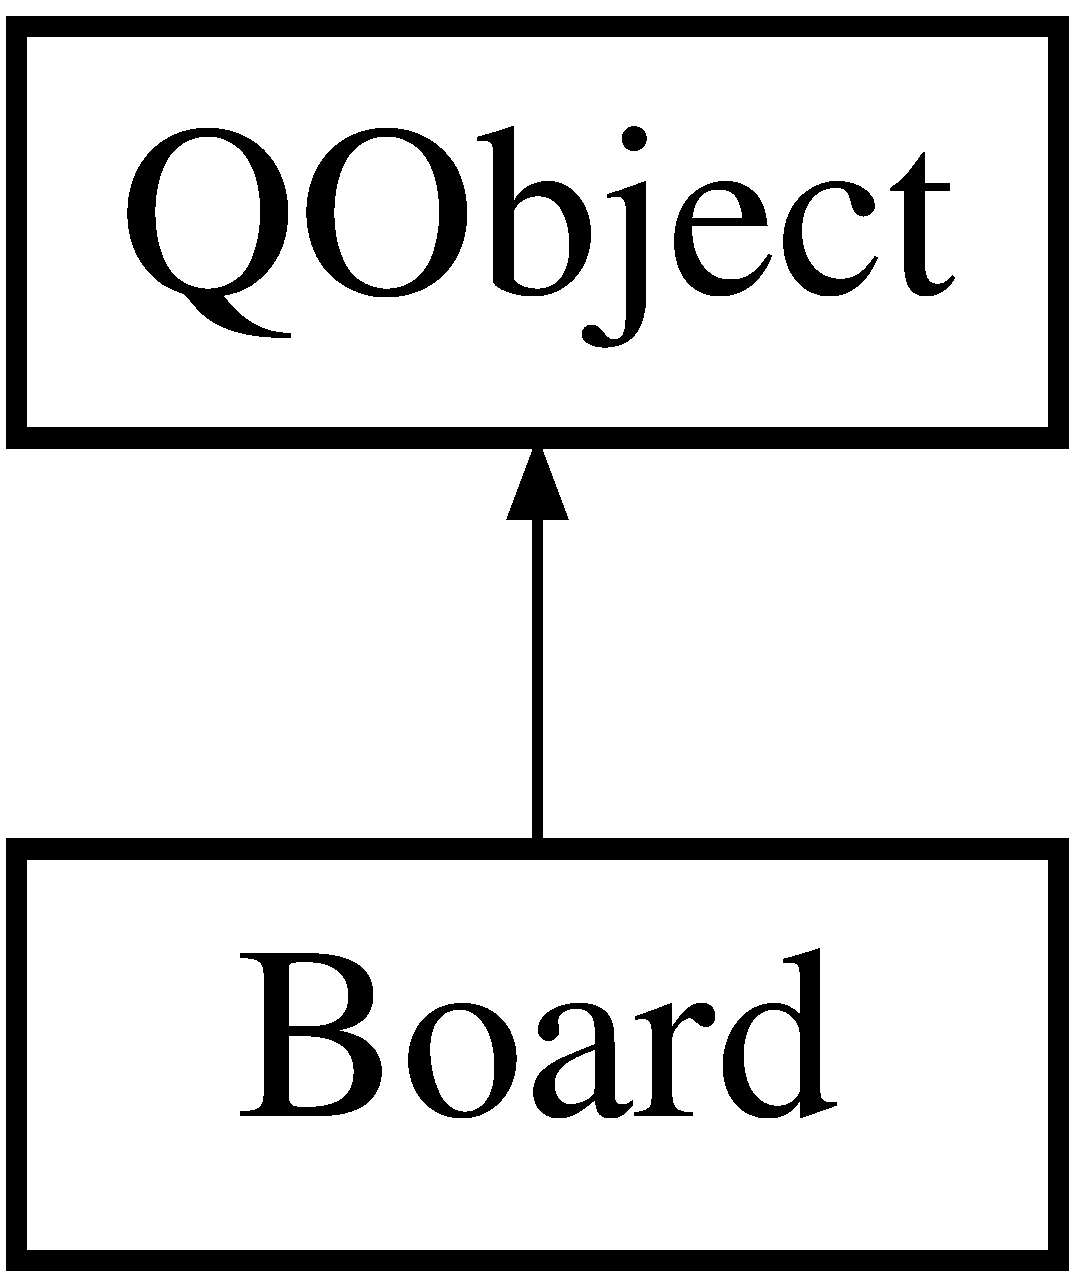
\includegraphics[height=2.000000cm]{class_board}
\end{center}
\end{figure}
\subsection*{Public Slots}
\begin{DoxyCompactItemize}
\item 
void \hyperlink{class_board_a9811fc5a0ae0953a45ff7e576af9411d}{on\-\_\-cancel\-Button\-\_\-clicked} ()
\begin{DoxyCompactList}\small\item\em \hyperlink{class_board_a9811fc5a0ae0953a45ff7e576af9411d}{Board\-::on\-\_\-cancel\-Button\-\_\-clicked} Cancels a play. Removes all letters from the board and resets the rack. \end{DoxyCompactList}\item 
void \hyperlink{class_board_a6aed1991c2174d60b320545db8ea015d}{on\-\_\-pass\-Button\-\_\-clicked} ()
\begin{DoxyCompactList}\small\item\em \hyperlink{class_board_a6aed1991c2174d60b320545db8ea015d}{Board\-::on\-\_\-pass\-Button\-\_\-clicked} Passes a players turn. \end{DoxyCompactList}\item 
void \hyperlink{class_board_afacf11c194d187ece00a84aa2504ca31}{on\-\_\-play\-Button\-\_\-clicked} ()
\begin{DoxyCompactList}\small\item\em \hyperlink{class_board_afacf11c194d187ece00a84aa2504ca31}{Board\-::on\-\_\-play\-Button\-\_\-clicked} Commits a play to the board if valid, or removes all pieces if not. \end{DoxyCompactList}\end{DoxyCompactItemize}
\subsection*{Signals}
\begin{DoxyCompactItemize}
\item 
void \hyperlink{class_board_a4149ab29681bf6745ef51e18a389aad3}{board\-Clicked} (int, int)
\item 
void \hyperlink{class_board_a8333b50e98ce792ebd3afe551751ce56}{invalid\-Move} ()
\end{DoxyCompactItemize}
\subsection*{Public Member Functions}
\begin{DoxyCompactItemize}
\item 
\hyperlink{class_board_af73f45730119a1fd8f6670f53f959e68}{$\sim$\-Board} ()
\begin{DoxyCompactList}\small\item\em \hyperlink{class_board_af73f45730119a1fd8f6670f53f959e68}{Board\-::$\sim$\-Board} Destructor. \end{DoxyCompactList}\item 
\hyperlink{class_board}{Board} $\ast$ \hyperlink{class_board_a13c88b0bc7d2a85f7e53790e71bdd403}{reset} ()
\begin{DoxyCompactList}\small\item\em \hyperlink{class_board_a13c88b0bc7d2a85f7e53790e71bdd403}{Board\-::reset} Resets the board by clearing out all the spaces. \end{DoxyCompactList}\item 
\hyperlink{class_board}{Board} $\ast$ \hyperlink{class_board_ae08098fe478e2832e7e7403140314164}{set\-Game} (\hyperlink{class_game}{Game} $\ast$)
\begin{DoxyCompactList}\small\item\em \hyperlink{class_board_ae08098fe478e2832e7e7403140314164}{Board\-::set\-Game} Setter for game. \end{DoxyCompactList}\item 
\hyperlink{class_game}{Game} $\ast$ \hyperlink{class_board_af09f0761a753008aa12021986ad6bc52}{get\-Game} ()
\begin{DoxyCompactList}\small\item\em \hyperlink{class_board_af09f0761a753008aa12021986ad6bc52}{Board\-::get\-Game} Gets a game. \end{DoxyCompactList}\item 
\hyperlink{class_board}{Board} $\ast$ \hyperlink{class_board_a43514bd0ab816eaed9affaace84686fe}{setup} ()
\begin{DoxyCompactList}\small\item\em \hyperlink{class_board_a43514bd0ab816eaed9affaace84686fe}{Board\-::setup} Sets up the board. \end{DoxyCompactList}\item 
\hyperlink{class_board}{Board} $\ast$ \hyperlink{class_board_a61a3bf8888e7969e3b34d7df279b495d}{inactivate\-Other\-Spaces} (int, int)
\begin{DoxyCompactList}\small\item\em \hyperlink{class_board_a61a3bf8888e7969e3b34d7df279b495d}{Board\-::inactivate\-Other\-Spaces} Inactivates other spaces on the board. \end{DoxyCompactList}\item 
int \hyperlink{class_board_a48c3a272cb4a47509ddd88edaec2bb59}{score} (\hyperlink{class_play}{Play} $\ast$)
\begin{DoxyCompactList}\small\item\em \hyperlink{class_board_a48c3a272cb4a47509ddd88edaec2bb59}{Board\-::score} Scores a board. \end{DoxyCompactList}\item 
void \hyperlink{class_board_ac19eb0e5a0936b89d6070d1cb96d107a}{set\-Space} (int, int, \hyperlink{class_letter}{Letter} $\ast$)
\begin{DoxyCompactList}\small\item\em set\-Space Setter for a space \end{DoxyCompactList}\item 
Q\-String \hyperlink{class_board_a5220c9a416ea7217a6fa21b6b25e7c35}{get\-Color} (int, int)
\begin{DoxyCompactList}\small\item\em \hyperlink{class_board_a5220c9a416ea7217a6fa21b6b25e7c35}{Board\-::get\-Color} Gets the color of the space. \end{DoxyCompactList}\item 
\hyperlink{class_board}{Board} $\ast$ \hyperlink{class_board_a8ed329bcdb775a910a575161ee5221ac}{move\-Letter\-To\-Board} (int i, int x, int y)
\begin{DoxyCompactList}\small\item\em \hyperlink{class_board_a8ed329bcdb775a910a575161ee5221ac}{Board\-::move\-Letter\-To\-Board} Moves a letter to the board. \end{DoxyCompactList}\end{DoxyCompactItemize}
\subsection*{Static Public Member Functions}
\begin{DoxyCompactItemize}
\item 
static \hyperlink{class_board}{Board} $\ast$ \hyperlink{class_board_ae30e802b1d83309fc95e695b5b3df338}{get\-Board} ()
\begin{DoxyCompactList}\small\item\em \hyperlink{class_board_ae30e802b1d83309fc95e695b5b3df338}{Board\-::get\-Board} Gets the board or creates a new one. \end{DoxyCompactList}\end{DoxyCompactItemize}
\subsection*{Public Attributes}
\begin{DoxyCompactItemize}
\item 
\hyperlink{class_space}{Space} $\ast$ \hyperlink{class_board_a73b12248ddb6ee3adc24f4458d8661c2}{spaces} \mbox{[}\hyperlink{board_8h_afb909c1a2193edc88c68390c025b2fa7}{B\-O\-A\-R\-D\-S\-I\-Z\-E}\mbox{]}\mbox{[}\hyperlink{board_8h_afb909c1a2193edc88c68390c025b2fa7}{B\-O\-A\-R\-D\-S\-I\-Z\-E}\mbox{]}
\end{DoxyCompactItemize}
\subsection*{Private Member Functions}
\begin{DoxyCompactItemize}
\item 
\hyperlink{class_board_a9ee491d4fea680cf69b033374a9fdfcb}{Board} ()
\begin{DoxyCompactList}\small\item\em \hyperlink{class_board_a9ee491d4fea680cf69b033374a9fdfcb}{Board\-::\-Board} Constructor. \end{DoxyCompactList}\item 
\hyperlink{class_board}{Board} $\ast$ \hyperlink{class_board_af09b7eb32a7b1bee3aa0b8e9702262a8}{setup\-Special\-Spaces} ()
\begin{DoxyCompactList}\small\item\em \hyperlink{class_board_af09b7eb32a7b1bee3aa0b8e9702262a8}{Board\-::setup\-Special\-Spaces} Sets up special spaces on the board. \end{DoxyCompactList}\item 
\hyperlink{class_board}{Board} $\ast$ \hyperlink{class_board_a04c1b8a27cb98af441adf28c860801a9}{setup3\-W} ()
\begin{DoxyCompactList}\small\item\em \hyperlink{class_board_a04c1b8a27cb98af441adf28c860801a9}{Board\-::setup3\-W} Sets up spaces with 3 $\ast$ word multiplier. \end{DoxyCompactList}\item 
\hyperlink{class_board}{Board} $\ast$ \hyperlink{class_board_ab2c7d1364979e2296aaee238dec0ed41}{setup2\-W} ()
\begin{DoxyCompactList}\small\item\em \hyperlink{class_board_ab2c7d1364979e2296aaee238dec0ed41}{Board\-::setup2\-W} Sets up spaces with 2 $\ast$ word multiplier. \end{DoxyCompactList}\item 
\hyperlink{class_board}{Board} $\ast$ \hyperlink{class_board_a3a6d2d854db811443f469237b3c8dbf5}{setup3\-L} ()
\begin{DoxyCompactList}\small\item\em \hyperlink{class_board_a3a6d2d854db811443f469237b3c8dbf5}{Board\-::setup3\-L} Sets up spaces with 3 $\ast$ letter multipler. \end{DoxyCompactList}\item 
\hyperlink{class_board}{Board} $\ast$ \hyperlink{class_board_a716521053c43060f4ec4b8ce59ab6972}{setup2\-L} ()
\begin{DoxyCompactList}\small\item\em \hyperlink{class_board_a716521053c43060f4ec4b8ce59ab6972}{Board\-::setup2\-L} Sets up spaces with 2 $\ast$ letter multiplier. \end{DoxyCompactList}\item 
\hyperlink{class_board}{Board} $\ast$ \hyperlink{class_board_ab75ded04c7d5b09314fe888ece2fba4f}{setup\-Start} ()
\begin{DoxyCompactList}\small\item\em \hyperlink{class_board_ab75ded04c7d5b09314fe888ece2fba4f}{Board\-::setup\-Start} Sets up the start space. \end{DoxyCompactList}\item 
\hyperlink{class_board}{Board} $\ast$ \hyperlink{class_board_a040fc6830a98b0ff7e6549a07acd65fa}{setup\-Plain\-Spaces} ()
\begin{DoxyCompactList}\small\item\em \hyperlink{class_board_a040fc6830a98b0ff7e6549a07acd65fa}{Board\-::setup\-Plain\-Spaces} Sets up the rest of the board, should be called only after all the special spaces are set up. \end{DoxyCompactList}\item 
\hyperlink{class_board}{Board} $\ast$ \hyperlink{class_board_a29d7c4407f2b3d3052ac7e9d4104f5e6}{connect\-Spaces} ()
\item 
bool \hyperlink{class_board_a6f71df81a77438867e79f956afedb141}{validate} ()
\begin{DoxyCompactList}\small\item\em \hyperlink{class_board_a6f71df81a77438867e79f956afedb141}{Board\-::validate} Validates a board. \end{DoxyCompactList}\item 
bool \hyperlink{class_board_a4a04a6fc41d20c9836b23826dc7f6026}{start\-Covered} ()
\begin{DoxyCompactList}\small\item\em \hyperlink{class_board_a4a04a6fc41d20c9836b23826dc7f6026}{Board\-::start\-Covered} Evaluates whether the start space has been played. This should only fail on the first play. \end{DoxyCompactList}\item 
bool \hyperlink{class_board_a2b0673132c5b8885a10790d9e505bf40}{has\-New} ()
\begin{DoxyCompactList}\small\item\em \hyperlink{class_board_a2b0673132c5b8885a10790d9e505bf40}{Board\-::has\-New} Decides whether there is a new letter on the board. \end{DoxyCompactList}\item 
bool \hyperlink{class_board_a55a3b8ed8db758006476f8649cd4e86d}{same\-Row\-Or\-Column} ()
\begin{DoxyCompactList}\small\item\em \hyperlink{class_board_a55a3b8ed8db758006476f8649cd4e86d}{Board\-::same\-Row\-Or\-Column} Validates whether all of the new letters are in the same row or column. \end{DoxyCompactList}\item 
bool \hyperlink{class_board_a581529380e6d774493cac106b4175713}{are\-Valid\-Words} ()
\begin{DoxyCompactList}\small\item\em \hyperlink{class_board_a581529380e6d774493cac106b4175713}{Board\-::are\-Valid\-Words} Validates all words on the board to make sure they are valid. \end{DoxyCompactList}\item 
bool \hyperlink{class_board_ac10ff5523509663aeeb2981b34b49876}{no\-Row\-Blanks} (int, int)
\begin{DoxyCompactList}\small\item\em \hyperlink{class_board_ac10ff5523509663aeeb2981b34b49876}{Board\-::no\-Row\-Blanks} Searches in a row to make sure there are no spaces between letters. \end{DoxyCompactList}\item 
bool \hyperlink{class_board_a250ab5327ae12589735081acf27151b1}{no\-Column\-Blanks} (int, int)
\begin{DoxyCompactList}\small\item\em \hyperlink{class_board_a250ab5327ae12589735081acf27151b1}{Board\-::no\-Column\-Blanks} Searches in a column to make sure there are no spaces between letters. \end{DoxyCompactList}\item 
bool \hyperlink{class_board_abe67f0d5f2ba801487546ce4751c5318}{must\-Touch\-Row} (int, int)
\begin{DoxyCompactList}\small\item\em \hyperlink{class_board_abe67f0d5f2ba801487546ce4751c5318}{Board\-::must\-Touch\-Row} Evaluates whether a word touches a word currently on the board. Looks in the horiontal direction. \end{DoxyCompactList}\item 
bool \hyperlink{class_board_ad0067becfa518afbba904a6d5d35e200}{must\-Touch\-Column} (int, int)
\begin{DoxyCompactList}\small\item\em \hyperlink{class_board_ad0067becfa518afbba904a6d5d35e200}{Board\-::must\-Touch\-Column} Evaluates whether a word touches a word currently on the board. Looks in the horiontal direction. \end{DoxyCompactList}\item 
bool \hyperlink{class_board_a4b992bdcd23d8b04b6719ebdffe61567}{is\-Touching\-On\-Board} (int, int)
\begin{DoxyCompactList}\small\item\em \hyperlink{class_board_a4b992bdcd23d8b04b6719ebdffe61567}{Board\-::is\-Touching\-On\-Board} Evaluates whether a space is adjacent to a space that has a permanent letter affixed to it. \end{DoxyCompactList}\item 
bool \hyperlink{class_board_a080fd46791ef19789fb414457bd416e4}{validate\-Word\-Horizontal} (int, int)
\begin{DoxyCompactList}\small\item\em \hyperlink{class_board_a080fd46791ef19789fb414457bd416e4}{Board\-::validate\-Word\-Horizontal} Validates a word against the dictionary in a horizontal direction. \end{DoxyCompactList}\item 
bool \hyperlink{class_board_adac7ae1684cc12ae8baa48cbae467285}{validate\-Word\-Vertical} (int, int)
\begin{DoxyCompactList}\small\item\em \hyperlink{class_board_adac7ae1684cc12ae8baa48cbae467285}{Board\-::validate\-Word\-Vertical} Validates a word against the dictionary in a vertical direction. \end{DoxyCompactList}\item 
int \hyperlink{class_board_a8bad7e1e83fcff71f3bb842d6bc72579}{score\-Vertical} ()
\begin{DoxyCompactList}\small\item\em \hyperlink{class_board_a8bad7e1e83fcff71f3bb842d6bc72579}{Board\-::score\-Vertical} Scores all vertical words. \end{DoxyCompactList}\item 
int \hyperlink{class_board_ab8c08852d5e3fcc2f8b923071742aae1}{score\-Horizontal} ()
\begin{DoxyCompactList}\small\item\em \hyperlink{class_board_ab8c08852d5e3fcc2f8b923071742aae1}{Board\-::score\-Horizontal} Scores all horizontal words. \end{DoxyCompactList}\item 
int \hyperlink{class_board_a434ba8c6b08da0602f0c56c5b4d02b4f}{score\-Horizontal\-Word} (int row, int column)
\begin{DoxyCompactList}\small\item\em \hyperlink{class_board_a434ba8c6b08da0602f0c56c5b4d02b4f}{Board\-::score\-Horizontal\-Word} Score a single horizontal word. \end{DoxyCompactList}\item 
int \hyperlink{class_board_ab4af62ad2cf8b8569af713b939237b10}{score\-Vertical\-Word} (int row, int column)
\begin{DoxyCompactList}\small\item\em \hyperlink{class_board_ab4af62ad2cf8b8569af713b939237b10}{Board\-::score\-Vertical\-Word} Scores a single vertical word. \end{DoxyCompactList}\end{DoxyCompactItemize}
\subsection*{Private Attributes}
\begin{DoxyCompactItemize}
\item 
\hyperlink{class_game}{Game} $\ast$ \hyperlink{class_board_ac846e6a4ffe6621894ff8738ea59549e}{game}
\item 
bool \hyperlink{class_board_a4dde45cdfd5aac960628f55106179ba4}{active}
\item 
bool \hyperlink{class_board_aa360f3725c638c933beb5d3e3cd881d7}{first\-Played}
\end{DoxyCompactItemize}
\subsection*{Static Private Attributes}
\begin{DoxyCompactItemize}
\item 
static \hyperlink{class_board}{Board} $\ast$ \hyperlink{class_board_a0a25d2a46017652371e29fa8c8dd4544}{board} = N\-U\-L\-L
\item 
static bool \hyperlink{class_board_a6862f6207a47592cd5807f08e8d6564b}{is\-Set} = false
\end{DoxyCompactItemize}
\subsection*{Friends}
\begin{DoxyCompactItemize}
\item 
class \hyperlink{class_board_a2c11a076a909acd936d897cd2a81f931}{A\-I\-Player}
\item 
ostream \& \hyperlink{class_board_ad799faa7c15b047d09f3fa52406c95d5}{operator$<$$<$} (ostream \&os, const \hyperlink{class_board}{Board} \&\hyperlink{class_board_a0a25d2a46017652371e29fa8c8dd4544}{board})
\begin{DoxyCompactList}\small\item\em operator $<$$<$ Overloading the $<$$<$ operator for debugging information \end{DoxyCompactList}\end{DoxyCompactItemize}


\subsection{Detailed Description}
The \hyperlink{class_board}{Board} class Singleton that represents a playing board. 

Definition at line 26 of file board.\-h.



\subsection{Constructor \& Destructor Documentation}
\hypertarget{class_board_a9ee491d4fea680cf69b033374a9fdfcb}{\index{Board@{Board}!Board@{Board}}
\index{Board@{Board}!Board@{Board}}
\subsubsection[{Board}]{\setlength{\rightskip}{0pt plus 5cm}Board\-::\-Board (
\begin{DoxyParamCaption}
{}
\end{DoxyParamCaption}
)\hspace{0.3cm}{\ttfamily [private]}}}\label{class_board_a9ee491d4fea680cf69b033374a9fdfcb}


\hyperlink{class_board_a9ee491d4fea680cf69b033374a9fdfcb}{Board\-::\-Board} Constructor. 



Definition at line 15 of file board.\-cpp.



References active, B\-O\-A\-R\-D\-S\-I\-Z\-E, first\-Played, game, setup(), and spaces.



Referenced by get\-Board().


\begin{DoxyCode}
16 \{
17     this->\hyperlink{class_board_a4dde45cdfd5aac960628f55106179ba4}{active} = \textcolor{keyword}{false};
18     this->\hyperlink{class_board_aa360f3725c638c933beb5d3e3cd881d7}{firstPlayed} = \textcolor{keyword}{false};
19     this->\hyperlink{class_board_ac846e6a4ffe6621894ff8738ea59549e}{game} = NULL;
20     \textcolor{keywordflow}{for} (\textcolor{keywordtype}{int} i = 0; i < \hyperlink{board_8h_afb909c1a2193edc88c68390c025b2fa7}{BOARDSIZE}; i++)\{
21         \textcolor{keywordflow}{for} (\textcolor{keywordtype}{int} j = 0; j < \hyperlink{board_8h_afb909c1a2193edc88c68390c025b2fa7}{BOARDSIZE}; j++)\{
22             \hyperlink{class_board_a73b12248ddb6ee3adc24f4458d8661c2}{spaces}[i][j] = NULL;
23         \}
24     \}
25     \hyperlink{class_board_a43514bd0ab816eaed9affaace84686fe}{setup}();
26 
27 \}
\end{DoxyCode}
\hypertarget{class_board_af73f45730119a1fd8f6670f53f959e68}{\index{Board@{Board}!$\sim$\-Board@{$\sim$\-Board}}
\index{$\sim$\-Board@{$\sim$\-Board}!Board@{Board}}
\subsubsection[{$\sim$\-Board}]{\setlength{\rightskip}{0pt plus 5cm}Board\-::$\sim$\-Board (
\begin{DoxyParamCaption}
{}
\end{DoxyParamCaption}
)}}\label{class_board_af73f45730119a1fd8f6670f53f959e68}


\hyperlink{class_board_af73f45730119a1fd8f6670f53f959e68}{Board\-::$\sim$\-Board} Destructor. 



Definition at line 47 of file board.\-cpp.



References B\-O\-A\-R\-D\-S\-I\-Z\-E, Rack\-::delete\-Letter(), Rack\-::get\-Rack(), and spaces.


\begin{DoxyCode}
48 \{
49     \textcolor{keywordflow}{for} (\textcolor{keywordtype}{int} i = 0; i < \hyperlink{board_8h_afb909c1a2193edc88c68390c025b2fa7}{BOARDSIZE}; i++)\{
50         \textcolor{keywordflow}{for} (\textcolor{keywordtype}{int} j = 0; j < \hyperlink{board_8h_afb909c1a2193edc88c68390c025b2fa7}{BOARDSIZE}; j++)\{
51             \textcolor{keywordflow}{if} (\hyperlink{class_board_a73b12248ddb6ee3adc24f4458d8661c2}{spaces}[i][j] != NULL) \{
52                 \hyperlink{class_rack_aa48de650c15bda8267451d84caf6ea3f}{Rack::getRack}()->\hyperlink{class_rack_a93f23b989fbb09c0acfb42b24d071887}{deleteLetter}(\hyperlink{class_board_a73b12248ddb6ee3adc24f4458d8661c2}{spaces}[i][j]->getLetter());
53                 \textcolor{keyword}{delete}(\hyperlink{class_board_a73b12248ddb6ee3adc24f4458d8661c2}{spaces}[i][j]);
54             \}
55         \}
56     \}
57 \}
\end{DoxyCode}


\subsection{Member Function Documentation}
\hypertarget{class_board_a581529380e6d774493cac106b4175713}{\index{Board@{Board}!are\-Valid\-Words@{are\-Valid\-Words}}
\index{are\-Valid\-Words@{are\-Valid\-Words}!Board@{Board}}
\subsubsection[{are\-Valid\-Words}]{\setlength{\rightskip}{0pt plus 5cm}bool Board\-::are\-Valid\-Words (
\begin{DoxyParamCaption}
{}
\end{DoxyParamCaption}
)\hspace{0.3cm}{\ttfamily [private]}}}\label{class_board_a581529380e6d774493cac106b4175713}


\hyperlink{class_board_a581529380e6d774493cac106b4175713}{Board\-::are\-Valid\-Words} Validates all words on the board to make sure they are valid. 

\begin{DoxyReturn}{Returns}
true if all are valid, false otherwise 
\end{DoxyReturn}


Definition at line 321 of file board.\-cpp.



References B\-O\-A\-R\-D\-S\-I\-Z\-E, spaces, validate\-Word\-Horizontal(), and validate\-Word\-Vertical().



Referenced by validate().


\begin{DoxyCode}
322 \{
323     \textcolor{keywordflow}{for} (\textcolor{keywordtype}{int} row = 0; row < \hyperlink{board_8h_afb909c1a2193edc88c68390c025b2fa7}{BOARDSIZE}; row++)\{
324         \textcolor{keywordflow}{for} (\textcolor{keywordtype}{int} column = 0; column < \hyperlink{board_8h_afb909c1a2193edc88c68390c025b2fa7}{BOARDSIZE}; column++)\{
325             \textcolor{keywordflow}{if} ( !\hyperlink{class_board_a73b12248ddb6ee3adc24f4458d8661c2}{spaces}[row][column]->isBlank() &&  (row == 0 || \hyperlink{class_board_a73b12248ddb6ee3adc24f4458d8661c2}{spaces}[row - 1][column]->
      isBlank())) \{
326                 \textcolor{keywordflow}{if} (!\hyperlink{class_board_adac7ae1684cc12ae8baa48cbae467285}{validateWordVertical}(row, column))\{
327                     \textcolor{keywordflow}{return} \textcolor{keyword}{false};
328                 \}
329             \}
330             \textcolor{keywordflow}{if} ( !\hyperlink{class_board_a73b12248ddb6ee3adc24f4458d8661c2}{spaces}[row][column]->isBlank() &&  (column == 0 || 
      \hyperlink{class_board_a73b12248ddb6ee3adc24f4458d8661c2}{spaces}[row][column - 1]->isBlank())) \{
331                 \textcolor{keywordflow}{if} (!\hyperlink{class_board_a080fd46791ef19789fb414457bd416e4}{validateWordHorizontal}(row, column))\{
332                     \textcolor{keywordflow}{return} \textcolor{keyword}{false};
333                 \}
334             \}
335         \}
336     \}
337     \textcolor{keywordflow}{return} \textcolor{keyword}{true};
338 \}
\end{DoxyCode}
\hypertarget{class_board_a4149ab29681bf6745ef51e18a389aad3}{\index{Board@{Board}!board\-Clicked@{board\-Clicked}}
\index{board\-Clicked@{board\-Clicked}!Board@{Board}}
\subsubsection[{board\-Clicked}]{\setlength{\rightskip}{0pt plus 5cm}void Board\-::board\-Clicked (
\begin{DoxyParamCaption}
\item[{int}]{, }
\item[{int}]{}
\end{DoxyParamCaption}
)\hspace{0.3cm}{\ttfamily [signal]}}}\label{class_board_a4149ab29681bf6745ef51e18a389aad3}
\hypertarget{class_board_a29d7c4407f2b3d3052ac7e9d4104f5e6}{\index{Board@{Board}!connect\-Spaces@{connect\-Spaces}}
\index{connect\-Spaces@{connect\-Spaces}!Board@{Board}}
\subsubsection[{connect\-Spaces}]{\setlength{\rightskip}{0pt plus 5cm}{\bf Board}$\ast$ Board\-::connect\-Spaces (
\begin{DoxyParamCaption}
{}
\end{DoxyParamCaption}
)\hspace{0.3cm}{\ttfamily [private]}}}\label{class_board_a29d7c4407f2b3d3052ac7e9d4104f5e6}
\hypertarget{class_board_ae30e802b1d83309fc95e695b5b3df338}{\index{Board@{Board}!get\-Board@{get\-Board}}
\index{get\-Board@{get\-Board}!Board@{Board}}
\subsubsection[{get\-Board}]{\setlength{\rightskip}{0pt plus 5cm}{\bf Board} $\ast$ Board\-::get\-Board (
\begin{DoxyParamCaption}
{}
\end{DoxyParamCaption}
)\hspace{0.3cm}{\ttfamily [static]}}}\label{class_board_ae30e802b1d83309fc95e695b5b3df338}


\hyperlink{class_board_ae30e802b1d83309fc95e695b5b3df338}{Board\-::get\-Board} Gets the board or creates a new one. 

\begin{DoxyReturn}{Returns}
A pointer to the board 
\end{DoxyReturn}


Definition at line 33 of file board.\-cpp.



References board, Board(), and is\-Set.



Referenced by A\-I\-Player\-::\-\_\-touches\-\_\-2(), A\-I\-Player\-::\-\_\-touches\-\_\-4(), Move\-::apply(), Dialog\-::create\-Horizontal\-Group\-Box(), Dialog\-::\-Dialog(), Move\-::finalize(), move\-Letter\-To\-Board(), Game\-::next\-Turn(), Space\-::on\-\_\-clicked(), on\-\_\-play\-Button\-\_\-clicked(), Player\-Label\-::on\-\_\-player\-Changed(), operator$<$$<$(), A\-I\-Player\-::play(), Move\-::unapply(), and Play\-::validate().


\begin{DoxyCode}
34 \{
35     \textcolor{keywordflow}{if} (\hyperlink{class_board_a6862f6207a47592cd5807f08e8d6564b}{isSet})\{
36         \textcolor{keywordflow}{return} \hyperlink{class_board_a0a25d2a46017652371e29fa8c8dd4544}{board};
37     \}
38     \hyperlink{class_board_a6862f6207a47592cd5807f08e8d6564b}{isSet} = \textcolor{keyword}{true};
39     \hyperlink{class_board_a0a25d2a46017652371e29fa8c8dd4544}{board} = \textcolor{keyword}{new} \hyperlink{class_board_a9ee491d4fea680cf69b033374a9fdfcb}{Board}();
40     \textcolor{keywordflow}{return} \hyperlink{class_board_a0a25d2a46017652371e29fa8c8dd4544}{board};
41 \}
\end{DoxyCode}
\hypertarget{class_board_a5220c9a416ea7217a6fa21b6b25e7c35}{\index{Board@{Board}!get\-Color@{get\-Color}}
\index{get\-Color@{get\-Color}!Board@{Board}}
\subsubsection[{get\-Color}]{\setlength{\rightskip}{0pt plus 5cm}Q\-String Board\-::get\-Color (
\begin{DoxyParamCaption}
\item[{int}]{x, }
\item[{int}]{y}
\end{DoxyParamCaption}
)}}\label{class_board_a5220c9a416ea7217a6fa21b6b25e7c35}


\hyperlink{class_board_a5220c9a416ea7217a6fa21b6b25e7c35}{Board\-::get\-Color} Gets the color of the space. 


\begin{DoxyParams}{Parameters}
{\em x} & The x position of the space \\
\hline
{\em y} & The y position of the space \\
\hline
\end{DoxyParams}
\begin{DoxyReturn}{Returns}
A Q\-String representing the color 
\end{DoxyReturn}


Definition at line 280 of file board.\-cpp.



References Space\-::get\-Color(), and spaces.


\begin{DoxyCode}
281 \{
282     \textcolor{keywordflow}{return} this->\hyperlink{class_board_a73b12248ddb6ee3adc24f4458d8661c2}{spaces}[x][y]->\hyperlink{class_space_a32d88c2b9a0f1671ed3ebbd51ec9db09}{getColor}();
283 \}
\end{DoxyCode}
\hypertarget{class_board_af09f0761a753008aa12021986ad6bc52}{\index{Board@{Board}!get\-Game@{get\-Game}}
\index{get\-Game@{get\-Game}!Board@{Board}}
\subsubsection[{get\-Game}]{\setlength{\rightskip}{0pt plus 5cm}{\bf Game} $\ast$ Board\-::get\-Game (
\begin{DoxyParamCaption}
{}
\end{DoxyParamCaption}
)}}\label{class_board_af09f0761a753008aa12021986ad6bc52}


\hyperlink{class_board_af09f0761a753008aa12021986ad6bc52}{Board\-::get\-Game} Gets a game. 

\begin{DoxyReturn}{Returns}
A pointer to the game 
\end{DoxyReturn}


Definition at line 102 of file board.\-cpp.



References game.



Referenced by move\-Letter\-To\-Board(), Space\-::on\-\_\-clicked(), and on\-\_\-play\-Button\-\_\-clicked().


\begin{DoxyCode}
103 \{
104     \textcolor{keywordflow}{return} \hyperlink{class_board_ac846e6a4ffe6621894ff8738ea59549e}{game};
105 \}
\end{DoxyCode}
\hypertarget{class_board_a2b0673132c5b8885a10790d9e505bf40}{\index{Board@{Board}!has\-New@{has\-New}}
\index{has\-New@{has\-New}!Board@{Board}}
\subsubsection[{has\-New}]{\setlength{\rightskip}{0pt plus 5cm}bool Board\-::has\-New (
\begin{DoxyParamCaption}
{}
\end{DoxyParamCaption}
)\hspace{0.3cm}{\ttfamily [private]}}}\label{class_board_a2b0673132c5b8885a10790d9e505bf40}


\hyperlink{class_board_a2b0673132c5b8885a10790d9e505bf40}{Board\-::has\-New} Decides whether there is a new letter on the board. 

\begin{DoxyReturn}{Returns}
true if there is a new letter, false otherwise 
\end{DoxyReturn}


Definition at line 399 of file board.\-cpp.



References B\-O\-A\-R\-D\-S\-I\-Z\-E, and spaces.



Referenced by validate().


\begin{DoxyCode}
400 \{
401     \textcolor{keywordflow}{for}(\textcolor{keywordtype}{int} i = 0; i < \hyperlink{board_8h_afb909c1a2193edc88c68390c025b2fa7}{BOARDSIZE}; i++)\{
402         \textcolor{keywordflow}{for}(\textcolor{keywordtype}{int} j = 0; j < \hyperlink{board_8h_afb909c1a2193edc88c68390c025b2fa7}{BOARDSIZE}; j++) \{
403             \textcolor{keywordflow}{if} (\hyperlink{class_board_a73b12248ddb6ee3adc24f4458d8661c2}{spaces}[i][j]->isNew())\{
404                 \textcolor{keywordflow}{return} \textcolor{keyword}{true};
405             \}
406         \}
407     \}
408     \textcolor{keywordflow}{return} \textcolor{keyword}{false};
409 \}
\end{DoxyCode}
\hypertarget{class_board_a61a3bf8888e7969e3b34d7df279b495d}{\index{Board@{Board}!inactivate\-Other\-Spaces@{inactivate\-Other\-Spaces}}
\index{inactivate\-Other\-Spaces@{inactivate\-Other\-Spaces}!Board@{Board}}
\subsubsection[{inactivate\-Other\-Spaces}]{\setlength{\rightskip}{0pt plus 5cm}{\bf Board} $\ast$ Board\-::inactivate\-Other\-Spaces (
\begin{DoxyParamCaption}
\item[{int}]{x, }
\item[{int}]{y}
\end{DoxyParamCaption}
)}}\label{class_board_a61a3bf8888e7969e3b34d7df279b495d}


\hyperlink{class_board_a61a3bf8888e7969e3b34d7df279b495d}{Board\-::inactivate\-Other\-Spaces} Inactivates other spaces on the board. 


\begin{DoxyParams}{Parameters}
{\em x} & The x position \\
\hline
{\em y} & The y position \\
\hline
\end{DoxyParams}
\begin{DoxyReturn}{Returns}
this 
\end{DoxyReturn}


Definition at line 291 of file board.\-cpp.



References B\-O\-A\-R\-D\-S\-I\-Z\-E, Space\-::set\-Inactive(), and spaces.


\begin{DoxyCode}
292 \{
293     \textcolor{keywordflow}{for} (\textcolor{keywordtype}{int} i = 0; i < \hyperlink{board_8h_afb909c1a2193edc88c68390c025b2fa7}{BOARDSIZE}; i++)\{
294         \textcolor{keywordflow}{for} (\textcolor{keywordtype}{int} j = 0; j < \hyperlink{board_8h_afb909c1a2193edc88c68390c025b2fa7}{BOARDSIZE}; j++)\{
295             \textcolor{keywordflow}{if} (!(x == i && y == j))\{
296                 \hyperlink{class_board_a73b12248ddb6ee3adc24f4458d8661c2}{spaces}[i][j]->\hyperlink{class_space_a8f6b89f570c1e0ca3c34f19df439a598}{setInactive}();
297             \}
298         \}
299     \}
300     \textcolor{keywordflow}{return} \textcolor{keyword}{this};
301 \}
\end{DoxyCode}
\hypertarget{class_board_a8333b50e98ce792ebd3afe551751ce56}{\index{Board@{Board}!invalid\-Move@{invalid\-Move}}
\index{invalid\-Move@{invalid\-Move}!Board@{Board}}
\subsubsection[{invalid\-Move}]{\setlength{\rightskip}{0pt plus 5cm}void Board\-::invalid\-Move (
\begin{DoxyParamCaption}
{}
\end{DoxyParamCaption}
)\hspace{0.3cm}{\ttfamily [signal]}}}\label{class_board_a8333b50e98ce792ebd3afe551751ce56}


Referenced by on\-\_\-play\-Button\-\_\-clicked().

\hypertarget{class_board_a4b992bdcd23d8b04b6719ebdffe61567}{\index{Board@{Board}!is\-Touching\-On\-Board@{is\-Touching\-On\-Board}}
\index{is\-Touching\-On\-Board@{is\-Touching\-On\-Board}!Board@{Board}}
\subsubsection[{is\-Touching\-On\-Board}]{\setlength{\rightskip}{0pt plus 5cm}bool Board\-::is\-Touching\-On\-Board (
\begin{DoxyParamCaption}
\item[{int}]{row, }
\item[{int}]{column}
\end{DoxyParamCaption}
)\hspace{0.3cm}{\ttfamily [private]}}}\label{class_board_a4b992bdcd23d8b04b6719ebdffe61567}


\hyperlink{class_board_a4b992bdcd23d8b04b6719ebdffe61567}{Board\-::is\-Touching\-On\-Board} Evaluates whether a space is adjacent to a space that has a permanent letter affixed to it. 


\begin{DoxyParams}{Parameters}
{\em row} & The row of the space \\
\hline
{\em column} & The column of the space \\
\hline
\end{DoxyParams}
\begin{DoxyReturn}{Returns}
True if adjacent, false otherwise 
\end{DoxyReturn}


Definition at line 575 of file board.\-cpp.



References B\-O\-A\-R\-D\-S\-I\-Z\-E, and spaces.



Referenced by must\-Touch\-Column(), must\-Touch\-Row(), and same\-Row\-Or\-Column().


\begin{DoxyCode}
576 \{
577     \textcolor{keywordflow}{if} ((row > 0) && \hyperlink{class_board_a73b12248ddb6ee3adc24f4458d8661c2}{spaces}[row - 1][column]->isOnBoard())\{
578         \textcolor{keywordflow}{return} \textcolor{keyword}{true};
579     \}
580     \textcolor{keywordflow}{if} ((column > 0) && \hyperlink{class_board_a73b12248ddb6ee3adc24f4458d8661c2}{spaces}[row][column - 1]->isOnBoard())\{
581         \textcolor{keywordflow}{return} \textcolor{keyword}{true};
582     \}
583     \textcolor{keywordflow}{if} ((row < \hyperlink{board_8h_afb909c1a2193edc88c68390c025b2fa7}{BOARDSIZE} - 1) && \hyperlink{class_board_a73b12248ddb6ee3adc24f4458d8661c2}{spaces}[row + 1][column]->isOnBoard())\{
584         \textcolor{keywordflow}{return} \textcolor{keyword}{true};
585     \}
586     \textcolor{keywordflow}{if} ((column < \hyperlink{board_8h_afb909c1a2193edc88c68390c025b2fa7}{BOARDSIZE} - 1) && \hyperlink{class_board_a73b12248ddb6ee3adc24f4458d8661c2}{spaces}[row][column + 1]->isOnBoard())\{
587         \textcolor{keywordflow}{return} \textcolor{keyword}{true};
588     \}
589     \textcolor{keywordflow}{return} \textcolor{keyword}{false};
590 \}
\end{DoxyCode}
\hypertarget{class_board_a8ed329bcdb775a910a575161ee5221ac}{\index{Board@{Board}!move\-Letter\-To\-Board@{move\-Letter\-To\-Board}}
\index{move\-Letter\-To\-Board@{move\-Letter\-To\-Board}!Board@{Board}}
\subsubsection[{move\-Letter\-To\-Board}]{\setlength{\rightskip}{0pt plus 5cm}{\bf Board} $\ast$ Board\-::move\-Letter\-To\-Board (
\begin{DoxyParamCaption}
\item[{int}]{i, }
\item[{int}]{x, }
\item[{int}]{y}
\end{DoxyParamCaption}
)}}\label{class_board_a8ed329bcdb775a910a575161ee5221ac}


\hyperlink{class_board_a8ed329bcdb775a910a575161ee5221ac}{Board\-::move\-Letter\-To\-Board} Moves a letter to the board. 


\begin{DoxyParams}{Parameters}
{\em i} & The position in the rack \\
\hline
{\em x} & The x position on the board \\
\hline
{\em y} & The y position on the board \\
\hline
\end{DoxyParams}
\begin{DoxyReturn}{Returns}
this 
\end{DoxyReturn}


Definition at line 599 of file board.\-cpp.



References Play\-::add\-Move(), Move\-::apply(), Game\-::current\-Play(), Game\-::current\-Player(), game, get\-Board(), get\-Game(), and Rack\-::get\-Rack().



Referenced by Space\-::on\-\_\-clicked(), and A\-I\-Player\-::play().


\begin{DoxyCode}
600 \{
601     \hyperlink{class_move}{Move} *move = \textcolor{keyword}{new} \hyperlink{class_move}{Move}(\hyperlink{class_board_ae30e802b1d83309fc95e695b5b3df338}{Board::getBoard}()->\hyperlink{class_board_af09f0761a753008aa12021986ad6bc52}{getGame}()->currentPlayer(),
602                           \hyperlink{class_rack_aa48de650c15bda8267451d84caf6ea3f}{Rack::getRack}()->getSpace(i)->getLetter(),
603                           i, x, y);
604     move->\hyperlink{class_move_af3c01fad2f5724f497a2d9eb165be470}{apply}();
605     \hyperlink{class_game}{Game} *\hyperlink{class_board_ac846e6a4ffe6621894ff8738ea59549e}{game} = \hyperlink{class_board_ae30e802b1d83309fc95e695b5b3df338}{Board::getBoard}()->\hyperlink{class_board_af09f0761a753008aa12021986ad6bc52}{getGame}();
606     game->\hyperlink{class_game_acba299674208d186660ed4a88e58d967}{currentPlay}()->\hyperlink{class_play_ad70d9b77395e7b30506d1c38ace45bf0}{addMove}(game->\hyperlink{class_game_a7cdf3f086fafd3234dba20409e9b98d3}{currentPlayer}(), move);
607 
608     \textcolor{keywordflow}{return} \textcolor{keyword}{this};
609 \}
\end{DoxyCode}
\hypertarget{class_board_ad0067becfa518afbba904a6d5d35e200}{\index{Board@{Board}!must\-Touch\-Column@{must\-Touch\-Column}}
\index{must\-Touch\-Column@{must\-Touch\-Column}!Board@{Board}}
\subsubsection[{must\-Touch\-Column}]{\setlength{\rightskip}{0pt plus 5cm}bool Board\-::must\-Touch\-Column (
\begin{DoxyParamCaption}
\item[{int}]{first\-Row, }
\item[{int}]{first\-Column}
\end{DoxyParamCaption}
)\hspace{0.3cm}{\ttfamily [private]}}}\label{class_board_ad0067becfa518afbba904a6d5d35e200}


\hyperlink{class_board_ad0067becfa518afbba904a6d5d35e200}{Board\-::must\-Touch\-Column} Evaluates whether a word touches a word currently on the board. Looks in the horiontal direction. 


\begin{DoxyParams}{Parameters}
{\em first\-Row} & The row of the first letter \\
\hline
{\em first\-Column} & The column of the first letter \\
\hline
\end{DoxyParams}
\begin{DoxyReturn}{Returns}
true if it touches, false if not 
\end{DoxyReturn}


Definition at line 552 of file board.\-cpp.



References B\-O\-A\-R\-D\-S\-I\-Z\-E, is\-Touching\-On\-Board(), and spaces.



Referenced by same\-Row\-Or\-Column().


\begin{DoxyCode}
553 \{
554     \textcolor{keywordflow}{for} (\textcolor{keywordtype}{int} row = firstRow; row < \hyperlink{board_8h_afb909c1a2193edc88c68390c025b2fa7}{BOARDSIZE}; row++)\{
555         \textcolor{keywordflow}{if} (\hyperlink{class_board_a73b12248ddb6ee3adc24f4458d8661c2}{spaces}[row][firstColumn]->isBlank())\{
556             \textcolor{keywordflow}{return} \textcolor{keyword}{false};
557         \}
558         \textcolor{keywordflow}{else} \textcolor{keywordflow}{if} (row == 7 && firstColumn == 7)\{
559             \textcolor{keywordflow}{return} \textcolor{keyword}{true};
560         \}
561         \textcolor{keywordflow}{else} \textcolor{keywordflow}{if} (\hyperlink{class_board_a4b992bdcd23d8b04b6719ebdffe61567}{isTouchingOnBoard}(row, firstColumn))\{
562             \textcolor{keywordflow}{return} \textcolor{keyword}{true};
563         \}
564     \}
565     \textcolor{keywordflow}{return} \textcolor{keyword}{false};
566 \}
\end{DoxyCode}
\hypertarget{class_board_abe67f0d5f2ba801487546ce4751c5318}{\index{Board@{Board}!must\-Touch\-Row@{must\-Touch\-Row}}
\index{must\-Touch\-Row@{must\-Touch\-Row}!Board@{Board}}
\subsubsection[{must\-Touch\-Row}]{\setlength{\rightskip}{0pt plus 5cm}bool Board\-::must\-Touch\-Row (
\begin{DoxyParamCaption}
\item[{int}]{first\-Row, }
\item[{int}]{first\-Column}
\end{DoxyParamCaption}
)\hspace{0.3cm}{\ttfamily [private]}}}\label{class_board_abe67f0d5f2ba801487546ce4751c5318}


\hyperlink{class_board_abe67f0d5f2ba801487546ce4751c5318}{Board\-::must\-Touch\-Row} Evaluates whether a word touches a word currently on the board. Looks in the horiontal direction. 


\begin{DoxyParams}{Parameters}
{\em first\-Row} & The row of the first letter. \\
\hline
{\em first\-Column} & The column of the first letter. \\
\hline
\end{DoxyParams}
\begin{DoxyReturn}{Returns}
true if it touches, false if not 
\end{DoxyReturn}


Definition at line 529 of file board.\-cpp.



References B\-O\-A\-R\-D\-S\-I\-Z\-E, is\-Touching\-On\-Board(), and spaces.



Referenced by same\-Row\-Or\-Column().


\begin{DoxyCode}
530 \{
531     \textcolor{keywordflow}{for} (\textcolor{keywordtype}{int} column = firstColumn; column < \hyperlink{board_8h_afb909c1a2193edc88c68390c025b2fa7}{BOARDSIZE}; column++)\{
532         \textcolor{keywordflow}{if} (\hyperlink{class_board_a73b12248ddb6ee3adc24f4458d8661c2}{spaces}[firstRow][column]->isBlank())\{
533             \textcolor{keywordflow}{return} \textcolor{keyword}{false};
534         \}
535         \textcolor{keywordflow}{else} \textcolor{keywordflow}{if} (firstRow == 7 && column == 7)\{
536             \textcolor{keywordflow}{return} \textcolor{keyword}{true};
537         \}
538         \textcolor{keywordflow}{else} \textcolor{keywordflow}{if} (\hyperlink{class_board_a4b992bdcd23d8b04b6719ebdffe61567}{isTouchingOnBoard}(firstRow, column))\{
539             \textcolor{keywordflow}{return} \textcolor{keyword}{true};
540         \}
541     \}
542     \textcolor{keywordflow}{return} \textcolor{keyword}{false};
543 \}
\end{DoxyCode}
\hypertarget{class_board_a250ab5327ae12589735081acf27151b1}{\index{Board@{Board}!no\-Column\-Blanks@{no\-Column\-Blanks}}
\index{no\-Column\-Blanks@{no\-Column\-Blanks}!Board@{Board}}
\subsubsection[{no\-Column\-Blanks}]{\setlength{\rightskip}{0pt plus 5cm}bool Board\-::no\-Column\-Blanks (
\begin{DoxyParamCaption}
\item[{int}]{first\-Row, }
\item[{int}]{first\-Column}
\end{DoxyParamCaption}
)\hspace{0.3cm}{\ttfamily [private]}}}\label{class_board_a250ab5327ae12589735081acf27151b1}


\hyperlink{class_board_a250ab5327ae12589735081acf27151b1}{Board\-::no\-Column\-Blanks} Searches in a column to make sure there are no spaces between letters. 


\begin{DoxyParams}{Parameters}
{\em first\-Row} & The row of the first letter. \\
\hline
{\em first\-Column} & The column of the first letter. \\
\hline
\end{DoxyParams}
\begin{DoxyReturn}{Returns}
true if no spaces found, false otherwise 
\end{DoxyReturn}


Definition at line 508 of file board.\-cpp.



References B\-O\-A\-R\-D\-S\-I\-Z\-E, and spaces.



Referenced by same\-Row\-Or\-Column().


\begin{DoxyCode}
509 \{
510     \textcolor{keywordtype}{bool} spaceSeen = \textcolor{keyword}{false};
511     \textcolor{keywordflow}{for} (\textcolor{keywordtype}{int} row = firstRow + 1; row < \hyperlink{board_8h_afb909c1a2193edc88c68390c025b2fa7}{BOARDSIZE}; row++)\{
512         \textcolor{keywordflow}{if} (!spaceSeen && \hyperlink{class_board_a73b12248ddb6ee3adc24f4458d8661c2}{spaces}[row][firstColumn]->isBlank())\{
513              spaceSeen = \textcolor{keyword}{true};
514         \}
515         \textcolor{keywordflow}{if} (spaceSeen && \hyperlink{class_board_a73b12248ddb6ee3adc24f4458d8661c2}{spaces}[row][firstColumn]->isNew())\{
516             \textcolor{keywordflow}{return} \textcolor{keyword}{false};
517         \}
518     \}
519     \textcolor{keywordflow}{return} \textcolor{keyword}{true};
520 \}
\end{DoxyCode}
\hypertarget{class_board_ac10ff5523509663aeeb2981b34b49876}{\index{Board@{Board}!no\-Row\-Blanks@{no\-Row\-Blanks}}
\index{no\-Row\-Blanks@{no\-Row\-Blanks}!Board@{Board}}
\subsubsection[{no\-Row\-Blanks}]{\setlength{\rightskip}{0pt plus 5cm}bool Board\-::no\-Row\-Blanks (
\begin{DoxyParamCaption}
\item[{int}]{first\-Row, }
\item[{int}]{first\-Column}
\end{DoxyParamCaption}
)\hspace{0.3cm}{\ttfamily [private]}}}\label{class_board_ac10ff5523509663aeeb2981b34b49876}


\hyperlink{class_board_ac10ff5523509663aeeb2981b34b49876}{Board\-::no\-Row\-Blanks} Searches in a row to make sure there are no spaces between letters. 


\begin{DoxyParams}{Parameters}
{\em first\-Row} & The row of the first letter \\
\hline
{\em first\-Column} & The column of the first letter \\
\hline
\end{DoxyParams}
\begin{DoxyReturn}{Returns}
true if no spaces found, false otherwise 
\end{DoxyReturn}


Definition at line 487 of file board.\-cpp.



References B\-O\-A\-R\-D\-S\-I\-Z\-E, and spaces.



Referenced by same\-Row\-Or\-Column().


\begin{DoxyCode}
488 \{
489     \textcolor{keywordtype}{bool} spaceSeen = \textcolor{keyword}{false};
490     \textcolor{keywordflow}{for} (\textcolor{keywordtype}{int} column = firstColumn + 1; column < \hyperlink{board_8h_afb909c1a2193edc88c68390c025b2fa7}{BOARDSIZE}; column++)\{
491         \textcolor{keywordflow}{if} (!spaceSeen && \hyperlink{class_board_a73b12248ddb6ee3adc24f4458d8661c2}{spaces}[firstRow][column]->isBlank())\{
492              spaceSeen = \textcolor{keyword}{true};
493         \}
494         \textcolor{keywordflow}{if} (spaceSeen && \hyperlink{class_board_a73b12248ddb6ee3adc24f4458d8661c2}{spaces}[firstRow][column]->isNew())\{
495             \textcolor{keywordflow}{return} \textcolor{keyword}{false};
496         \}
497     \}
498     \textcolor{keywordflow}{return} \textcolor{keyword}{true};
499 \}
\end{DoxyCode}
\hypertarget{class_board_a9811fc5a0ae0953a45ff7e576af9411d}{\index{Board@{Board}!on\-\_\-cancel\-Button\-\_\-clicked@{on\-\_\-cancel\-Button\-\_\-clicked}}
\index{on\-\_\-cancel\-Button\-\_\-clicked@{on\-\_\-cancel\-Button\-\_\-clicked}!Board@{Board}}
\subsubsection[{on\-\_\-cancel\-Button\-\_\-clicked}]{\setlength{\rightskip}{0pt plus 5cm}void Board\-::on\-\_\-cancel\-Button\-\_\-clicked (
\begin{DoxyParamCaption}
{}
\end{DoxyParamCaption}
)\hspace{0.3cm}{\ttfamily [slot]}}}\label{class_board_a9811fc5a0ae0953a45ff7e576af9411d}


\hyperlink{class_board_a9811fc5a0ae0953a45ff7e576af9411d}{Board\-::on\-\_\-cancel\-Button\-\_\-clicked} Cancels a play. Removes all letters from the board and resets the rack. 



Definition at line 761 of file board.\-cpp.



References B\-O\-A\-R\-D\-S\-I\-Z\-E, Space\-::clear(), Play\-::clear\-Moves(), Game\-::current\-Play(), game, and spaces.



Referenced by on\-\_\-pass\-Button\-\_\-clicked(), and on\-\_\-play\-Button\-\_\-clicked().


\begin{DoxyCode}
762 \{
763     \textcolor{keywordflow}{for} (\textcolor{keywordtype}{int} i = 0; i < \hyperlink{board_8h_afb909c1a2193edc88c68390c025b2fa7}{BOARDSIZE}; i++)\{
764         \textcolor{keywordflow}{for} (\textcolor{keywordtype}{int} j = 0; j < \hyperlink{board_8h_afb909c1a2193edc88c68390c025b2fa7}{BOARDSIZE}; j++) \{
765             \textcolor{keywordflow}{if} (\hyperlink{class_board_a73b12248ddb6ee3adc24f4458d8661c2}{spaces}[i][j]->isNew() || \hyperlink{class_board_a73b12248ddb6ee3adc24f4458d8661c2}{spaces}[i][j]->isActive()) \{
766                 \hyperlink{class_board_a73b12248ddb6ee3adc24f4458d8661c2}{spaces}[i][j]->\hyperlink{class_space_ab18791c1da302a91c51477108be478b5}{clear}();
767             \}
768         \}
769     \}
770     \hyperlink{class_board_ac846e6a4ffe6621894ff8738ea59549e}{game}->\hyperlink{class_game_acba299674208d186660ed4a88e58d967}{currentPlay}()->\hyperlink{class_play_af9f4b1daff13026dd4f38f93375f576f}{clearMoves}();
771 \}
\end{DoxyCode}
\hypertarget{class_board_a6aed1991c2174d60b320545db8ea015d}{\index{Board@{Board}!on\-\_\-pass\-Button\-\_\-clicked@{on\-\_\-pass\-Button\-\_\-clicked}}
\index{on\-\_\-pass\-Button\-\_\-clicked@{on\-\_\-pass\-Button\-\_\-clicked}!Board@{Board}}
\subsubsection[{on\-\_\-pass\-Button\-\_\-clicked}]{\setlength{\rightskip}{0pt plus 5cm}void Board\-::on\-\_\-pass\-Button\-\_\-clicked (
\begin{DoxyParamCaption}
{}
\end{DoxyParamCaption}
)\hspace{0.3cm}{\ttfamily [slot]}}}\label{class_board_a6aed1991c2174d60b320545db8ea015d}


\hyperlink{class_board_a6aed1991c2174d60b320545db8ea015d}{Board\-::on\-\_\-pass\-Button\-\_\-clicked} Passes a players turn. 



Definition at line 776 of file board.\-cpp.



References game, Game\-::next\-Turn(), and on\-\_\-cancel\-Button\-\_\-clicked().


\begin{DoxyCode}
777 \{
778     \hyperlink{class_board_a9811fc5a0ae0953a45ff7e576af9411d}{on\_cancelButton\_clicked}();
779     \hyperlink{class_board_ac846e6a4ffe6621894ff8738ea59549e}{game}->\hyperlink{class_game_a6ec161629afa5e24452040bb620eb4bb}{nextTurn}();
780 \}
\end{DoxyCode}
\hypertarget{class_board_afacf11c194d187ece00a84aa2504ca31}{\index{Board@{Board}!on\-\_\-play\-Button\-\_\-clicked@{on\-\_\-play\-Button\-\_\-clicked}}
\index{on\-\_\-play\-Button\-\_\-clicked@{on\-\_\-play\-Button\-\_\-clicked}!Board@{Board}}
\subsubsection[{on\-\_\-play\-Button\-\_\-clicked}]{\setlength{\rightskip}{0pt plus 5cm}void Board\-::on\-\_\-play\-Button\-\_\-clicked (
\begin{DoxyParamCaption}
{}
\end{DoxyParamCaption}
)\hspace{0.3cm}{\ttfamily [slot]}}}\label{class_board_afacf11c194d187ece00a84aa2504ca31}


\hyperlink{class_board_afacf11c194d187ece00a84aa2504ca31}{Board\-::on\-\_\-play\-Button\-\_\-clicked} Commits a play to the board if valid, or removes all pieces if not. 



Definition at line 786 of file board.\-cpp.



References game, get\-Board(), get\-Game(), invalid\-Move(), Game\-::next\-Turn(), on\-\_\-cancel\-Button\-\_\-clicked(), and validate().


\begin{DoxyCode}
787 \{
788     \textcolor{keywordflow}{if} (\hyperlink{class_board_a6f71df81a77438867e79f956afedb141}{validate}()) \{
789         \hyperlink{class_game}{Game} *\hyperlink{class_board_ac846e6a4ffe6621894ff8738ea59549e}{game} = \hyperlink{class_board_ae30e802b1d83309fc95e695b5b3df338}{Board::getBoard}()->\hyperlink{class_board_af09f0761a753008aa12021986ad6bc52}{getGame}();
790         game->\hyperlink{class_game_a6ec161629afa5e24452040bb620eb4bb}{nextTurn}();
791     \}
792     \textcolor{keywordflow}{else} \{
793         \hyperlink{class_board_a9811fc5a0ae0953a45ff7e576af9411d}{on\_cancelButton\_clicked}();
794         emit(\hyperlink{class_board_a8333b50e98ce792ebd3afe551751ce56}{invalidMove}());
795     \}
796 \}
\end{DoxyCode}
\hypertarget{class_board_a13c88b0bc7d2a85f7e53790e71bdd403}{\index{Board@{Board}!reset@{reset}}
\index{reset@{reset}!Board@{Board}}
\subsubsection[{reset}]{\setlength{\rightskip}{0pt plus 5cm}{\bf Board} $\ast$ Board\-::reset (
\begin{DoxyParamCaption}
{}
\end{DoxyParamCaption}
)}}\label{class_board_a13c88b0bc7d2a85f7e53790e71bdd403}


\hyperlink{class_board_a13c88b0bc7d2a85f7e53790e71bdd403}{Board\-::reset} Resets the board by clearing out all the spaces. 

\begin{DoxyReturn}{Returns}
this 
\end{DoxyReturn}


Definition at line 63 of file board.\-cpp.



References active, B\-O\-A\-R\-D\-S\-I\-Z\-E, Space\-::clear(), and spaces.



Referenced by Dialog\-::on\-\_\-new\-Game\-\_\-selected().


\begin{DoxyCode}
64 \{
65     \textcolor{keywordflow}{for} (\textcolor{keywordtype}{int} i = 0; i < \hyperlink{board_8h_afb909c1a2193edc88c68390c025b2fa7}{BOARDSIZE}; i++)\{
66         \textcolor{keywordflow}{for} (\textcolor{keywordtype}{int} j = 0; j < \hyperlink{board_8h_afb909c1a2193edc88c68390c025b2fa7}{BOARDSIZE}; j++)\{
67             \textcolor{keywordflow}{if} (\hyperlink{class_board_a73b12248ddb6ee3adc24f4458d8661c2}{spaces}[i][j] != NULL) \{
68                 \hyperlink{class_board_a73b12248ddb6ee3adc24f4458d8661c2}{spaces}[i][j]->\hyperlink{class_space_ab18791c1da302a91c51477108be478b5}{clear}();
69             \}
70         \}
71     \}
72     this->\hyperlink{class_board_a4dde45cdfd5aac960628f55106179ba4}{active} = \textcolor{keyword}{false};
73     \textcolor{keywordflow}{return} \textcolor{keyword}{this};
74 \}
\end{DoxyCode}
\hypertarget{class_board_a55a3b8ed8db758006476f8649cd4e86d}{\index{Board@{Board}!same\-Row\-Or\-Column@{same\-Row\-Or\-Column}}
\index{same\-Row\-Or\-Column@{same\-Row\-Or\-Column}!Board@{Board}}
\subsubsection[{same\-Row\-Or\-Column}]{\setlength{\rightskip}{0pt plus 5cm}bool Board\-::same\-Row\-Or\-Column (
\begin{DoxyParamCaption}
{}
\end{DoxyParamCaption}
)\hspace{0.3cm}{\ttfamily [private]}}}\label{class_board_a55a3b8ed8db758006476f8649cd4e86d}


\hyperlink{class_board_a55a3b8ed8db758006476f8649cd4e86d}{Board\-::same\-Row\-Or\-Column} Validates whether all of the new letters are in the same row or column. 

\begin{DoxyReturn}{Returns}
true if they are, false if not 
\end{DoxyReturn}


Definition at line 416 of file board.\-cpp.



References B\-O\-A\-R\-D\-S\-I\-Z\-E, is\-Touching\-On\-Board(), must\-Touch\-Column(), must\-Touch\-Row(), no\-Column\-Blanks(), no\-Row\-Blanks(), and spaces.



Referenced by validate().


\begin{DoxyCode}
417 \{
418     \textcolor{keywordtype}{bool} found = \textcolor{keyword}{false};
419     \textcolor{keywordtype}{bool} secondFound = \textcolor{keyword}{false};
420     \textcolor{keywordtype}{bool} row = \textcolor{keyword}{false};
421     \textcolor{keywordtype}{bool} column = \textcolor{keyword}{false};
422     \textcolor{keywordtype}{int} firstRow = -1;
423     \textcolor{keywordtype}{int} firstColumn = -1;
424 
425     \textcolor{comment}{// Figure out whether the pieces are in a row or column}
426     \textcolor{comment}{// We need two new spaces to do this.}
427     \textcolor{keywordflow}{for}(\textcolor{keywordtype}{int} i = 0; i < \hyperlink{board_8h_afb909c1a2193edc88c68390c025b2fa7}{BOARDSIZE}; i++)\{
428         \textcolor{keywordflow}{for}(\textcolor{keywordtype}{int} j = 0; j < \hyperlink{board_8h_afb909c1a2193edc88c68390c025b2fa7}{BOARDSIZE}; j++) \{
429 
430             \textcolor{comment}{// Finds the first space on the board}
431             \textcolor{comment}{// It doesn't really matter which we choose as the first space}
432             \textcolor{comment}{// As long it is the first we encounter}
433             \textcolor{keywordflow}{if} (!found && \hyperlink{class_board_a73b12248ddb6ee3adc24f4458d8661c2}{spaces}[i][j]->isNew())\{
434                 found = \textcolor{keyword}{true};
435                 firstRow = i;
436                 firstColumn = j;
437             \}
438 
439             \textcolor{comment}{// Finds the second space and figures out whether it is in}
440             \textcolor{comment}{// the same row or column as the first}
441             \textcolor{comment}{// If not it returns false}
442             \textcolor{keywordflow}{else} \textcolor{keywordflow}{if} (!secondFound && \hyperlink{class_board_a73b12248ddb6ee3adc24f4458d8661c2}{spaces}[i][j]->isNew())\{
443                 secondFound = \textcolor{keyword}{true};
444                 \textcolor{keywordflow}{if} (firstRow == i) \{
445                     row = \textcolor{keyword}{true};
446                 \}
447                 \textcolor{keywordflow}{else} \textcolor{keywordflow}{if} (firstColumn == j)\{
448                     column = \textcolor{keyword}{true};
449                 \}
450                 \textcolor{keywordflow}{else} \{
451                     \textcolor{keywordflow}{return} \textcolor{keyword}{false};
452                 \}
453             \}
454 
455             \textcolor{comment}{// Makes sure all other spaces are either}
456             \textcolor{comment}{// in the same row or same column}
457             \textcolor{keywordflow}{else} \textcolor{keywordflow}{if} (\hyperlink{class_board_a73b12248ddb6ee3adc24f4458d8661c2}{spaces}[i][j]->isNew())\{
458                 \textcolor{keywordflow}{if} ((row && firstRow != i) ||
459                         (column && firstColumn != j))\{
460                     \textcolor{keywordflow}{return} \textcolor{keyword}{false};
461                 \}
462             \}
463         \}
464     \}
465 
466     \textcolor{comment}{// Checks to make sure it meets other criteria}
467     \textcolor{keywordflow}{if} (row) \{
468         \textcolor{keywordflow}{return} \hyperlink{class_board_ac10ff5523509663aeeb2981b34b49876}{noRowBlanks}(firstRow, firstColumn)
469                 && \hyperlink{class_board_abe67f0d5f2ba801487546ce4751c5318}{mustTouchRow}(firstRow, firstColumn);
470     \}
471     \textcolor{keywordflow}{else} \textcolor{keywordflow}{if} (column)\{
472         \textcolor{keywordflow}{return} \hyperlink{class_board_a250ab5327ae12589735081acf27151b1}{noColumnBlanks}(firstRow, firstColumn)
473                 && \hyperlink{class_board_ad0067becfa518afbba904a6d5d35e200}{mustTouchColumn}(firstRow, firstColumn);
474     \}
475     \textcolor{keywordflow}{else} \{  \textcolor{comment}{// there is just one new letter on the board}
476         \textcolor{keywordflow}{return} \hyperlink{class_board_a4b992bdcd23d8b04b6719ebdffe61567}{isTouchingOnBoard}(firstRow, firstColumn);
477     \}
478 \}
\end{DoxyCode}
\hypertarget{class_board_a48c3a272cb4a47509ddd88edaec2bb59}{\index{Board@{Board}!score@{score}}
\index{score@{score}!Board@{Board}}
\subsubsection[{score}]{\setlength{\rightskip}{0pt plus 5cm}int Board\-::score (
\begin{DoxyParamCaption}
\item[{{\bf Play} $\ast$}]{play}
\end{DoxyParamCaption}
)}}\label{class_board_a48c3a272cb4a47509ddd88edaec2bb59}


\hyperlink{class_board_a48c3a272cb4a47509ddd88edaec2bb59}{Board\-::score} Scores a board. 


\begin{DoxyParams}{Parameters}
{\em play} & The current play \\
\hline
\end{DoxyParams}
\begin{DoxyReturn}{Returns}
this 
\end{DoxyReturn}


Definition at line 616 of file board.\-cpp.



References score\-Horizontal(), score\-Vertical(), and Play\-::size().



Referenced by score\-Horizontal(), score\-Horizontal\-Word(), score\-Vertical(), and score\-Vertical\-Word().


\begin{DoxyCode}
617 \{
618     \textcolor{keywordtype}{int} \hyperlink{class_board_a48c3a272cb4a47509ddd88edaec2bb59}{score} = 0;
619 
620     \textcolor{comment}{// If the play uses all 7 letters a bonus of 50 points is applied}
621     \textcolor{keywordflow}{if}(play->\hyperlink{class_play_a2311eaa432738b08a75d7ca35af46ba6}{size}() == 7)\{
622         score += 50;
623     \}
624     score += \hyperlink{class_board_ab8c08852d5e3fcc2f8b923071742aae1}{scoreHorizontal}();
625     score += \hyperlink{class_board_a8bad7e1e83fcff71f3bb842d6bc72579}{scoreVertical}();
626     cout << \textcolor{stringliteral}{"The score is "} << score << \textcolor{stringliteral}{"."}<< endl;
627     \textcolor{keywordflow}{return} \hyperlink{class_board_a48c3a272cb4a47509ddd88edaec2bb59}{score};
628 \}
\end{DoxyCode}
\hypertarget{class_board_ab8c08852d5e3fcc2f8b923071742aae1}{\index{Board@{Board}!score\-Horizontal@{score\-Horizontal}}
\index{score\-Horizontal@{score\-Horizontal}!Board@{Board}}
\subsubsection[{score\-Horizontal}]{\setlength{\rightskip}{0pt plus 5cm}int Board\-::score\-Horizontal (
\begin{DoxyParamCaption}
{}
\end{DoxyParamCaption}
)\hspace{0.3cm}{\ttfamily [private]}}}\label{class_board_ab8c08852d5e3fcc2f8b923071742aae1}


\hyperlink{class_board_ab8c08852d5e3fcc2f8b923071742aae1}{Board\-::score\-Horizontal} Scores all horizontal words. 

\begin{DoxyReturn}{Returns}
The score 
\end{DoxyReturn}


Definition at line 634 of file board.\-cpp.



References B\-O\-A\-R\-D\-S\-I\-Z\-E, score(), score\-Horizontal\-Word(), and spaces.



Referenced by score().


\begin{DoxyCode}
635 \{
636     \textcolor{keywordtype}{int} \hyperlink{class_board_a48c3a272cb4a47509ddd88edaec2bb59}{score} = 0;
637     \textcolor{keywordflow}{for} (\textcolor{keywordtype}{int} row = 0; row < \hyperlink{board_8h_afb909c1a2193edc88c68390c025b2fa7}{BOARDSIZE}; row++)\{
638         \textcolor{keywordflow}{for} (\textcolor{keywordtype}{int} column = 0; column < BOARDSIZE - 1; column++)\{
639                                                    \textcolor{comment}{// A horizontal word must be at least 2 letters}
640                                                    \textcolor{comment}{// So we don't have to check the last row}
641             \textcolor{keywordflow}{if} ((column == 0 || \hyperlink{class_board_a73b12248ddb6ee3adc24f4458d8661c2}{spaces}[row][column - 1]->isBlank()) &&
642                     !\hyperlink{class_board_a73b12248ddb6ee3adc24f4458d8661c2}{spaces}[row][column]->isBlank())\{
643                 score += \hyperlink{class_board_a434ba8c6b08da0602f0c56c5b4d02b4f}{scoreHorizontalWord}(row, column);
644             \}
645         \}
646     \}
647     \textcolor{keywordflow}{return} \hyperlink{class_board_a48c3a272cb4a47509ddd88edaec2bb59}{score};
648 \}
\end{DoxyCode}
\hypertarget{class_board_a434ba8c6b08da0602f0c56c5b4d02b4f}{\index{Board@{Board}!score\-Horizontal\-Word@{score\-Horizontal\-Word}}
\index{score\-Horizontal\-Word@{score\-Horizontal\-Word}!Board@{Board}}
\subsubsection[{score\-Horizontal\-Word}]{\setlength{\rightskip}{0pt plus 5cm}int Board\-::score\-Horizontal\-Word (
\begin{DoxyParamCaption}
\item[{int}]{first\-Row, }
\item[{int}]{first\-Column}
\end{DoxyParamCaption}
)\hspace{0.3cm}{\ttfamily [private]}}}\label{class_board_a434ba8c6b08da0602f0c56c5b4d02b4f}


\hyperlink{class_board_a434ba8c6b08da0602f0c56c5b4d02b4f}{Board\-::score\-Horizontal\-Word} Score a single horizontal word. 


\begin{DoxyParams}{Parameters}
{\em first\-Row} & The x position of the first letter \\
\hline
{\em first\-Column} & The y position of the first letter \\
\hline
\end{DoxyParams}
\begin{DoxyReturn}{Returns}
The score 
\end{DoxyReturn}


Definition at line 675 of file board.\-cpp.



References B\-O\-A\-R\-D\-S\-I\-Z\-E, Space\-::get\-Letter(), Space\-::get\-Letter\-Multiplier(), Letter\-::get\-Value(), Space\-::get\-Word\-Multiplier(), Space\-::is\-Blank(), Space\-::is\-New(), score(), and spaces.



Referenced by score\-Horizontal().


\begin{DoxyCode}
676 \{
677     \textcolor{keywordtype}{int} \hyperlink{class_board_a48c3a272cb4a47509ddd88edaec2bb59}{score} = 0;
678     \textcolor{keywordtype}{int} length = 0;
679     \textcolor{keywordtype}{int} isNew = \textcolor{keyword}{false};
680     \textcolor{keywordtype}{int} wordMultiplier = 1;
681     \textcolor{keywordtype}{int} column = firstColumn;
682 
683     \textcolor{comment}{// figures out the length of the word}
684     \hyperlink{class_space}{Space}* space = \hyperlink{class_board_a73b12248ddb6ee3adc24f4458d8661c2}{spaces}[firstRow][column];
685     \textcolor{keywordflow}{while}(column < \hyperlink{board_8h_afb909c1a2193edc88c68390c025b2fa7}{BOARDSIZE} &&
686           (space = \hyperlink{class_board_a73b12248ddb6ee3adc24f4458d8661c2}{spaces}[firstRow][column]) &&
687           !space->\hyperlink{class_space_a308f0ef400183df78df69717ca50cfee}{isBlank}())\{
688         length++;
689         \textcolor{keywordflow}{if} (space->\hyperlink{class_space_aa24aa1c8ac8b6033fc041d79345bac71}{isNew}())\{
690             isNew = \textcolor{keyword}{true};
691         \}
692         column++;
693     \}
694 
695     \textcolor{comment}{// calculates the score for the word}
696     \textcolor{keywordflow}{if} (length > 1 && isNew)\{
697         \textcolor{keywordflow}{for}(\textcolor{keywordtype}{int} i = 0; i < length; i++)\{
698             space = \hyperlink{class_board_a73b12248ddb6ee3adc24f4458d8661c2}{spaces}[firstRow][firstColumn + i];
699             \textcolor{keywordflow}{if} (space->\hyperlink{class_space_aa24aa1c8ac8b6033fc041d79345bac71}{isNew}())\{
700                 score += space->\hyperlink{class_space_a207bc025538775ce43bdcc0d8c4c3599}{getLetter}()->\hyperlink{class_letter_a5980d43229d58bfab9fdb20f25e88e9e}{getValue}() * space->
      \hyperlink{class_space_af35759deb33db2b7b7c77a40716c179f}{getLetterMultiplier}();
701                 wordMultiplier *= space->\hyperlink{class_space_a6a26a281a90288d56c83cc76b53cb6fb}{getWordMultiplier}();
702             \}
703             \textcolor{keywordflow}{else} \{
704                 score += space->\hyperlink{class_space_a207bc025538775ce43bdcc0d8c4c3599}{getLetter}()->\hyperlink{class_letter_a5980d43229d58bfab9fdb20f25e88e9e}{getValue}();
705             \}
706         \}
707     \}
708     score = score * wordMultiplier;
709 
710     \textcolor{keywordflow}{return} \hyperlink{class_board_a48c3a272cb4a47509ddd88edaec2bb59}{score};
711 \}
\end{DoxyCode}
\hypertarget{class_board_a8bad7e1e83fcff71f3bb842d6bc72579}{\index{Board@{Board}!score\-Vertical@{score\-Vertical}}
\index{score\-Vertical@{score\-Vertical}!Board@{Board}}
\subsubsection[{score\-Vertical}]{\setlength{\rightskip}{0pt plus 5cm}int Board\-::score\-Vertical (
\begin{DoxyParamCaption}
{}
\end{DoxyParamCaption}
)\hspace{0.3cm}{\ttfamily [private]}}}\label{class_board_a8bad7e1e83fcff71f3bb842d6bc72579}


\hyperlink{class_board_a8bad7e1e83fcff71f3bb842d6bc72579}{Board\-::score\-Vertical} Scores all vertical words. 

\begin{DoxyReturn}{Returns}
The score 
\end{DoxyReturn}


Definition at line 654 of file board.\-cpp.



References B\-O\-A\-R\-D\-S\-I\-Z\-E, score(), score\-Vertical\-Word(), and spaces.



Referenced by score().


\begin{DoxyCode}
655 \{
656     \textcolor{keywordtype}{int} \hyperlink{class_board_a48c3a272cb4a47509ddd88edaec2bb59}{score} = 0;
657     \textcolor{keywordflow}{for} (\textcolor{keywordtype}{int} row = 0; row < \hyperlink{board_8h_afb909c1a2193edc88c68390c025b2fa7}{BOARDSIZE} - 1; row++)\{ \textcolor{comment}{// A vertical word must be at least 2 letters}
658                                                    \textcolor{comment}{// So we don't have to check the last row}
659         \textcolor{keywordflow}{for} (\textcolor{keywordtype}{int} column = 0; column < \hyperlink{board_8h_afb909c1a2193edc88c68390c025b2fa7}{BOARDSIZE}; column++)\{
660             \textcolor{keywordflow}{if} ((row == 0 || \hyperlink{class_board_a73b12248ddb6ee3adc24f4458d8661c2}{spaces}[row -1][column]->isBlank()) &&
661                     !\hyperlink{class_board_a73b12248ddb6ee3adc24f4458d8661c2}{spaces}[row][column]->isBlank())\{
662                 score += \hyperlink{class_board_ab4af62ad2cf8b8569af713b939237b10}{scoreVerticalWord}(row, column);
663             \}
664         \}
665     \}
666     \textcolor{keywordflow}{return} \hyperlink{class_board_a48c3a272cb4a47509ddd88edaec2bb59}{score};
667 \}
\end{DoxyCode}
\hypertarget{class_board_ab4af62ad2cf8b8569af713b939237b10}{\index{Board@{Board}!score\-Vertical\-Word@{score\-Vertical\-Word}}
\index{score\-Vertical\-Word@{score\-Vertical\-Word}!Board@{Board}}
\subsubsection[{score\-Vertical\-Word}]{\setlength{\rightskip}{0pt plus 5cm}int Board\-::score\-Vertical\-Word (
\begin{DoxyParamCaption}
\item[{int}]{first\-Row, }
\item[{int}]{first\-Column}
\end{DoxyParamCaption}
)\hspace{0.3cm}{\ttfamily [private]}}}\label{class_board_ab4af62ad2cf8b8569af713b939237b10}


\hyperlink{class_board_ab4af62ad2cf8b8569af713b939237b10}{Board\-::score\-Vertical\-Word} Scores a single vertical word. 


\begin{DoxyParams}{Parameters}
{\em first\-Row} & The x position of the first new letter \\
\hline
{\em first\-Column} & The y position of the first new letter \\
\hline
\end{DoxyParams}
\begin{DoxyReturn}{Returns}
The value of the word 
\end{DoxyReturn}


Definition at line 719 of file board.\-cpp.



References B\-O\-A\-R\-D\-S\-I\-Z\-E, Space\-::get\-Letter(), Space\-::get\-Letter\-Multiplier(), Letter\-::get\-Value(), Space\-::get\-Word\-Multiplier(), Space\-::is\-Blank(), Space\-::is\-New(), score(), and spaces.



Referenced by score\-Vertical().


\begin{DoxyCode}
720 \{
721     \textcolor{keywordtype}{int} \hyperlink{class_board_a48c3a272cb4a47509ddd88edaec2bb59}{score} = 0;
722     \textcolor{keywordtype}{int} length = 0;
723     \textcolor{keywordtype}{int} isNew = \textcolor{keyword}{false};
724     \textcolor{keywordtype}{int} wordMultiplier = 1;
725     \textcolor{keywordtype}{int} row = firstRow;
726 
727     \textcolor{comment}{// figures out the length of the word}
728     \hyperlink{class_space}{Space}* space = \hyperlink{class_board_a73b12248ddb6ee3adc24f4458d8661c2}{spaces}[row][firstColumn];
729     \textcolor{keywordflow}{while}(row < \hyperlink{board_8h_afb909c1a2193edc88c68390c025b2fa7}{BOARDSIZE} &&
730           (space = \hyperlink{class_board_a73b12248ddb6ee3adc24f4458d8661c2}{spaces}[row][firstColumn]) &&
731           !space->\hyperlink{class_space_a308f0ef400183df78df69717ca50cfee}{isBlank}())\{
732         length++;
733         \textcolor{keywordflow}{if} (space->\hyperlink{class_space_aa24aa1c8ac8b6033fc041d79345bac71}{isNew}())\{
734             isNew = \textcolor{keyword}{true};
735         \}
736         row++;
737     \}
738 
739     \textcolor{comment}{// figures out the vaue of the word}
740     \textcolor{keywordflow}{if} (length > 1 && isNew)\{
741         \textcolor{keywordflow}{for}(\textcolor{keywordtype}{int} i = 0; i < length; i++)\{
742             space = \hyperlink{class_board_a73b12248ddb6ee3adc24f4458d8661c2}{spaces}[firstRow + i][firstColumn];
743             \textcolor{keywordflow}{if} (space->\hyperlink{class_space_aa24aa1c8ac8b6033fc041d79345bac71}{isNew}())\{  \textcolor{comment}{// Mulltipliers only apply for new letters}
744                 score += space->\hyperlink{class_space_a207bc025538775ce43bdcc0d8c4c3599}{getLetter}()->\hyperlink{class_letter_a5980d43229d58bfab9fdb20f25e88e9e}{getValue}() * space->
      \hyperlink{class_space_af35759deb33db2b7b7c77a40716c179f}{getLetterMultiplier}();
745                 wordMultiplier *= space->\hyperlink{class_space_a6a26a281a90288d56c83cc76b53cb6fb}{getWordMultiplier}();
746             \}
747             \textcolor{keywordflow}{else} \{
748                 score += space->\hyperlink{class_space_a207bc025538775ce43bdcc0d8c4c3599}{getLetter}()->\hyperlink{class_letter_a5980d43229d58bfab9fdb20f25e88e9e}{getValue}();
749             \}
750         \}
751     \}
752     score = score * wordMultiplier;
753 
754     \textcolor{keywordflow}{return} \hyperlink{class_board_a48c3a272cb4a47509ddd88edaec2bb59}{score};
755 \}
\end{DoxyCode}
\hypertarget{class_board_ae08098fe478e2832e7e7403140314164}{\index{Board@{Board}!set\-Game@{set\-Game}}
\index{set\-Game@{set\-Game}!Board@{Board}}
\subsubsection[{set\-Game}]{\setlength{\rightskip}{0pt plus 5cm}{\bf Board} $\ast$ Board\-::set\-Game (
\begin{DoxyParamCaption}
\item[{{\bf Game} $\ast$}]{game}
\end{DoxyParamCaption}
)}}\label{class_board_ae08098fe478e2832e7e7403140314164}


\hyperlink{class_board_ae08098fe478e2832e7e7403140314164}{Board\-::set\-Game} Setter for game. 


\begin{DoxyParams}{Parameters}
{\em game} & The game \\
\hline
\end{DoxyParams}
\begin{DoxyReturn}{Returns}
this 
\end{DoxyReturn}


Definition at line 92 of file board.\-cpp.



References game.



Referenced by Dialog\-::setup\-Game().


\begin{DoxyCode}
93 \{
94     this->game = \hyperlink{class_board_ac846e6a4ffe6621894ff8738ea59549e}{game};
95     \textcolor{keywordflow}{return} \textcolor{keyword}{this};
96 \}
\end{DoxyCode}
\hypertarget{class_board_ac19eb0e5a0936b89d6070d1cb96d107a}{\index{Board@{Board}!set\-Space@{set\-Space}}
\index{set\-Space@{set\-Space}!Board@{Board}}
\subsubsection[{set\-Space}]{\setlength{\rightskip}{0pt plus 5cm}void Board\-::set\-Space (
\begin{DoxyParamCaption}
\item[{int}]{x, }
\item[{int}]{y, }
\item[{{\bf Letter} $\ast$}]{l}
\end{DoxyParamCaption}
)}}\label{class_board_ac19eb0e5a0936b89d6070d1cb96d107a}


set\-Space Setter for a space 


\begin{DoxyParams}{Parameters}
{\em x} & The x position to set \\
\hline
{\em y} & The y position to set \\
\hline
{\em l} & The pointer to the letter which we will insert in the spot \\
\hline
\end{DoxyParams}


Definition at line 266 of file board.\-cpp.



References B\-O\-A\-R\-D\-S\-I\-Z\-E, Space\-::set\-Letter(), and spaces.


\begin{DoxyCode}
267 \{
268     assert(x >=0 && x < \hyperlink{board_8h_afb909c1a2193edc88c68390c025b2fa7}{BOARDSIZE});
269     assert(y >=0 && y < \hyperlink{board_8h_afb909c1a2193edc88c68390c025b2fa7}{BOARDSIZE});
270 
271     \hyperlink{class_board_a73b12248ddb6ee3adc24f4458d8661c2}{spaces}[x][y]->\hyperlink{class_space_aab86690461768d190a009e06c753f2ce}{setLetter}(l);
272 \}
\end{DoxyCode}
\hypertarget{class_board_a43514bd0ab816eaed9affaace84686fe}{\index{Board@{Board}!setup@{setup}}
\index{setup@{setup}!Board@{Board}}
\subsubsection[{setup}]{\setlength{\rightskip}{0pt plus 5cm}{\bf Board} $\ast$ Board\-::setup (
\begin{DoxyParamCaption}
{}
\end{DoxyParamCaption}
)}}\label{class_board_a43514bd0ab816eaed9affaace84686fe}


\hyperlink{class_board_a43514bd0ab816eaed9affaace84686fe}{Board\-::setup} Sets up the board. 

\begin{DoxyReturn}{Returns}
this 
\end{DoxyReturn}


Definition at line 80 of file board.\-cpp.



References setup\-Plain\-Spaces(), and setup\-Special\-Spaces().



Referenced by Board().


\begin{DoxyCode}
81 \{
82     \hyperlink{class_board_af09b7eb32a7b1bee3aa0b8e9702262a8}{setupSpecialSpaces}();
83     \hyperlink{class_board_a040fc6830a98b0ff7e6549a07acd65fa}{setupPlainSpaces}();
84     \textcolor{keywordflow}{return} \textcolor{keyword}{this};
85 \}
\end{DoxyCode}
\hypertarget{class_board_a716521053c43060f4ec4b8ce59ab6972}{\index{Board@{Board}!setup2\-L@{setup2\-L}}
\index{setup2\-L@{setup2\-L}!Board@{Board}}
\subsubsection[{setup2\-L}]{\setlength{\rightskip}{0pt plus 5cm}{\bf Board} $\ast$ Board\-::setup2\-L (
\begin{DoxyParamCaption}
{}
\end{DoxyParamCaption}
)\hspace{0.3cm}{\ttfamily [private]}}}\label{class_board_a716521053c43060f4ec4b8ce59ab6972}


\hyperlink{class_board_a716521053c43060f4ec4b8ce59ab6972}{Board\-::setup2\-L} Sets up spaces with 2 $\ast$ letter multiplier. 

\begin{DoxyReturn}{Returns}
this 
\end{DoxyReturn}


Definition at line 210 of file board.\-cpp.



References D\-O\-U\-B\-L\-E\-L\-E\-T\-T\-E\-R\-C\-O\-L\-O\-R, and spaces.



Referenced by setup\-Special\-Spaces().


\begin{DoxyCode}
211 \{
212     \textcolor{keywordtype}{int} lm = 2, wm = 1;
213     QString label = \textcolor{stringliteral}{"2l"}, color = \hyperlink{board_8h_ae1643176725e430fda174728d157a635}{DOUBLELETTERCOLOR};
214     \hyperlink{class_board_a73b12248ddb6ee3adc24f4458d8661c2}{spaces}[0][3] = \textcolor{keyword}{new} \hyperlink{class_space}{Space}(0, 3, lm, wm, label, color);
215     \hyperlink{class_board_a73b12248ddb6ee3adc24f4458d8661c2}{spaces}[0][11] = \textcolor{keyword}{new} \hyperlink{class_space}{Space}(0, 11, lm, wm, label, color);
216     \hyperlink{class_board_a73b12248ddb6ee3adc24f4458d8661c2}{spaces}[2][6] = \textcolor{keyword}{new} \hyperlink{class_space}{Space}(2, 6, lm, wm, label, color);
217     \hyperlink{class_board_a73b12248ddb6ee3adc24f4458d8661c2}{spaces}[2][8] = \textcolor{keyword}{new} \hyperlink{class_space}{Space}(2, 8, lm, wm, label, color);
218     \hyperlink{class_board_a73b12248ddb6ee3adc24f4458d8661c2}{spaces}[3][0] = \textcolor{keyword}{new} \hyperlink{class_space}{Space}(3, 0, lm, wm, label, color);
219     \hyperlink{class_board_a73b12248ddb6ee3adc24f4458d8661c2}{spaces}[3][7] = \textcolor{keyword}{new} \hyperlink{class_space}{Space}(3, 7, lm, wm, label, color);
220     \hyperlink{class_board_a73b12248ddb6ee3adc24f4458d8661c2}{spaces}[3][14] = \textcolor{keyword}{new} \hyperlink{class_space}{Space}(3, 14, lm, wm, label, color);
221     \hyperlink{class_board_a73b12248ddb6ee3adc24f4458d8661c2}{spaces}[6][2] = \textcolor{keyword}{new} \hyperlink{class_space}{Space}(6, 2, lm, wm, label, color);
222     \hyperlink{class_board_a73b12248ddb6ee3adc24f4458d8661c2}{spaces}[6][6] = \textcolor{keyword}{new} \hyperlink{class_space}{Space}(6, 6, lm, wm, label, color);
223     \hyperlink{class_board_a73b12248ddb6ee3adc24f4458d8661c2}{spaces}[6][8] = \textcolor{keyword}{new} \hyperlink{class_space}{Space}(6, 8, lm, wm, label, color);
224     \hyperlink{class_board_a73b12248ddb6ee3adc24f4458d8661c2}{spaces}[6][12] = \textcolor{keyword}{new} \hyperlink{class_space}{Space}(6, 12, lm, wm, label, color);
225     \hyperlink{class_board_a73b12248ddb6ee3adc24f4458d8661c2}{spaces}[7][3] = \textcolor{keyword}{new} \hyperlink{class_space}{Space}(7, 3, lm, wm, label, color);
226     \hyperlink{class_board_a73b12248ddb6ee3adc24f4458d8661c2}{spaces}[7][11] = \textcolor{keyword}{new} \hyperlink{class_space}{Space}(7, 11, lm, wm, label, color);
227     \hyperlink{class_board_a73b12248ddb6ee3adc24f4458d8661c2}{spaces}[8][2] = \textcolor{keyword}{new} \hyperlink{class_space}{Space}(8, 2, lm, wm, label, color);
228     \hyperlink{class_board_a73b12248ddb6ee3adc24f4458d8661c2}{spaces}[8][6] = \textcolor{keyword}{new} \hyperlink{class_space}{Space}(8, 6, lm, wm, label, color);
229     \hyperlink{class_board_a73b12248ddb6ee3adc24f4458d8661c2}{spaces}[8][8] = \textcolor{keyword}{new} \hyperlink{class_space}{Space}(8, 8, lm, wm, label, color);
230     \hyperlink{class_board_a73b12248ddb6ee3adc24f4458d8661c2}{spaces}[8][12] = \textcolor{keyword}{new} \hyperlink{class_space}{Space}(8, 12, lm, wm, label, color);
231     \hyperlink{class_board_a73b12248ddb6ee3adc24f4458d8661c2}{spaces}[11][0] = \textcolor{keyword}{new} \hyperlink{class_space}{Space}(11, 0, lm, wm, label, color);
232     \hyperlink{class_board_a73b12248ddb6ee3adc24f4458d8661c2}{spaces}[11][7] = \textcolor{keyword}{new} \hyperlink{class_space}{Space}(11, 7, lm, wm, label, color);
233     \hyperlink{class_board_a73b12248ddb6ee3adc24f4458d8661c2}{spaces}[11][14] = \textcolor{keyword}{new} \hyperlink{class_space}{Space}(11, 14, lm, wm, label, color);
234     \hyperlink{class_board_a73b12248ddb6ee3adc24f4458d8661c2}{spaces}[12][6] = \textcolor{keyword}{new} \hyperlink{class_space}{Space}(12, 6, lm, wm, label, color);
235     \hyperlink{class_board_a73b12248ddb6ee3adc24f4458d8661c2}{spaces}[12][8] = \textcolor{keyword}{new} \hyperlink{class_space}{Space}(12, 8, lm, wm, label, color);
236     \hyperlink{class_board_a73b12248ddb6ee3adc24f4458d8661c2}{spaces}[14][3] = \textcolor{keyword}{new} \hyperlink{class_space}{Space}(14, 3, lm, wm, label, color);
237     \hyperlink{class_board_a73b12248ddb6ee3adc24f4458d8661c2}{spaces}[14][11] = \textcolor{keyword}{new} \hyperlink{class_space}{Space}(14, 11, lm, wm, label, color);
238 
239     \textcolor{keywordflow}{return} \textcolor{keyword}{this};
240 \}
\end{DoxyCode}
\hypertarget{class_board_ab2c7d1364979e2296aaee238dec0ed41}{\index{Board@{Board}!setup2\-W@{setup2\-W}}
\index{setup2\-W@{setup2\-W}!Board@{Board}}
\subsubsection[{setup2\-W}]{\setlength{\rightskip}{0pt plus 5cm}{\bf Board} $\ast$ Board\-::setup2\-W (
\begin{DoxyParamCaption}
{}
\end{DoxyParamCaption}
)\hspace{0.3cm}{\ttfamily [private]}}}\label{class_board_ab2c7d1364979e2296aaee238dec0ed41}


\hyperlink{class_board_ab2c7d1364979e2296aaee238dec0ed41}{Board\-::setup2\-W} Sets up spaces with 2 $\ast$ word multiplier. 

\begin{DoxyReturn}{Returns}
this 
\end{DoxyReturn}


Definition at line 158 of file board.\-cpp.



References D\-O\-U\-B\-L\-E\-W\-O\-R\-D\-C\-O\-L\-O\-R, and spaces.



Referenced by setup\-Special\-Spaces().


\begin{DoxyCode}
159 \{
160     \textcolor{keywordtype}{int} lm = 1, wm = 2;
161     QString label = \textcolor{stringliteral}{"2w"}, color = \hyperlink{board_8h_a10e5d0be9a98901f142735d07e5537f6}{DOUBLEWORDCOLOR};
162     \hyperlink{class_board_a73b12248ddb6ee3adc24f4458d8661c2}{spaces}[1][1] = \textcolor{keyword}{new} \hyperlink{class_space}{Space}(1, 1, lm, wm, label, color);
163     \hyperlink{class_board_a73b12248ddb6ee3adc24f4458d8661c2}{spaces}[2][2] = \textcolor{keyword}{new} \hyperlink{class_space}{Space}(2, 2, lm, wm, label, color);
164     \hyperlink{class_board_a73b12248ddb6ee3adc24f4458d8661c2}{spaces}[3][3] = \textcolor{keyword}{new} \hyperlink{class_space}{Space}(3, 3, lm, wm, label, color);
165     \hyperlink{class_board_a73b12248ddb6ee3adc24f4458d8661c2}{spaces}[4][4] = \textcolor{keyword}{new} \hyperlink{class_space}{Space}(4, 4, lm, wm, label, color);
166     \hyperlink{class_board_a73b12248ddb6ee3adc24f4458d8661c2}{spaces}[1][13] = \textcolor{keyword}{new} \hyperlink{class_space}{Space}(1, 13, lm, wm, label, color);
167     \hyperlink{class_board_a73b12248ddb6ee3adc24f4458d8661c2}{spaces}[2][12] = \textcolor{keyword}{new} \hyperlink{class_space}{Space}(2, 12, lm, wm, label, color);
168     \hyperlink{class_board_a73b12248ddb6ee3adc24f4458d8661c2}{spaces}[3][11] = \textcolor{keyword}{new} \hyperlink{class_space}{Space}(3, 11, lm, wm, label, color);
169     \hyperlink{class_board_a73b12248ddb6ee3adc24f4458d8661c2}{spaces}[4][10] = \textcolor{keyword}{new} \hyperlink{class_space}{Space}(4, 10, lm, wm, label, color);
170     \hyperlink{class_board_a73b12248ddb6ee3adc24f4458d8661c2}{spaces}[10][4] = \textcolor{keyword}{new} \hyperlink{class_space}{Space}(10, 4, lm, wm, label, color);
171     \hyperlink{class_board_a73b12248ddb6ee3adc24f4458d8661c2}{spaces}[11][3] = \textcolor{keyword}{new} \hyperlink{class_space}{Space}(11, 3, lm, wm, label, color);
172     \hyperlink{class_board_a73b12248ddb6ee3adc24f4458d8661c2}{spaces}[12][2] = \textcolor{keyword}{new} \hyperlink{class_space}{Space}(12, 2, lm, wm, label, color);
173     \hyperlink{class_board_a73b12248ddb6ee3adc24f4458d8661c2}{spaces}[13][1] = \textcolor{keyword}{new} \hyperlink{class_space}{Space}(13, 1, lm, wm, label, color);
174     \hyperlink{class_board_a73b12248ddb6ee3adc24f4458d8661c2}{spaces}[10][10] = \textcolor{keyword}{new} \hyperlink{class_space}{Space}(10, 10, lm, wm, label, color);
175     \hyperlink{class_board_a73b12248ddb6ee3adc24f4458d8661c2}{spaces}[11][11] = \textcolor{keyword}{new} \hyperlink{class_space}{Space}(11, 11, lm, wm, label, color);
176     \hyperlink{class_board_a73b12248ddb6ee3adc24f4458d8661c2}{spaces}[12][12] = \textcolor{keyword}{new} \hyperlink{class_space}{Space}(12, 12, lm, wm, label, color);
177     \hyperlink{class_board_a73b12248ddb6ee3adc24f4458d8661c2}{spaces}[13][13] = \textcolor{keyword}{new} \hyperlink{class_space}{Space}(13, 13, lm, wm, label, color);
178 
179     \textcolor{keywordflow}{return} \textcolor{keyword}{this};
180 \}
\end{DoxyCode}
\hypertarget{class_board_a3a6d2d854db811443f469237b3c8dbf5}{\index{Board@{Board}!setup3\-L@{setup3\-L}}
\index{setup3\-L@{setup3\-L}!Board@{Board}}
\subsubsection[{setup3\-L}]{\setlength{\rightskip}{0pt plus 5cm}{\bf Board} $\ast$ Board\-::setup3\-L (
\begin{DoxyParamCaption}
{}
\end{DoxyParamCaption}
)\hspace{0.3cm}{\ttfamily [private]}}}\label{class_board_a3a6d2d854db811443f469237b3c8dbf5}


\hyperlink{class_board_a3a6d2d854db811443f469237b3c8dbf5}{Board\-::setup3\-L} Sets up spaces with 3 $\ast$ letter multipler. 

\begin{DoxyReturn}{Returns}
this 
\end{DoxyReturn}


Definition at line 186 of file board.\-cpp.



References spaces, and T\-R\-I\-P\-L\-E\-L\-E\-T\-T\-E\-R\-C\-O\-L\-O\-R.



Referenced by setup\-Special\-Spaces().


\begin{DoxyCode}
187 \{
188     \textcolor{keywordtype}{int} lm = 3, wm = 1;
189     QString label = \textcolor{stringliteral}{"3l"}, color = \hyperlink{board_8h_a52e9b32f92467d14351e5a500f48638f}{TRIPLELETTERCOLOR};
190     \hyperlink{class_board_a73b12248ddb6ee3adc24f4458d8661c2}{spaces}[1][5] = \textcolor{keyword}{new} \hyperlink{class_space}{Space}(1, 5, lm, wm, label, color);
191     \hyperlink{class_board_a73b12248ddb6ee3adc24f4458d8661c2}{spaces}[1][9] = \textcolor{keyword}{new} \hyperlink{class_space}{Space}(1, 9, lm, wm, label, color);
192     \hyperlink{class_board_a73b12248ddb6ee3adc24f4458d8661c2}{spaces}[5][1] = \textcolor{keyword}{new} \hyperlink{class_space}{Space}(5, 1, lm, wm, label, color);
193     \hyperlink{class_board_a73b12248ddb6ee3adc24f4458d8661c2}{spaces}[5][5] = \textcolor{keyword}{new} \hyperlink{class_space}{Space}(5, 5, lm, wm, label, color);
194     \hyperlink{class_board_a73b12248ddb6ee3adc24f4458d8661c2}{spaces}[5][9] = \textcolor{keyword}{new} \hyperlink{class_space}{Space}(5, 9, lm, wm, label, color);
195     \hyperlink{class_board_a73b12248ddb6ee3adc24f4458d8661c2}{spaces}[5][13] = \textcolor{keyword}{new} \hyperlink{class_space}{Space}(5, 13, lm, wm, label, color);
196     \hyperlink{class_board_a73b12248ddb6ee3adc24f4458d8661c2}{spaces}[9][1] = \textcolor{keyword}{new} \hyperlink{class_space}{Space}(9, 1, lm, wm, label, color);
197     \hyperlink{class_board_a73b12248ddb6ee3adc24f4458d8661c2}{spaces}[9][5] = \textcolor{keyword}{new} \hyperlink{class_space}{Space}(9, 5, lm, wm, label, color);
198     \hyperlink{class_board_a73b12248ddb6ee3adc24f4458d8661c2}{spaces}[9][9] = \textcolor{keyword}{new} \hyperlink{class_space}{Space}(9, 9, lm, wm, label, color);
199     \hyperlink{class_board_a73b12248ddb6ee3adc24f4458d8661c2}{spaces}[9][13] = \textcolor{keyword}{new} \hyperlink{class_space}{Space}(9, 13, lm, wm, label, color);
200     \hyperlink{class_board_a73b12248ddb6ee3adc24f4458d8661c2}{spaces}[13][5] = \textcolor{keyword}{new} \hyperlink{class_space}{Space}(13, 5, lm, wm, label, color);
201     \hyperlink{class_board_a73b12248ddb6ee3adc24f4458d8661c2}{spaces}[13][9] = \textcolor{keyword}{new} \hyperlink{class_space}{Space}(13, 9, lm, wm, label, color);
202 
203     \textcolor{keywordflow}{return} \textcolor{keyword}{this};
204 \}
\end{DoxyCode}
\hypertarget{class_board_a04c1b8a27cb98af441adf28c860801a9}{\index{Board@{Board}!setup3\-W@{setup3\-W}}
\index{setup3\-W@{setup3\-W}!Board@{Board}}
\subsubsection[{setup3\-W}]{\setlength{\rightskip}{0pt plus 5cm}{\bf Board} $\ast$ Board\-::setup3\-W (
\begin{DoxyParamCaption}
{}
\end{DoxyParamCaption}
)\hspace{0.3cm}{\ttfamily [private]}}}\label{class_board_a04c1b8a27cb98af441adf28c860801a9}


\hyperlink{class_board_a04c1b8a27cb98af441adf28c860801a9}{Board\-::setup3\-W} Sets up spaces with 3 $\ast$ word multiplier. 

\begin{DoxyReturn}{Returns}
this 
\end{DoxyReturn}


Definition at line 138 of file board.\-cpp.



References spaces, and T\-R\-I\-P\-L\-E\-W\-O\-R\-D\-C\-O\-L\-O\-R.



Referenced by setup\-Special\-Spaces().


\begin{DoxyCode}
139 \{
140     \textcolor{keywordtype}{int} lm = 1, wm = 3;
141     QString label = \textcolor{stringliteral}{"3w"}, color = \hyperlink{board_8h_a55a5e2b160827afd2651003878573e48}{TRIPLEWORDCOLOR};
142     \hyperlink{class_board_a73b12248ddb6ee3adc24f4458d8661c2}{spaces}[0][0] = \textcolor{keyword}{new} \hyperlink{class_space}{Space}(0, 0, lm, wm, label, color);
143     \hyperlink{class_board_a73b12248ddb6ee3adc24f4458d8661c2}{spaces}[0][7] = \textcolor{keyword}{new} \hyperlink{class_space}{Space}(0, 7, lm, wm, label, color);
144     \hyperlink{class_board_a73b12248ddb6ee3adc24f4458d8661c2}{spaces}[0][14] = \textcolor{keyword}{new} \hyperlink{class_space}{Space}(0, 14, lm, wm, label, color);
145     \hyperlink{class_board_a73b12248ddb6ee3adc24f4458d8661c2}{spaces}[7][0] = \textcolor{keyword}{new} \hyperlink{class_space}{Space}(7, 0, lm, wm, label, color);
146     \hyperlink{class_board_a73b12248ddb6ee3adc24f4458d8661c2}{spaces}[7][14] = \textcolor{keyword}{new} \hyperlink{class_space}{Space}(7, 14, lm, wm, label, color);
147     \hyperlink{class_board_a73b12248ddb6ee3adc24f4458d8661c2}{spaces}[14][0] = \textcolor{keyword}{new} \hyperlink{class_space}{Space}(14, 0, lm, wm, label, color);
148     \hyperlink{class_board_a73b12248ddb6ee3adc24f4458d8661c2}{spaces}[14][7] = \textcolor{keyword}{new} \hyperlink{class_space}{Space}(14, 7, lm, wm, label, color);
149     \hyperlink{class_board_a73b12248ddb6ee3adc24f4458d8661c2}{spaces}[14][14] = \textcolor{keyword}{new} \hyperlink{class_space}{Space}(14, 14, lm, wm, label, color);
150 
151     \textcolor{keywordflow}{return} \textcolor{keyword}{this};
152 \}
\end{DoxyCode}
\hypertarget{class_board_a040fc6830a98b0ff7e6549a07acd65fa}{\index{Board@{Board}!setup\-Plain\-Spaces@{setup\-Plain\-Spaces}}
\index{setup\-Plain\-Spaces@{setup\-Plain\-Spaces}!Board@{Board}}
\subsubsection[{setup\-Plain\-Spaces}]{\setlength{\rightskip}{0pt plus 5cm}{\bf Board} $\ast$ Board\-::setup\-Plain\-Spaces (
\begin{DoxyParamCaption}
{}
\end{DoxyParamCaption}
)\hspace{0.3cm}{\ttfamily [private]}}}\label{class_board_a040fc6830a98b0ff7e6549a07acd65fa}


\hyperlink{class_board_a040fc6830a98b0ff7e6549a07acd65fa}{Board\-::setup\-Plain\-Spaces} Sets up the rest of the board, should be called only after all the special spaces are set up. 

\begin{DoxyReturn}{Returns}
this 
\end{DoxyReturn}


Definition at line 247 of file board.\-cpp.



References B\-O\-A\-R\-D\-S\-I\-Z\-E, and spaces.



Referenced by setup().


\begin{DoxyCode}
248 \{
249     \textcolor{keywordflow}{for} (\textcolor{keywordtype}{int} i = 0; i < \hyperlink{board_8h_afb909c1a2193edc88c68390c025b2fa7}{BOARDSIZE}; i++)\{
250         \textcolor{keywordflow}{for} (\textcolor{keywordtype}{int} j = 0; j < \hyperlink{board_8h_afb909c1a2193edc88c68390c025b2fa7}{BOARDSIZE}; j++)\{
251             \textcolor{keywordflow}{if} (\hyperlink{class_board_a73b12248ddb6ee3adc24f4458d8661c2}{spaces}[i][j] == NULL)\{
252                 \hyperlink{class_board_a73b12248ddb6ee3adc24f4458d8661c2}{spaces}[i][j] = \textcolor{keyword}{new} \hyperlink{class_space}{Space}(i, j, 1, 1, \textcolor{stringliteral}{" "}, \textcolor{stringliteral}{"white"});
253             \}
254         \}
255     \}
256 
257     \textcolor{keywordflow}{return} \textcolor{keyword}{this};
258 \}
\end{DoxyCode}
\hypertarget{class_board_af09b7eb32a7b1bee3aa0b8e9702262a8}{\index{Board@{Board}!setup\-Special\-Spaces@{setup\-Special\-Spaces}}
\index{setup\-Special\-Spaces@{setup\-Special\-Spaces}!Board@{Board}}
\subsubsection[{setup\-Special\-Spaces}]{\setlength{\rightskip}{0pt plus 5cm}{\bf Board} $\ast$ Board\-::setup\-Special\-Spaces (
\begin{DoxyParamCaption}
{}
\end{DoxyParamCaption}
)\hspace{0.3cm}{\ttfamily [private]}}}\label{class_board_af09b7eb32a7b1bee3aa0b8e9702262a8}


\hyperlink{class_board_af09b7eb32a7b1bee3aa0b8e9702262a8}{Board\-::setup\-Special\-Spaces} Sets up special spaces on the board. 

\begin{DoxyReturn}{Returns}
this 
\end{DoxyReturn}


Definition at line 111 of file board.\-cpp.



References setup2\-L(), setup2\-W(), setup3\-L(), setup3\-W(), and setup\-Start().



Referenced by setup().


\begin{DoxyCode}
112 \{
113     \hyperlink{class_board_a04c1b8a27cb98af441adf28c860801a9}{setup3W}();
114     \hyperlink{class_board_ab2c7d1364979e2296aaee238dec0ed41}{setup2W}();
115     \hyperlink{class_board_a3a6d2d854db811443f469237b3c8dbf5}{setup3L}();
116     \hyperlink{class_board_a716521053c43060f4ec4b8ce59ab6972}{setup2L}();
117     \hyperlink{class_board_ab75ded04c7d5b09314fe888ece2fba4f}{setupStart}();
118 
119     \textcolor{keywordflow}{return} \textcolor{keyword}{this};
120 \}
\end{DoxyCode}
\hypertarget{class_board_ab75ded04c7d5b09314fe888ece2fba4f}{\index{Board@{Board}!setup\-Start@{setup\-Start}}
\index{setup\-Start@{setup\-Start}!Board@{Board}}
\subsubsection[{setup\-Start}]{\setlength{\rightskip}{0pt plus 5cm}{\bf Board} $\ast$ Board\-::setup\-Start (
\begin{DoxyParamCaption}
{}
\end{DoxyParamCaption}
)\hspace{0.3cm}{\ttfamily [private]}}}\label{class_board_ab75ded04c7d5b09314fe888ece2fba4f}


\hyperlink{class_board_ab75ded04c7d5b09314fe888ece2fba4f}{Board\-::setup\-Start} Sets up the start space. 

\begin{DoxyReturn}{Returns}
this 
\end{DoxyReturn}


Definition at line 126 of file board.\-cpp.



References D\-O\-U\-B\-L\-E\-W\-O\-R\-D\-C\-O\-L\-O\-R, Space\-::set\-Start\-Space(), and spaces.



Referenced by setup\-Special\-Spaces().


\begin{DoxyCode}
127 \{
128     \hyperlink{class_board_a73b12248ddb6ee3adc24f4458d8661c2}{spaces}[7][7] = \textcolor{keyword}{new} \hyperlink{class_space}{Space}(7, 7, 1, 2, \textcolor{stringliteral}{"*"}, \hyperlink{board_8h_a10e5d0be9a98901f142735d07e5537f6}{DOUBLEWORDCOLOR});
129     \hyperlink{class_board_a73b12248ddb6ee3adc24f4458d8661c2}{spaces}[7][7]->\hyperlink{class_space_a504f4eb0ec7193df72b161745aa8086e}{setStartSpace}(\textcolor{keyword}{true});
130 
131     \textcolor{keywordflow}{return} \textcolor{keyword}{this};
132 \}
\end{DoxyCode}
\hypertarget{class_board_a4a04a6fc41d20c9836b23826dc7f6026}{\index{Board@{Board}!start\-Covered@{start\-Covered}}
\index{start\-Covered@{start\-Covered}!Board@{Board}}
\subsubsection[{start\-Covered}]{\setlength{\rightskip}{0pt plus 5cm}bool Board\-::start\-Covered (
\begin{DoxyParamCaption}
{}
\end{DoxyParamCaption}
)\hspace{0.3cm}{\ttfamily [private]}}}\label{class_board_a4a04a6fc41d20c9836b23826dc7f6026}


\hyperlink{class_board_a4a04a6fc41d20c9836b23826dc7f6026}{Board\-::start\-Covered} Evaluates whether the start space has been played. This should only fail on the first play. 

\begin{DoxyReturn}{Returns}
true if it is covered, false otherwise 
\end{DoxyReturn}


Definition at line 389 of file board.\-cpp.



References first\-Played, Space\-::get\-Letter(), and spaces.



Referenced by A\-I\-Player\-::play(), and validate().


\begin{DoxyCode}
390 \{
391     \textcolor{keywordflow}{return} \hyperlink{class_board_aa360f3725c638c933beb5d3e3cd881d7}{firstPlayed} || (\hyperlink{class_board_a73b12248ddb6ee3adc24f4458d8661c2}{spaces}[7][7]->\hyperlink{class_space_a207bc025538775ce43bdcc0d8c4c3599}{getLetter}() != NULL);
392 \}
\end{DoxyCode}
\hypertarget{class_board_a6f71df81a77438867e79f956afedb141}{\index{Board@{Board}!validate@{validate}}
\index{validate@{validate}!Board@{Board}}
\subsubsection[{validate}]{\setlength{\rightskip}{0pt plus 5cm}bool Board\-::validate (
\begin{DoxyParamCaption}
{}
\end{DoxyParamCaption}
)\hspace{0.3cm}{\ttfamily [private]}}}\label{class_board_a6f71df81a77438867e79f956afedb141}


\hyperlink{class_board_a6f71df81a77438867e79f956afedb141}{Board\-::validate} Validates a board. 

\begin{DoxyReturn}{Returns}
true if valid, false otherwise 
\end{DoxyReturn}
The start space should be covered There should be at least one new letter on the board The letters should all be in one row or column 

Definition at line 307 of file board.\-cpp.



References are\-Valid\-Words(), has\-New(), same\-Row\-Or\-Column(), and start\-Covered().



Referenced by on\-\_\-play\-Button\-\_\-clicked(), and A\-I\-Player\-::play().


\begin{DoxyCode}
308 \{
312     \textcolor{keywordtype}{bool} isValidPosition = \hyperlink{class_board_a4a04a6fc41d20c9836b23826dc7f6026}{startCovered}() && \hyperlink{class_board_a2b0673132c5b8885a10790d9e505bf40}{hasNew}() && 
      \hyperlink{class_board_a55a3b8ed8db758006476f8649cd4e86d}{sameRowOrColumn}();
313 
314     \textcolor{keywordflow}{return} isValidPosition && \hyperlink{class_board_a581529380e6d774493cac106b4175713}{areValidWords}();
315 \}
\end{DoxyCode}
\hypertarget{class_board_a080fd46791ef19789fb414457bd416e4}{\index{Board@{Board}!validate\-Word\-Horizontal@{validate\-Word\-Horizontal}}
\index{validate\-Word\-Horizontal@{validate\-Word\-Horizontal}!Board@{Board}}
\subsubsection[{validate\-Word\-Horizontal}]{\setlength{\rightskip}{0pt plus 5cm}bool Board\-::validate\-Word\-Horizontal (
\begin{DoxyParamCaption}
\item[{int}]{first\-Row, }
\item[{int}]{first\-Column}
\end{DoxyParamCaption}
)\hspace{0.3cm}{\ttfamily [private]}}}\label{class_board_a080fd46791ef19789fb414457bd416e4}


\hyperlink{class_board_a080fd46791ef19789fb414457bd416e4}{Board\-::validate\-Word\-Horizontal} Validates a word against the dictionary in a horizontal direction. 


\begin{DoxyParams}{Parameters}
{\em first\-Row} & The first row of the word \\
\hline
{\em first\-Column} & The first column of the word \\
\hline
\end{DoxyParams}
\begin{DoxyReturn}{Returns}
true if a valid word, false otherwise 
\end{DoxyReturn}


Definition at line 346 of file board.\-cpp.



References Letter\-::as\-Q\-Char\-Ptr(), B\-O\-A\-R\-D\-S\-I\-Z\-E, Game\-::dictionary, game, Space\-::get\-Letter(), Dictionary\-::is\-Word(), and spaces.



Referenced by are\-Valid\-Words().


\begin{DoxyCode}
347 \{
348     QString word = \textcolor{stringliteral}{""};
349     \textcolor{keywordtype}{int} column = firstColumn;
350     \textcolor{keywordflow}{while} (column < \hyperlink{board_8h_afb909c1a2193edc88c68390c025b2fa7}{BOARDSIZE} && !\hyperlink{class_board_a73b12248ddb6ee3adc24f4458d8661c2}{spaces}[firstRow][column]->isBlank())\{
351         word = word + \hyperlink{class_board_a73b12248ddb6ee3adc24f4458d8661c2}{spaces}[firstRow][column]->\hyperlink{class_space_a207bc025538775ce43bdcc0d8c4c3599}{getLetter}()->
      \hyperlink{class_letter_aa7fb6547b5ceefef8d0a014ab0a80d08}{asQCharPtr}()->toLatin1();
352         column++;
353     \}
354     \textcolor{keywordflow}{if} (column > (firstColumn + 1) && !\hyperlink{class_board_ac846e6a4ffe6621894ff8738ea59549e}{game}->\hyperlink{class_game_ac02ac16d33949edb2c83b9c6ce48e596}{dictionary}->\hyperlink{class_dictionary_afe2588ce04f6ad733c51df58a8d0d96b}{isWord}(word))\{
355         cout << word.toStdString() << \textcolor{stringliteral}{" is not a word."} << endl;
356         \textcolor{keywordflow}{return} \textcolor{keyword}{false};
357     \}
358     \textcolor{keywordflow}{return} \textcolor{keyword}{true};
359 \}
\end{DoxyCode}
\hypertarget{class_board_adac7ae1684cc12ae8baa48cbae467285}{\index{Board@{Board}!validate\-Word\-Vertical@{validate\-Word\-Vertical}}
\index{validate\-Word\-Vertical@{validate\-Word\-Vertical}!Board@{Board}}
\subsubsection[{validate\-Word\-Vertical}]{\setlength{\rightskip}{0pt plus 5cm}bool Board\-::validate\-Word\-Vertical (
\begin{DoxyParamCaption}
\item[{int}]{first\-Row, }
\item[{int}]{first\-Column}
\end{DoxyParamCaption}
)\hspace{0.3cm}{\ttfamily [private]}}}\label{class_board_adac7ae1684cc12ae8baa48cbae467285}


\hyperlink{class_board_adac7ae1684cc12ae8baa48cbae467285}{Board\-::validate\-Word\-Vertical} Validates a word against the dictionary in a vertical direction. 


\begin{DoxyParams}{Parameters}
{\em first\-Row} & The first row of the word \\
\hline
{\em first\-Column} & The first column of the word \\
\hline
\end{DoxyParams}
\begin{DoxyReturn}{Returns}
true if valid, false otherwise 
\end{DoxyReturn}


Definition at line 367 of file board.\-cpp.



References Letter\-::as\-Q\-Char\-Ptr(), B\-O\-A\-R\-D\-S\-I\-Z\-E, Game\-::dictionary, game, Space\-::get\-Letter(), Dictionary\-::is\-Word(), and spaces.



Referenced by are\-Valid\-Words().


\begin{DoxyCode}
368 \{
369     QString word = \textcolor{stringliteral}{""};
370     word = \textcolor{stringliteral}{""};
371     \textcolor{keywordtype}{int} row = firstRow;
372     \textcolor{keywordflow}{while} (row < \hyperlink{board_8h_afb909c1a2193edc88c68390c025b2fa7}{BOARDSIZE} && !\hyperlink{class_board_a73b12248ddb6ee3adc24f4458d8661c2}{spaces}[row][firstColumn]->isBlank())\{
373         word = word + \hyperlink{class_board_a73b12248ddb6ee3adc24f4458d8661c2}{spaces}[row][firstColumn]->\hyperlink{class_space_a207bc025538775ce43bdcc0d8c4c3599}{getLetter}()->
      \hyperlink{class_letter_aa7fb6547b5ceefef8d0a014ab0a80d08}{asQCharPtr}()->toLatin1();
374         row++;
375     \}
376     \textcolor{keywordflow}{if} (row > (firstRow + 1) && !\hyperlink{class_board_ac846e6a4ffe6621894ff8738ea59549e}{game}->\hyperlink{class_game_ac02ac16d33949edb2c83b9c6ce48e596}{dictionary}->\hyperlink{class_dictionary_afe2588ce04f6ad733c51df58a8d0d96b}{isWord}(word))\{
377         cout << word.toStdString() << \textcolor{stringliteral}{" is not a word."} << endl;
378         \textcolor{keywordflow}{return} \textcolor{keyword}{false};
379     \}
380     \textcolor{keywordflow}{return} \textcolor{keyword}{true};
381 \}
\end{DoxyCode}


\subsection{Friends And Related Function Documentation}
\hypertarget{class_board_a2c11a076a909acd936d897cd2a81f931}{\index{Board@{Board}!A\-I\-Player@{A\-I\-Player}}
\index{A\-I\-Player@{A\-I\-Player}!Board@{Board}}
\subsubsection[{A\-I\-Player}]{\setlength{\rightskip}{0pt plus 5cm}friend class {\bf A\-I\-Player}\hspace{0.3cm}{\ttfamily [friend]}}}\label{class_board_a2c11a076a909acd936d897cd2a81f931}


Definition at line 80 of file board.\-h.

\hypertarget{class_board_ad799faa7c15b047d09f3fa52406c95d5}{\index{Board@{Board}!operator$<$$<$@{operator$<$$<$}}
\index{operator$<$$<$@{operator$<$$<$}!Board@{Board}}
\subsubsection[{operator$<$$<$}]{\setlength{\rightskip}{0pt plus 5cm}ostream\& operator$<$$<$ (
\begin{DoxyParamCaption}
\item[{ostream \&}]{os, }
\item[{const {\bf Board} \&}]{board}
\end{DoxyParamCaption}
)\hspace{0.3cm}{\ttfamily [friend]}}}\label{class_board_ad799faa7c15b047d09f3fa52406c95d5}


operator $<$$<$ Overloading the $<$$<$ operator for debugging information 


\begin{DoxyParams}{Parameters}
{\em os} & The output stream \\
\hline
{\em board} & The board to be output \\
\hline
\end{DoxyParams}
\begin{DoxyReturn}{Returns}
The modified output stream 
\end{DoxyReturn}


Definition at line 804 of file board.\-cpp.


\begin{DoxyCode}
805 \{
806     \textcolor{keywordflow}{for}(\textcolor{keywordtype}{int} i = 0; i < \hyperlink{board_8h_afb909c1a2193edc88c68390c025b2fa7}{BOARDSIZE}; i++) \{
807         cout << \textcolor{stringliteral}{"\{"} << setw(2) << i << \textcolor{stringliteral}{"\}"};
808         \textcolor{keywordflow}{for}(\textcolor{keywordtype}{int} j = 0; j < \hyperlink{board_8h_afb909c1a2193edc88c68390c025b2fa7}{BOARDSIZE}; j++) \{
809             os << *(board.\hyperlink{class_board_a73b12248ddb6ee3adc24f4458d8661c2}{spaces}[i][j]);
810         \}
811         os << endl;
812     \}
813     cout << \textcolor{stringliteral}{"\{XX\}\{0 \}\{1 \}\{2 \}\{3 \}\{4 \}\{5 \}\{6 \}\{7 \}\{8 \}\{9 \}\{10\}\{11\}\{12\}\{13\}\{14\}"};
814     \textcolor{keywordflow}{return} os;
815 \}
\end{DoxyCode}


\subsection{Member Data Documentation}
\hypertarget{class_board_a4dde45cdfd5aac960628f55106179ba4}{\index{Board@{Board}!active@{active}}
\index{active@{active}!Board@{Board}}
\subsubsection[{active}]{\setlength{\rightskip}{0pt plus 5cm}bool Board\-::active\hspace{0.3cm}{\ttfamily [private]}}}\label{class_board_a4dde45cdfd5aac960628f55106179ba4}
Indicator that the board has an active space 

Definition at line 34 of file board.\-h.



Referenced by Board(), and reset().

\hypertarget{class_board_a0a25d2a46017652371e29fa8c8dd4544}{\index{Board@{Board}!board@{board}}
\index{board@{board}!Board@{Board}}
\subsubsection[{board}]{\setlength{\rightskip}{0pt plus 5cm}{\bf Board} $\ast$ Board\-::board = N\-U\-L\-L\hspace{0.3cm}{\ttfamily [static]}, {\ttfamily [private]}}}\label{class_board_a0a25d2a46017652371e29fa8c8dd4544}
The playing board 

Definition at line 30 of file board.\-h.



Referenced by get\-Board().

\hypertarget{class_board_aa360f3725c638c933beb5d3e3cd881d7}{\index{Board@{Board}!first\-Played@{first\-Played}}
\index{first\-Played@{first\-Played}!Board@{Board}}
\subsubsection[{first\-Played}]{\setlength{\rightskip}{0pt plus 5cm}bool Board\-::first\-Played\hspace{0.3cm}{\ttfamily [private]}}}\label{class_board_aa360f3725c638c933beb5d3e3cd881d7}
Indicator that the first play has been made 

Definition at line 35 of file board.\-h.



Referenced by Board(), and start\-Covered().

\hypertarget{class_board_ac846e6a4ffe6621894ff8738ea59549e}{\index{Board@{Board}!game@{game}}
\index{game@{game}!Board@{Board}}
\subsubsection[{game}]{\setlength{\rightskip}{0pt plus 5cm}{\bf Game}$\ast$ Board\-::game\hspace{0.3cm}{\ttfamily [private]}}}\label{class_board_ac846e6a4ffe6621894ff8738ea59549e}
The game 

Definition at line 33 of file board.\-h.



Referenced by Board(), get\-Game(), move\-Letter\-To\-Board(), on\-\_\-cancel\-Button\-\_\-clicked(), on\-\_\-pass\-Button\-\_\-clicked(), on\-\_\-play\-Button\-\_\-clicked(), set\-Game(), validate\-Word\-Horizontal(), and validate\-Word\-Vertical().

\hypertarget{class_board_a6862f6207a47592cd5807f08e8d6564b}{\index{Board@{Board}!is\-Set@{is\-Set}}
\index{is\-Set@{is\-Set}!Board@{Board}}
\subsubsection[{is\-Set}]{\setlength{\rightskip}{0pt plus 5cm}bool Board\-::is\-Set = false\hspace{0.3cm}{\ttfamily [static]}, {\ttfamily [private]}}}\label{class_board_a6862f6207a47592cd5807f08e8d6564b}
True if the board has been set 

Definition at line 31 of file board.\-h.



Referenced by get\-Board().

\hypertarget{class_board_a73b12248ddb6ee3adc24f4458d8661c2}{\index{Board@{Board}!spaces@{spaces}}
\index{spaces@{spaces}!Board@{Board}}
\subsubsection[{spaces}]{\setlength{\rightskip}{0pt plus 5cm}{\bf Space}$\ast$ Board\-::spaces\mbox{[}{\bf B\-O\-A\-R\-D\-S\-I\-Z\-E}\mbox{]}\mbox{[}{\bf B\-O\-A\-R\-D\-S\-I\-Z\-E}\mbox{]}}}\label{class_board_a73b12248ddb6ee3adc24f4458d8661c2}
Container for spaces 

Definition at line 66 of file board.\-h.



Referenced by A\-I\-Player\-::\-\_\-touches\-\_\-2(), Move\-::apply(), are\-Valid\-Words(), Board(), Dialog\-::create\-Grid\-Group\-Box(), Move\-::finalize(), get\-Color(), has\-New(), inactivate\-Other\-Spaces(), is\-Touching\-On\-Board(), must\-Touch\-Column(), must\-Touch\-Row(), no\-Column\-Blanks(), no\-Row\-Blanks(), on\-\_\-cancel\-Button\-\_\-clicked(), operator$<$$<$(), A\-I\-Player\-::play(), reset(), same\-Row\-Or\-Column(), score\-Horizontal(), score\-Horizontal\-Word(), score\-Vertical(), score\-Vertical\-Word(), set\-Space(), setup2\-L(), setup2\-W(), setup3\-L(), setup3\-W(), setup\-Plain\-Spaces(), setup\-Start(), start\-Covered(), Move\-::unapply(), Play\-::validate(), Play\-::validate\-\_\-down(), Play\-::validate\-\_\-right(), validate\-Word\-Horizontal(), validate\-Word\-Vertical(), and $\sim$\-Board().



The documentation for this class was generated from the following files\-:\begin{DoxyCompactItemize}
\item 
Scrabble/\hyperlink{board_8h}{board.\-h}\item 
Scrabble/\hyperlink{board_8cpp}{board.\-cpp}\end{DoxyCompactItemize}

\hypertarget{class_dialog}{\section{Dialog Class Reference}
\label{class_dialog}\index{Dialog@{Dialog}}
}


The \hyperlink{class_dialog}{Dialog} class Main U\-I class.  




{\ttfamily \#include $<$dialog.\-h$>$}

Inheritance diagram for Dialog\-:\begin{figure}[H]
\begin{center}
\leavevmode
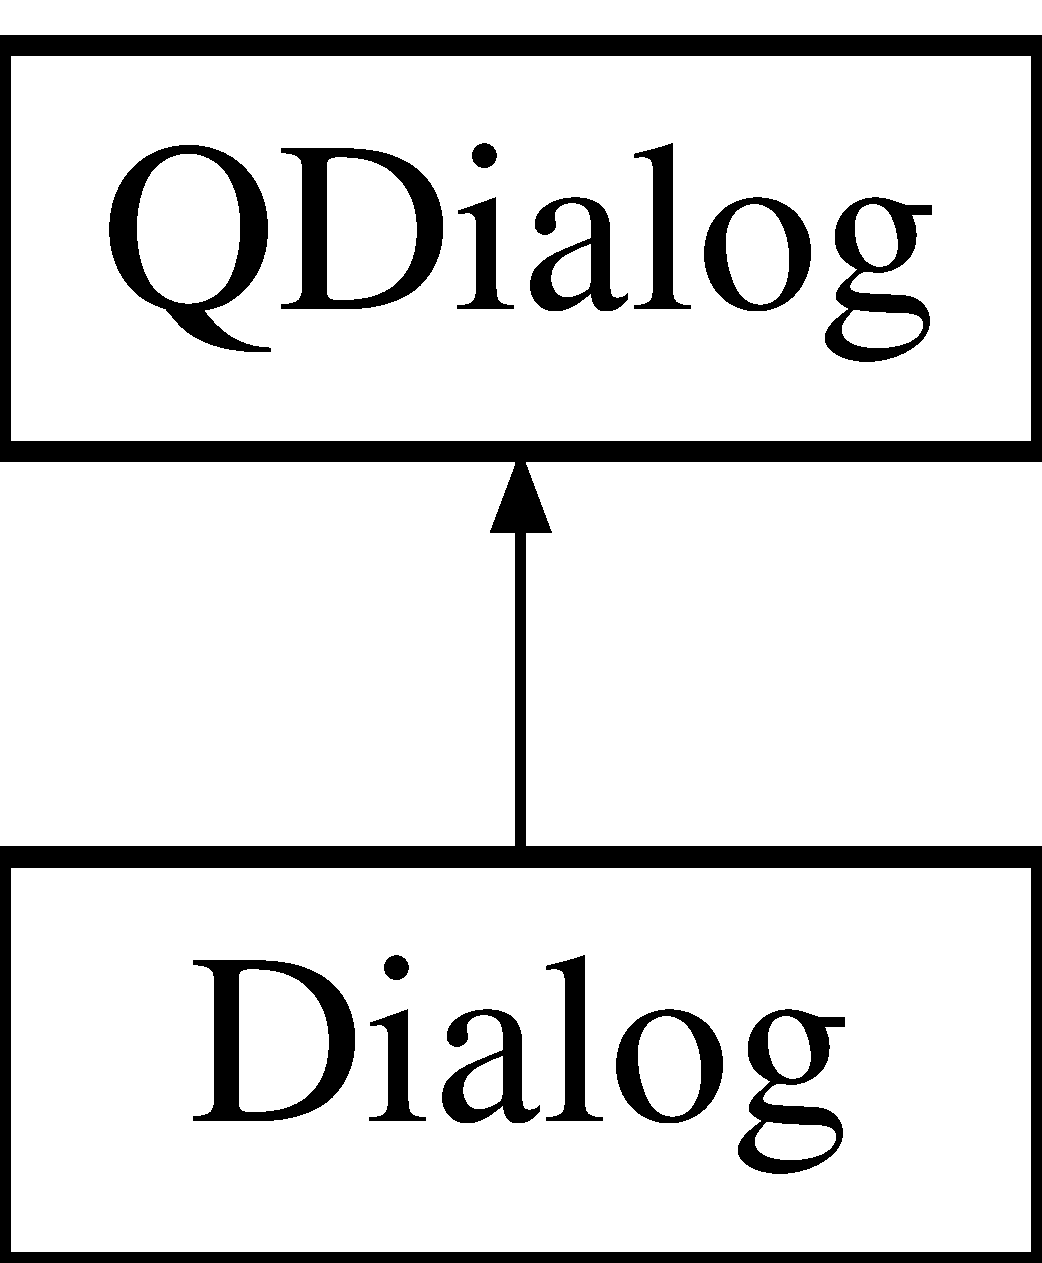
\includegraphics[height=2.000000cm]{class_dialog}
\end{center}
\end{figure}
\subsection*{Signals}
\begin{DoxyCompactItemize}
\item 
void \hyperlink{class_dialog_a5f21e292b0ba87e64682cc7b7a53c7cc}{player\-Changed} ()
\end{DoxyCompactItemize}
\subsection*{Public Member Functions}
\begin{DoxyCompactItemize}
\item 
\hyperlink{class_dialog_a1f16fe034646a987e6de37396e40f674}{Dialog} ()
\begin{DoxyCompactList}\small\item\em \hyperlink{class_dialog_a1f16fe034646a987e6de37396e40f674}{Dialog\-::\-Dialog} Constructor. \end{DoxyCompactList}\item 
\hyperlink{class_dialog_a2a1fe6ef28513eed13bfcd3a4da83ccb}{$\sim$\-Dialog} ()
\begin{DoxyCompactList}\small\item\em \hyperlink{class_dialog_a2a1fe6ef28513eed13bfcd3a4da83ccb}{Dialog\-::$\sim$\-Dialog} Destructor. \end{DoxyCompactList}\item 
void \hyperlink{class_dialog_a4320f72d8354f94942348b74323a651e}{setup\-Game} ()
\begin{DoxyCompactList}\small\item\em \hyperlink{class_dialog_a4320f72d8354f94942348b74323a651e}{Dialog\-::setup\-Game} Sets up the game. \end{DoxyCompactList}\item 
void \hyperlink{class_dialog_a0c2de1df5e1defe8e39bf30afbd63840}{setup\-Dialog} ()
\begin{DoxyCompactList}\small\item\em \hyperlink{class_dialog_a0c2de1df5e1defe8e39bf30afbd63840}{Dialog\-::setup\-Dialog} Sets up the dialog. \end{DoxyCompactList}\end{DoxyCompactItemize}
\subsection*{Private Types}
\begin{DoxyCompactItemize}
\item 
enum \{ \hyperlink{class_dialog_aa450168d087018adecfc85aad9dc0758ad9cc094540b183d393105bd9b90bfd2c}{Num\-Buttons} = 7
 \}
\end{DoxyCompactItemize}
\subsection*{Private Slots}
\begin{DoxyCompactItemize}
\item 
void \hyperlink{class_dialog_a07edaf041e6001503c4ef6291ca557ea}{on\-\_\-new\-Game\-\_\-selected} ()
\begin{DoxyCompactList}\small\item\em \hyperlink{class_dialog_a07edaf041e6001503c4ef6291ca557ea}{Dialog\-::on\-\_\-new\-Game\-\_\-selected} Sets up a new game. \end{DoxyCompactList}\item 
void \hyperlink{class_dialog_a87138e5c0a7a9fefab5549695686117a}{on\-\_\-player\-Changed} ()
\begin{DoxyCompactList}\small\item\em \hyperlink{class_dialog_a87138e5c0a7a9fefab5549695686117a}{Dialog\-::on\-\_\-player\-Changed} Slot for when the player is changed. \end{DoxyCompactList}\end{DoxyCompactItemize}
\subsection*{Private Member Functions}
\begin{DoxyCompactItemize}
\item 
void \hyperlink{class_dialog_a0d839dd1406b5bd21d1e87172d9ba280}{create\-Menu} ()
\begin{DoxyCompactList}\small\item\em \hyperlink{class_dialog_a0d839dd1406b5bd21d1e87172d9ba280}{Dialog\-::create\-Menu} Creates the menu. \end{DoxyCompactList}\item 
void \hyperlink{class_dialog_ab91c0d44d997ee5dc3c9f43866674ec1}{setup\-Players} (int)
\begin{DoxyCompactList}\small\item\em \hyperlink{class_dialog_ab91c0d44d997ee5dc3c9f43866674ec1}{Dialog\-::setup\-Players} Sets up the players. \end{DoxyCompactList}\item 
void \hyperlink{class_dialog_a0815afc1d0d96fd6e1e3f92a8e017aeb}{create\-Horizontal\-Group\-Box} ()
\begin{DoxyCompactList}\small\item\em \hyperlink{class_dialog_a0815afc1d0d96fd6e1e3f92a8e017aeb}{Dialog\-::create\-Horizontal\-Group\-Box} Creates the rack and buttons. \end{DoxyCompactList}\item 
void \hyperlink{class_dialog_a1801636f9eaba94d525a6d174608d4ca}{create\-Grid\-Group\-Box} ()
\begin{DoxyCompactList}\small\item\em \hyperlink{class_dialog_a1801636f9eaba94d525a6d174608d4ca}{Dialog\-::create\-Grid\-Group\-Box} Creates the playing board. \end{DoxyCompactList}\item 
void \hyperlink{class_dialog_a5b7a947ae39abb184aca126baaf5b574}{create\-Form\-Group\-Box} ()
\item 
void \hyperlink{class_dialog_a3e7333b738c6b84b861dac7ea957244a}{create\-Label\-Group\-Box} ()
\begin{DoxyCompactList}\small\item\em \hyperlink{class_dialog_a3e7333b738c6b84b861dac7ea957244a}{Dialog\-::create\-Label\-Group\-Box} Creates the labels that represent the players. \end{DoxyCompactList}\item 
void \hyperlink{class_dialog_a40d6cd5ec81c87ff483fb399075963b3}{load\-Dictionary} ()
\begin{DoxyCompactList}\small\item\em \hyperlink{class_dialog_a40d6cd5ec81c87ff483fb399075963b3}{Dialog\-::load\-Dictionary} Loads the dictionary. \end{DoxyCompactList}\end{DoxyCompactItemize}
\subsection*{Private Attributes}
\begin{DoxyCompactItemize}
\item 
Q\-Menu\-Bar $\ast$ \hyperlink{class_dialog_a9712b5e90ad0a47d97d27bb2648e753b}{menu\-Bar}
\item 
Q\-Group\-Box $\ast$ \hyperlink{class_dialog_a382454f1112e8cf8823979456823e9fc}{horizontal\-Group\-Box}
\item 
Q\-Group\-Box $\ast$ \hyperlink{class_dialog_a93c838af40eaab2aecbc11f4ec2f3680}{grid\-Group\-Box}
\item 
Q\-Group\-Box $\ast$ \hyperlink{class_dialog_a93ffff453dba285f896156d073d58220}{label\-Group\-Box}
\item 
Q\-Push\-Button $\ast$ \hyperlink{class_dialog_aa353f9ab09ea36fb2fdc5e5964b9b2b4}{cancel}
\item 
Q\-Push\-Button $\ast$ \hyperlink{class_dialog_afda3b2243f835037bfeb1322289e4f5a}{play}
\item 
Q\-Push\-Button $\ast$ \hyperlink{class_dialog_a1296240f36b4a11c4cf70a709aced623}{pass}
\item 
Q\-Menu $\ast$ \hyperlink{class_dialog_a266ec552501a452ce6925589823e8484}{file\-Menu}
\item 
Q\-Action $\ast$ \hyperlink{class_dialog_a8b086eb4a5d1ec32a4ddfc3abe705505}{new\-Game\-Action}
\item 
Q\-Action $\ast$ \hyperlink{class_dialog_abf163ec5a4490e0019241f39e3e81b48}{exit\-Action}
\item 
\hyperlink{class_board}{Board} $\ast$ \hyperlink{class_dialog_a0a45509f1cb59a221eb09f16e1ca4923}{board}
\item 
\hyperlink{class_rack}{Rack} $\ast$ \hyperlink{class_dialog_a717eee5215d28c0f10bde1444cb959ed}{rack}
\item 
\hyperlink{class_game}{Game} $\ast$ \hyperlink{class_dialog_a1b67d47768a815f0b2824957bd955c49}{game}
\item 
\hyperlink{class_dictionary}{Dictionary} $\ast$ \hyperlink{class_dialog_a465c936ff76ad97698bde2a9b065ab65}{dictionary}
\item 
vector$<$ \hyperlink{class_player}{Player} $\ast$ $>$ \hyperlink{class_dialog_a93e79b9554adff375010cc56a29c82b0}{players}
\item 
short int \hyperlink{class_dialog_a5130628f920537a9359fbdc4058af7b7}{player\-\_\-cnt}
\end{DoxyCompactItemize}


\subsection{Detailed Description}
The \hyperlink{class_dialog}{Dialog} class Main U\-I class. 

Definition at line 20 of file dialog.\-h.



\subsection{Member Enumeration Documentation}
\hypertarget{class_dialog_aa450168d087018adecfc85aad9dc0758}{\subsubsection[{anonymous enum}]{\setlength{\rightskip}{0pt plus 5cm}anonymous enum\hspace{0.3cm}{\ttfamily [private]}}}\label{class_dialog_aa450168d087018adecfc85aad9dc0758}
\begin{Desc}
\item[Enumerator]\par
\begin{description}
\index{Num\-Buttons@{Num\-Buttons}!Dialog@{Dialog}}\index{Dialog@{Dialog}!Num\-Buttons@{Num\-Buttons}}\item[{\em 
\hypertarget{class_dialog_aa450168d087018adecfc85aad9dc0758ad9cc094540b183d393105bd9b90bfd2c}{Num\-Buttons}\label{class_dialog_aa450168d087018adecfc85aad9dc0758ad9cc094540b183d393105bd9b90bfd2c}
}]\end{description}
\end{Desc}


Definition at line 30 of file dialog.\-h.


\begin{DoxyCode}
30 \{ \hyperlink{class_dialog_aa450168d087018adecfc85aad9dc0758ad9cc094540b183d393105bd9b90bfd2c}{NumButtons} = 7 \};
\end{DoxyCode}


\subsection{Constructor \& Destructor Documentation}
\hypertarget{class_dialog_a1f16fe034646a987e6de37396e40f674}{\index{Dialog@{Dialog}!Dialog@{Dialog}}
\index{Dialog@{Dialog}!Dialog@{Dialog}}
\subsubsection[{Dialog}]{\setlength{\rightskip}{0pt plus 5cm}Dialog\-::\-Dialog (
\begin{DoxyParamCaption}
{}
\end{DoxyParamCaption}
)}}\label{class_dialog_a1f16fe034646a987e6de37396e40f674}


\hyperlink{class_dialog_a1f16fe034646a987e6de37396e40f674}{Dialog\-::\-Dialog} Constructor. 



Definition at line 12 of file dialog.\-cpp.



References board, Board\-::get\-Board(), Rack\-::get\-Rack(), load\-Dictionary(), rack, setup\-Dialog(), setup\-Game(), and setup\-Players().


\begin{DoxyCode}
13 \{
14     \hyperlink{class_dialog_a40d6cd5ec81c87ff483fb399075963b3}{loadDictionary}();
15     \hyperlink{class_dialog_ab91c0d44d997ee5dc3c9f43866674ec1}{setupPlayers}(2);
16 
17     \hyperlink{class_dialog_a0a45509f1cb59a221eb09f16e1ca4923}{board} = \hyperlink{class_board_ae30e802b1d83309fc95e695b5b3df338}{Board::getBoard}();
18     \hyperlink{class_dialog_a717eee5215d28c0f10bde1444cb959ed}{rack} = \hyperlink{class_rack_aa48de650c15bda8267451d84caf6ea3f}{Rack::getRack}();
19     \hyperlink{class_dialog_a4320f72d8354f94942348b74323a651e}{setupGame}();
20     connect(\hyperlink{class_dialog_a0a45509f1cb59a221eb09f16e1ca4923}{board}, SIGNAL(invalidMove()), \hyperlink{class_dialog_a717eee5215d28c0f10bde1444cb959ed}{rack}, SLOT(on\_invalidMove()));
21 
22     \hyperlink{class_dialog_a0c2de1df5e1defe8e39bf30afbd63840}{setupDialog}();
23 \}
\end{DoxyCode}
\hypertarget{class_dialog_a2a1fe6ef28513eed13bfcd3a4da83ccb}{\index{Dialog@{Dialog}!$\sim$\-Dialog@{$\sim$\-Dialog}}
\index{$\sim$\-Dialog@{$\sim$\-Dialog}!Dialog@{Dialog}}
\subsubsection[{$\sim$\-Dialog}]{\setlength{\rightskip}{0pt plus 5cm}Dialog\-::$\sim$\-Dialog (
\begin{DoxyParamCaption}
{}
\end{DoxyParamCaption}
)}}\label{class_dialog_a2a1fe6ef28513eed13bfcd3a4da83ccb}


\hyperlink{class_dialog_a2a1fe6ef28513eed13bfcd3a4da83ccb}{Dialog\-::$\sim$\-Dialog} Destructor. 



Definition at line 28 of file dialog.\-cpp.



References dictionary, game, and players.


\begin{DoxyCode}
28                 \{
29     \textcolor{keywordflow}{while}(!\hyperlink{class_dialog_a93e79b9554adff375010cc56a29c82b0}{players}.empty())\{
30         \textcolor{keyword}{delete} \hyperlink{class_dialog_a93e79b9554adff375010cc56a29c82b0}{players}.back();
31         \hyperlink{class_dialog_a93e79b9554adff375010cc56a29c82b0}{players}.pop\_back();
32     \}
33     \textcolor{keyword}{delete} \hyperlink{class_dialog_a1b67d47768a815f0b2824957bd955c49}{game};
34     \textcolor{keyword}{delete} \hyperlink{class_dialog_a465c936ff76ad97698bde2a9b065ab65}{dictionary};
35 \}
\end{DoxyCode}


\subsection{Member Function Documentation}
\hypertarget{class_dialog_a5b7a947ae39abb184aca126baaf5b574}{\index{Dialog@{Dialog}!create\-Form\-Group\-Box@{create\-Form\-Group\-Box}}
\index{create\-Form\-Group\-Box@{create\-Form\-Group\-Box}!Dialog@{Dialog}}
\subsubsection[{create\-Form\-Group\-Box}]{\setlength{\rightskip}{0pt plus 5cm}void Dialog\-::create\-Form\-Group\-Box (
\begin{DoxyParamCaption}
{}
\end{DoxyParamCaption}
)\hspace{0.3cm}{\ttfamily [private]}}}\label{class_dialog_a5b7a947ae39abb184aca126baaf5b574}
\hypertarget{class_dialog_a1801636f9eaba94d525a6d174608d4ca}{\index{Dialog@{Dialog}!create\-Grid\-Group\-Box@{create\-Grid\-Group\-Box}}
\index{create\-Grid\-Group\-Box@{create\-Grid\-Group\-Box}!Dialog@{Dialog}}
\subsubsection[{create\-Grid\-Group\-Box}]{\setlength{\rightskip}{0pt plus 5cm}void Dialog\-::create\-Grid\-Group\-Box (
\begin{DoxyParamCaption}
{}
\end{DoxyParamCaption}
)\hspace{0.3cm}{\ttfamily [private]}}}\label{class_dialog_a1801636f9eaba94d525a6d174608d4ca}


\hyperlink{class_dialog_a1801636f9eaba94d525a6d174608d4ca}{Dialog\-::create\-Grid\-Group\-Box} Creates the playing board. 



Definition at line 188 of file dialog.\-cpp.



References board, grid\-Group\-Box, and Board\-::spaces.



Referenced by setup\-Dialog().


\begin{DoxyCode}
189 \{
190     \hyperlink{class_dialog_a93c838af40eaab2aecbc11f4ec2f3680}{gridGroupBox} = \textcolor{keyword}{new} QGroupBox();
191     QGridLayout *layout = \textcolor{keyword}{new} QGridLayout;
192     layout->setContentsMargins(0,0,0,0);
193     layout->setSpacing(0);
194     \textcolor{keywordflow}{for} (\textcolor{keywordtype}{int} i = 0; i < 15; i++) \{
195         \textcolor{keywordflow}{for} (\textcolor{keywordtype}{int} j = 0; j < 15; j++) \{
196             layout->addWidget(\hyperlink{class_dialog_a0a45509f1cb59a221eb09f16e1ca4923}{board}->\hyperlink{class_board_a73b12248ddb6ee3adc24f4458d8661c2}{spaces}[i][j], i, j);
197         \}
198     \}
199     \hyperlink{class_dialog_a93c838af40eaab2aecbc11f4ec2f3680}{gridGroupBox}->setLayout(layout);
200 \}
\end{DoxyCode}
\hypertarget{class_dialog_a0815afc1d0d96fd6e1e3f92a8e017aeb}{\index{Dialog@{Dialog}!create\-Horizontal\-Group\-Box@{create\-Horizontal\-Group\-Box}}
\index{create\-Horizontal\-Group\-Box@{create\-Horizontal\-Group\-Box}!Dialog@{Dialog}}
\subsubsection[{create\-Horizontal\-Group\-Box}]{\setlength{\rightskip}{0pt plus 5cm}void Dialog\-::create\-Horizontal\-Group\-Box (
\begin{DoxyParamCaption}
{}
\end{DoxyParamCaption}
)\hspace{0.3cm}{\ttfamily [private]}}}\label{class_dialog_a0815afc1d0d96fd6e1e3f92a8e017aeb}


\hyperlink{class_dialog_a0815afc1d0d96fd6e1e3f92a8e017aeb}{Dialog\-::create\-Horizontal\-Group\-Box} Creates the rack and buttons. 



Definition at line 122 of file dialog.\-cpp.



References cancel, Board\-::get\-Board(), Rack\-::get\-Rack(), Rack\-::get\-Space(), horizontal\-Group\-Box, pass, play, rack, and R\-A\-C\-K\-S\-I\-Z\-E.



Referenced by setup\-Dialog().


\begin{DoxyCode}
123 \{
124     \hyperlink{class_dialog_a382454f1112e8cf8823979456823e9fc}{horizontalGroupBox} = \textcolor{keyword}{new} QGroupBox(tr(\textcolor{stringliteral}{"Player"}));
125     QHBoxLayout *layout = \textcolor{keyword}{new} QHBoxLayout;
126     layout->setContentsMargins(10,10,3,3);
127     layout->setSpacing(0);
128 
129     \textcolor{keywordflow}{for} (\textcolor{keywordtype}{int} i = 0; i < \hyperlink{rack_8h_ad52276b6cc76ff4be1f71000a9094f31}{RACKSIZE}; ++i) \{
130         layout->addWidget(\hyperlink{class_dialog_a717eee5215d28c0f10bde1444cb959ed}{rack}->\hyperlink{class_rack_a2fdfa2264bb85c08ebf107e67cfc8657}{getSpace}(i));
131     \}
132     layout->insertStretch(7);
133     \hyperlink{class_dialog_afda3b2243f835037bfeb1322289e4f5a}{play} = \textcolor{keyword}{new} QPushButton(tr(\textcolor{stringliteral}{"Play"}));
134     layout->addWidget(\hyperlink{class_dialog_afda3b2243f835037bfeb1322289e4f5a}{play});
135     \hyperlink{class_dialog_a1296240f36b4a11c4cf70a709aced623}{pass} = \textcolor{keyword}{new} QPushButton(tr(\textcolor{stringliteral}{"Pass"}));
136     layout->addWidget(\hyperlink{class_dialog_a1296240f36b4a11c4cf70a709aced623}{pass});
137     \hyperlink{class_dialog_aa353f9ab09ea36fb2fdc5e5964b9b2b4}{cancel} = \textcolor{keyword}{new} QPushButton(tr(\textcolor{stringliteral}{"Cancel"}));
138     layout->addWidget(\hyperlink{class_dialog_aa353f9ab09ea36fb2fdc5e5964b9b2b4}{cancel});
139 
140     \hyperlink{class_dialog_a382454f1112e8cf8823979456823e9fc}{horizontalGroupBox}->setLayout(layout);
141 
142     connect(\hyperlink{class_dialog_afda3b2243f835037bfeb1322289e4f5a}{play}, SIGNAL(clicked()), \hyperlink{class_board_ae30e802b1d83309fc95e695b5b3df338}{Board::getBoard}(), SLOT(on\_playButton\_clicked()));
143     connect(\hyperlink{class_dialog_a1296240f36b4a11c4cf70a709aced623}{pass}, SIGNAL(clicked()), \hyperlink{class_board_ae30e802b1d83309fc95e695b5b3df338}{Board::getBoard}(), SLOT(on\_passButton\_clicked()));
144     connect(\hyperlink{class_dialog_aa353f9ab09ea36fb2fdc5e5964b9b2b4}{cancel}, SIGNAL(clicked()), \hyperlink{class_board_ae30e802b1d83309fc95e695b5b3df338}{Board::getBoard}(), SLOT(on\_cancelButton\_clicked
      ()));
145     connect(\hyperlink{class_dialog_aa353f9ab09ea36fb2fdc5e5964b9b2b4}{cancel}, SIGNAL(clicked()), \hyperlink{class_rack_aa48de650c15bda8267451d84caf6ea3f}{Rack::getRack}(), SLOT(on\_cancelButton\_clicked()))
      ;
146 \}
\end{DoxyCode}
\hypertarget{class_dialog_a3e7333b738c6b84b861dac7ea957244a}{\index{Dialog@{Dialog}!create\-Label\-Group\-Box@{create\-Label\-Group\-Box}}
\index{create\-Label\-Group\-Box@{create\-Label\-Group\-Box}!Dialog@{Dialog}}
\subsubsection[{create\-Label\-Group\-Box}]{\setlength{\rightskip}{0pt plus 5cm}void Dialog\-::create\-Label\-Group\-Box (
\begin{DoxyParamCaption}
{}
\end{DoxyParamCaption}
)\hspace{0.3cm}{\ttfamily [private]}}}\label{class_dialog_a3e7333b738c6b84b861dac7ea957244a}


\hyperlink{class_dialog_a3e7333b738c6b84b861dac7ea957244a}{Dialog\-::create\-Label\-Group\-Box} Creates the labels that represent the players. 



Definition at line 152 of file dialog.\-cpp.



References label\-Group\-Box, on\-\_\-player\-Changed(), player\-Changed(), players, Player\-Label\-::set\-Active(), and Player\-Label\-::set\-Inactive().



Referenced by setup\-Dialog().


\begin{DoxyCode}
153 \{
154     \hyperlink{class_dialog_a93ffff453dba285f896156d073d58220}{labelGroupBox} = \textcolor{keyword}{new} QGroupBox();
155     QGridLayout *layout = \textcolor{keyword}{new} QGridLayout;
156     layout->setContentsMargins(0,0,0,0);
157     layout->setSpacing(0);
158     \hyperlink{class_player}{Player}* player;
159 
160     \textcolor{comment}{// create the labels and connect them for each player}
161     \textcolor{keywordflow}{for}(\textcolor{keywordtype}{unsigned} \textcolor{keywordtype}{int} i = 0; i < 4; i++) \{
162         \textcolor{keywordflow}{if} (i < \hyperlink{class_dialog_a93e79b9554adff375010cc56a29c82b0}{players}.size())\{
163              cout << \textcolor{stringliteral}{"setting player"} << endl;
164             player = \hyperlink{class_dialog_a93e79b9554adff375010cc56a29c82b0}{players}[i];
165         \}
166         \textcolor{keywordflow}{else} \{
167             cout << \textcolor{stringliteral}{"setting player to null"} << endl;
168             player = NULL;
169         \}
170         \hyperlink{class_player_label}{PlayerLabel} *label = \textcolor{keyword}{new} \hyperlink{class_player_label}{PlayerLabel}(player);
171         \textcolor{keywordflow}{if} (i == 0)\{
172             label->\hyperlink{class_player_label_a2dfa25456fac3bd2f0a7bbaa4fac6678}{setActive}();
173         \}
174         \textcolor{keywordflow}{else} \{
175             label->\hyperlink{class_player_label_aecd91b6a5f19cd8228869a23bdb7da02}{setInactive}();
176         \}
177         connect(\textcolor{keyword}{this}, SIGNAL(\hyperlink{class_dialog_a5f21e292b0ba87e64682cc7b7a53c7cc}{playerChanged}()), label, SLOT(
      \hyperlink{class_dialog_a87138e5c0a7a9fefab5549695686117a}{on\_playerChanged}()));
178         layout->addWidget(label, i / 2, i % 2);
179     \}
180 
181     \hyperlink{class_dialog_a93ffff453dba285f896156d073d58220}{labelGroupBox}->setLayout(layout);
182 
183 \}
\end{DoxyCode}
\hypertarget{class_dialog_a0d839dd1406b5bd21d1e87172d9ba280}{\index{Dialog@{Dialog}!create\-Menu@{create\-Menu}}
\index{create\-Menu@{create\-Menu}!Dialog@{Dialog}}
\subsubsection[{create\-Menu}]{\setlength{\rightskip}{0pt plus 5cm}void Dialog\-::create\-Menu (
\begin{DoxyParamCaption}
{}
\end{DoxyParamCaption}
)\hspace{0.3cm}{\ttfamily [private]}}}\label{class_dialog_a0d839dd1406b5bd21d1e87172d9ba280}


\hyperlink{class_dialog_a0d839dd1406b5bd21d1e87172d9ba280}{Dialog\-::create\-Menu} Creates the menu. 



Definition at line 105 of file dialog.\-cpp.



References exit\-Action, file\-Menu, menu\-Bar, new\-Game\-Action, and on\-\_\-new\-Game\-\_\-selected().



Referenced by setup\-Dialog().


\begin{DoxyCode}
106 \{
107     \hyperlink{class_dialog_a9712b5e90ad0a47d97d27bb2648e753b}{menuBar} = \textcolor{keyword}{new} QMenuBar;
108 
109     \hyperlink{class_dialog_a266ec552501a452ce6925589823e8484}{fileMenu} = \textcolor{keyword}{new} QMenu(tr(\textcolor{stringliteral}{"&File"}), \textcolor{keyword}{this});
110     \hyperlink{class_dialog_a8b086eb4a5d1ec32a4ddfc3abe705505}{newGameAction} = \hyperlink{class_dialog_a266ec552501a452ce6925589823e8484}{fileMenu}->addAction(tr(\textcolor{stringliteral}{"&New Game"}));
111     \hyperlink{class_dialog_abf163ec5a4490e0019241f39e3e81b48}{exitAction} = \hyperlink{class_dialog_a266ec552501a452ce6925589823e8484}{fileMenu}->addAction(tr(\textcolor{stringliteral}{"E&xit"}));
112     \hyperlink{class_dialog_a9712b5e90ad0a47d97d27bb2648e753b}{menuBar}->addMenu(\hyperlink{class_dialog_a266ec552501a452ce6925589823e8484}{fileMenu});
113 
114     connect(\hyperlink{class_dialog_a8b086eb4a5d1ec32a4ddfc3abe705505}{newGameAction}, SIGNAL(triggered()), \textcolor{keyword}{this}, SLOT(
      \hyperlink{class_dialog_a07edaf041e6001503c4ef6291ca557ea}{on\_newGame\_selected}()));
115     connect(\hyperlink{class_dialog_abf163ec5a4490e0019241f39e3e81b48}{exitAction}, SIGNAL(triggered()), \textcolor{keyword}{this}, SLOT(accept()));
116 \}
\end{DoxyCode}
\hypertarget{class_dialog_a40d6cd5ec81c87ff483fb399075963b3}{\index{Dialog@{Dialog}!load\-Dictionary@{load\-Dictionary}}
\index{load\-Dictionary@{load\-Dictionary}!Dialog@{Dialog}}
\subsubsection[{load\-Dictionary}]{\setlength{\rightskip}{0pt plus 5cm}void Dialog\-::load\-Dictionary (
\begin{DoxyParamCaption}
{}
\end{DoxyParamCaption}
)\hspace{0.3cm}{\ttfamily [private]}}}\label{class_dialog_a40d6cd5ec81c87ff483fb399075963b3}


\hyperlink{class_dialog_a40d6cd5ec81c87ff483fb399075963b3}{Dialog\-::load\-Dictionary} Loads the dictionary. 



Definition at line 95 of file dialog.\-cpp.



References dictionary, and Dictionary\-Loader\-::load().



Referenced by Dialog().


\begin{DoxyCode}
95                            \{
96     \hyperlink{class_dialog_a465c936ff76ad97698bde2a9b065ab65}{dictionary} = \textcolor{keyword}{new} \hyperlink{class_dictionary}{Dictionary}();
97     \hyperlink{class_dictionary_loader}{DictionaryLoader} *dictionaryLoader = \textcolor{keyword}{new} \hyperlink{class_dictionary_loader}{DictionaryLoader}(
      \hyperlink{class_dialog_a465c936ff76ad97698bde2a9b065ab65}{dictionary}, \textcolor{stringliteral}{":/resources/dictionary.txt"});
98     dictionaryLoader->\hyperlink{class_dictionary_loader_a1441785d7f5a848be0d7b7f432e338f8}{load}();
99     \textcolor{keyword}{delete} dictionaryLoader;
100 \}
\end{DoxyCode}
\hypertarget{class_dialog_a07edaf041e6001503c4ef6291ca557ea}{\index{Dialog@{Dialog}!on\-\_\-new\-Game\-\_\-selected@{on\-\_\-new\-Game\-\_\-selected}}
\index{on\-\_\-new\-Game\-\_\-selected@{on\-\_\-new\-Game\-\_\-selected}!Dialog@{Dialog}}
\subsubsection[{on\-\_\-new\-Game\-\_\-selected}]{\setlength{\rightskip}{0pt plus 5cm}void Dialog\-::on\-\_\-new\-Game\-\_\-selected (
\begin{DoxyParamCaption}
{}
\end{DoxyParamCaption}
)\hspace{0.3cm}{\ttfamily [private]}, {\ttfamily [slot]}}}\label{class_dialog_a07edaf041e6001503c4ef6291ca557ea}


\hyperlink{class_dialog_a07edaf041e6001503c4ef6291ca557ea}{Dialog\-::on\-\_\-new\-Game\-\_\-selected} Sets up a new game. 



Definition at line 205 of file dialog.\-cpp.



References board, game, players, Board\-::reset(), and setup\-Game().



Referenced by create\-Menu().


\begin{DoxyCode}
206 \{
207     \textcolor{keywordflow}{if} (\hyperlink{class_dialog_a1b67d47768a815f0b2824957bd955c49}{game} != NULL)\{
208         \textcolor{keyword}{delete}(\hyperlink{class_dialog_a1b67d47768a815f0b2824957bd955c49}{game});
209         \hyperlink{class_dialog_a1b67d47768a815f0b2824957bd955c49}{game} = NULL;
210     \}
211     \textcolor{keywordflow}{for} (\textcolor{keywordtype}{unsigned} \textcolor{keywordtype}{int} i = 0; i < \hyperlink{class_dialog_a93e79b9554adff375010cc56a29c82b0}{players}.size(); i++)\{
212         \hyperlink{class_dialog_a93e79b9554adff375010cc56a29c82b0}{players}.at(i)->clearScore();
213     \}
214     \hyperlink{class_dialog_a0a45509f1cb59a221eb09f16e1ca4923}{board}->\hyperlink{class_board_a13c88b0bc7d2a85f7e53790e71bdd403}{reset}();
215     \hyperlink{class_dialog_a4320f72d8354f94942348b74323a651e}{setupGame}();
216 
217 \}
\end{DoxyCode}
\hypertarget{class_dialog_a87138e5c0a7a9fefab5549695686117a}{\index{Dialog@{Dialog}!on\-\_\-player\-Changed@{on\-\_\-player\-Changed}}
\index{on\-\_\-player\-Changed@{on\-\_\-player\-Changed}!Dialog@{Dialog}}
\subsubsection[{on\-\_\-player\-Changed}]{\setlength{\rightskip}{0pt plus 5cm}void Dialog\-::on\-\_\-player\-Changed (
\begin{DoxyParamCaption}
{}
\end{DoxyParamCaption}
)\hspace{0.3cm}{\ttfamily [private]}, {\ttfamily [slot]}}}\label{class_dialog_a87138e5c0a7a9fefab5549695686117a}


\hyperlink{class_dialog_a87138e5c0a7a9fefab5549695686117a}{Dialog\-::on\-\_\-player\-Changed} Slot for when the player is changed. 



Definition at line 222 of file dialog.\-cpp.



References player\-Changed().



Referenced by create\-Label\-Group\-Box(), and setup\-Game().


\begin{DoxyCode}
223 \{
224     cout << \textcolor{stringliteral}{"Dialog is emitting an on\_playerChanged() signal."} << endl;
225     emit (\hyperlink{class_dialog_a5f21e292b0ba87e64682cc7b7a53c7cc}{playerChanged}());
226 \}
\end{DoxyCode}
\hypertarget{class_dialog_a5f21e292b0ba87e64682cc7b7a53c7cc}{\index{Dialog@{Dialog}!player\-Changed@{player\-Changed}}
\index{player\-Changed@{player\-Changed}!Dialog@{Dialog}}
\subsubsection[{player\-Changed}]{\setlength{\rightskip}{0pt plus 5cm}void Dialog\-::player\-Changed (
\begin{DoxyParamCaption}
{}
\end{DoxyParamCaption}
)\hspace{0.3cm}{\ttfamily [signal]}}}\label{class_dialog_a5f21e292b0ba87e64682cc7b7a53c7cc}


Referenced by create\-Label\-Group\-Box(), on\-\_\-player\-Changed(), and setup\-Game().

\hypertarget{class_dialog_a0c2de1df5e1defe8e39bf30afbd63840}{\index{Dialog@{Dialog}!setup\-Dialog@{setup\-Dialog}}
\index{setup\-Dialog@{setup\-Dialog}!Dialog@{Dialog}}
\subsubsection[{setup\-Dialog}]{\setlength{\rightskip}{0pt plus 5cm}void Dialog\-::setup\-Dialog (
\begin{DoxyParamCaption}
{}
\end{DoxyParamCaption}
)}}\label{class_dialog_a0c2de1df5e1defe8e39bf30afbd63840}


\hyperlink{class_dialog_a0c2de1df5e1defe8e39bf30afbd63840}{Dialog\-::setup\-Dialog} Sets up the dialog. 

\begin{DoxyRefDesc}{Todo}
\item[\hyperlink{todo__todo000002}{Todo}]this is not great, but the only way I could disable resizing on Linux \end{DoxyRefDesc}


Definition at line 52 of file dialog.\-cpp.



References create\-Grid\-Group\-Box(), create\-Horizontal\-Group\-Box(), create\-Label\-Group\-Box(), create\-Menu(), grid\-Group\-Box, horizontal\-Group\-Box, label\-Group\-Box, and menu\-Bar.



Referenced by Dialog().


\begin{DoxyCode}
53 \{
54     \hyperlink{class_dialog_a0d839dd1406b5bd21d1e87172d9ba280}{createMenu}();
55     \hyperlink{class_dialog_a0815afc1d0d96fd6e1e3f92a8e017aeb}{createHorizontalGroupBox}();
56     \hyperlink{class_dialog_a1801636f9eaba94d525a6d174608d4ca}{createGridGroupBox}();
57     \hyperlink{class_dialog_a3e7333b738c6b84b861dac7ea957244a}{createLabelGroupBox}();
58 
59     QVBoxLayout *mainLayout = \textcolor{keyword}{new} QVBoxLayout;
60     mainLayout->setMenuBar(\hyperlink{class_dialog_a9712b5e90ad0a47d97d27bb2648e753b}{menuBar});
61     mainLayout->addWidget(\hyperlink{class_dialog_a93c838af40eaab2aecbc11f4ec2f3680}{gridGroupBox});
62     mainLayout->addWidget(\hyperlink{class_dialog_a382454f1112e8cf8823979456823e9fc}{horizontalGroupBox});
63     mainLayout->addWidget(\hyperlink{class_dialog_a93ffff453dba285f896156d073d58220}{labelGroupBox});
64 
65     setLayout(mainLayout);
66     setWindowTitle(tr(\textcolor{stringliteral}{"Words for CS 340 Students"}));
67 
70     setFixedSize(580, 700);
71 \}
\end{DoxyCode}
\hypertarget{class_dialog_a4320f72d8354f94942348b74323a651e}{\index{Dialog@{Dialog}!setup\-Game@{setup\-Game}}
\index{setup\-Game@{setup\-Game}!Dialog@{Dialog}}
\subsubsection[{setup\-Game}]{\setlength{\rightskip}{0pt plus 5cm}void Dialog\-::setup\-Game (
\begin{DoxyParamCaption}
{}
\end{DoxyParamCaption}
)}}\label{class_dialog_a4320f72d8354f94942348b74323a651e}


\hyperlink{class_dialog_a4320f72d8354f94942348b74323a651e}{Dialog\-::setup\-Game} Sets up the game. 



Definition at line 40 of file dialog.\-cpp.



References board, dictionary, game, on\-\_\-player\-Changed(), player\-Changed(), players, rack, Rack\-::refresh(), and Board\-::set\-Game().



Referenced by Dialog(), and on\-\_\-new\-Game\-\_\-selected().


\begin{DoxyCode}
41 \{
42     \hyperlink{class_dialog_a1b67d47768a815f0b2824957bd955c49}{game} = \textcolor{keyword}{new} \hyperlink{class_game}{Game}(\hyperlink{class_dialog_a93e79b9554adff375010cc56a29c82b0}{players}, \hyperlink{class_dialog_a465c936ff76ad97698bde2a9b065ab65}{dictionary});
43     \hyperlink{class_dialog_a0a45509f1cb59a221eb09f16e1ca4923}{board}->\hyperlink{class_board_ae08098fe478e2832e7e7403140314164}{setGame}(\hyperlink{class_dialog_a1b67d47768a815f0b2824957bd955c49}{game});
44     \hyperlink{class_dialog_a717eee5215d28c0f10bde1444cb959ed}{rack}->\hyperlink{class_rack_ae1b5a6e15cb1ebe299356959b6a8d641}{refresh}(\hyperlink{class_dialog_a1b67d47768a815f0b2824957bd955c49}{game});
45     connect(\hyperlink{class_dialog_a1b67d47768a815f0b2824957bd955c49}{game}, SIGNAL(\hyperlink{class_dialog_a5f21e292b0ba87e64682cc7b7a53c7cc}{playerChanged}()), \textcolor{keyword}{this}, SLOT(
      \hyperlink{class_dialog_a87138e5c0a7a9fefab5549695686117a}{on\_playerChanged}()));
46     emit(\hyperlink{class_dialog_a5f21e292b0ba87e64682cc7b7a53c7cc}{playerChanged}());
47 \}
\end{DoxyCode}
\hypertarget{class_dialog_ab91c0d44d997ee5dc3c9f43866674ec1}{\index{Dialog@{Dialog}!setup\-Players@{setup\-Players}}
\index{setup\-Players@{setup\-Players}!Dialog@{Dialog}}
\subsubsection[{setup\-Players}]{\setlength{\rightskip}{0pt plus 5cm}void Dialog\-::setup\-Players (
\begin{DoxyParamCaption}
\item[{int}]{num}
\end{DoxyParamCaption}
)\hspace{0.3cm}{\ttfamily [private]}}}\label{class_dialog_ab91c0d44d997ee5dc3c9f43866674ec1}


\hyperlink{class_dialog_ab91c0d44d997ee5dc3c9f43866674ec1}{Dialog\-::setup\-Players} Sets up the players. 


\begin{DoxyParams}{Parameters}
{\em num} & The number of players to set up \\
\hline
\end{DoxyParams}


Definition at line 77 of file dialog.\-cpp.



References A\-I\-Player\-::\-A\-I\-Player(), and players.



Referenced by Dialog().


\begin{DoxyCode}
78 \{
79     \textcolor{keywordflow}{for} (\textcolor{keywordtype}{int} i = 0; i < num; i++)\{
80         QString *playerName = \textcolor{keyword}{new} QString(\textcolor{stringliteral}{"Player "} + QString::number(i + 1));
81         \textcolor{keywordflow}{if} (i == 0)\{
82             \hyperlink{class_dialog_a93e79b9554adff375010cc56a29c82b0}{players}.push\_back(\textcolor{keyword}{new} \hyperlink{class_human_player}{HumanPlayer}(*playerName));
83         \}
84         \textcolor{keywordflow}{else} \{
85             \textcolor{comment}{// players.push\_back(new HumanPlayer(*playerName));}
86             \hyperlink{class_dialog_a93e79b9554adff375010cc56a29c82b0}{players}.push\_back(\textcolor{keyword}{new} \hyperlink{class_a_i_player}{AIPlayer}(*playerName));
87         \}
88         cout << \hyperlink{class_dialog_a93e79b9554adff375010cc56a29c82b0}{players}.back()->getName().toStdString();
89     \};
90 \}
\end{DoxyCode}


\subsection{Member Data Documentation}
\hypertarget{class_dialog_a0a45509f1cb59a221eb09f16e1ca4923}{\index{Dialog@{Dialog}!board@{board}}
\index{board@{board}!Dialog@{Dialog}}
\subsubsection[{board}]{\setlength{\rightskip}{0pt plus 5cm}{\bf Board}$\ast$ Dialog\-::board\hspace{0.3cm}{\ttfamily [private]}}}\label{class_dialog_a0a45509f1cb59a221eb09f16e1ca4923}
The \hyperlink{class_board}{Board} 

Definition at line 45 of file dialog.\-h.



Referenced by create\-Grid\-Group\-Box(), Dialog(), on\-\_\-new\-Game\-\_\-selected(), and setup\-Game().

\hypertarget{class_dialog_aa353f9ab09ea36fb2fdc5e5964b9b2b4}{\index{Dialog@{Dialog}!cancel@{cancel}}
\index{cancel@{cancel}!Dialog@{Dialog}}
\subsubsection[{cancel}]{\setlength{\rightskip}{0pt plus 5cm}Q\-Push\-Button$\ast$ Dialog\-::cancel\hspace{0.3cm}{\ttfamily [private]}}}\label{class_dialog_aa353f9ab09ea36fb2fdc5e5964b9b2b4}
The cancel button 

Definition at line 37 of file dialog.\-h.



Referenced by create\-Horizontal\-Group\-Box().

\hypertarget{class_dialog_a465c936ff76ad97698bde2a9b065ab65}{\index{Dialog@{Dialog}!dictionary@{dictionary}}
\index{dictionary@{dictionary}!Dialog@{Dialog}}
\subsubsection[{dictionary}]{\setlength{\rightskip}{0pt plus 5cm}{\bf Dictionary}$\ast$ Dialog\-::dictionary\hspace{0.3cm}{\ttfamily [private]}}}\label{class_dialog_a465c936ff76ad97698bde2a9b065ab65}
The \hyperlink{class_dictionary}{Dictionary} 

Definition at line 48 of file dialog.\-h.



Referenced by load\-Dictionary(), setup\-Game(), and $\sim$\-Dialog().

\hypertarget{class_dialog_abf163ec5a4490e0019241f39e3e81b48}{\index{Dialog@{Dialog}!exit\-Action@{exit\-Action}}
\index{exit\-Action@{exit\-Action}!Dialog@{Dialog}}
\subsubsection[{exit\-Action}]{\setlength{\rightskip}{0pt plus 5cm}Q\-Action$\ast$ Dialog\-::exit\-Action\hspace{0.3cm}{\ttfamily [private]}}}\label{class_dialog_abf163ec5a4490e0019241f39e3e81b48}
Action when the user chooses to exit 

Definition at line 43 of file dialog.\-h.



Referenced by create\-Menu().

\hypertarget{class_dialog_a266ec552501a452ce6925589823e8484}{\index{Dialog@{Dialog}!file\-Menu@{file\-Menu}}
\index{file\-Menu@{file\-Menu}!Dialog@{Dialog}}
\subsubsection[{file\-Menu}]{\setlength{\rightskip}{0pt plus 5cm}Q\-Menu$\ast$ Dialog\-::file\-Menu\hspace{0.3cm}{\ttfamily [private]}}}\label{class_dialog_a266ec552501a452ce6925589823e8484}
The file menu 

Definition at line 41 of file dialog.\-h.



Referenced by create\-Menu().

\hypertarget{class_dialog_a1b67d47768a815f0b2824957bd955c49}{\index{Dialog@{Dialog}!game@{game}}
\index{game@{game}!Dialog@{Dialog}}
\subsubsection[{game}]{\setlength{\rightskip}{0pt plus 5cm}{\bf Game}$\ast$ Dialog\-::game\hspace{0.3cm}{\ttfamily [private]}}}\label{class_dialog_a1b67d47768a815f0b2824957bd955c49}
The \hyperlink{class_game}{Game} 

Definition at line 47 of file dialog.\-h.



Referenced by on\-\_\-new\-Game\-\_\-selected(), setup\-Game(), and $\sim$\-Dialog().

\hypertarget{class_dialog_a93c838af40eaab2aecbc11f4ec2f3680}{\index{Dialog@{Dialog}!grid\-Group\-Box@{grid\-Group\-Box}}
\index{grid\-Group\-Box@{grid\-Group\-Box}!Dialog@{Dialog}}
\subsubsection[{grid\-Group\-Box}]{\setlength{\rightskip}{0pt plus 5cm}Q\-Group\-Box$\ast$ Dialog\-::grid\-Group\-Box\hspace{0.3cm}{\ttfamily [private]}}}\label{class_dialog_a93c838af40eaab2aecbc11f4ec2f3680}
A grid group box 

Definition at line 34 of file dialog.\-h.



Referenced by create\-Grid\-Group\-Box(), and setup\-Dialog().

\hypertarget{class_dialog_a382454f1112e8cf8823979456823e9fc}{\index{Dialog@{Dialog}!horizontal\-Group\-Box@{horizontal\-Group\-Box}}
\index{horizontal\-Group\-Box@{horizontal\-Group\-Box}!Dialog@{Dialog}}
\subsubsection[{horizontal\-Group\-Box}]{\setlength{\rightskip}{0pt plus 5cm}Q\-Group\-Box$\ast$ Dialog\-::horizontal\-Group\-Box\hspace{0.3cm}{\ttfamily [private]}}}\label{class_dialog_a382454f1112e8cf8823979456823e9fc}
A horizontal group box 

Definition at line 33 of file dialog.\-h.



Referenced by create\-Horizontal\-Group\-Box(), and setup\-Dialog().

\hypertarget{class_dialog_a93ffff453dba285f896156d073d58220}{\index{Dialog@{Dialog}!label\-Group\-Box@{label\-Group\-Box}}
\index{label\-Group\-Box@{label\-Group\-Box}!Dialog@{Dialog}}
\subsubsection[{label\-Group\-Box}]{\setlength{\rightskip}{0pt plus 5cm}Q\-Group\-Box$\ast$ Dialog\-::label\-Group\-Box\hspace{0.3cm}{\ttfamily [private]}}}\label{class_dialog_a93ffff453dba285f896156d073d58220}
A label group box 

Definition at line 35 of file dialog.\-h.



Referenced by create\-Label\-Group\-Box(), and setup\-Dialog().

\hypertarget{class_dialog_a9712b5e90ad0a47d97d27bb2648e753b}{\index{Dialog@{Dialog}!menu\-Bar@{menu\-Bar}}
\index{menu\-Bar@{menu\-Bar}!Dialog@{Dialog}}
\subsubsection[{menu\-Bar}]{\setlength{\rightskip}{0pt plus 5cm}Q\-Menu\-Bar$\ast$ Dialog\-::menu\-Bar\hspace{0.3cm}{\ttfamily [private]}}}\label{class_dialog_a9712b5e90ad0a47d97d27bb2648e753b}
The menu bar 

Definition at line 32 of file dialog.\-h.



Referenced by create\-Menu(), and setup\-Dialog().

\hypertarget{class_dialog_a8b086eb4a5d1ec32a4ddfc3abe705505}{\index{Dialog@{Dialog}!new\-Game\-Action@{new\-Game\-Action}}
\index{new\-Game\-Action@{new\-Game\-Action}!Dialog@{Dialog}}
\subsubsection[{new\-Game\-Action}]{\setlength{\rightskip}{0pt plus 5cm}Q\-Action$\ast$ Dialog\-::new\-Game\-Action\hspace{0.3cm}{\ttfamily [private]}}}\label{class_dialog_a8b086eb4a5d1ec32a4ddfc3abe705505}
Action when the user chooses a new game 

Definition at line 42 of file dialog.\-h.



Referenced by create\-Menu().

\hypertarget{class_dialog_a1296240f36b4a11c4cf70a709aced623}{\index{Dialog@{Dialog}!pass@{pass}}
\index{pass@{pass}!Dialog@{Dialog}}
\subsubsection[{pass}]{\setlength{\rightskip}{0pt plus 5cm}Q\-Push\-Button$\ast$ Dialog\-::pass\hspace{0.3cm}{\ttfamily [private]}}}\label{class_dialog_a1296240f36b4a11c4cf70a709aced623}
The pass button 

Definition at line 39 of file dialog.\-h.



Referenced by create\-Horizontal\-Group\-Box().

\hypertarget{class_dialog_afda3b2243f835037bfeb1322289e4f5a}{\index{Dialog@{Dialog}!play@{play}}
\index{play@{play}!Dialog@{Dialog}}
\subsubsection[{play}]{\setlength{\rightskip}{0pt plus 5cm}Q\-Push\-Button$\ast$ Dialog\-::play\hspace{0.3cm}{\ttfamily [private]}}}\label{class_dialog_afda3b2243f835037bfeb1322289e4f5a}
The play button 

Definition at line 38 of file dialog.\-h.



Referenced by create\-Horizontal\-Group\-Box().

\hypertarget{class_dialog_a5130628f920537a9359fbdc4058af7b7}{\index{Dialog@{Dialog}!player\-\_\-cnt@{player\-\_\-cnt}}
\index{player\-\_\-cnt@{player\-\_\-cnt}!Dialog@{Dialog}}
\subsubsection[{player\-\_\-cnt}]{\setlength{\rightskip}{0pt plus 5cm}short int Dialog\-::player\-\_\-cnt\hspace{0.3cm}{\ttfamily [private]}}}\label{class_dialog_a5130628f920537a9359fbdc4058af7b7}
The number of Players 

Definition at line 50 of file dialog.\-h.

\hypertarget{class_dialog_a93e79b9554adff375010cc56a29c82b0}{\index{Dialog@{Dialog}!players@{players}}
\index{players@{players}!Dialog@{Dialog}}
\subsubsection[{players}]{\setlength{\rightskip}{0pt plus 5cm}vector$<${\bf Player}$\ast$$>$ Dialog\-::players\hspace{0.3cm}{\ttfamily [private]}}}\label{class_dialog_a93e79b9554adff375010cc56a29c82b0}
The Players 

Definition at line 49 of file dialog.\-h.



Referenced by create\-Label\-Group\-Box(), on\-\_\-new\-Game\-\_\-selected(), setup\-Game(), setup\-Players(), and $\sim$\-Dialog().

\hypertarget{class_dialog_a717eee5215d28c0f10bde1444cb959ed}{\index{Dialog@{Dialog}!rack@{rack}}
\index{rack@{rack}!Dialog@{Dialog}}
\subsubsection[{rack}]{\setlength{\rightskip}{0pt plus 5cm}{\bf Rack}$\ast$ Dialog\-::rack\hspace{0.3cm}{\ttfamily [private]}}}\label{class_dialog_a717eee5215d28c0f10bde1444cb959ed}
The \hyperlink{class_rack}{Rack} 

Definition at line 46 of file dialog.\-h.



Referenced by create\-Horizontal\-Group\-Box(), Dialog(), and setup\-Game().



The documentation for this class was generated from the following files\-:\begin{DoxyCompactItemize}
\item 
Scrabble/\hyperlink{dialog_8h}{dialog.\-h}\item 
Scrabble/\hyperlink{dialog_8cpp}{dialog.\-cpp}\end{DoxyCompactItemize}

\hypertarget{class_dictionary}{\section{Dictionary Class Reference}
\label{class_dictionary}\index{Dictionary@{Dictionary}}
}


The \hyperlink{class_dictionary}{Dictionary} class Encapsulates dicitonary operations.  




{\ttfamily \#include $<$dictionary.\-h$>$}

\subsection*{Public Member Functions}
\begin{DoxyCompactItemize}
\item 
\hyperlink{class_dictionary_aee8d612bc9d323c38faba045ba384b8b}{Dictionary} ()
\begin{DoxyCompactList}\small\item\em \hyperlink{class_dictionary_aee8d612bc9d323c38faba045ba384b8b}{Dictionary\-::\-Dictionary} Constructor for dictionary. \end{DoxyCompactList}\item 
\hyperlink{class_dictionary_aa36f24073d9c9001768517aa2322cb82}{$\sim$\-Dictionary} ()
\begin{DoxyCompactList}\small\item\em \hyperlink{class_dictionary_aa36f24073d9c9001768517aa2322cb82}{Dictionary\-::$\sim$\-Dictionary} Destructor. \end{DoxyCompactList}\item 
bool \hyperlink{class_dictionary_afe2588ce04f6ad733c51df58a8d0d96b}{is\-Word} (Q\-String)
\begin{DoxyCompactList}\small\item\em \hyperlink{class_dictionary_afe2588ce04f6ad733c51df58a8d0d96b}{Dictionary\-::is\-Word} Returns boolean true if is a word. \end{DoxyCompactList}\item 
bool \hyperlink{class_dictionary_a6bf35992b5b44b610b830c2361c67c3e}{add\-Word} (Q\-String, bool)
\begin{DoxyCompactList}\small\item\em \hyperlink{class_dictionary_a6bf35992b5b44b610b830c2361c67c3e}{Dictionary\-::add\-Word} Adds a word to the dictionary. \end{DoxyCompactList}\item 
unsigned \hyperlink{class_dictionary_a327b99a18977f2b898adfd496426cf27}{wordcount} ()
\begin{DoxyCompactList}\small\item\em \hyperlink{class_dictionary_a327b99a18977f2b898adfd496426cf27}{Dictionary\-::wordcount} Getter for word count. \end{DoxyCompactList}\end{DoxyCompactItemize}
\subsection*{Private Attributes}
\begin{DoxyCompactItemize}
\item 
\hyperlink{class_trie}{Trie} $\ast$ \hyperlink{class_dictionary_ac6c08127a37d8131fb8fb1e738406e85}{words}
\item 
unsigned \hyperlink{class_dictionary_aef2de3d2a839832ecc35eb6e08cc9395}{\-\_\-wcount}
\end{DoxyCompactItemize}
\subsection*{Friends}
\begin{DoxyCompactItemize}
\item 
class \hyperlink{class_dictionary_a832b4d233efee1a32feb0f4190b30d39}{Unit\-Test}
\item 
class \hyperlink{class_dictionary_a2c11a076a909acd936d897cd2a81f931}{A\-I\-Player}
\end{DoxyCompactItemize}


\subsection{Detailed Description}
The \hyperlink{class_dictionary}{Dictionary} class Encapsulates dicitonary operations. 

Definition at line 12 of file dictionary.\-h.



\subsection{Constructor \& Destructor Documentation}
\hypertarget{class_dictionary_aee8d612bc9d323c38faba045ba384b8b}{\index{Dictionary@{Dictionary}!Dictionary@{Dictionary}}
\index{Dictionary@{Dictionary}!Dictionary@{Dictionary}}
\subsubsection[{Dictionary}]{\setlength{\rightskip}{0pt plus 5cm}Dictionary\-::\-Dictionary (
\begin{DoxyParamCaption}
{}
\end{DoxyParamCaption}
)}}\label{class_dictionary_aee8d612bc9d323c38faba045ba384b8b}


\hyperlink{class_dictionary_aee8d612bc9d323c38faba045ba384b8b}{Dictionary\-::\-Dictionary} Constructor for dictionary. 



Definition at line 8 of file dictionary.\-cpp.


\begin{DoxyCode}
9 \{
10     \hyperlink{class_dictionary_ac6c08127a37d8131fb8fb1e738406e85}{words} = \textcolor{keyword}{new} \hyperlink{class_trie}{Trie}();
11     \hyperlink{class_dictionary_aef2de3d2a839832ecc35eb6e08cc9395}{\_wcount} = 0;
12 \}
\end{DoxyCode}
\hypertarget{class_dictionary_aa36f24073d9c9001768517aa2322cb82}{\index{Dictionary@{Dictionary}!$\sim$\-Dictionary@{$\sim$\-Dictionary}}
\index{$\sim$\-Dictionary@{$\sim$\-Dictionary}!Dictionary@{Dictionary}}
\subsubsection[{$\sim$\-Dictionary}]{\setlength{\rightskip}{0pt plus 5cm}Dictionary\-::$\sim$\-Dictionary (
\begin{DoxyParamCaption}
{}
\end{DoxyParamCaption}
)}}\label{class_dictionary_aa36f24073d9c9001768517aa2322cb82}


\hyperlink{class_dictionary_aa36f24073d9c9001768517aa2322cb82}{Dictionary\-::$\sim$\-Dictionary} Destructor. 



Definition at line 17 of file dictionary.\-cpp.


\begin{DoxyCode}
18 \{
19     \textcolor{keyword}{delete} \hyperlink{class_dictionary_ac6c08127a37d8131fb8fb1e738406e85}{words};
20 \}
\end{DoxyCode}


\subsection{Member Function Documentation}
\hypertarget{class_dictionary_a6bf35992b5b44b610b830c2361c67c3e}{\index{Dictionary@{Dictionary}!add\-Word@{add\-Word}}
\index{add\-Word@{add\-Word}!Dictionary@{Dictionary}}
\subsubsection[{add\-Word}]{\setlength{\rightskip}{0pt plus 5cm}bool Dictionary\-::add\-Word (
\begin{DoxyParamCaption}
\item[{Q\-String}]{word, }
\item[{bool}]{check\-Word}
\end{DoxyParamCaption}
)}}\label{class_dictionary_a6bf35992b5b44b610b830c2361c67c3e}


\hyperlink{class_dictionary_a6bf35992b5b44b610b830c2361c67c3e}{Dictionary\-::add\-Word} Adds a word to the dictionary. 


\begin{DoxyParams}{Parameters}
{\em word} & The word to add \\
\hline
{\em check\-Word} & Set to true if the word should be checked against the database prior to insertion \\
\hline
\end{DoxyParams}
\begin{DoxyReturn}{Returns}
true if success, false otherwise 
\end{DoxyReturn}


Definition at line 39 of file dictionary.\-cpp.



Referenced by Dictionary\-Loader\-::load().


\begin{DoxyCode}
40 \{
41     \textcolor{keywordflow}{if} (checkWord && \hyperlink{class_dictionary_ac6c08127a37d8131fb8fb1e738406e85}{words}->\hyperlink{class_trie_a5dd39899df7410211d9d7294e548f5b0}{searchWord}(word))\{
42         \textcolor{keywordflow}{return} \textcolor{keyword}{false};
43     \}
44     \hyperlink{class_dictionary_ac6c08127a37d8131fb8fb1e738406e85}{words}->\hyperlink{class_trie_a6bad63197c025fd1d7dab898dc7193db}{addWord}(word);
45     \hyperlink{class_dictionary_aef2de3d2a839832ecc35eb6e08cc9395}{\_wcount}++;
46     \textcolor{keywordflow}{return} \textcolor{keyword}{true};
47 \}
\end{DoxyCode}
\hypertarget{class_dictionary_afe2588ce04f6ad733c51df58a8d0d96b}{\index{Dictionary@{Dictionary}!is\-Word@{is\-Word}}
\index{is\-Word@{is\-Word}!Dictionary@{Dictionary}}
\subsubsection[{is\-Word}]{\setlength{\rightskip}{0pt plus 5cm}bool Dictionary\-::is\-Word (
\begin{DoxyParamCaption}
\item[{Q\-String}]{word}
\end{DoxyParamCaption}
)}}\label{class_dictionary_afe2588ce04f6ad733c51df58a8d0d96b}


\hyperlink{class_dictionary_afe2588ce04f6ad733c51df58a8d0d96b}{Dictionary\-::is\-Word} Returns boolean true if is a word. 


\begin{DoxyParams}{Parameters}
{\em word} & The word to match \\
\hline
\end{DoxyParams}
\begin{DoxyReturn}{Returns}
true if in dictionary, false otherwise 
\end{DoxyReturn}


Definition at line 27 of file dictionary.\-cpp.



Referenced by Unit\-Test\-::dictionarytest(), Play\-::validate\-\_\-down(), Play\-::validate\-\_\-right(), Board\-::validate\-Word\-Horizontal(), and Board\-::validate\-Word\-Vertical().


\begin{DoxyCode}
28 \{
29     \textcolor{keywordflow}{return} \hyperlink{class_dictionary_ac6c08127a37d8131fb8fb1e738406e85}{words}->\hyperlink{class_trie_a5dd39899df7410211d9d7294e548f5b0}{searchWord}(word);
30 \}
\end{DoxyCode}
\hypertarget{class_dictionary_a327b99a18977f2b898adfd496426cf27}{\index{Dictionary@{Dictionary}!wordcount@{wordcount}}
\index{wordcount@{wordcount}!Dictionary@{Dictionary}}
\subsubsection[{wordcount}]{\setlength{\rightskip}{0pt plus 5cm}unsigned Dictionary\-::wordcount (
\begin{DoxyParamCaption}
{}
\end{DoxyParamCaption}
)}}\label{class_dictionary_a327b99a18977f2b898adfd496426cf27}


\hyperlink{class_dictionary_a327b99a18977f2b898adfd496426cf27}{Dictionary\-::wordcount} Getter for word count. 

\begin{DoxyReturn}{Returns}
The word count 
\end{DoxyReturn}


Definition at line 53 of file dictionary.\-cpp.



Referenced by Unit\-Test\-::dictionarytest().


\begin{DoxyCode}
54 \{
55     \textcolor{keywordflow}{return} \hyperlink{class_dictionary_aef2de3d2a839832ecc35eb6e08cc9395}{\_wcount};
56 \}
\end{DoxyCode}


\subsection{Friends And Related Function Documentation}
\hypertarget{class_dictionary_a2c11a076a909acd936d897cd2a81f931}{\index{Dictionary@{Dictionary}!A\-I\-Player@{A\-I\-Player}}
\index{A\-I\-Player@{A\-I\-Player}!Dictionary@{Dictionary}}
\subsubsection[{A\-I\-Player}]{\setlength{\rightskip}{0pt plus 5cm}friend class {\bf A\-I\-Player}\hspace{0.3cm}{\ttfamily [friend]}}}\label{class_dictionary_a2c11a076a909acd936d897cd2a81f931}


Definition at line 19 of file dictionary.\-h.

\hypertarget{class_dictionary_a832b4d233efee1a32feb0f4190b30d39}{\index{Dictionary@{Dictionary}!Unit\-Test@{Unit\-Test}}
\index{Unit\-Test@{Unit\-Test}!Dictionary@{Dictionary}}
\subsubsection[{Unit\-Test}]{\setlength{\rightskip}{0pt plus 5cm}friend class {\bf Unit\-Test}\hspace{0.3cm}{\ttfamily [friend]}}}\label{class_dictionary_a832b4d233efee1a32feb0f4190b30d39}


Definition at line 18 of file dictionary.\-h.



\subsection{Member Data Documentation}
\hypertarget{class_dictionary_aef2de3d2a839832ecc35eb6e08cc9395}{\index{Dictionary@{Dictionary}!\-\_\-wcount@{\-\_\-wcount}}
\index{\-\_\-wcount@{\-\_\-wcount}!Dictionary@{Dictionary}}
\subsubsection[{\-\_\-wcount}]{\setlength{\rightskip}{0pt plus 5cm}unsigned Dictionary\-::\-\_\-wcount\hspace{0.3cm}{\ttfamily [private]}}}\label{class_dictionary_aef2de3d2a839832ecc35eb6e08cc9395}
The count of the words 

Definition at line 16 of file dictionary.\-h.

\hypertarget{class_dictionary_ac6c08127a37d8131fb8fb1e738406e85}{\index{Dictionary@{Dictionary}!words@{words}}
\index{words@{words}!Dictionary@{Dictionary}}
\subsubsection[{words}]{\setlength{\rightskip}{0pt plus 5cm}{\bf Trie}$\ast$ Dictionary\-::words\hspace{0.3cm}{\ttfamily [private]}}}\label{class_dictionary_ac6c08127a37d8131fb8fb1e738406e85}
The container for the words 

Definition at line 15 of file dictionary.\-h.



Referenced by A\-I\-Player\-::ai\-\_\-search(), and Unit\-Test\-::dictionarytest().



The documentation for this class was generated from the following files\-:\begin{DoxyCompactItemize}
\item 
Scrabble/\hyperlink{dictionary_8h}{dictionary.\-h}\item 
Scrabble/\hyperlink{dictionary_8cpp}{dictionary.\-cpp}\end{DoxyCompactItemize}

\hypertarget{class_dictionary_loader}{\section{Dictionary\-Loader Class Reference}
\label{class_dictionary_loader}\index{Dictionary\-Loader@{Dictionary\-Loader}}
}


The \hyperlink{class_dictionary_loader}{Dictionary\-Loader} class Loads a file of words into the dictionary.  




{\ttfamily \#include $<$dictionaryloader.\-h$>$}

\subsection*{Public Member Functions}
\begin{DoxyCompactItemize}
\item 
\hyperlink{class_dictionary_loader_a8724e13c20ebe2afb2ee5584aa92d436}{Dictionary\-Loader} (\hyperlink{class_dictionary}{Dictionary} $\ast$, Q\-String)
\begin{DoxyCompactList}\small\item\em \hyperlink{class_dictionary_loader_a8724e13c20ebe2afb2ee5584aa92d436}{Dictionary\-Loader\-::\-Dictionary\-Loader} Constructor for dictionary loader. \end{DoxyCompactList}\item 
\hyperlink{class_dictionary_loader}{Dictionary\-Loader} $\ast$ \hyperlink{class_dictionary_loader_a1441785d7f5a848be0d7b7f432e338f8}{load} ()
\begin{DoxyCompactList}\small\item\em \hyperlink{class_dictionary_loader_a1441785d7f5a848be0d7b7f432e338f8}{Dictionary\-Loader\-::load} Loads the dictionary. \end{DoxyCompactList}\end{DoxyCompactItemize}
\subsection*{Private Attributes}
\begin{DoxyCompactItemize}
\item 
Q\-String \hyperlink{class_dictionary_loader_ae586d429ac12873cc443f0fa68fd81e7}{file\-Name}
\item 
\hyperlink{class_dictionary}{Dictionary} $\ast$ \hyperlink{class_dictionary_loader_a8c072c045354452eb8a5d34f5936518a}{dictionary}
\end{DoxyCompactItemize}


\subsection{Detailed Description}
The \hyperlink{class_dictionary_loader}{Dictionary\-Loader} class Loads a file of words into the dictionary. 

Definition at line 9 of file dictionaryloader.\-h.



\subsection{Constructor \& Destructor Documentation}
\hypertarget{class_dictionary_loader_a8724e13c20ebe2afb2ee5584aa92d436}{\index{Dictionary\-Loader@{Dictionary\-Loader}!Dictionary\-Loader@{Dictionary\-Loader}}
\index{Dictionary\-Loader@{Dictionary\-Loader}!DictionaryLoader@{Dictionary\-Loader}}
\subsubsection[{Dictionary\-Loader}]{\setlength{\rightskip}{0pt plus 5cm}Dictionary\-Loader\-::\-Dictionary\-Loader (
\begin{DoxyParamCaption}
\item[{{\bf Dictionary} $\ast$}]{dictionary, }
\item[{Q\-String}]{file\-Name}
\end{DoxyParamCaption}
)}}\label{class_dictionary_loader_a8724e13c20ebe2afb2ee5584aa92d436}


\hyperlink{class_dictionary_loader_a8724e13c20ebe2afb2ee5584aa92d436}{Dictionary\-Loader\-::\-Dictionary\-Loader} Constructor for dictionary loader. 



Definition at line 9 of file dictionaryloader.\-cpp.



References dictionary, and file\-Name.


\begin{DoxyCode}
9                                                                           \{
10     this->dictionary = \hyperlink{class_dictionary_loader_a8c072c045354452eb8a5d34f5936518a}{dictionary};
11     this->\hyperlink{class_dictionary_loader_ae586d429ac12873cc443f0fa68fd81e7}{fileName} = \hyperlink{class_dictionary_loader_ae586d429ac12873cc443f0fa68fd81e7}{fileName};
12 \}
\end{DoxyCode}


\subsection{Member Function Documentation}
\hypertarget{class_dictionary_loader_a1441785d7f5a848be0d7b7f432e338f8}{\index{Dictionary\-Loader@{Dictionary\-Loader}!load@{load}}
\index{load@{load}!DictionaryLoader@{Dictionary\-Loader}}
\subsubsection[{load}]{\setlength{\rightskip}{0pt plus 5cm}{\bf Dictionary\-Loader} $\ast$ Dictionary\-Loader\-::load (
\begin{DoxyParamCaption}
{}
\end{DoxyParamCaption}
)}}\label{class_dictionary_loader_a1441785d7f5a848be0d7b7f432e338f8}


\hyperlink{class_dictionary_loader_a1441785d7f5a848be0d7b7f432e338f8}{Dictionary\-Loader\-::load} Loads the dictionary. 

\begin{DoxyReturn}{Returns}
this 
\end{DoxyReturn}


Definition at line 18 of file dictionaryloader.\-cpp.



References Dictionary\-::add\-Word(), dictionary, and file\-Name.



Referenced by Unit\-Test\-::dictionarytest(), and Dialog\-::load\-Dictionary().


\begin{DoxyCode}
18                                         \{
19     QFile file(\hyperlink{class_dictionary_loader_ae586d429ac12873cc443f0fa68fd81e7}{fileName});
20     \textcolor{keywordflow}{if} (!file.open(QIODevice::ReadOnly | QIODevice::Text))\{
21         cout << \textcolor{stringliteral}{"Could not open dictionary file!"} << endl;
22         \textcolor{keywordflow}{return} \textcolor{keyword}{this};
23     \}
24 
25     QTextStream in(&file);
26     QString line = in.readLine();
27     \textcolor{keywordflow}{while} (!line.isNull()) \{
28         \hyperlink{class_dictionary_loader_a8c072c045354452eb8a5d34f5936518a}{dictionary}->\hyperlink{class_dictionary_a6bf35992b5b44b610b830c2361c67c3e}{addWord}(line, \textcolor{keyword}{false});
29         line = in.readLine();
30     \}
31 
32     \textcolor{keywordflow}{return} \textcolor{keyword}{this};
33 \}
\end{DoxyCode}


\subsection{Member Data Documentation}
\hypertarget{class_dictionary_loader_a8c072c045354452eb8a5d34f5936518a}{\index{Dictionary\-Loader@{Dictionary\-Loader}!dictionary@{dictionary}}
\index{dictionary@{dictionary}!DictionaryLoader@{Dictionary\-Loader}}
\subsubsection[{dictionary}]{\setlength{\rightskip}{0pt plus 5cm}{\bf Dictionary}$\ast$ Dictionary\-Loader\-::dictionary\hspace{0.3cm}{\ttfamily [private]}}}\label{class_dictionary_loader_a8c072c045354452eb8a5d34f5936518a}
The dictionary to load 

Definition at line 13 of file dictionaryloader.\-h.



Referenced by Dictionary\-Loader(), and load().

\hypertarget{class_dictionary_loader_ae586d429ac12873cc443f0fa68fd81e7}{\index{Dictionary\-Loader@{Dictionary\-Loader}!file\-Name@{file\-Name}}
\index{file\-Name@{file\-Name}!DictionaryLoader@{Dictionary\-Loader}}
\subsubsection[{file\-Name}]{\setlength{\rightskip}{0pt plus 5cm}Q\-String Dictionary\-Loader\-::file\-Name\hspace{0.3cm}{\ttfamily [private]}}}\label{class_dictionary_loader_ae586d429ac12873cc443f0fa68fd81e7}
The name of the file holding the dictionary 

Definition at line 12 of file dictionaryloader.\-h.



Referenced by Dictionary\-Loader(), and load().



The documentation for this class was generated from the following files\-:\begin{DoxyCompactItemize}
\item 
Scrabble/\hyperlink{dictionaryloader_8h}{dictionaryloader.\-h}\item 
Scrabble/\hyperlink{dictionaryloader_8cpp}{dictionaryloader.\-cpp}\end{DoxyCompactItemize}

\hypertarget{class_game}{\section{Game Class Reference}
\label{class_game}\index{Game@{Game}}
}


The \hyperlink{class_game}{Game} class Encapsulates a game.  




{\ttfamily \#include $<$game.\-h$>$}

Inheritance diagram for Game\-:\begin{figure}[H]
\begin{center}
\leavevmode
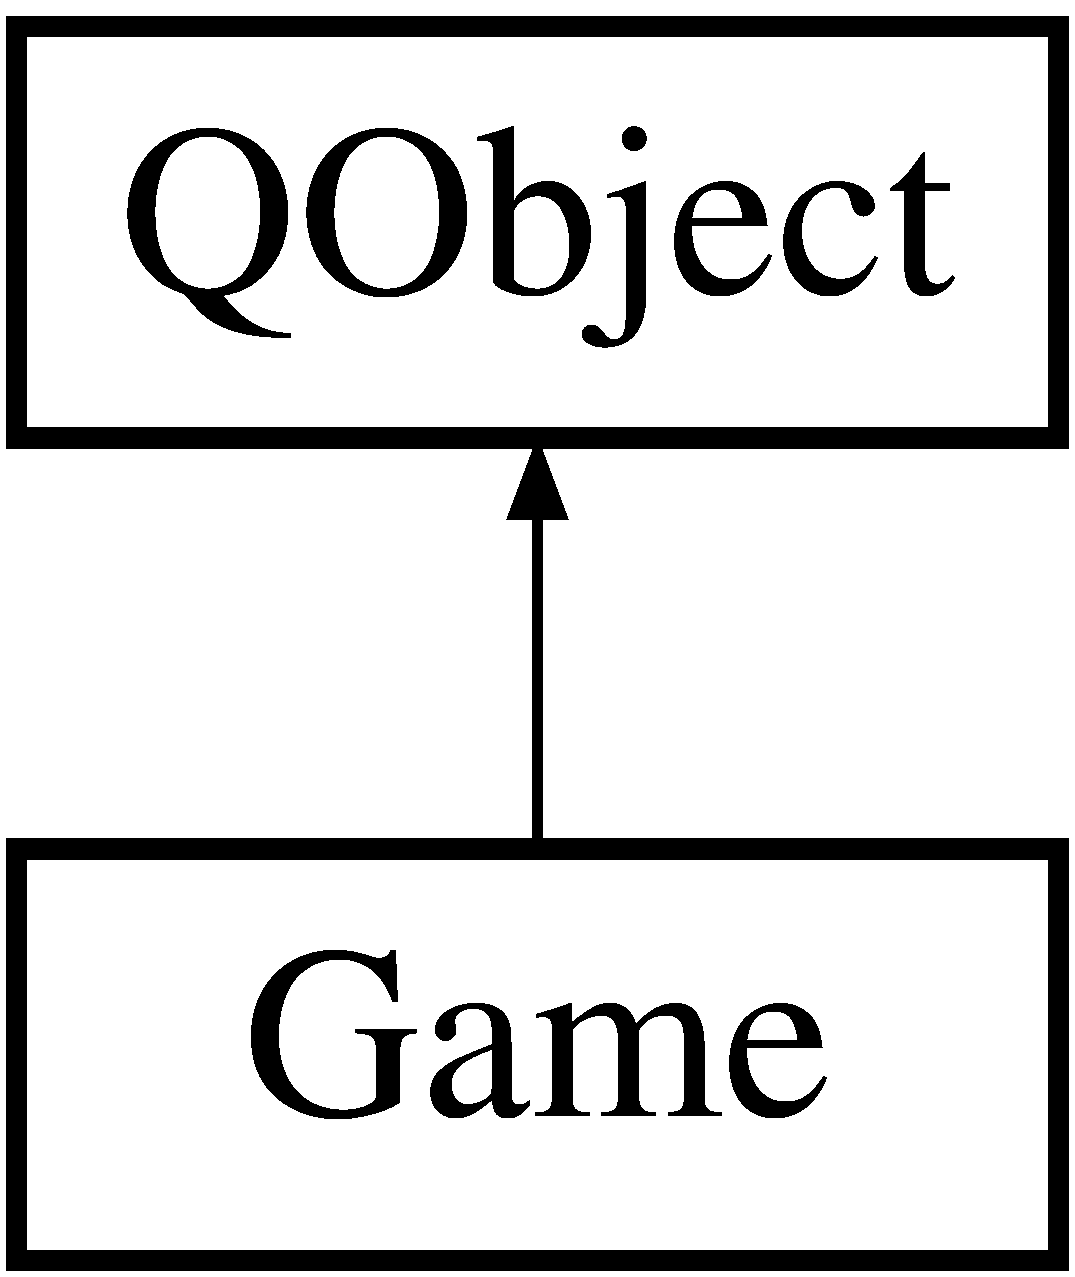
\includegraphics[height=2.000000cm]{class_game}
\end{center}
\end{figure}
\subsection*{Signals}
\begin{DoxyCompactItemize}
\item 
void \hyperlink{class_game_a7c8ac8994a4a829de95544268ada916e}{player\-Changed} ()
\end{DoxyCompactItemize}
\subsection*{Public Member Functions}
\begin{DoxyCompactItemize}
\item 
\hyperlink{class_game_ab1f8c81ce4221a80b7a27320e92ebaed}{Game} (vector$<$ \hyperlink{class_player}{Player} $\ast$ $>$, \hyperlink{class_dictionary}{Dictionary} $\ast$)
\begin{DoxyCompactList}\small\item\em \hyperlink{class_game_ab1f8c81ce4221a80b7a27320e92ebaed}{Game\-::\-Game} Constructor for up to a 4-\/player game. \end{DoxyCompactList}\item 
\hyperlink{class_game_ae3d112ca6e0e55150d2fdbc704474530}{$\sim$\-Game} ()
\begin{DoxyCompactList}\small\item\em \hyperlink{class_game_ae3d112ca6e0e55150d2fdbc704474530}{Game\-::$\sim$\-Game} Destructor. \end{DoxyCompactList}\item 
\hyperlink{class_game}{Game} $\ast$ \hyperlink{class_game_a62edc885b560e752b04fa64c5a481874}{setup} ()
\item 
\hyperlink{class_player}{Player} $\ast$ \hyperlink{class_game_a7cdf3f086fafd3234dba20409e9b98d3}{current\-Player} ()
\begin{DoxyCompactList}\small\item\em \hyperlink{class_game_a7cdf3f086fafd3234dba20409e9b98d3}{Game\-::current\-Player} Gets the current player. \end{DoxyCompactList}\item 
\hyperlink{class_play}{Play} $\ast$ \hyperlink{class_game_acba299674208d186660ed4a88e58d967}{current\-Play} ()
\begin{DoxyCompactList}\small\item\em \hyperlink{class_game_acba299674208d186660ed4a88e58d967}{Game\-::current\-Play} Gets the curret play. \end{DoxyCompactList}\item 
bool \hyperlink{class_game_a6ec161629afa5e24452040bb620eb4bb}{next\-Turn} ()
\begin{DoxyCompactList}\small\item\em \hyperlink{class_game_a6ec161629afa5e24452040bb620eb4bb}{Game\-::next\-Turn} Finalizes the current turn. If a player is an A\-Player, play() is called. \end{DoxyCompactList}\item 
\hyperlink{class_game}{Game} $\ast$ \hyperlink{class_game_a19604b02effa3de3b4157f955c9cea59}{get\-New\-Letters} ()
\end{DoxyCompactItemize}
\subsection*{Public Attributes}
\begin{DoxyCompactItemize}
\item 
\hyperlink{class_dictionary}{Dictionary} $\ast$ \hyperlink{class_game_ac02ac16d33949edb2c83b9c6ce48e596}{dictionary}
\end{DoxyCompactItemize}
\subsection*{Private Attributes}
\begin{DoxyCompactItemize}
\item 
int \hyperlink{class_game_aef6ba37517324fc3469dfa65d6f92d21}{turn}
\item 
\hyperlink{class_letter_pool}{Letter\-Pool} $\ast$ \hyperlink{class_game_ae3b2cb6cd3fd8cf83dc8cd8a6068487a}{pool}
\item 
vector$<$ \hyperlink{class_player}{Player} $\ast$ $>$ \hyperlink{class_game_a8b1b6150488acf6e0d3a222dbf359842}{players}
\item 
vector$<$ \hyperlink{class_play}{Play} $\ast$ $>$ \hyperlink{class_game_a358b65cc87708ae0fe5793bae968971f}{plays}
\item 
int \hyperlink{class_game_a7c03c2f209dfde4ef01c739b050159f6}{num\-Players}
\end{DoxyCompactItemize}
\subsection*{Friends}
\begin{DoxyCompactItemize}
\item 
ostream \& \hyperlink{class_game_a41c0344e76853337b335ed0cb6df12ec}{operator$<$$<$} (ostream \&os, const \hyperlink{class_game}{Game} \&game)
\begin{DoxyCompactList}\small\item\em operator $<$$<$ Overloading the $<$$<$ operator for debugging information \end{DoxyCompactList}\end{DoxyCompactItemize}


\subsection{Detailed Description}
The \hyperlink{class_game}{Game} class Encapsulates a game. 

Definition at line 20 of file game.\-h.



\subsection{Constructor \& Destructor Documentation}
\hypertarget{class_game_ab1f8c81ce4221a80b7a27320e92ebaed}{\index{Game@{Game}!Game@{Game}}
\index{Game@{Game}!Game@{Game}}
\subsubsection[{Game}]{\setlength{\rightskip}{0pt plus 5cm}Game\-::\-Game (
\begin{DoxyParamCaption}
\item[{vector$<$ {\bf Player} $\ast$ $>$}]{players, }
\item[{{\bf Dictionary} $\ast$}]{dictionary}
\end{DoxyParamCaption}
)}}\label{class_game_ab1f8c81ce4221a80b7a27320e92ebaed}


\hyperlink{class_game_ab1f8c81ce4221a80b7a27320e92ebaed}{Game\-::\-Game} Constructor for up to a 4-\/player game. 


\begin{DoxyParams}{Parameters}
{\em players} & The players we are constructive this game for. \\
\hline
{\em dictionary} & The dictionary to use \\
\hline
\end{DoxyParams}


Definition at line 10 of file game.\-cpp.



References current\-Player(), dictionary, next\-Turn(), num\-Players, player\-Changed(), players, plays, pool, and turn.


\begin{DoxyCode}
10                                                          \{
11     this->\hyperlink{class_game_aef6ba37517324fc3469dfa65d6f92d21}{turn} = 0;
12     this->\hyperlink{class_game_ae3b2cb6cd3fd8cf83dc8cd8a6068487a}{pool} = \textcolor{keyword}{new} \hyperlink{class_letter_pool}{LetterPool};
13     this->\hyperlink{class_game_a7c03c2f209dfde4ef01c739b050159f6}{numPlayers} = \hyperlink{class_game_a8b1b6150488acf6e0d3a222dbf359842}{players}.size();
14     this->\hyperlink{class_game_a8b1b6150488acf6e0d3a222dbf359842}{players} = \hyperlink{class_game_a8b1b6150488acf6e0d3a222dbf359842}{players};
15     this->\hyperlink{class_game_a358b65cc87708ae0fe5793bae968971f}{plays}.push\_back(\textcolor{keyword}{new} \hyperlink{class_play}{Play}());
16     this->dictionary = \hyperlink{class_game_ac02ac16d33949edb2c83b9c6ce48e596}{dictionary};
17     \textcolor{keywordflow}{for}(std::vector<Player*>::iterator it = \hyperlink{class_game_a8b1b6150488acf6e0d3a222dbf359842}{players}.begin(); it != 
      \hyperlink{class_game_a8b1b6150488acf6e0d3a222dbf359842}{players}.end(); ++it) \{
18         (*it)->fillLetters(\hyperlink{class_game_ae3b2cb6cd3fd8cf83dc8cd8a6068487a}{pool});
19         assert((*it)->getLetterCount() == 7);
20     \}
21 
22     emit(\hyperlink{class_game_a7c8ac8994a4a829de95544268ada916e}{playerChanged}());
23 
24     \textcolor{keywordflow}{if}(\hyperlink{class_game_a7cdf3f086fafd3234dba20409e9b98d3}{currentPlayer}()->isAIPlayer())\{
25         ((\hyperlink{class_a_i_player}{AIPlayer}*)\hyperlink{class_game_a7cdf3f086fafd3234dba20409e9b98d3}{currentPlayer}())->play(*dictionary, &
      \hyperlink{class_game_a358b65cc87708ae0fe5793bae968971f}{plays}.back());
26         \hyperlink{class_game_a6ec161629afa5e24452040bb620eb4bb}{nextTurn}();
27     \}
28 \}
\end{DoxyCode}
\hypertarget{class_game_ae3d112ca6e0e55150d2fdbc704474530}{\index{Game@{Game}!$\sim$\-Game@{$\sim$\-Game}}
\index{$\sim$\-Game@{$\sim$\-Game}!Game@{Game}}
\subsubsection[{$\sim$\-Game}]{\setlength{\rightskip}{0pt plus 5cm}Game\-::$\sim$\-Game (
\begin{DoxyParamCaption}
{}
\end{DoxyParamCaption}
)}}\label{class_game_ae3d112ca6e0e55150d2fdbc704474530}


\hyperlink{class_game_ae3d112ca6e0e55150d2fdbc704474530}{Game\-::$\sim$\-Game} Destructor. 



Definition at line 57 of file game.\-cpp.



References players.


\begin{DoxyCode}
57            \{
58     \textcolor{keywordflow}{for}(std::vector<Player*>::iterator it = \hyperlink{class_game_a8b1b6150488acf6e0d3a222dbf359842}{players}.begin(); it != 
      \hyperlink{class_game_a8b1b6150488acf6e0d3a222dbf359842}{players}.end(); ++it) \{
59         \textcolor{keywordflow}{if} (*it != NULL)\{
60             (*it)->clearLetters();
61             assert((*it)->getLetterCount() == 0);
62         \}
63     \}
64 \}
\end{DoxyCode}


\subsection{Member Function Documentation}
\hypertarget{class_game_acba299674208d186660ed4a88e58d967}{\index{Game@{Game}!current\-Play@{current\-Play}}
\index{current\-Play@{current\-Play}!Game@{Game}}
\subsubsection[{current\-Play}]{\setlength{\rightskip}{0pt plus 5cm}{\bf Play} $\ast$ Game\-::current\-Play (
\begin{DoxyParamCaption}
{}
\end{DoxyParamCaption}
)}}\label{class_game_acba299674208d186660ed4a88e58d967}


\hyperlink{class_game_acba299674208d186660ed4a88e58d967}{Game\-::current\-Play} Gets the curret play. 

\begin{DoxyReturn}{Returns}
A pointer to the current play 
\end{DoxyReturn}


Definition at line 79 of file game.\-cpp.



References plays.



Referenced by Board\-::move\-Letter\-To\-Board(), next\-Turn(), Board\-::on\-\_\-cancel\-Button\-\_\-clicked(), and Space\-::on\-\_\-clicked().


\begin{DoxyCode}
80 \{
81     \textcolor{keywordflow}{return} \hyperlink{class_game_a358b65cc87708ae0fe5793bae968971f}{plays}.back();
82 \}
\end{DoxyCode}
\hypertarget{class_game_a7cdf3f086fafd3234dba20409e9b98d3}{\index{Game@{Game}!current\-Player@{current\-Player}}
\index{current\-Player@{current\-Player}!Game@{Game}}
\subsubsection[{current\-Player}]{\setlength{\rightskip}{0pt plus 5cm}{\bf Player} $\ast$ Game\-::current\-Player (
\begin{DoxyParamCaption}
{}
\end{DoxyParamCaption}
)}}\label{class_game_a7cdf3f086fafd3234dba20409e9b98d3}


\hyperlink{class_game_a7cdf3f086fafd3234dba20409e9b98d3}{Game\-::current\-Player} Gets the current player. 

\begin{DoxyReturn}{Returns}
A pointer to the current player 
\end{DoxyReturn}


Definition at line 70 of file game.\-cpp.



References num\-Players, players, and turn.



Referenced by Game(), Board\-::move\-Letter\-To\-Board(), next\-Turn(), and Rack\-::refresh().


\begin{DoxyCode}
71 \{
72     \textcolor{keywordflow}{return} \hyperlink{class_game_a8b1b6150488acf6e0d3a222dbf359842}{players}[\hyperlink{class_game_aef6ba37517324fc3469dfa65d6f92d21}{turn} % \hyperlink{class_game_a7c03c2f209dfde4ef01c739b050159f6}{numPlayers}];
73 \}
\end{DoxyCode}
\hypertarget{class_game_a19604b02effa3de3b4157f955c9cea59}{\index{Game@{Game}!get\-New\-Letters@{get\-New\-Letters}}
\index{get\-New\-Letters@{get\-New\-Letters}!Game@{Game}}
\subsubsection[{get\-New\-Letters}]{\setlength{\rightskip}{0pt plus 5cm}{\bf Game}$\ast$ Game\-::get\-New\-Letters (
\begin{DoxyParamCaption}
{}
\end{DoxyParamCaption}
)}}\label{class_game_a19604b02effa3de3b4157f955c9cea59}
\hypertarget{class_game_a6ec161629afa5e24452040bb620eb4bb}{\index{Game@{Game}!next\-Turn@{next\-Turn}}
\index{next\-Turn@{next\-Turn}!Game@{Game}}
\subsubsection[{next\-Turn}]{\setlength{\rightskip}{0pt plus 5cm}bool Game\-::next\-Turn (
\begin{DoxyParamCaption}
{}
\end{DoxyParamCaption}
)}}\label{class_game_a6ec161629afa5e24452040bb620eb4bb}


\hyperlink{class_game_a6ec161629afa5e24452040bb620eb4bb}{Game\-::next\-Turn} Finalizes the current turn. If a player is an A\-Player, play() is called. 

\begin{DoxyReturn}{Returns}
this 
\end{DoxyReturn}


Definition at line 35 of file game.\-cpp.



References Player\-::add\-Score(), current\-Play(), current\-Player(), dictionary, Play\-::finalize\-Moves(), Board\-::get\-Board(), Player\-::get\-New\-Letters(), Rack\-::get\-Rack(), player\-Changed(), plays, pool, Rack\-::refresh(), and turn.



Referenced by Game(), Board\-::on\-\_\-pass\-Button\-\_\-clicked(), and Board\-::on\-\_\-play\-Button\-\_\-clicked().


\begin{DoxyCode}
36 \{
37     \hyperlink{class_game_a7cdf3f086fafd3234dba20409e9b98d3}{currentPlayer}()->\hyperlink{class_player_aa5bead96a6eb9cc33fbc086662621caf}{addScore}(\hyperlink{class_board_ae30e802b1d83309fc95e695b5b3df338}{Board::getBoard}()->score(
      \hyperlink{class_game_a358b65cc87708ae0fe5793bae968971f}{plays}.back()));
38     \hyperlink{class_game_a7cdf3f086fafd3234dba20409e9b98d3}{currentPlayer}()->\hyperlink{class_player_a78086401345079616a422c25cb780ecb}{getNewLetters}(\hyperlink{class_game_ae3b2cb6cd3fd8cf83dc8cd8a6068487a}{pool});
39     \hyperlink{class_game_acba299674208d186660ed4a88e58d967}{currentPlay}()->\hyperlink{class_play_a02fbcafed804466c41fd78e8eef8ca16}{finalizeMoves}();
40     \hyperlink{class_game_aef6ba37517324fc3469dfa65d6f92d21}{turn} = \hyperlink{class_game_aef6ba37517324fc3469dfa65d6f92d21}{turn} + 1;
41     \hyperlink{class_rack_aa48de650c15bda8267451d84caf6ea3f}{Rack::getRack}()->\hyperlink{class_rack_ae1b5a6e15cb1ebe299356959b6a8d641}{refresh}(\textcolor{keyword}{this});
42     emit(\hyperlink{class_game_a7c8ac8994a4a829de95544268ada916e}{playerChanged}());
43 
44     \hyperlink{class_game_a358b65cc87708ae0fe5793bae968971f}{plays}.push\_back(\textcolor{keyword}{new} \hyperlink{class_play}{Play}());
45 
46     \textcolor{keywordflow}{if}(\hyperlink{class_game_a7cdf3f086fafd3234dba20409e9b98d3}{currentPlayer}()->isAIPlayer() && \hyperlink{class_game_a7cdf3f086fafd3234dba20409e9b98d3}{currentPlayer}()->getLetterCount() > 0)\{
47         ((\hyperlink{class_a_i_player}{AIPlayer}*)\hyperlink{class_game_a7cdf3f086fafd3234dba20409e9b98d3}{currentPlayer}())->play(*\hyperlink{class_game_ac02ac16d33949edb2c83b9c6ce48e596}{dictionary}, &
      \hyperlink{class_game_a358b65cc87708ae0fe5793bae968971f}{plays}.back());
48         \hyperlink{class_game_a6ec161629afa5e24452040bb620eb4bb}{nextTurn}();
49     \}
50 
51     \textcolor{keywordflow}{return} \textcolor{keyword}{true};
52 \}
\end{DoxyCode}
\hypertarget{class_game_a7c8ac8994a4a829de95544268ada916e}{\index{Game@{Game}!player\-Changed@{player\-Changed}}
\index{player\-Changed@{player\-Changed}!Game@{Game}}
\subsubsection[{player\-Changed}]{\setlength{\rightskip}{0pt plus 5cm}void Game\-::player\-Changed (
\begin{DoxyParamCaption}
{}
\end{DoxyParamCaption}
)\hspace{0.3cm}{\ttfamily [signal]}}}\label{class_game_a7c8ac8994a4a829de95544268ada916e}


Referenced by Game(), and next\-Turn().

\hypertarget{class_game_a62edc885b560e752b04fa64c5a481874}{\index{Game@{Game}!setup@{setup}}
\index{setup@{setup}!Game@{Game}}
\subsubsection[{setup}]{\setlength{\rightskip}{0pt plus 5cm}{\bf Game}$\ast$ Game\-::setup (
\begin{DoxyParamCaption}
{}
\end{DoxyParamCaption}
)}}\label{class_game_a62edc885b560e752b04fa64c5a481874}


\subsection{Friends And Related Function Documentation}
\hypertarget{class_game_a41c0344e76853337b335ed0cb6df12ec}{\index{Game@{Game}!operator$<$$<$@{operator$<$$<$}}
\index{operator$<$$<$@{operator$<$$<$}!Game@{Game}}
\subsubsection[{operator$<$$<$}]{\setlength{\rightskip}{0pt plus 5cm}ostream\& operator$<$$<$ (
\begin{DoxyParamCaption}
\item[{ostream \&}]{os, }
\item[{const {\bf Game} \&}]{game}
\end{DoxyParamCaption}
)\hspace{0.3cm}{\ttfamily [friend]}}}\label{class_game_a41c0344e76853337b335ed0cb6df12ec}


operator $<$$<$ Overloading the $<$$<$ operator for debugging information 


\begin{DoxyParams}{Parameters}
{\em os} & The output stream \\
\hline
{\em game} & The game object \\
\hline
\end{DoxyParams}
\begin{DoxyReturn}{Returns}
The modified output stream 
\end{DoxyReturn}


Definition at line 90 of file game.\-cpp.


\begin{DoxyCode}
90                                                    \{
91     os << \textcolor{stringliteral}{"This is a "} << game.\hyperlink{class_game_a7c03c2f209dfde4ef01c739b050159f6}{numPlayers} << \textcolor{stringliteral}{" player game."} << endl;
92     os << *(\hyperlink{class_board_ae30e802b1d83309fc95e695b5b3df338}{Board::getBoard}());
93     \textcolor{keywordflow}{return} os;
94 \}
\end{DoxyCode}


\subsection{Member Data Documentation}
\hypertarget{class_game_ac02ac16d33949edb2c83b9c6ce48e596}{\index{Game@{Game}!dictionary@{dictionary}}
\index{dictionary@{dictionary}!Game@{Game}}
\subsubsection[{dictionary}]{\setlength{\rightskip}{0pt plus 5cm}{\bf Dictionary}$\ast$ Game\-::dictionary}}\label{class_game_ac02ac16d33949edb2c83b9c6ce48e596}
The \hyperlink{class_dictionary}{Dictionary} 

Definition at line 31 of file game.\-h.



Referenced by Game(), next\-Turn(), Board\-::validate\-Word\-Horizontal(), and Board\-::validate\-Word\-Vertical().

\hypertarget{class_game_a7c03c2f209dfde4ef01c739b050159f6}{\index{Game@{Game}!num\-Players@{num\-Players}}
\index{num\-Players@{num\-Players}!Game@{Game}}
\subsubsection[{num\-Players}]{\setlength{\rightskip}{0pt plus 5cm}int Game\-::num\-Players\hspace{0.3cm}{\ttfamily [private]}}}\label{class_game_a7c03c2f209dfde4ef01c739b050159f6}
The number of players 

Definition at line 28 of file game.\-h.



Referenced by current\-Player(), Game(), and operator$<$$<$().

\hypertarget{class_game_a8b1b6150488acf6e0d3a222dbf359842}{\index{Game@{Game}!players@{players}}
\index{players@{players}!Game@{Game}}
\subsubsection[{players}]{\setlength{\rightskip}{0pt plus 5cm}vector$<${\bf Player}$\ast$$>$ Game\-::players\hspace{0.3cm}{\ttfamily [private]}}}\label{class_game_a8b1b6150488acf6e0d3a222dbf359842}
The container for the Players 

Definition at line 26 of file game.\-h.



Referenced by current\-Player(), Game(), and $\sim$\-Game().

\hypertarget{class_game_a358b65cc87708ae0fe5793bae968971f}{\index{Game@{Game}!plays@{plays}}
\index{plays@{plays}!Game@{Game}}
\subsubsection[{plays}]{\setlength{\rightskip}{0pt plus 5cm}vector$<${\bf Play}$\ast$$>$ Game\-::plays\hspace{0.3cm}{\ttfamily [private]}}}\label{class_game_a358b65cc87708ae0fe5793bae968971f}
The container for the Plays 

Definition at line 27 of file game.\-h.



Referenced by current\-Play(), Game(), and next\-Turn().

\hypertarget{class_game_ae3b2cb6cd3fd8cf83dc8cd8a6068487a}{\index{Game@{Game}!pool@{pool}}
\index{pool@{pool}!Game@{Game}}
\subsubsection[{pool}]{\setlength{\rightskip}{0pt plus 5cm}{\bf Letter\-Pool}$\ast$ Game\-::pool\hspace{0.3cm}{\ttfamily [private]}}}\label{class_game_ae3b2cb6cd3fd8cf83dc8cd8a6068487a}
The pool of letters 

Definition at line 25 of file game.\-h.



Referenced by Game(), and next\-Turn().

\hypertarget{class_game_aef6ba37517324fc3469dfa65d6f92d21}{\index{Game@{Game}!turn@{turn}}
\index{turn@{turn}!Game@{Game}}
\subsubsection[{turn}]{\setlength{\rightskip}{0pt plus 5cm}int Game\-::turn\hspace{0.3cm}{\ttfamily [private]}}}\label{class_game_aef6ba37517324fc3469dfa65d6f92d21}
The number of the turn 

Definition at line 24 of file game.\-h.



Referenced by current\-Player(), Game(), and next\-Turn().



The documentation for this class was generated from the following files\-:\begin{DoxyCompactItemize}
\item 
Scrabble/\hyperlink{game_8h}{game.\-h}\item 
Scrabble/\hyperlink{game_8cpp}{game.\-cpp}\end{DoxyCompactItemize}

\hypertarget{class_human_player}{\section{Human\-Player Class Reference}
\label{class_human_player}\index{Human\-Player@{Human\-Player}}
}


The \hyperlink{class_human_player}{Human\-Player} class Human playable \hyperlink{class_player}{Player}.  




{\ttfamily \#include $<$humanplayer.\-h$>$}

Inheritance diagram for Human\-Player\-:\begin{figure}[H]
\begin{center}
\leavevmode
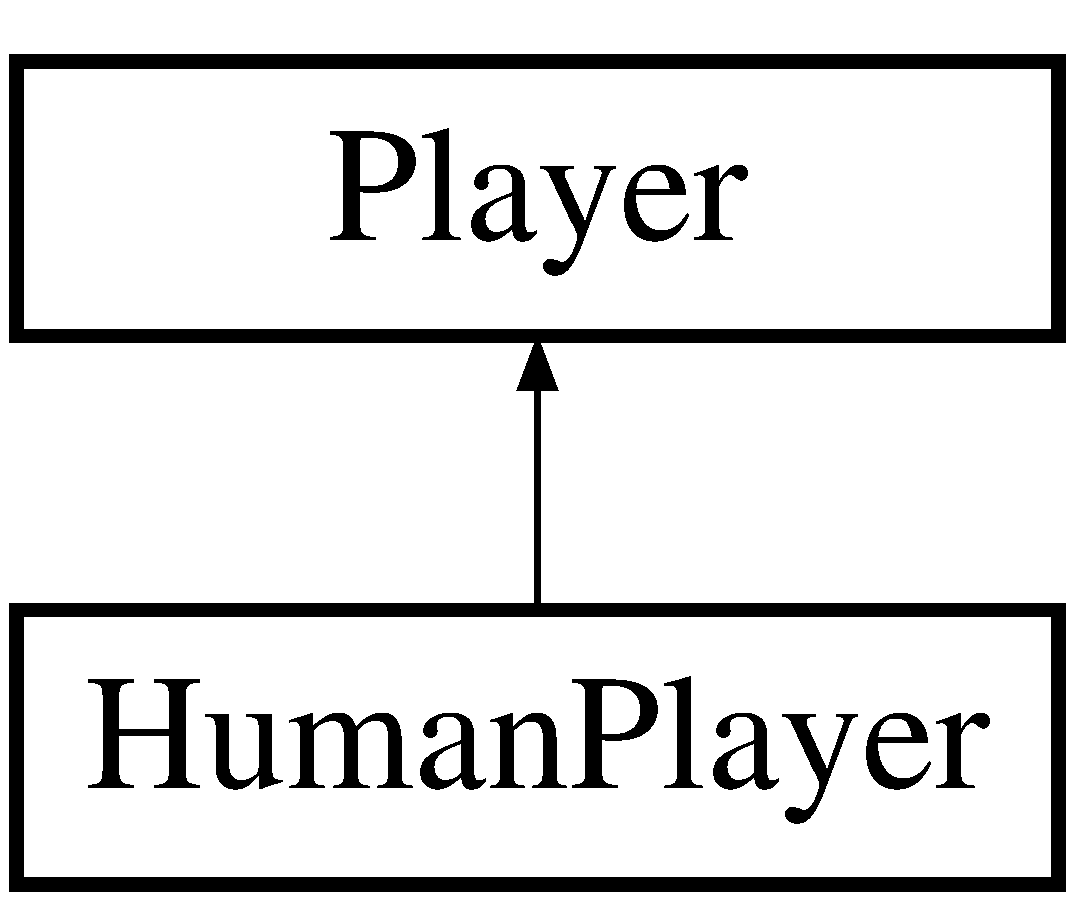
\includegraphics[height=2.000000cm]{class_human_player}
\end{center}
\end{figure}
\subsection*{Public Member Functions}
\begin{DoxyCompactItemize}
\item 
\hyperlink{class_human_player_aca695b2fb575e41bf7f015387c6eb52a}{Human\-Player} (Q\-String s)
\item 
\hyperlink{class_human_player_abdeb9d120fc74c8d82ec0c688883f16f}{$\sim$\-Human\-Player} ()
\begin{DoxyCompactList}\small\item\em \hyperlink{class_human_player_abdeb9d120fc74c8d82ec0c688883f16f}{Human\-Player\-::$\sim$\-Human\-Player} Destructor. \end{DoxyCompactList}\item 
\hyperlink{class_play}{Play} $\ast$ \hyperlink{class_human_player_acd62878a6a3612685aca20853bbca3e2}{play} (\hyperlink{class_board}{Board} $\ast$board)
\item 
virtual bool \hyperlink{class_human_player_aff784db8904c5f8c13bd88847f631188}{is\-Human\-Player} ()
\begin{DoxyCompactList}\small\item\em \hyperlink{class_human_player_aff784db8904c5f8c13bd88847f631188}{Human\-Player\-::is\-Human\-Player}. \end{DoxyCompactList}\end{DoxyCompactItemize}
\subsection*{Additional Inherited Members}


\subsection{Detailed Description}
The \hyperlink{class_human_player}{Human\-Player} class Human playable \hyperlink{class_player}{Player}. 

Definition at line 8 of file humanplayer.\-h.



\subsection{Constructor \& Destructor Documentation}
\hypertarget{class_human_player_aca695b2fb575e41bf7f015387c6eb52a}{\index{Human\-Player@{Human\-Player}!Human\-Player@{Human\-Player}}
\index{Human\-Player@{Human\-Player}!HumanPlayer@{Human\-Player}}
\subsubsection[{Human\-Player}]{\setlength{\rightskip}{0pt plus 5cm}Human\-Player\-::\-Human\-Player (
\begin{DoxyParamCaption}
\item[{Q\-String}]{s}
\end{DoxyParamCaption}
)\hspace{0.3cm}{\ttfamily [inline]}}}\label{class_human_player_aca695b2fb575e41bf7f015387c6eb52a}


Definition at line 10 of file humanplayer.\-h.


\begin{DoxyCode}
10 : \hyperlink{class_player_ad079d0b82440f180a6698ff62f1dc1be}{Player}(s) \{\}
\end{DoxyCode}
\hypertarget{class_human_player_abdeb9d120fc74c8d82ec0c688883f16f}{\index{Human\-Player@{Human\-Player}!$\sim$\-Human\-Player@{$\sim$\-Human\-Player}}
\index{$\sim$\-Human\-Player@{$\sim$\-Human\-Player}!HumanPlayer@{Human\-Player}}
\subsubsection[{$\sim$\-Human\-Player}]{\setlength{\rightskip}{0pt plus 5cm}Human\-Player\-::$\sim$\-Human\-Player (
\begin{DoxyParamCaption}
{}
\end{DoxyParamCaption}
)}}\label{class_human_player_abdeb9d120fc74c8d82ec0c688883f16f}


\hyperlink{class_human_player_abdeb9d120fc74c8d82ec0c688883f16f}{Human\-Player\-::$\sim$\-Human\-Player} Destructor. 



Definition at line 6 of file humanplayer.\-cpp.



References Player\-::letters.


\begin{DoxyCode}
6                           \{
7     \textcolor{keywordflow}{while} (!\hyperlink{class_player_abd40dc8f6d524bd1331a8133e9bb8902}{letters}.empty())\{
8         \textcolor{keyword}{delete} \hyperlink{class_player_abd40dc8f6d524bd1331a8133e9bb8902}{letters}.back();
9         \hyperlink{class_player_abd40dc8f6d524bd1331a8133e9bb8902}{letters}.pop\_back();
10     \}
11 \}
\end{DoxyCode}


\subsection{Member Function Documentation}
\hypertarget{class_human_player_aff784db8904c5f8c13bd88847f631188}{\index{Human\-Player@{Human\-Player}!is\-Human\-Player@{is\-Human\-Player}}
\index{is\-Human\-Player@{is\-Human\-Player}!HumanPlayer@{Human\-Player}}
\subsubsection[{is\-Human\-Player}]{\setlength{\rightskip}{0pt plus 5cm}bool Human\-Player\-::is\-Human\-Player (
\begin{DoxyParamCaption}
{}
\end{DoxyParamCaption}
)\hspace{0.3cm}{\ttfamily [virtual]}}}\label{class_human_player_aff784db8904c5f8c13bd88847f631188}


\hyperlink{class_human_player_aff784db8904c5f8c13bd88847f631188}{Human\-Player\-::is\-Human\-Player}. 

This is an overloaded member function, provided for convenience. It differs from the above function only in what argument(s) it accepts. \begin{DoxyReturn}{Returns}
True if player is a human, false otherwise 
\end{DoxyReturn}


Reimplemented from \hyperlink{class_player_adeb8d6fe962f9bf002281f7fe1321cff}{Player}.



Definition at line 18 of file humanplayer.\-cpp.


\begin{DoxyCode}
18                                \{
19     \textcolor{keywordflow}{return} \textcolor{keyword}{true};
20 \}
\end{DoxyCode}
\hypertarget{class_human_player_acd62878a6a3612685aca20853bbca3e2}{\index{Human\-Player@{Human\-Player}!play@{play}}
\index{play@{play}!HumanPlayer@{Human\-Player}}
\subsubsection[{play}]{\setlength{\rightskip}{0pt plus 5cm}{\bf Play}$\ast$ Human\-Player\-::play (
\begin{DoxyParamCaption}
\item[{{\bf Board} $\ast$}]{board}
\end{DoxyParamCaption}
)}}\label{class_human_player_acd62878a6a3612685aca20853bbca3e2}


The documentation for this class was generated from the following files\-:\begin{DoxyCompactItemize}
\item 
Scrabble/\hyperlink{humanplayer_8h}{humanplayer.\-h}\item 
Scrabble/\hyperlink{humanplayer_8cpp}{humanplayer.\-cpp}\end{DoxyCompactItemize}

\hypertarget{class_letter}{\section{Letter Class Reference}
\label{class_letter}\index{Letter@{Letter}}
}


The \hyperlink{class_letter}{Letter} class Encapsulates a \hyperlink{class_letter}{Letter} (or Tile)  




{\ttfamily \#include $<$letter.\-h$>$}

\subsection*{Public Member Functions}
\begin{DoxyCompactItemize}
\item 
\hyperlink{class_letter_aeaf51ffac3bafca1b1cc504381a6152f}{Letter} (Q\-Char)
\begin{DoxyCompactList}\small\item\em \hyperlink{class_letter_aeaf51ffac3bafca1b1cc504381a6152f}{Letter\-::\-Letter} Constructor. \end{DoxyCompactList}\item 
unsigned int \hyperlink{class_letter_a5980d43229d58bfab9fdb20f25e88e9e}{get\-Value} ()
\begin{DoxyCompactList}\small\item\em \hyperlink{class_letter_a5980d43229d58bfab9fdb20f25e88e9e}{Letter\-::get\-Value} Getter for value. \end{DoxyCompactList}\item 
void \hyperlink{class_letter_a9f2f4067a9fd386366273af73fac70e5}{set\-Letter} (Q\-Char)
\begin{DoxyCompactList}\small\item\em Letter\-::set\-Value Setter for value, only for wildcards. \end{DoxyCompactList}\item 
bool \hyperlink{class_letter_a7e6053ff071263d8bc876d31101ea235}{is\-A\-Match} (Q\-Char)
\begin{DoxyCompactList}\small\item\em \hyperlink{class_letter_a7e6053ff071263d8bc876d31101ea235}{Letter\-::is\-A\-Match} Tests if a character is a match to this letter. \end{DoxyCompactList}\item 
bool \hyperlink{class_letter_aa0c05656947c35b032b20b7260f463ba}{is\-Wildcard} ()
\begin{DoxyCompactList}\small\item\em \hyperlink{class_letter_aa0c05656947c35b032b20b7260f463ba}{Letter\-::is\-Wildcard}. \end{DoxyCompactList}\item 
Q\-Char $\ast$ \hyperlink{class_letter_aa7fb6547b5ceefef8d0a014ab0a80d08}{as\-Q\-Char\-Ptr} ()
\begin{DoxyCompactList}\small\item\em Letter\-::get\-Letter Getter for this letter. \end{DoxyCompactList}\end{DoxyCompactItemize}
\subsection*{Private Attributes}
\begin{DoxyCompactItemize}
\item 
Q\-Char \hyperlink{class_letter_a430f7ba15c252da3874f641422090fbd}{letter}
\item 
unsigned int \hyperlink{class_letter_a5c6b1982acd4967eec202c562be7bc8f}{value}
\item 
bool \hyperlink{class_letter_a6c34169c5f139924fb14154391bf1925}{wildcard}
\end{DoxyCompactItemize}
\subsection*{Friends}
\begin{DoxyCompactItemize}
\item 
ostream \& \hyperlink{class_letter_a90f2b9e82cfd5e6c60087fb6c1f92937}{operator$<$$<$} (ostream \&os, const \hyperlink{class_letter}{Letter} \&\hyperlink{class_letter_a430f7ba15c252da3874f641422090fbd}{letter})
\begin{DoxyCompactList}\small\item\em operator $<$$<$ Overloaded ostream operator \end{DoxyCompactList}\end{DoxyCompactItemize}


\subsection{Detailed Description}
The \hyperlink{class_letter}{Letter} class Encapsulates a \hyperlink{class_letter}{Letter} (or Tile) 

Definition at line 11 of file letter.\-h.



\subsection{Constructor \& Destructor Documentation}
\hypertarget{class_letter_aeaf51ffac3bafca1b1cc504381a6152f}{\index{Letter@{Letter}!Letter@{Letter}}
\index{Letter@{Letter}!Letter@{Letter}}
\subsubsection[{Letter}]{\setlength{\rightskip}{0pt plus 5cm}Letter\-::\-Letter (
\begin{DoxyParamCaption}
\item[{Q\-Char}]{letter}
\end{DoxyParamCaption}
)}}\label{class_letter_aeaf51ffac3bafca1b1cc504381a6152f}


\hyperlink{class_letter_aeaf51ffac3bafca1b1cc504381a6152f}{Letter\-::\-Letter} Constructor. 


\begin{DoxyParams}{Parameters}
{\em letter} & The letter to set \\
\hline
\end{DoxyParams}


Definition at line 8 of file letter.\-cpp.



References value, and wildcard.


\begin{DoxyCode}
8                           \{
9 
10     \hyperlink{class_letter_a6c34169c5f139924fb14154391bf1925}{wildcard} = \textcolor{keyword}{false};
11     this->\hyperlink{class_letter_a430f7ba15c252da3874f641422090fbd}{letter} = \hyperlink{class_letter_a430f7ba15c252da3874f641422090fbd}{letter}.toLower();
12     \textcolor{keywordflow}{switch} (this->\hyperlink{class_letter_a430f7ba15c252da3874f641422090fbd}{letter}.toLatin1()) \{
13     \textcolor{keywordflow}{case}(\textcolor{charliteral}{'d'}):
14     \textcolor{keywordflow}{case}(\textcolor{charliteral}{'g'}):
15         this->\hyperlink{class_letter_a5c6b1982acd4967eec202c562be7bc8f}{value} = 2;
16         \textcolor{keywordflow}{break};
17     \textcolor{keywordflow}{case}(\textcolor{charliteral}{'b'}):
18     \textcolor{keywordflow}{case}(\textcolor{charliteral}{'c'}):
19     \textcolor{keywordflow}{case}(\textcolor{charliteral}{'m'}):
20     \textcolor{keywordflow}{case}(\textcolor{charliteral}{'p'}):
21         this->\hyperlink{class_letter_a5c6b1982acd4967eec202c562be7bc8f}{value} = 3;
22         \textcolor{keywordflow}{break};
23     \textcolor{keywordflow}{case}(\textcolor{charliteral}{'f'}):
24     \textcolor{keywordflow}{case}(\textcolor{charliteral}{'h'}):
25     \textcolor{keywordflow}{case}(\textcolor{charliteral}{'v'}):
26     \textcolor{keywordflow}{case}(\textcolor{charliteral}{'w'}):
27     \textcolor{keywordflow}{case}(\textcolor{charliteral}{'y'}):
28        this->\hyperlink{class_letter_a5c6b1982acd4967eec202c562be7bc8f}{value} = 4;
29        \textcolor{keywordflow}{break};
30     \textcolor{keywordflow}{case}(\textcolor{charliteral}{'k'}):
31         this->\hyperlink{class_letter_a5c6b1982acd4967eec202c562be7bc8f}{value} = 5;
32         \textcolor{keywordflow}{break};
33     \textcolor{keywordflow}{case}(\textcolor{charliteral}{'j'}):
34     \textcolor{keywordflow}{case}(\textcolor{charliteral}{'x'}):
35         this->\hyperlink{class_letter_a5c6b1982acd4967eec202c562be7bc8f}{value} = 8;
36         \textcolor{keywordflow}{break};
37     \textcolor{keywordflow}{case}(\textcolor{charliteral}{'q'}):
38     \textcolor{keywordflow}{case}(\textcolor{charliteral}{'z'}):
39         this->\hyperlink{class_letter_a5c6b1982acd4967eec202c562be7bc8f}{value} = 10;
40         \textcolor{keywordflow}{break};
41     \textcolor{keywordflow}{case}(\textcolor{charliteral}{' '}):
42         this->\hyperlink{class_letter_a5c6b1982acd4967eec202c562be7bc8f}{value} = 0;
43         \hyperlink{class_letter_a6c34169c5f139924fb14154391bf1925}{wildcard} = \textcolor{keyword}{true};
44         \textcolor{keywordflow}{break};
45     \textcolor{keywordflow}{default}:
46         this->\hyperlink{class_letter_a5c6b1982acd4967eec202c562be7bc8f}{value} = 1;
47         \textcolor{keywordflow}{break};
48     \}
49 \}
\end{DoxyCode}


\subsection{Member Function Documentation}
\hypertarget{class_letter_aa7fb6547b5ceefef8d0a014ab0a80d08}{\index{Letter@{Letter}!as\-Q\-Char\-Ptr@{as\-Q\-Char\-Ptr}}
\index{as\-Q\-Char\-Ptr@{as\-Q\-Char\-Ptr}!Letter@{Letter}}
\subsubsection[{as\-Q\-Char\-Ptr}]{\setlength{\rightskip}{0pt plus 5cm}Q\-Char $\ast$ Letter\-::as\-Q\-Char\-Ptr (
\begin{DoxyParamCaption}
{}
\end{DoxyParamCaption}
)}}\label{class_letter_aa7fb6547b5ceefef8d0a014ab0a80d08}


Letter\-::get\-Letter Getter for this letter. 

\begin{DoxyReturn}{Returns}
this 
\end{DoxyReturn}


Definition at line 94 of file letter.\-cpp.



References letter.



Referenced by A\-I\-Player\-::\-\_\-assist\-\_\-ai\-\_\-search(), Play\-::get\-Char\-Array(), Space\-::on\-\_\-clicked(), operator$<$$<$(), Space\-::set\-Letter(), Play\-::validate\-\_\-down(), Play\-::validate\-\_\-right(), Board\-::validate\-Word\-Horizontal(), and Board\-::validate\-Word\-Vertical().


\begin{DoxyCode}
94                          \{
95     \textcolor{keywordflow}{return} &(this->\hyperlink{class_letter_a430f7ba15c252da3874f641422090fbd}{letter});
96 \}
\end{DoxyCode}
\hypertarget{class_letter_a5980d43229d58bfab9fdb20f25e88e9e}{\index{Letter@{Letter}!get\-Value@{get\-Value}}
\index{get\-Value@{get\-Value}!Letter@{Letter}}
\subsubsection[{get\-Value}]{\setlength{\rightskip}{0pt plus 5cm}unsigned int Letter\-::get\-Value (
\begin{DoxyParamCaption}
{}
\end{DoxyParamCaption}
)}}\label{class_letter_a5980d43229d58bfab9fdb20f25e88e9e}


\hyperlink{class_letter_a5980d43229d58bfab9fdb20f25e88e9e}{Letter\-::get\-Value} Getter for value. 

\begin{DoxyReturn}{Returns}
value 
\end{DoxyReturn}


Definition at line 55 of file letter.\-cpp.



References value.



Referenced by Space\-::get\-Value(), Board\-::score\-Horizontal\-Word(), Board\-::score\-Vertical\-Word(), and Space\-::set\-Letter().


\begin{DoxyCode}
55                              \{
56     \textcolor{keywordflow}{return} (this->\hyperlink{class_letter_a5c6b1982acd4967eec202c562be7bc8f}{value});
57 \}
\end{DoxyCode}
\hypertarget{class_letter_a7e6053ff071263d8bc876d31101ea235}{\index{Letter@{Letter}!is\-A\-Match@{is\-A\-Match}}
\index{is\-A\-Match@{is\-A\-Match}!Letter@{Letter}}
\subsubsection[{is\-A\-Match}]{\setlength{\rightskip}{0pt plus 5cm}bool Letter\-::is\-A\-Match (
\begin{DoxyParamCaption}
\item[{Q\-Char}]{c}
\end{DoxyParamCaption}
)}}\label{class_letter_a7e6053ff071263d8bc876d31101ea235}


\hyperlink{class_letter_a7e6053ff071263d8bc876d31101ea235}{Letter\-::is\-A\-Match} Tests if a character is a match to this letter. 


\begin{DoxyParams}{Parameters}
{\em c} & The char to compare \\
\hline
\end{DoxyParams}
\begin{DoxyReturn}{Returns}
True if the character is a match, false otherwise 
\end{DoxyReturn}


Definition at line 86 of file letter.\-cpp.



References letter.



Referenced by Space\-::on\-\_\-clicked().


\begin{DoxyCode}
86                             \{
87     \textcolor{keywordflow}{return} this->\hyperlink{class_letter_a430f7ba15c252da3874f641422090fbd}{letter} == c;
88 \}
\end{DoxyCode}
\hypertarget{class_letter_aa0c05656947c35b032b20b7260f463ba}{\index{Letter@{Letter}!is\-Wildcard@{is\-Wildcard}}
\index{is\-Wildcard@{is\-Wildcard}!Letter@{Letter}}
\subsubsection[{is\-Wildcard}]{\setlength{\rightskip}{0pt plus 5cm}bool Letter\-::is\-Wildcard (
\begin{DoxyParamCaption}
{}
\end{DoxyParamCaption}
)}}\label{class_letter_aa0c05656947c35b032b20b7260f463ba}


\hyperlink{class_letter_aa0c05656947c35b032b20b7260f463ba}{Letter\-::is\-Wildcard}. 

\begin{DoxyReturn}{Returns}

\end{DoxyReturn}


Definition at line 75 of file letter.\-cpp.



References wildcard.



Referenced by Space\-::on\-\_\-clicked().


\begin{DoxyCode}
76 \{
77     \textcolor{keywordflow}{return} \hyperlink{class_letter_a6c34169c5f139924fb14154391bf1925}{wildcard};
78 \}
\end{DoxyCode}
\hypertarget{class_letter_a9f2f4067a9fd386366273af73fac70e5}{\index{Letter@{Letter}!set\-Letter@{set\-Letter}}
\index{set\-Letter@{set\-Letter}!Letter@{Letter}}
\subsubsection[{set\-Letter}]{\setlength{\rightskip}{0pt plus 5cm}void Letter\-::set\-Letter (
\begin{DoxyParamCaption}
\item[{Q\-Char}]{c}
\end{DoxyParamCaption}
)}}\label{class_letter_a9f2f4067a9fd386366273af73fac70e5}


Letter\-::set\-Value Setter for value, only for wildcards. 


\begin{DoxyParams}{Parameters}
{\em c} & The value to set \\
\hline
\end{DoxyParams}
\begin{DoxyReturn}{Returns}
this 
\end{DoxyReturn}


Definition at line 64 of file letter.\-cpp.



References letter, and wildcard.



Referenced by Space\-::on\-\_\-clicked().


\begin{DoxyCode}
65 \{
66     \textcolor{keywordflow}{if} (\hyperlink{class_letter_a6c34169c5f139924fb14154391bf1925}{wildcard})\{
67         \hyperlink{class_letter_a430f7ba15c252da3874f641422090fbd}{letter} = c;
68     \}
69 \}
\end{DoxyCode}


\subsection{Friends And Related Function Documentation}
\hypertarget{class_letter_a90f2b9e82cfd5e6c60087fb6c1f92937}{\index{Letter@{Letter}!operator$<$$<$@{operator$<$$<$}}
\index{operator$<$$<$@{operator$<$$<$}!Letter@{Letter}}
\subsubsection[{operator$<$$<$}]{\setlength{\rightskip}{0pt plus 5cm}ostream\& operator$<$$<$ (
\begin{DoxyParamCaption}
\item[{ostream \&}]{os, }
\item[{const {\bf Letter} \&}]{letter}
\end{DoxyParamCaption}
)\hspace{0.3cm}{\ttfamily [friend]}}}\label{class_letter_a90f2b9e82cfd5e6c60087fb6c1f92937}


operator $<$$<$ Overloaded ostream operator 


\begin{DoxyParams}{Parameters}
{\em os} & The ostream \\
\hline
{\em letter} & The letter \\
\hline
\end{DoxyParams}
\begin{DoxyReturn}{Returns}
The modified ostream 
\end{DoxyReturn}


Definition at line 104 of file letter.\-cpp.


\begin{DoxyCode}
104                                                        \{
105     os << letter.\hyperlink{class_letter_a430f7ba15c252da3874f641422090fbd}{letter}.toLatin1();
106     \textcolor{keywordflow}{return} os;
107 \}
\end{DoxyCode}


\subsection{Member Data Documentation}
\hypertarget{class_letter_a430f7ba15c252da3874f641422090fbd}{\index{Letter@{Letter}!letter@{letter}}
\index{letter@{letter}!Letter@{Letter}}
\subsubsection[{letter}]{\setlength{\rightskip}{0pt plus 5cm}Q\-Char Letter\-::letter\hspace{0.3cm}{\ttfamily [private]}}}\label{class_letter_a430f7ba15c252da3874f641422090fbd}
The letter assigned to this tile 

Definition at line 13 of file letter.\-h.



Referenced by as\-Q\-Char\-Ptr(), is\-A\-Match(), operator$<$$<$(), and set\-Letter().

\hypertarget{class_letter_a5c6b1982acd4967eec202c562be7bc8f}{\index{Letter@{Letter}!value@{value}}
\index{value@{value}!Letter@{Letter}}
\subsubsection[{value}]{\setlength{\rightskip}{0pt plus 5cm}unsigned int Letter\-::value\hspace{0.3cm}{\ttfamily [private]}}}\label{class_letter_a5c6b1982acd4967eec202c562be7bc8f}
The numerical value of the tile 

Definition at line 14 of file letter.\-h.



Referenced by get\-Value(), and Letter().

\hypertarget{class_letter_a6c34169c5f139924fb14154391bf1925}{\index{Letter@{Letter}!wildcard@{wildcard}}
\index{wildcard@{wildcard}!Letter@{Letter}}
\subsubsection[{wildcard}]{\setlength{\rightskip}{0pt plus 5cm}bool Letter\-::wildcard\hspace{0.3cm}{\ttfamily [private]}}}\label{class_letter_a6c34169c5f139924fb14154391bf1925}
True if the tile can represent any letter 

Definition at line 15 of file letter.\-h.



Referenced by is\-Wildcard(), Letter(), and set\-Letter().



The documentation for this class was generated from the following files\-:\begin{DoxyCompactItemize}
\item 
Scrabble/\hyperlink{letter_8h}{letter.\-h}\item 
Scrabble/\hyperlink{letter_8cpp}{letter.\-cpp}\end{DoxyCompactItemize}

\hypertarget{class_letter_pool}{\section{Letter\-Pool Class Reference}
\label{class_letter_pool}\index{Letter\-Pool@{Letter\-Pool}}
}


The \hyperlink{class_letter_pool}{Letter\-Pool} class Holds the letters not already in play.  




{\ttfamily \#include $<$letterpool.\-h$>$}

\subsection*{Public Member Functions}
\begin{DoxyCompactItemize}
\item 
\hyperlink{class_letter_pool_a23cf1ae898b12849f662851da3ea2b87}{Letter\-Pool} ()
\begin{DoxyCompactList}\small\item\em \hyperlink{class_letter_pool}{Letter\-Pool} Constructor. \end{DoxyCompactList}\item 
\hyperlink{class_letter_pool_a5299eb1a1857df503273ad34f8667a05}{$\sim$\-Letter\-Pool} ()
\begin{DoxyCompactList}\small\item\em \hyperlink{class_letter_pool}{Letter\-Pool} Destructor. \end{DoxyCompactList}\item 
\hyperlink{class_letter}{Letter} $\ast$ \hyperlink{class_letter_pool_acf36848e6c23f40de9b98f43755d586c}{get\-Random\-Letter} ()
\begin{DoxyCompactList}\small\item\em \hyperlink{class_letter_pool_acf36848e6c23f40de9b98f43755d586c}{Letter\-Pool\-::get\-Random\-Letter()} returns a random letter from the pool, removing it from the pool. \end{DoxyCompactList}\item 
bool \hyperlink{class_letter_pool_a47817d0343b330f2c6f3413288de69b2}{is\-Empty} ()
\begin{DoxyCompactList}\small\item\em \hyperlink{class_letter_pool_a47817d0343b330f2c6f3413288de69b2}{Letter\-Pool\-::is\-Empty}, checks if the letter pool has letters left. \end{DoxyCompactList}\end{DoxyCompactItemize}
\subsection*{Private Member Functions}
\begin{DoxyCompactItemize}
\item 
\hyperlink{class_letter}{Letter} $\ast$ \hyperlink{class_letter_pool_af309778440b4a1a3dd55e152b581a191}{remove\-From\-Pool} (int)
\begin{DoxyCompactList}\small\item\em Letter\-::remove\-From\-Pool, removes a single letter from the letter vector. \end{DoxyCompactList}\item 
bool \hyperlink{class_letter_pool_ab5f70f2d9c591f3a804f655ef5ba18de}{add\-Letters} (char, int)
\begin{DoxyCompactList}\small\item\em \hyperlink{class_letter_pool_ab5f70f2d9c591f3a804f655ef5ba18de}{Letter\-Pool\-::add\-Letters()} adds characters to the letter pool. \end{DoxyCompactList}\end{DoxyCompactItemize}
\subsection*{Private Attributes}
\begin{DoxyCompactItemize}
\item 
Q\-Vector$<$ \hyperlink{class_letter}{Letter} $\ast$ $>$ \hyperlink{class_letter_pool_adf2e3694f252f16776acad92c95834c7}{letter\-\_\-vector}
\end{DoxyCompactItemize}


\subsection{Detailed Description}
The \hyperlink{class_letter_pool}{Letter\-Pool} class Holds the letters not already in play. 

Definition at line 14 of file letterpool.\-h.



\subsection{Constructor \& Destructor Documentation}
\hypertarget{class_letter_pool_a23cf1ae898b12849f662851da3ea2b87}{\index{Letter\-Pool@{Letter\-Pool}!Letter\-Pool@{Letter\-Pool}}
\index{Letter\-Pool@{Letter\-Pool}!LetterPool@{Letter\-Pool}}
\subsubsection[{Letter\-Pool}]{\setlength{\rightskip}{0pt plus 5cm}Letter\-Pool\-::\-Letter\-Pool (
\begin{DoxyParamCaption}
{}
\end{DoxyParamCaption}
)}}\label{class_letter_pool_a23cf1ae898b12849f662851da3ea2b87}


\hyperlink{class_letter_pool}{Letter\-Pool} Constructor. 



Definition at line 7 of file letterpool.\-cpp.



References add\-Letters(), and letter\-\_\-vector.


\begin{DoxyCode}
8 \{
9     srand (time(NULL));
10 
11     \hyperlink{class_letter_pool_ab5f70f2d9c591f3a804f655ef5ba18de}{addLetters}(\textcolor{charliteral}{'a'},9);
12     \hyperlink{class_letter_pool_ab5f70f2d9c591f3a804f655ef5ba18de}{addLetters}(\textcolor{charliteral}{'b'},2);
13     \hyperlink{class_letter_pool_ab5f70f2d9c591f3a804f655ef5ba18de}{addLetters}(\textcolor{charliteral}{'c'},2);
14     \hyperlink{class_letter_pool_ab5f70f2d9c591f3a804f655ef5ba18de}{addLetters}(\textcolor{charliteral}{'d'},4);
15     \hyperlink{class_letter_pool_ab5f70f2d9c591f3a804f655ef5ba18de}{addLetters}(\textcolor{charliteral}{'e'},12);
16     \hyperlink{class_letter_pool_ab5f70f2d9c591f3a804f655ef5ba18de}{addLetters}(\textcolor{charliteral}{'f'},2);
17     \hyperlink{class_letter_pool_ab5f70f2d9c591f3a804f655ef5ba18de}{addLetters}(\textcolor{charliteral}{'g'},3);
18     \hyperlink{class_letter_pool_ab5f70f2d9c591f3a804f655ef5ba18de}{addLetters}(\textcolor{charliteral}{'h'},2);
19     \hyperlink{class_letter_pool_ab5f70f2d9c591f3a804f655ef5ba18de}{addLetters}(\textcolor{charliteral}{'i'},9);
20     \hyperlink{class_letter_pool_ab5f70f2d9c591f3a804f655ef5ba18de}{addLetters}(\textcolor{charliteral}{'j'},1);
21     \hyperlink{class_letter_pool_ab5f70f2d9c591f3a804f655ef5ba18de}{addLetters}(\textcolor{charliteral}{'k'},1);
22     \hyperlink{class_letter_pool_ab5f70f2d9c591f3a804f655ef5ba18de}{addLetters}(\textcolor{charliteral}{'l'},4);
23     \hyperlink{class_letter_pool_ab5f70f2d9c591f3a804f655ef5ba18de}{addLetters}(\textcolor{charliteral}{'m'},2);
24     \hyperlink{class_letter_pool_ab5f70f2d9c591f3a804f655ef5ba18de}{addLetters}(\textcolor{charliteral}{'n'},6);
25     \hyperlink{class_letter_pool_ab5f70f2d9c591f3a804f655ef5ba18de}{addLetters}(\textcolor{charliteral}{'o'},8);
26     \hyperlink{class_letter_pool_ab5f70f2d9c591f3a804f655ef5ba18de}{addLetters}(\textcolor{charliteral}{'p'},2);
27     \hyperlink{class_letter_pool_ab5f70f2d9c591f3a804f655ef5ba18de}{addLetters}(\textcolor{charliteral}{'q'},1);
28     \hyperlink{class_letter_pool_ab5f70f2d9c591f3a804f655ef5ba18de}{addLetters}(\textcolor{charliteral}{'r'},6);
29     \hyperlink{class_letter_pool_ab5f70f2d9c591f3a804f655ef5ba18de}{addLetters}(\textcolor{charliteral}{'s'},4);
30     \hyperlink{class_letter_pool_ab5f70f2d9c591f3a804f655ef5ba18de}{addLetters}(\textcolor{charliteral}{'t'},6);
31     \hyperlink{class_letter_pool_ab5f70f2d9c591f3a804f655ef5ba18de}{addLetters}(\textcolor{charliteral}{'u'},4);
32     \hyperlink{class_letter_pool_ab5f70f2d9c591f3a804f655ef5ba18de}{addLetters}(\textcolor{charliteral}{'v'},2);
33     \hyperlink{class_letter_pool_ab5f70f2d9c591f3a804f655ef5ba18de}{addLetters}(\textcolor{charliteral}{'w'},2);
34     \hyperlink{class_letter_pool_ab5f70f2d9c591f3a804f655ef5ba18de}{addLetters}(\textcolor{charliteral}{'x'},1);
35     \hyperlink{class_letter_pool_ab5f70f2d9c591f3a804f655ef5ba18de}{addLetters}(\textcolor{charliteral}{'y'},2);
36     \hyperlink{class_letter_pool_ab5f70f2d9c591f3a804f655ef5ba18de}{addLetters}(\textcolor{charliteral}{'z'},1);
37     \hyperlink{class_letter_pool_ab5f70f2d9c591f3a804f655ef5ba18de}{addLetters}(\textcolor{charliteral}{' '},2);
38 
39     \textcolor{keywordflow}{if} (\hyperlink{class_letter_pool_adf2e3694f252f16776acad92c95834c7}{letter\_vector}.size() != 100)\{
40         cout << \textcolor{stringliteral}{"Invalid Letter Pool Construction. Letter count: "}
41              << \hyperlink{class_letter_pool_adf2e3694f252f16776acad92c95834c7}{letter\_vector}.size() << endl;
42     \}
43 \}
\end{DoxyCode}
\hypertarget{class_letter_pool_a5299eb1a1857df503273ad34f8667a05}{\index{Letter\-Pool@{Letter\-Pool}!$\sim$\-Letter\-Pool@{$\sim$\-Letter\-Pool}}
\index{$\sim$\-Letter\-Pool@{$\sim$\-Letter\-Pool}!LetterPool@{Letter\-Pool}}
\subsubsection[{$\sim$\-Letter\-Pool}]{\setlength{\rightskip}{0pt plus 5cm}Letter\-Pool\-::$\sim$\-Letter\-Pool (
\begin{DoxyParamCaption}
{}
\end{DoxyParamCaption}
)}}\label{class_letter_pool_a5299eb1a1857df503273ad34f8667a05}


\hyperlink{class_letter_pool}{Letter\-Pool} Destructor. 



Definition at line 48 of file letterpool.\-cpp.



References letter\-\_\-vector.


\begin{DoxyCode}
49 \{
50     \textcolor{keywordflow}{while}(!\hyperlink{class_letter_pool_adf2e3694f252f16776acad92c95834c7}{letter\_vector}.empty())\{
51         \textcolor{keyword}{delete} \hyperlink{class_letter_pool_adf2e3694f252f16776acad92c95834c7}{letter\_vector}.back();
52         \hyperlink{class_letter_pool_adf2e3694f252f16776acad92c95834c7}{letter\_vector}.pop\_back();
53     \}
54 \}
\end{DoxyCode}


\subsection{Member Function Documentation}
\hypertarget{class_letter_pool_ab5f70f2d9c591f3a804f655ef5ba18de}{\index{Letter\-Pool@{Letter\-Pool}!add\-Letters@{add\-Letters}}
\index{add\-Letters@{add\-Letters}!LetterPool@{Letter\-Pool}}
\subsubsection[{add\-Letters}]{\setlength{\rightskip}{0pt plus 5cm}bool Letter\-Pool\-::add\-Letters (
\begin{DoxyParamCaption}
\item[{char}]{letter, }
\item[{int}]{count}
\end{DoxyParamCaption}
)\hspace{0.3cm}{\ttfamily [private]}}}\label{class_letter_pool_ab5f70f2d9c591f3a804f655ef5ba18de}


\hyperlink{class_letter_pool_ab5f70f2d9c591f3a804f655ef5ba18de}{Letter\-Pool\-::add\-Letters()} adds characters to the letter pool. 


\begin{DoxyParams}{Parameters}
{\em letter} & what letter to add \\
\hline
{\em count} & The count of letters to add \\
\hline
\end{DoxyParams}
\begin{DoxyReturn}{Returns}
True if addition was succesful 
\end{DoxyReturn}


Definition at line 71 of file letterpool.\-cpp.



References letter\-\_\-vector.



Referenced by Letter\-Pool().


\begin{DoxyCode}
72 \{
73     \hyperlink{class_letter}{Letter} *temp;
74 
75     \textcolor{keywordflow}{for}(\textcolor{keywordtype}{int} i = 0; i < count; i++)\{
76         temp = \textcolor{keyword}{new} \hyperlink{class_letter}{Letter}(letter);
77         \hyperlink{class_letter_pool_adf2e3694f252f16776acad92c95834c7}{letter\_vector}.push\_back(temp);
78     \}
79     \textcolor{keywordflow}{return} \textcolor{keyword}{true};
80 \}
\end{DoxyCode}
\hypertarget{class_letter_pool_acf36848e6c23f40de9b98f43755d586c}{\index{Letter\-Pool@{Letter\-Pool}!get\-Random\-Letter@{get\-Random\-Letter}}
\index{get\-Random\-Letter@{get\-Random\-Letter}!LetterPool@{Letter\-Pool}}
\subsubsection[{get\-Random\-Letter}]{\setlength{\rightskip}{0pt plus 5cm}{\bf Letter} $\ast$ Letter\-Pool\-::get\-Random\-Letter (
\begin{DoxyParamCaption}
{}
\end{DoxyParamCaption}
)}}\label{class_letter_pool_acf36848e6c23f40de9b98f43755d586c}


\hyperlink{class_letter_pool_acf36848e6c23f40de9b98f43755d586c}{Letter\-Pool\-::get\-Random\-Letter()} returns a random letter from the pool, removing it from the pool. 

\begin{DoxyReturn}{Returns}
Letter$\ast$ to the random letter 
\end{DoxyReturn}


Definition at line 87 of file letterpool.\-cpp.



References letter\-\_\-vector, and remove\-From\-Pool().



Referenced by Player\-::fill\-Letters().


\begin{DoxyCode}
88 \{
89     \textcolor{keywordflow}{return} \hyperlink{class_letter_pool_af309778440b4a1a3dd55e152b581a191}{removeFromPool}( rand() % \hyperlink{class_letter_pool_adf2e3694f252f16776acad92c95834c7}{letter\_vector}.size());
90 \}
\end{DoxyCode}
\hypertarget{class_letter_pool_a47817d0343b330f2c6f3413288de69b2}{\index{Letter\-Pool@{Letter\-Pool}!is\-Empty@{is\-Empty}}
\index{is\-Empty@{is\-Empty}!LetterPool@{Letter\-Pool}}
\subsubsection[{is\-Empty}]{\setlength{\rightskip}{0pt plus 5cm}bool Letter\-Pool\-::is\-Empty (
\begin{DoxyParamCaption}
{}
\end{DoxyParamCaption}
)}}\label{class_letter_pool_a47817d0343b330f2c6f3413288de69b2}


\hyperlink{class_letter_pool_a47817d0343b330f2c6f3413288de69b2}{Letter\-Pool\-::is\-Empty}, checks if the letter pool has letters left. 

\begin{DoxyReturn}{Returns}
True if the letter pool is empty 
\end{DoxyReturn}


Definition at line 60 of file letterpool.\-cpp.



References letter\-\_\-vector.



Referenced by Player\-::fill\-Letters().


\begin{DoxyCode}
61 \{
62     \textcolor{keywordflow}{return} \hyperlink{class_letter_pool_adf2e3694f252f16776acad92c95834c7}{letter\_vector}.isEmpty();
63 \}
\end{DoxyCode}
\hypertarget{class_letter_pool_af309778440b4a1a3dd55e152b581a191}{\index{Letter\-Pool@{Letter\-Pool}!remove\-From\-Pool@{remove\-From\-Pool}}
\index{remove\-From\-Pool@{remove\-From\-Pool}!LetterPool@{Letter\-Pool}}
\subsubsection[{remove\-From\-Pool}]{\setlength{\rightskip}{0pt plus 5cm}{\bf Letter} $\ast$ Letter\-Pool\-::remove\-From\-Pool (
\begin{DoxyParamCaption}
\item[{int}]{i}
\end{DoxyParamCaption}
)\hspace{0.3cm}{\ttfamily [private]}}}\label{class_letter_pool_af309778440b4a1a3dd55e152b581a191}


Letter\-::remove\-From\-Pool, removes a single letter from the letter vector. 


\begin{DoxyParams}{Parameters}
{\em i} & Index of the letter to be removed \\
\hline
\end{DoxyParams}
\begin{DoxyReturn}{Returns}
Letter$\ast$ to the removed letter 
\end{DoxyReturn}


Definition at line 97 of file letterpool.\-cpp.



References letter\-\_\-vector.



Referenced by get\-Random\-Letter().


\begin{DoxyCode}
98 \{
99     \hyperlink{class_letter}{Letter}* temp = \hyperlink{class_letter_pool_adf2e3694f252f16776acad92c95834c7}{letter\_vector}[i];
100     \hyperlink{class_letter_pool_adf2e3694f252f16776acad92c95834c7}{letter\_vector}.remove(i);
101 
102     \textcolor{keywordflow}{return} temp;
103 \}
\end{DoxyCode}


\subsection{Member Data Documentation}
\hypertarget{class_letter_pool_adf2e3694f252f16776acad92c95834c7}{\index{Letter\-Pool@{Letter\-Pool}!letter\-\_\-vector@{letter\-\_\-vector}}
\index{letter\-\_\-vector@{letter\-\_\-vector}!LetterPool@{Letter\-Pool}}
\subsubsection[{letter\-\_\-vector}]{\setlength{\rightskip}{0pt plus 5cm}Q\-Vector$<${\bf Letter}$\ast$$>$ Letter\-Pool\-::letter\-\_\-vector\hspace{0.3cm}{\ttfamily [private]}}}\label{class_letter_pool_adf2e3694f252f16776acad92c95834c7}
The holder for the Letters 

Definition at line 18 of file letterpool.\-h.



Referenced by add\-Letters(), get\-Random\-Letter(), is\-Empty(), Letter\-Pool(), remove\-From\-Pool(), and $\sim$\-Letter\-Pool().



The documentation for this class was generated from the following files\-:\begin{DoxyCompactItemize}
\item 
Scrabble/\hyperlink{letterpool_8h}{letterpool.\-h}\item 
Scrabble/\hyperlink{letterpool_8cpp}{letterpool.\-cpp}\end{DoxyCompactItemize}

\hypertarget{class_ui_1_1_main_window}{\section{Ui\-:\-:Main\-Window Class Reference}
\label{class_ui_1_1_main_window}\index{Ui\-::\-Main\-Window@{Ui\-::\-Main\-Window}}
}


{\ttfamily \#include $<$ui\-\_\-mainwindow.\-h$>$}

Inheritance diagram for Ui\-:\-:Main\-Window\-:\begin{figure}[H]
\begin{center}
\leavevmode
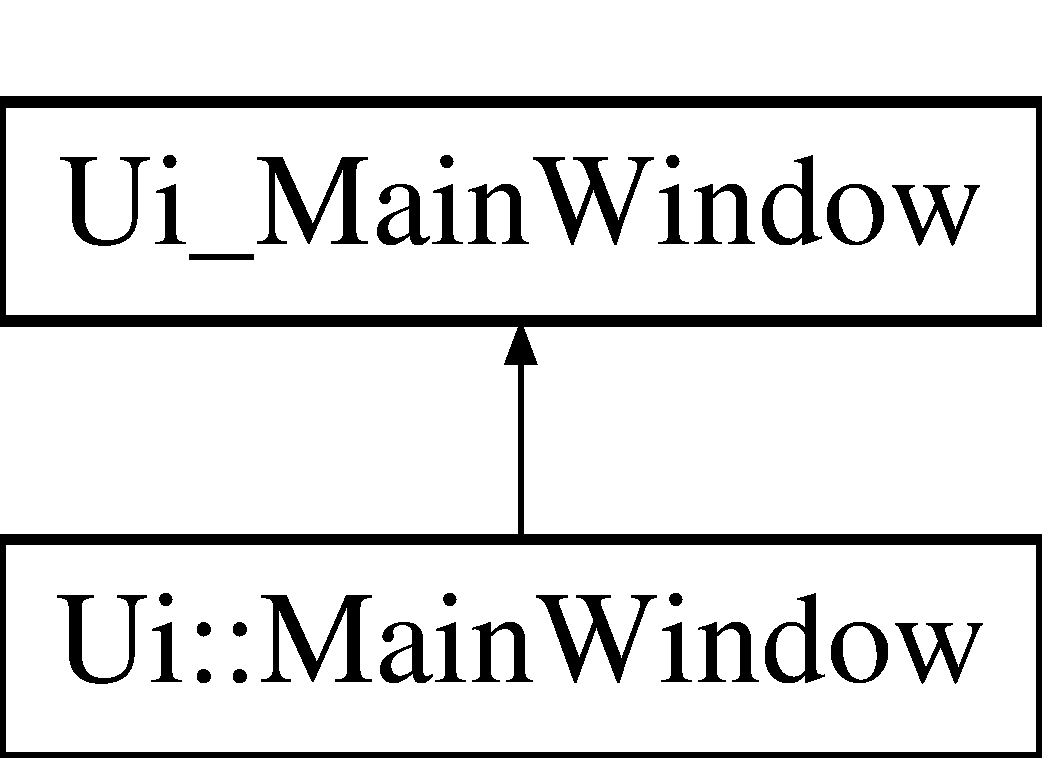
\includegraphics[height=2.000000cm]{class_ui_1_1_main_window}
\end{center}
\end{figure}
\subsection*{Additional Inherited Members}


\subsection{Detailed Description}


Definition at line 91 of file ui\-\_\-mainwindow.\-h.



The documentation for this class was generated from the following file\-:\begin{DoxyCompactItemize}
\item 
Scrabble/\hyperlink{ui__mainwindow_8h}{ui\-\_\-mainwindow.\-h}\end{DoxyCompactItemize}

\hypertarget{class_move}{\section{Move Class Reference}
\label{class_move}\index{Move@{Move}}
}


The \hyperlink{class_move}{Move} class Contains a single move from a \hyperlink{class_rack}{Rack} to the \hyperlink{class_board}{Board}.  




{\ttfamily \#include $<$move.\-h$>$}

\subsection*{Public Member Functions}
\begin{DoxyCompactItemize}
\item 
\hyperlink{class_move_a6bf1a65d4c0e23849cedfb56ed27046a}{Move} (\hyperlink{class_player}{Player} $\ast$, \hyperlink{class_letter}{Letter} $\ast$, int, int, int)
\begin{DoxyCompactList}\small\item\em \hyperlink{class_move_a6bf1a65d4c0e23849cedfb56ed27046a}{Move\-::\-Move} Constructor. \end{DoxyCompactList}\item 
\hyperlink{class_player}{Player} $\ast$ \hyperlink{class_move_a4b3a579f0516de5a8eda9cc6dfe88eab}{get\-Player} ()
\begin{DoxyCompactList}\small\item\em \hyperlink{class_move_a4b3a579f0516de5a8eda9cc6dfe88eab}{Move\-::get\-Player} Getter for player. \end{DoxyCompactList}\item 
\hyperlink{class_letter}{Letter} $\ast$ \hyperlink{class_move_a0c29654c98269d65c6af694eb441d382}{get\-Letter} ()
\begin{DoxyCompactList}\small\item\em \hyperlink{class_move_a0c29654c98269d65c6af694eb441d382}{Move\-::get\-Letter} Getter for \hyperlink{class_letter}{Letter}. \end{DoxyCompactList}\item 
int \hyperlink{class_move_a7e3169f48fcca1aa1de4a5cbe67a284d}{get\-X} ()
\begin{DoxyCompactList}\small\item\em \hyperlink{class_move_a7e3169f48fcca1aa1de4a5cbe67a284d}{Move\-::get\-X} Getter for board\-X. \end{DoxyCompactList}\item 
int \hyperlink{class_move_af388d15d91f61a1f909998f50988ac1a}{get\-Y} ()
\begin{DoxyCompactList}\small\item\em \hyperlink{class_move_af388d15d91f61a1f909998f50988ac1a}{Move\-::get\-Y} Getter for bord\-Y. \end{DoxyCompactList}\item 
int \hyperlink{class_move_ad78bb76d9b590cdb98aa4d4a3088e69d}{get\-Rack\-Position} ()
\begin{DoxyCompactList}\small\item\em \hyperlink{class_move_ad78bb76d9b590cdb98aa4d4a3088e69d}{Move\-::get\-Rack\-Position} Gets the position this letter draws from, from the rack. \end{DoxyCompactList}\item 
\hyperlink{class_move}{Move} $\ast$ \hyperlink{class_move_af3c01fad2f5724f497a2d9eb165be470}{apply} ()
\begin{DoxyCompactList}\small\item\em \hyperlink{class_move_af3c01fad2f5724f497a2d9eb165be470}{Move\-::apply} Applies to the board. \end{DoxyCompactList}\item 
\hyperlink{class_move}{Move} $\ast$ \hyperlink{class_move_a2ca5c1f8be73c0e6c0ec4b359061a1e2}{unapply} ()
\begin{DoxyCompactList}\small\item\em \hyperlink{class_move_a2ca5c1f8be73c0e6c0ec4b359061a1e2}{Move\-::unapply} Unapplies from the board. \end{DoxyCompactList}\item 
\hyperlink{class_move}{Move} $\ast$ \hyperlink{class_move_a315c3ce190a5a9ef24cf6cc5916e81b1}{finalize} ()
\begin{DoxyCompactList}\small\item\em \hyperlink{class_move_a315c3ce190a5a9ef24cf6cc5916e81b1}{Move\-::finalize} Finalizes the board. \end{DoxyCompactList}\end{DoxyCompactItemize}
\subsection*{Private Attributes}
\begin{DoxyCompactItemize}
\item 
\hyperlink{class_player}{Player} $\ast$ \hyperlink{class_move_a1fbc388e091cd5639b755ebca2a8f90b}{player}
\item 
\hyperlink{class_letter}{Letter} $\ast$ \hyperlink{class_move_a80fe73cecfae0270265a8d5a50a9739f}{letter}
\item 
int \hyperlink{class_move_a8a1c46caedcac551e4a6714b7b729a41}{rack\-Position}
\item 
int \hyperlink{class_move_ad3fa58a6db17896f2a83cbcc77ceb998}{board\-X}
\item 
int \hyperlink{class_move_ac953ac3b9b8ca529d1be967c7712ae05}{board\-Y}
\end{DoxyCompactItemize}


\subsection{Detailed Description}
The \hyperlink{class_move}{Move} class Contains a single move from a \hyperlink{class_rack}{Rack} to the \hyperlink{class_board}{Board}. 

Definition at line 12 of file move.\-h.



\subsection{Constructor \& Destructor Documentation}
\hypertarget{class_move_a6bf1a65d4c0e23849cedfb56ed27046a}{\index{Move@{Move}!Move@{Move}}
\index{Move@{Move}!Move@{Move}}
\subsubsection[{Move}]{\setlength{\rightskip}{0pt plus 5cm}Move\-::\-Move (
\begin{DoxyParamCaption}
\item[{{\bf Player} $\ast$}]{player, }
\item[{{\bf Letter} $\ast$}]{letter, }
\item[{int}]{rack\-Position, }
\item[{int}]{board\-X, }
\item[{int}]{board\-Y}
\end{DoxyParamCaption}
)}}\label{class_move_a6bf1a65d4c0e23849cedfb56ed27046a}


\hyperlink{class_move_a6bf1a65d4c0e23849cedfb56ed27046a}{Move\-::\-Move} Constructor. 


\begin{DoxyParams}{Parameters}
{\em player} & The player \\
\hline
{\em letter} & The letter \\
\hline
{\em rack\-Position} & The position in the rack \\
\hline
{\em board\-X} & The x position on the board \\
\hline
{\em board\-Y} & The y position on the board \\
\hline
\end{DoxyParams}


Definition at line 11 of file move.\-cpp.



References board\-X, board\-Y, letter, player, and rack\-Position.


\begin{DoxyCode}
11                                                                                   \{
12     this->player = \hyperlink{class_move_a1fbc388e091cd5639b755ebca2a8f90b}{player};
13     this->letter = \hyperlink{class_move_a80fe73cecfae0270265a8d5a50a9739f}{letter};
14     this->\hyperlink{class_move_a8a1c46caedcac551e4a6714b7b729a41}{rackPosition} = \hyperlink{class_move_a8a1c46caedcac551e4a6714b7b729a41}{rackPosition};
15     this->\hyperlink{class_move_ad3fa58a6db17896f2a83cbcc77ceb998}{boardX} = \hyperlink{class_move_ad3fa58a6db17896f2a83cbcc77ceb998}{boardX};
16     this->\hyperlink{class_move_ac953ac3b9b8ca529d1be967c7712ae05}{boardY} = \hyperlink{class_move_ac953ac3b9b8ca529d1be967c7712ae05}{boardY};
17 \}
\end{DoxyCode}


\subsection{Member Function Documentation}
\hypertarget{class_move_af3c01fad2f5724f497a2d9eb165be470}{\index{Move@{Move}!apply@{apply}}
\index{apply@{apply}!Move@{Move}}
\subsubsection[{apply}]{\setlength{\rightskip}{0pt plus 5cm}{\bf Move} $\ast$ Move\-::apply (
\begin{DoxyParamCaption}
{}
\end{DoxyParamCaption}
)}}\label{class_move_af3c01fad2f5724f497a2d9eb165be470}


\hyperlink{class_move_af3c01fad2f5724f497a2d9eb165be470}{Move\-::apply} Applies to the board. 

\begin{DoxyReturn}{Returns}
this 
\end{DoxyReturn}


Definition at line 68 of file move.\-cpp.



References board\-X, board\-Y, Board\-::get\-Board(), Space\-::get\-Letter(), Rack\-::get\-Rack(), Rack\-::get\-Space(), Space\-::is\-Inactive(), rack\-Position, Space\-::set\-Letter(), Space\-::set\-New(), Space\-::set\-Placed(), and Board\-::spaces.



Referenced by Board\-::move\-Letter\-To\-Board().


\begin{DoxyCode}
69 \{
70     \hyperlink{class_space}{Space} *boardSpace = \hyperlink{class_board_ae30e802b1d83309fc95e695b5b3df338}{Board::getBoard}()->\hyperlink{class_board_a73b12248ddb6ee3adc24f4458d8661c2}{spaces}[
      \hyperlink{class_move_ad3fa58a6db17896f2a83cbcc77ceb998}{boardX}][\hyperlink{class_move_ac953ac3b9b8ca529d1be967c7712ae05}{boardY}];
71     \textcolor{keywordflow}{if}(boardSpace->\hyperlink{class_space_a83819948ab0508299c66829ca8335034}{isInactive}())\{
72         \hyperlink{class_space}{Space} *rackSpace = \hyperlink{class_rack_aa48de650c15bda8267451d84caf6ea3f}{Rack::getRack}()->\hyperlink{class_rack_a2fdfa2264bb85c08ebf107e67cfc8657}{getSpace}(
      \hyperlink{class_move_a8a1c46caedcac551e4a6714b7b729a41}{rackPosition});
73         boardSpace->\hyperlink{class_space_aab86690461768d190a009e06c753f2ce}{setLetter}(rackSpace->\hyperlink{class_space_a207bc025538775ce43bdcc0d8c4c3599}{getLetter}());
74         rackSpace->\hyperlink{class_space_a092351d8c32b8f89a78fc475a49b3b21}{setPlaced}();
75         boardSpace->\hyperlink{class_space_a3afac453f54e569a94164c41a9721643}{setNew}();
76     \}
77     \textcolor{keywordflow}{return} \textcolor{keyword}{this};
78 \}
\end{DoxyCode}
\hypertarget{class_move_a315c3ce190a5a9ef24cf6cc5916e81b1}{\index{Move@{Move}!finalize@{finalize}}
\index{finalize@{finalize}!Move@{Move}}
\subsubsection[{finalize}]{\setlength{\rightskip}{0pt plus 5cm}{\bf Move} $\ast$ Move\-::finalize (
\begin{DoxyParamCaption}
{}
\end{DoxyParamCaption}
)}}\label{class_move_a315c3ce190a5a9ef24cf6cc5916e81b1}


\hyperlink{class_move_a315c3ce190a5a9ef24cf6cc5916e81b1}{Move\-::finalize} Finalizes the board. 

\begin{DoxyReturn}{Returns}
this 
\end{DoxyReturn}


Definition at line 100 of file move.\-cpp.



References board\-X, board\-Y, Board\-::get\-Board(), Space\-::set\-On\-Board(), and Board\-::spaces.


\begin{DoxyCode}
101 \{
102     \hyperlink{class_board_ae30e802b1d83309fc95e695b5b3df338}{Board::getBoard}()->\hyperlink{class_board_a73b12248ddb6ee3adc24f4458d8661c2}{spaces}[\hyperlink{class_move_ad3fa58a6db17896f2a83cbcc77ceb998}{boardX}][\hyperlink{class_move_ac953ac3b9b8ca529d1be967c7712ae05}{boardY}]->
      \hyperlink{class_space_ae565aeac581e7ac3ab35b1f900140e3f}{setOnBoard}();
103 
104     \textcolor{keywordflow}{return} \textcolor{keyword}{this};
105 \}
\end{DoxyCode}
\hypertarget{class_move_a0c29654c98269d65c6af694eb441d382}{\index{Move@{Move}!get\-Letter@{get\-Letter}}
\index{get\-Letter@{get\-Letter}!Move@{Move}}
\subsubsection[{get\-Letter}]{\setlength{\rightskip}{0pt plus 5cm}{\bf Letter} $\ast$ Move\-::get\-Letter (
\begin{DoxyParamCaption}
{}
\end{DoxyParamCaption}
)}}\label{class_move_a0c29654c98269d65c6af694eb441d382}


\hyperlink{class_move_a0c29654c98269d65c6af694eb441d382}{Move\-::get\-Letter} Getter for \hyperlink{class_letter}{Letter}. 

\begin{DoxyReturn}{Returns}
letter 
\end{DoxyReturn}


Definition at line 59 of file move.\-cpp.



References letter.



Referenced by Play\-::clear\-Letter(), Play\-::get\-Char\-Array(), and A\-I\-Player\-::play().


\begin{DoxyCode}
60 \{
61     \textcolor{keywordflow}{return} \hyperlink{class_move_a80fe73cecfae0270265a8d5a50a9739f}{letter};
62 \}
\end{DoxyCode}
\hypertarget{class_move_a4b3a579f0516de5a8eda9cc6dfe88eab}{\index{Move@{Move}!get\-Player@{get\-Player}}
\index{get\-Player@{get\-Player}!Move@{Move}}
\subsubsection[{get\-Player}]{\setlength{\rightskip}{0pt plus 5cm}{\bf Player} $\ast$ Move\-::get\-Player (
\begin{DoxyParamCaption}
{}
\end{DoxyParamCaption}
)}}\label{class_move_a4b3a579f0516de5a8eda9cc6dfe88eab}


\hyperlink{class_move_a4b3a579f0516de5a8eda9cc6dfe88eab}{Move\-::get\-Player} Getter for player. 

\begin{DoxyReturn}{Returns}
player 
\end{DoxyReturn}


Definition at line 50 of file move.\-cpp.



References player.


\begin{DoxyCode}
51 \{
52     \textcolor{keywordflow}{return} \hyperlink{class_move_a1fbc388e091cd5639b755ebca2a8f90b}{player};
53 \}
\end{DoxyCode}
\hypertarget{class_move_ad78bb76d9b590cdb98aa4d4a3088e69d}{\index{Move@{Move}!get\-Rack\-Position@{get\-Rack\-Position}}
\index{get\-Rack\-Position@{get\-Rack\-Position}!Move@{Move}}
\subsubsection[{get\-Rack\-Position}]{\setlength{\rightskip}{0pt plus 5cm}int Move\-::get\-Rack\-Position (
\begin{DoxyParamCaption}
{}
\end{DoxyParamCaption}
)}}\label{class_move_ad78bb76d9b590cdb98aa4d4a3088e69d}


\hyperlink{class_move_ad78bb76d9b590cdb98aa4d4a3088e69d}{Move\-::get\-Rack\-Position} Gets the position this letter draws from, from the rack. 

\begin{DoxyReturn}{Returns}
rackposition. 
\end{DoxyReturn}


Definition at line 41 of file move.\-cpp.



References rack\-Position.



Referenced by A\-I\-Player\-::play().


\begin{DoxyCode}
42 \{
43     \textcolor{keywordflow}{return} \hyperlink{class_move_a8a1c46caedcac551e4a6714b7b729a41}{rackPosition};
44 \}
\end{DoxyCode}
\hypertarget{class_move_a7e3169f48fcca1aa1de4a5cbe67a284d}{\index{Move@{Move}!get\-X@{get\-X}}
\index{get\-X@{get\-X}!Move@{Move}}
\subsubsection[{get\-X}]{\setlength{\rightskip}{0pt plus 5cm}int Move\-::get\-X (
\begin{DoxyParamCaption}
{}
\end{DoxyParamCaption}
)}}\label{class_move_a7e3169f48fcca1aa1de4a5cbe67a284d}


\hyperlink{class_move_a7e3169f48fcca1aa1de4a5cbe67a284d}{Move\-::get\-X} Getter for board\-X. 

\begin{DoxyReturn}{Returns}
board\-X 
\end{DoxyReturn}


Definition at line 23 of file move.\-cpp.



References board\-X.



Referenced by A\-I\-Player\-::play(), and Play\-::validate().


\begin{DoxyCode}
24 \{
25     \textcolor{keywordflow}{return} \hyperlink{class_move_ad3fa58a6db17896f2a83cbcc77ceb998}{boardX};
26 \}
\end{DoxyCode}
\hypertarget{class_move_af388d15d91f61a1f909998f50988ac1a}{\index{Move@{Move}!get\-Y@{get\-Y}}
\index{get\-Y@{get\-Y}!Move@{Move}}
\subsubsection[{get\-Y}]{\setlength{\rightskip}{0pt plus 5cm}int Move\-::get\-Y (
\begin{DoxyParamCaption}
{}
\end{DoxyParamCaption}
)}}\label{class_move_af388d15d91f61a1f909998f50988ac1a}


\hyperlink{class_move_af388d15d91f61a1f909998f50988ac1a}{Move\-::get\-Y} Getter for bord\-Y. 

\begin{DoxyReturn}{Returns}
board\-Y 
\end{DoxyReturn}


Definition at line 32 of file move.\-cpp.



References board\-Y.



Referenced by A\-I\-Player\-::play(), and Play\-::validate().


\begin{DoxyCode}
33 \{
34     \textcolor{keywordflow}{return} \hyperlink{class_move_ac953ac3b9b8ca529d1be967c7712ae05}{boardY};
35 \}
\end{DoxyCode}
\hypertarget{class_move_a2ca5c1f8be73c0e6c0ec4b359061a1e2}{\index{Move@{Move}!unapply@{unapply}}
\index{unapply@{unapply}!Move@{Move}}
\subsubsection[{unapply}]{\setlength{\rightskip}{0pt plus 5cm}{\bf Move} $\ast$ Move\-::unapply (
\begin{DoxyParamCaption}
{}
\end{DoxyParamCaption}
)}}\label{class_move_a2ca5c1f8be73c0e6c0ec4b359061a1e2}


\hyperlink{class_move_a2ca5c1f8be73c0e6c0ec4b359061a1e2}{Move\-::unapply} Unapplies from the board. 

\begin{DoxyReturn}{Returns}
this 
\end{DoxyReturn}


Definition at line 84 of file move.\-cpp.



References board\-X, board\-Y, Board\-::get\-Board(), Rack\-::get\-Rack(), Rack\-::get\-Space(), Space\-::is\-Inactive(), rack\-Position, Space\-::set\-Inactive(), Space\-::set\-Letter(), and Board\-::spaces.


\begin{DoxyCode}
85 \{
86     \hyperlink{class_space}{Space} *boardSpace = \hyperlink{class_board_ae30e802b1d83309fc95e695b5b3df338}{Board::getBoard}()->\hyperlink{class_board_a73b12248ddb6ee3adc24f4458d8661c2}{spaces}[
      \hyperlink{class_move_ad3fa58a6db17896f2a83cbcc77ceb998}{boardX}][\hyperlink{class_move_ac953ac3b9b8ca529d1be967c7712ae05}{boardY}];
87     \textcolor{keywordflow}{if}(!boardSpace->\hyperlink{class_space_a83819948ab0508299c66829ca8335034}{isInactive}())\{
88         \hyperlink{class_space}{Space} *rackSpace = \hyperlink{class_rack_aa48de650c15bda8267451d84caf6ea3f}{Rack::getRack}()->\hyperlink{class_rack_a2fdfa2264bb85c08ebf107e67cfc8657}{getSpace}(
      \hyperlink{class_move_a8a1c46caedcac551e4a6714b7b729a41}{rackPosition});
89         boardSpace->\hyperlink{class_space_aab86690461768d190a009e06c753f2ce}{setLetter}(NULL);
90         rackSpace->\hyperlink{class_space_a8f6b89f570c1e0ca3c34f19df439a598}{setInactive}();
91         boardSpace->\hyperlink{class_space_a8f6b89f570c1e0ca3c34f19df439a598}{setInactive}();
92     \}
93     \textcolor{keywordflow}{return} \textcolor{keyword}{this};
94 \}
\end{DoxyCode}


\subsection{Member Data Documentation}
\hypertarget{class_move_ad3fa58a6db17896f2a83cbcc77ceb998}{\index{Move@{Move}!board\-X@{board\-X}}
\index{board\-X@{board\-X}!Move@{Move}}
\subsubsection[{board\-X}]{\setlength{\rightskip}{0pt plus 5cm}int Move\-::board\-X\hspace{0.3cm}{\ttfamily [private]}}}\label{class_move_ad3fa58a6db17896f2a83cbcc77ceb998}
The x position on the board 

Definition at line 31 of file move.\-h.



Referenced by apply(), finalize(), get\-X(), Move(), and unapply().

\hypertarget{class_move_ac953ac3b9b8ca529d1be967c7712ae05}{\index{Move@{Move}!board\-Y@{board\-Y}}
\index{board\-Y@{board\-Y}!Move@{Move}}
\subsubsection[{board\-Y}]{\setlength{\rightskip}{0pt plus 5cm}int Move\-::board\-Y\hspace{0.3cm}{\ttfamily [private]}}}\label{class_move_ac953ac3b9b8ca529d1be967c7712ae05}
The y position on the board 

Definition at line 32 of file move.\-h.



Referenced by apply(), finalize(), get\-Y(), Move(), and unapply().

\hypertarget{class_move_a80fe73cecfae0270265a8d5a50a9739f}{\index{Move@{Move}!letter@{letter}}
\index{letter@{letter}!Move@{Move}}
\subsubsection[{letter}]{\setlength{\rightskip}{0pt plus 5cm}{\bf Letter}$\ast$ Move\-::letter\hspace{0.3cm}{\ttfamily [private]}}}\label{class_move_a80fe73cecfae0270265a8d5a50a9739f}
The \hyperlink{class_letter}{Letter} 

Definition at line 29 of file move.\-h.



Referenced by get\-Letter(), and Move().

\hypertarget{class_move_a1fbc388e091cd5639b755ebca2a8f90b}{\index{Move@{Move}!player@{player}}
\index{player@{player}!Move@{Move}}
\subsubsection[{player}]{\setlength{\rightskip}{0pt plus 5cm}{\bf Player}$\ast$ Move\-::player\hspace{0.3cm}{\ttfamily [private]}}}\label{class_move_a1fbc388e091cd5639b755ebca2a8f90b}
The \hyperlink{class_player}{Player} who made the move 

Definition at line 28 of file move.\-h.



Referenced by get\-Player(), and Move().

\hypertarget{class_move_a8a1c46caedcac551e4a6714b7b729a41}{\index{Move@{Move}!rack\-Position@{rack\-Position}}
\index{rack\-Position@{rack\-Position}!Move@{Move}}
\subsubsection[{rack\-Position}]{\setlength{\rightskip}{0pt plus 5cm}int Move\-::rack\-Position\hspace{0.3cm}{\ttfamily [private]}}}\label{class_move_a8a1c46caedcac551e4a6714b7b729a41}
The position on the rack it came from 

Definition at line 30 of file move.\-h.



Referenced by apply(), get\-Rack\-Position(), Move(), and unapply().



The documentation for this class was generated from the following files\-:\begin{DoxyCompactItemize}
\item 
Scrabble/\hyperlink{move_8h}{move.\-h}\item 
Scrabble/\hyperlink{move_8cpp}{move.\-cpp}\end{DoxyCompactItemize}

\hypertarget{class_play}{\section{Play Class Reference}
\label{class_play}\index{Play@{Play}}
}


The \hyperlink{class_play}{Play} class Wrapper for a set of Moves that make up a \hyperlink{class_play}{Play}.  




{\ttfamily \#include $<$play.\-h$>$}

\subsection*{Public Member Functions}
\begin{DoxyCompactItemize}
\item 
\hyperlink{class_play_a2dc24501b99a45769193fcb270505f0f}{Play} (Q\-List$<$ \hyperlink{class_move}{Move} $\ast$ $>$ $\ast$, \hyperlink{class_player}{Player} $\ast$)
\begin{DoxyCompactList}\small\item\em \hyperlink{class_play_a2dc24501b99a45769193fcb270505f0f}{Play\-::\-Play} Constructor. \end{DoxyCompactList}\item 
\hyperlink{class_play_a0088438837d29378e35a2beed04e64df}{Play} ()
\begin{DoxyCompactList}\small\item\em \hyperlink{class_play}{Play} class constructor. \end{DoxyCompactList}\item 
\hyperlink{class_play_aa0a6845d214673a3dc64d661027046b2}{Play} (const \hyperlink{class_play}{Play} \&other)
\begin{DoxyCompactList}\small\item\em \hyperlink{class_play_a2dc24501b99a45769193fcb270505f0f}{Play\-::\-Play} Copy Constructor. \end{DoxyCompactList}\item 
\hyperlink{class_play_a6f7dd4d097454caef2e81fa94fe739d5}{$\sim$\-Play} ()
\begin{DoxyCompactList}\small\item\em \hyperlink{class_play}{Play} destructor. \end{DoxyCompactList}\item 
bool \hyperlink{class_play_af3ee40c18a0e3fbf6e16f645b8de248b}{is\-Empty} ()
\begin{DoxyCompactList}\small\item\em \hyperlink{class_play_af3ee40c18a0e3fbf6e16f645b8de248b}{Play\-::is\-Empty}, checks whether the move vector has any elements. \end{DoxyCompactList}\item 
bool \hyperlink{class_play_a498e6c1b124296872e22151e8ee965fb}{validate} (\hyperlink{class_dictionary}{Dictionary} \&dict)
\begin{DoxyCompactList}\small\item\em \hyperlink{class_play_a498e6c1b124296872e22151e8ee965fb}{Play\-::validate} will return whether or not this is a valid play on the board. \end{DoxyCompactList}\item 
\hyperlink{class_play}{Play} $\ast$ \hyperlink{class_play_ad70d9b77395e7b30506d1c38ace45bf0}{add\-Move} (\hyperlink{class_player}{Player} $\ast$, \hyperlink{class_move}{Move} $\ast$)
\begin{DoxyCompactList}\small\item\em \hyperlink{class_play_ad70d9b77395e7b30506d1c38ace45bf0}{Play\-::add\-Move}, adds a single move to the list of plays. \end{DoxyCompactList}\item 
\hyperlink{class_play}{Play} $\ast$ \hyperlink{class_play_a5b6d4e2fafc15310485d4770ae36e46e}{apply\-Moves} ()
\begin{DoxyCompactList}\small\item\em \hyperlink{class_play_a5b6d4e2fafc15310485d4770ae36e46e}{Play\-::apply\-Moves} temporarily applies each move of the play to the board. \end{DoxyCompactList}\item 
\hyperlink{class_play}{Play} $\ast$ \hyperlink{class_play_a56788c5adf1bdc5230bf226f6a97dd04}{unapply\-Moves} ()
\begin{DoxyCompactList}\small\item\em \hyperlink{class_play_a56788c5adf1bdc5230bf226f6a97dd04}{Play\-::unapply\-Moves} does the opposite of the temporary placement, and inactivates the spaces. \end{DoxyCompactList}\item 
\hyperlink{class_play}{Play} $\ast$ \hyperlink{class_play_a02fbcafed804466c41fd78e8eef8ca16}{finalize\-Moves} ()
\begin{DoxyCompactList}\small\item\em \hyperlink{class_play_a02fbcafed804466c41fd78e8eef8ca16}{Play\-::finalize\-Moves} Permanently adds each move of the play to the board. \end{DoxyCompactList}\item 
\hyperlink{class_play}{Play} $\ast$ \hyperlink{class_play_af9f4b1daff13026dd4f38f93375f576f}{clear\-Moves} ()
\begin{DoxyCompactList}\small\item\em \hyperlink{class_play_af9f4b1daff13026dd4f38f93375f576f}{Play\-::clear\-Moves} removes all elements from the play list. \end{DoxyCompactList}\item 
\hyperlink{class_play}{Play} $\ast$ \hyperlink{class_play_a034c9cc986629045cdfcdbdeaabb2ab4}{clear\-Letter} (\hyperlink{class_letter}{Letter} $\ast$)
\begin{DoxyCompactList}\small\item\em \hyperlink{class_play_a034c9cc986629045cdfcdbdeaabb2ab4}{Play\-::clear\-Letter} Clears a move by the Letter$\ast$ it contains. \end{DoxyCompactList}\item 
int \hyperlink{class_play_a2311eaa432738b08a75d7ca35af46ba6}{size} ()
\begin{DoxyCompactList}\small\item\em \hyperlink{class_play_a2311eaa432738b08a75d7ca35af46ba6}{Play\-::size}, checks the number of moves in a play. \end{DoxyCompactList}\item 
class \hyperlink{class_player}{Player} $\ast$ \hyperlink{class_play_aebe81c706ee1005b63fad43f2eaff0c0}{get\-Player} ()
\begin{DoxyCompactList}\small\item\em \hyperlink{class_play_aebe81c706ee1005b63fad43f2eaff0c0}{Play\-::get\-Player}. \end{DoxyCompactList}\item 
int \hyperlink{class_play_af2599835f6eba8136770a4f773a9f9ef}{get\-Value} ()
\begin{DoxyCompactList}\small\item\em \hyperlink{class_play_af2599835f6eba8136770a4f773a9f9ef}{Play\-::get\-Value}, checks the value of the current play. \end{DoxyCompactList}\item 
Q\-String \hyperlink{class_play_a609ee8aa7d127a27ace83fa47b1478a9}{get\-Char\-Array} ()
\begin{DoxyCompactList}\small\item\em \hyperlink{class_play_a609ee8aa7d127a27ace83fa47b1478a9}{Play\-::get\-Char\-Array} gets the \hyperlink{class_play}{Play}'s moves in the form of a string. \end{DoxyCompactList}\end{DoxyCompactItemize}
\subsection*{Private Member Functions}
\begin{DoxyCompactItemize}
\item 
bool \hyperlink{class_play_a6699a989cb202ffc8db61093fea15d1f}{validate\-\_\-right} (int x\-\_\-start, int y, \hyperlink{class_dictionary}{Dictionary} \&dict, \hyperlink{class_board}{Board} $\ast$myboard)
\begin{DoxyCompactList}\small\item\em \hyperlink{class_play_a6699a989cb202ffc8db61093fea15d1f}{Play\-::validate\-\_\-right} Validates a \hyperlink{class_play}{Play} to the right. \end{DoxyCompactList}\item 
bool \hyperlink{class_play_ae7096a77ed85b5251f2faccfb092616b}{validate\-\_\-down} (int y\-\_\-start, int x, \hyperlink{class_dictionary}{Dictionary} \&dict, \hyperlink{class_board}{Board} $\ast$myboard)
\begin{DoxyCompactList}\small\item\em \hyperlink{class_play_ae7096a77ed85b5251f2faccfb092616b}{Play\-::validate\-\_\-down} Validates a \hyperlink{class_play}{Play} downward. \end{DoxyCompactList}\end{DoxyCompactItemize}
\subsection*{Private Attributes}
\begin{DoxyCompactItemize}
\item 
Q\-List$<$ \hyperlink{class_move}{Move} $\ast$ $>$ $\ast$ \hyperlink{class_play_ade35ae53bff24e1755a935899ee018ed}{moves}
\item 
\hyperlink{class_player}{Player} $\ast$ \hyperlink{class_play_a8a7094a8a0186212896fe7daf71617a3}{player}
\item 
int \hyperlink{class_play_abc8cb0f8fb660091fee8563b5a917ad7}{value}
\end{DoxyCompactItemize}
\subsection*{Friends}
\begin{DoxyCompactItemize}
\item 
class \hyperlink{class_play_a2c11a076a909acd936d897cd2a81f931}{A\-I\-Player}
\end{DoxyCompactItemize}


\subsection{Detailed Description}
The \hyperlink{class_play}{Play} class Wrapper for a set of Moves that make up a \hyperlink{class_play}{Play}. 

Definition at line 16 of file play.\-h.



\subsection{Constructor \& Destructor Documentation}
\hypertarget{class_play_a2dc24501b99a45769193fcb270505f0f}{\index{Play@{Play}!Play@{Play}}
\index{Play@{Play}!Play@{Play}}
\subsubsection[{Play}]{\setlength{\rightskip}{0pt plus 5cm}Play\-::\-Play (
\begin{DoxyParamCaption}
\item[{Q\-List$<$ {\bf Move} $\ast$ $>$ $\ast$}]{moves, }
\item[{{\bf Player} $\ast$}]{player}
\end{DoxyParamCaption}
)}}\label{class_play_a2dc24501b99a45769193fcb270505f0f}


\hyperlink{class_play_a2dc24501b99a45769193fcb270505f0f}{Play\-::\-Play} Constructor. 


\begin{DoxyParams}{Parameters}
{\em moves} & A list of moves \\
\hline
{\em player} & The player \\
\hline
\end{DoxyParams}


Definition at line 18 of file play.\-cpp.



References player, and value.


\begin{DoxyCode}
19 \{
20     this->\hyperlink{class_play_ade35ae53bff24e1755a935899ee018ed}{moves} = \textcolor{keyword}{new} QList<Move*>();
21     this->\hyperlink{class_play_abc8cb0f8fb660091fee8563b5a917ad7}{value} = 0;
22     \textcolor{keywordflow}{for}(\textcolor{keywordtype}{int} i = 0; i < \hyperlink{class_play_ade35ae53bff24e1755a935899ee018ed}{moves}->size(); i++) \{
23         this->\hyperlink{class_play_ade35ae53bff24e1755a935899ee018ed}{moves}->insert(i,\textcolor{keyword}{new} \hyperlink{class_move}{Move}(*\hyperlink{class_play_ade35ae53bff24e1755a935899ee018ed}{moves}->at(i)));
24         this->value += this->\hyperlink{class_play_ade35ae53bff24e1755a935899ee018ed}{moves}->at(i)->getLetter()->getValue();
25     \}
26     \textcolor{comment}{// this->moves = moves;}
27     this->player = \hyperlink{class_play_a8a7094a8a0186212896fe7daf71617a3}{player};
28 \}
\end{DoxyCode}
\hypertarget{class_play_a0088438837d29378e35a2beed04e64df}{\index{Play@{Play}!Play@{Play}}
\index{Play@{Play}!Play@{Play}}
\subsubsection[{Play}]{\setlength{\rightskip}{0pt plus 5cm}Play\-::\-Play (
\begin{DoxyParamCaption}
{}
\end{DoxyParamCaption}
)}}\label{class_play_a0088438837d29378e35a2beed04e64df}


\hyperlink{class_play}{Play} class constructor. 



Definition at line 6 of file play.\-cpp.



References moves, player, and value.


\begin{DoxyCode}
7 \{
8     this->\hyperlink{class_play_ade35ae53bff24e1755a935899ee018ed}{moves} = \textcolor{keyword}{new} QList<Move*>();
9     this->\hyperlink{class_play_abc8cb0f8fb660091fee8563b5a917ad7}{value} = 0;
10     this->\hyperlink{class_play_a8a7094a8a0186212896fe7daf71617a3}{player} = 0;
11 \}
\end{DoxyCode}
\hypertarget{class_play_aa0a6845d214673a3dc64d661027046b2}{\index{Play@{Play}!Play@{Play}}
\index{Play@{Play}!Play@{Play}}
\subsubsection[{Play}]{\setlength{\rightskip}{0pt plus 5cm}Play\-::\-Play (
\begin{DoxyParamCaption}
\item[{const {\bf Play} \&}]{other}
\end{DoxyParamCaption}
)}}\label{class_play_aa0a6845d214673a3dc64d661027046b2}


\hyperlink{class_play_a2dc24501b99a45769193fcb270505f0f}{Play\-::\-Play} Copy Constructor. 


\begin{DoxyParams}{Parameters}
{\em other} & Other \hyperlink{class_play}{Play} \\
\hline
\end{DoxyParams}


Definition at line 239 of file play.\-cpp.



References moves, player, and value.


\begin{DoxyCode}
239                             \{
240     this->\hyperlink{class_play_a8a7094a8a0186212896fe7daf71617a3}{player} = other.\hyperlink{class_play_a8a7094a8a0186212896fe7daf71617a3}{player};
241     this->\hyperlink{class_play_abc8cb0f8fb660091fee8563b5a917ad7}{value} = other.\hyperlink{class_play_abc8cb0f8fb660091fee8563b5a917ad7}{value};
242     this->\hyperlink{class_play_ade35ae53bff24e1755a935899ee018ed}{moves} = \textcolor{keyword}{new} QList<Move*>();
243     \textcolor{keywordtype}{int} i = 0;
244     \textcolor{keywordflow}{for}(QList<Move*>::ConstIterator it = other.\hyperlink{class_play_ade35ae53bff24e1755a935899ee018ed}{moves}->cbegin(); it != other.
      \hyperlink{class_play_ade35ae53bff24e1755a935899ee018ed}{moves}->cend(); it++)
245     \{
246         \hyperlink{class_move}{Move} * curmove = *it;
247         this->\hyperlink{class_play_ade35ae53bff24e1755a935899ee018ed}{moves}->insert(i,curmove);
248         i++;
249     \}
250 \}
\end{DoxyCode}
\hypertarget{class_play_a6f7dd4d097454caef2e81fa94fe739d5}{\index{Play@{Play}!$\sim$\-Play@{$\sim$\-Play}}
\index{$\sim$\-Play@{$\sim$\-Play}!Play@{Play}}
\subsubsection[{$\sim$\-Play}]{\setlength{\rightskip}{0pt plus 5cm}Play\-::$\sim$\-Play (
\begin{DoxyParamCaption}
{}
\end{DoxyParamCaption}
)}}\label{class_play_a6f7dd4d097454caef2e81fa94fe739d5}


\hyperlink{class_play}{Play} destructor. 



Definition at line 33 of file play.\-cpp.



References clear\-Moves().


\begin{DoxyCode}
34 \{
35     \hyperlink{class_play_af9f4b1daff13026dd4f38f93375f576f}{clearMoves}();
36 \}
\end{DoxyCode}


\subsection{Member Function Documentation}
\hypertarget{class_play_ad70d9b77395e7b30506d1c38ace45bf0}{\index{Play@{Play}!add\-Move@{add\-Move}}
\index{add\-Move@{add\-Move}!Play@{Play}}
\subsubsection[{add\-Move}]{\setlength{\rightskip}{0pt plus 5cm}{\bf Play} $\ast$ Play\-::add\-Move (
\begin{DoxyParamCaption}
\item[{{\bf Player} $\ast$}]{player, }
\item[{{\bf Move} $\ast$}]{move}
\end{DoxyParamCaption}
)}}\label{class_play_ad70d9b77395e7b30506d1c38ace45bf0}


\hyperlink{class_play_ad70d9b77395e7b30506d1c38ace45bf0}{Play\-::add\-Move}, adds a single move to the list of plays. 


\begin{DoxyParams}{Parameters}
{\em player} & reference to the player that made the move \\
\hline
{\em move} & reference to the object of type \hyperlink{class_move}{Move} \\
\hline
\end{DoxyParams}
\begin{DoxyReturn}{Returns}
this 
\end{DoxyReturn}


Definition at line 73 of file play.\-cpp.



References moves, and player.



Referenced by Board\-::move\-Letter\-To\-Board().


\begin{DoxyCode}
73                                              \{
74     this->player = \hyperlink{class_play_a8a7094a8a0186212896fe7daf71617a3}{player};
75     \hyperlink{class_play_ade35ae53bff24e1755a935899ee018ed}{moves}->push\_back(move);
76     \textcolor{keywordflow}{return} \textcolor{keyword}{this};
77 \}
\end{DoxyCode}
\hypertarget{class_play_a5b6d4e2fafc15310485d4770ae36e46e}{\index{Play@{Play}!apply\-Moves@{apply\-Moves}}
\index{apply\-Moves@{apply\-Moves}!Play@{Play}}
\subsubsection[{apply\-Moves}]{\setlength{\rightskip}{0pt plus 5cm}{\bf Play} $\ast$ Play\-::apply\-Moves (
\begin{DoxyParamCaption}
{}
\end{DoxyParamCaption}
)}}\label{class_play_a5b6d4e2fafc15310485d4770ae36e46e}


\hyperlink{class_play_a5b6d4e2fafc15310485d4770ae36e46e}{Play\-::apply\-Moves} temporarily applies each move of the play to the board. 



Definition at line 96 of file play.\-cpp.



References moves.


\begin{DoxyCode}
97 \{
98     \textcolor{keywordflow}{for} (\textcolor{keywordtype}{int} i = 0; i < \hyperlink{class_play_ade35ae53bff24e1755a935899ee018ed}{moves}->size(); i++)\{
99         \hyperlink{class_play_ade35ae53bff24e1755a935899ee018ed}{moves}->at(i)->unapply();
100     \}
101 
102     \textcolor{keywordflow}{return} \textcolor{keyword}{this};
103 \}
\end{DoxyCode}
\hypertarget{class_play_a034c9cc986629045cdfcdbdeaabb2ab4}{\index{Play@{Play}!clear\-Letter@{clear\-Letter}}
\index{clear\-Letter@{clear\-Letter}!Play@{Play}}
\subsubsection[{clear\-Letter}]{\setlength{\rightskip}{0pt plus 5cm}{\bf Play} $\ast$ Play\-::clear\-Letter (
\begin{DoxyParamCaption}
\item[{{\bf Letter} $\ast$}]{letter}
\end{DoxyParamCaption}
)}}\label{class_play_a034c9cc986629045cdfcdbdeaabb2ab4}


\hyperlink{class_play_a034c9cc986629045cdfcdbdeaabb2ab4}{Play\-::clear\-Letter} Clears a move by the Letter$\ast$ it contains. 


\begin{DoxyParams}{Parameters}
{\em letter} & The letter to find by \\
\hline
\end{DoxyParams}
\begin{DoxyReturn}{Returns}
this 
\end{DoxyReturn}


Definition at line 55 of file play.\-cpp.



References Move\-::get\-Letter(), and moves.



Referenced by Space\-::on\-\_\-clicked(), and A\-I\-Player\-::play().


\begin{DoxyCode}
56 \{
57    \textcolor{keywordflow}{for} (\textcolor{keywordtype}{int} i = 0; i < \hyperlink{class_play_ade35ae53bff24e1755a935899ee018ed}{moves}->size(); i++)\{
58         \hyperlink{class_move}{Move} *move = \hyperlink{class_play_ade35ae53bff24e1755a935899ee018ed}{moves}->at(i);
59         \textcolor{keywordflow}{if} (letter == move->\hyperlink{class_move_a0c29654c98269d65c6af694eb441d382}{getLetter}())\{
60             \hyperlink{class_play_ade35ae53bff24e1755a935899ee018ed}{moves}->removeAt(i);
61         \}
62     \}
63     \textcolor{keywordflow}{return} \textcolor{keyword}{this};
64 \}
\end{DoxyCode}
\hypertarget{class_play_af9f4b1daff13026dd4f38f93375f576f}{\index{Play@{Play}!clear\-Moves@{clear\-Moves}}
\index{clear\-Moves@{clear\-Moves}!Play@{Play}}
\subsubsection[{clear\-Moves}]{\setlength{\rightskip}{0pt plus 5cm}{\bf Play} $\ast$ Play\-::clear\-Moves (
\begin{DoxyParamCaption}
{}
\end{DoxyParamCaption}
)}}\label{class_play_af9f4b1daff13026dd4f38f93375f576f}


\hyperlink{class_play_af9f4b1daff13026dd4f38f93375f576f}{Play\-::clear\-Moves} removes all elements from the play list. 



Definition at line 41 of file play.\-cpp.



References moves.



Referenced by Board\-::on\-\_\-cancel\-Button\-\_\-clicked(), and $\sim$\-Play().


\begin{DoxyCode}
42 \{
43     \textcolor{keywordflow}{while} (!\hyperlink{class_play_ade35ae53bff24e1755a935899ee018ed}{moves}->empty())\{
44         \textcolor{keyword}{delete} (\hyperlink{class_play_ade35ae53bff24e1755a935899ee018ed}{moves}->back());
45         \hyperlink{class_play_ade35ae53bff24e1755a935899ee018ed}{moves}->pop\_back();
46     \}
47     \textcolor{keywordflow}{return} \textcolor{keyword}{this};
48 \}
\end{DoxyCode}
\hypertarget{class_play_a02fbcafed804466c41fd78e8eef8ca16}{\index{Play@{Play}!finalize\-Moves@{finalize\-Moves}}
\index{finalize\-Moves@{finalize\-Moves}!Play@{Play}}
\subsubsection[{finalize\-Moves}]{\setlength{\rightskip}{0pt plus 5cm}{\bf Play} $\ast$ Play\-::finalize\-Moves (
\begin{DoxyParamCaption}
{}
\end{DoxyParamCaption}
)}}\label{class_play_a02fbcafed804466c41fd78e8eef8ca16}


\hyperlink{class_play_a02fbcafed804466c41fd78e8eef8ca16}{Play\-::finalize\-Moves} Permanently adds each move of the play to the board. 



Definition at line 83 of file play.\-cpp.



References moves.



Referenced by Game\-::next\-Turn().


\begin{DoxyCode}
84 \{
85     \textcolor{keywordflow}{for} (\textcolor{keywordtype}{int} i = 0; i < \hyperlink{class_play_ade35ae53bff24e1755a935899ee018ed}{moves}->size(); i++)\{
86         \hyperlink{class_play_ade35ae53bff24e1755a935899ee018ed}{moves}->at(i)->finalize();
87     \}
88 
89     \textcolor{keywordflow}{return} \textcolor{keyword}{this};
90 \}
\end{DoxyCode}
\hypertarget{class_play_a609ee8aa7d127a27ace83fa47b1478a9}{\index{Play@{Play}!get\-Char\-Array@{get\-Char\-Array}}
\index{get\-Char\-Array@{get\-Char\-Array}!Play@{Play}}
\subsubsection[{get\-Char\-Array}]{\setlength{\rightskip}{0pt plus 5cm}Q\-String Play\-::get\-Char\-Array (
\begin{DoxyParamCaption}
{}
\end{DoxyParamCaption}
)}}\label{class_play_a609ee8aa7d127a27ace83fa47b1478a9}


\hyperlink{class_play_a609ee8aa7d127a27ace83fa47b1478a9}{Play\-::get\-Char\-Array} gets the \hyperlink{class_play}{Play}'s moves in the form of a string. 

\begin{DoxyReturn}{Returns}
a Q\-String representing this play's {\itshape moves}. 
\end{DoxyReturn}


Definition at line 265 of file play.\-cpp.



References Letter\-::as\-Q\-Char\-Ptr(), Move\-::get\-Letter(), and moves.


\begin{DoxyCode}
266 \{
267     QString result = \textcolor{stringliteral}{""};
268     \textcolor{keywordflow}{for}(QList<Move*>::Iterator moveit = \hyperlink{class_play_ade35ae53bff24e1755a935899ee018ed}{moves}->begin(); moveit != \hyperlink{class_play_ade35ae53bff24e1755a935899ee018ed}{moves}->end(); moveit++)
269     \{
270         \hyperlink{class_move}{Move} * curmove = *moveit;
271         result += curmove->\hyperlink{class_move_a0c29654c98269d65c6af694eb441d382}{getLetter}()->\hyperlink{class_letter_aa7fb6547b5ceefef8d0a014ab0a80d08}{asQCharPtr}()->toLatin1();
272     \}
273     \textcolor{keywordflow}{return} result;
274 \}
\end{DoxyCode}
\hypertarget{class_play_aebe81c706ee1005b63fad43f2eaff0c0}{\index{Play@{Play}!get\-Player@{get\-Player}}
\index{get\-Player@{get\-Player}!Play@{Play}}
\subsubsection[{get\-Player}]{\setlength{\rightskip}{0pt plus 5cm}const {\bf Player} $\ast$ Play\-::get\-Player (
\begin{DoxyParamCaption}
{}
\end{DoxyParamCaption}
)}}\label{class_play_aebe81c706ee1005b63fad43f2eaff0c0}


\hyperlink{class_play_aebe81c706ee1005b63fad43f2eaff0c0}{Play\-::get\-Player}. 

\begin{DoxyReturn}{Returns}
Player$\ast$ of the player making a play 
\end{DoxyReturn}


Definition at line 280 of file play.\-cpp.



References player.


\begin{DoxyCode}
281 \{
282     \textcolor{keywordflow}{return} \hyperlink{class_play_a8a7094a8a0186212896fe7daf71617a3}{player};
283 \}
\end{DoxyCode}
\hypertarget{class_play_af2599835f6eba8136770a4f773a9f9ef}{\index{Play@{Play}!get\-Value@{get\-Value}}
\index{get\-Value@{get\-Value}!Play@{Play}}
\subsubsection[{get\-Value}]{\setlength{\rightskip}{0pt plus 5cm}int Play\-::get\-Value (
\begin{DoxyParamCaption}
{}
\end{DoxyParamCaption}
)}}\label{class_play_af2599835f6eba8136770a4f773a9f9ef}


\hyperlink{class_play_af2599835f6eba8136770a4f773a9f9ef}{Play\-::get\-Value}, checks the value of the current play. 

\begin{DoxyReturn}{Returns}
int with the value of the play 
\end{DoxyReturn}


Definition at line 256 of file play.\-cpp.



References value.



Referenced by \-\_\-pred\-\_\-value\-\_\-sort().


\begin{DoxyCode}
257 \{
258     \textcolor{keywordflow}{return} \hyperlink{class_play_abc8cb0f8fb660091fee8563b5a917ad7}{value};
259 \}
\end{DoxyCode}
\hypertarget{class_play_af3ee40c18a0e3fbf6e16f645b8de248b}{\index{Play@{Play}!is\-Empty@{is\-Empty}}
\index{is\-Empty@{is\-Empty}!Play@{Play}}
\subsubsection[{is\-Empty}]{\setlength{\rightskip}{0pt plus 5cm}bool Play\-::is\-Empty (
\begin{DoxyParamCaption}
{}
\end{DoxyParamCaption}
)}}\label{class_play_af3ee40c18a0e3fbf6e16f645b8de248b}


\hyperlink{class_play_af3ee40c18a0e3fbf6e16f645b8de248b}{Play\-::is\-Empty}, checks whether the move vector has any elements. 

\begin{DoxyReturn}{Returns}
true if the move vector is empty 
\end{DoxyReturn}


Definition at line 123 of file play.\-cpp.



References moves.



Referenced by validate().


\begin{DoxyCode}
123                   \{
124     \textcolor{keywordflow}{return} \hyperlink{class_play_ade35ae53bff24e1755a935899ee018ed}{moves}->isEmpty();
125 \}
\end{DoxyCode}
\hypertarget{class_play_a2311eaa432738b08a75d7ca35af46ba6}{\index{Play@{Play}!size@{size}}
\index{size@{size}!Play@{Play}}
\subsubsection[{size}]{\setlength{\rightskip}{0pt plus 5cm}int Play\-::size (
\begin{DoxyParamCaption}
{}
\end{DoxyParamCaption}
)}}\label{class_play_a2311eaa432738b08a75d7ca35af46ba6}


\hyperlink{class_play_a2311eaa432738b08a75d7ca35af46ba6}{Play\-::size}, checks the number of moves in a play. 

\begin{DoxyReturn}{Returns}
number of elements in a move vector 
\end{DoxyReturn}


Definition at line 131 of file play.\-cpp.



References moves.



Referenced by Board\-::score().


\begin{DoxyCode}
132 \{
133     \textcolor{keywordflow}{return} \hyperlink{class_play_ade35ae53bff24e1755a935899ee018ed}{moves}->size();
134 \}
\end{DoxyCode}
\hypertarget{class_play_a56788c5adf1bdc5230bf226f6a97dd04}{\index{Play@{Play}!unapply\-Moves@{unapply\-Moves}}
\index{unapply\-Moves@{unapply\-Moves}!Play@{Play}}
\subsubsection[{unapply\-Moves}]{\setlength{\rightskip}{0pt plus 5cm}{\bf Play} $\ast$ Play\-::unapply\-Moves (
\begin{DoxyParamCaption}
{}
\end{DoxyParamCaption}
)}}\label{class_play_a56788c5adf1bdc5230bf226f6a97dd04}


\hyperlink{class_play_a56788c5adf1bdc5230bf226f6a97dd04}{Play\-::unapply\-Moves} does the opposite of the temporary placement, and inactivates the spaces. 



Definition at line 109 of file play.\-cpp.



References moves.


\begin{DoxyCode}
110 \{
111     \textcolor{keywordflow}{for} (\textcolor{keywordtype}{int} i = 0; i < \hyperlink{class_play_ade35ae53bff24e1755a935899ee018ed}{moves}->size(); i++)\{
112         \hyperlink{class_play_ade35ae53bff24e1755a935899ee018ed}{moves}->at(i)->getX();
113         \hyperlink{class_play_ade35ae53bff24e1755a935899ee018ed}{moves}->at(i)->getY();
114     \}
115 
116     \textcolor{keywordflow}{return} \textcolor{keyword}{this};
117 \}
\end{DoxyCode}
\hypertarget{class_play_a498e6c1b124296872e22151e8ee965fb}{\index{Play@{Play}!validate@{validate}}
\index{validate@{validate}!Play@{Play}}
\subsubsection[{validate}]{\setlength{\rightskip}{0pt plus 5cm}bool Play\-::validate (
\begin{DoxyParamCaption}
\item[{{\bf Dictionary} \&}]{dict}
\end{DoxyParamCaption}
)}}\label{class_play_a498e6c1b124296872e22151e8ee965fb}


\hyperlink{class_play_a498e6c1b124296872e22151e8ee965fb}{Play\-::validate} will return whether or not this is a valid play on the board. 

\begin{DoxyReturn}{Returns}
true or false 
\end{DoxyReturn}


Definition at line 175 of file play.\-cpp.



References Board\-::get\-Board(), Move\-::get\-X(), Move\-::get\-Y(), Space\-::is\-Blank(), is\-Empty(), moves, Board\-::spaces, validate\-\_\-down(), and validate\-\_\-right().


\begin{DoxyCode}
176 \{
177     \textcolor{comment}{// We assume moves are unique!}
178     \hyperlink{class_board}{Board} * myboard = \hyperlink{class_board_ae30e802b1d83309fc95e695b5b3df338}{Board::getBoard}();
179     \textcolor{keywordtype}{bool} xmove = \textcolor{keyword}{true};
180     \textcolor{keywordtype}{bool} ymove = \textcolor{keyword}{true};
181 
182     \textcolor{keywordflow}{if}(this->\hyperlink{class_play_af3ee40c18a0e3fbf6e16f645b8de248b}{isEmpty}())
183         \textcolor{keywordflow}{return} \textcolor{keyword}{false};
184 
185     \textcolor{keywordtype}{int} anchorposx = \hyperlink{class_play_ade35ae53bff24e1755a935899ee018ed}{moves}->at(0)->getX();
186     \textcolor{keywordtype}{int} anchorposy = \hyperlink{class_play_ade35ae53bff24e1755a935899ee018ed}{moves}->at(0)->getY();
187     \textcolor{keywordtype}{int} lowx = anchorposx;
188     \textcolor{keywordtype}{int} lowy = anchorposy;
189     \textcolor{keywordtype}{int} highx = anchorposx;
190     \textcolor{keywordtype}{int} highy = anchorposy;
191 
192     \textcolor{keywordflow}{for}(QList<Move*>::Iterator it = (\hyperlink{class_play_ade35ae53bff24e1755a935899ee018ed}{moves}->begin()+1); it < \hyperlink{class_play_ade35ae53bff24e1755a935899ee018ed}{moves}->end(); it++)
193     \{
194         \textcolor{comment}{// It want to move it move it...}
195         \hyperlink{class_move}{Move} * move = *it;
196 
197         \textcolor{keywordflow}{if}(myboard->\hyperlink{class_board_a73b12248ddb6ee3adc24f4458d8661c2}{spaces}[move->\hyperlink{class_move_a7e3169f48fcca1aa1de4a5cbe67a284d}{getX}()][move->\hyperlink{class_move_af388d15d91f61a1f909998f50988ac1a}{getY}()]->\hyperlink{class_space_a308f0ef400183df78df69717ca50cfee}{isBlank}() == \textcolor{keyword}{false})
198             \textcolor{keywordflow}{return} \textcolor{keyword}{false};
199 
200         xmove = (move->\hyperlink{class_move_a7e3169f48fcca1aa1de4a5cbe67a284d}{getX}() == anchorposx);
201         ymove = (move->\hyperlink{class_move_af388d15d91f61a1f909998f50988ac1a}{getY}() == anchorposy);
202 
203         \textcolor{comment}{// If you didn't move along either x or y, you're doing it wrong.}
204         \textcolor{comment}{// If you did move along both x \_and\_ y, you're doing it wrong as well.}
205         \textcolor{keywordflow}{if}(xmove == ymove)
206             \textcolor{keywordflow}{return} \textcolor{keyword}{false};
207 
208         \textcolor{keywordflow}{if}( move->\hyperlink{class_move_a7e3169f48fcca1aa1de4a5cbe67a284d}{getX}() > highx)
209             highx = move->\hyperlink{class_move_a7e3169f48fcca1aa1de4a5cbe67a284d}{getX}();
210         \textcolor{keywordflow}{if}( move->\hyperlink{class_move_a7e3169f48fcca1aa1de4a5cbe67a284d}{getX}() < lowx)
211             lowx = move->\hyperlink{class_move_a7e3169f48fcca1aa1de4a5cbe67a284d}{getX}();
212 
213         \textcolor{keywordflow}{if}( move->\hyperlink{class_move_af388d15d91f61a1f909998f50988ac1a}{getY}() > highy)
214             highy = move->\hyperlink{class_move_af388d15d91f61a1f909998f50988ac1a}{getY}();
215         \textcolor{keywordflow}{if}( move->\hyperlink{class_move_af388d15d91f61a1f909998f50988ac1a}{getY}() < lowy)
216             lowy = move->\hyperlink{class_move_af388d15d91f61a1f909998f50988ac1a}{getY}();
217     \}
218 
219     \textcolor{comment}{// Now, first we check wether or not the word in the direction we put the tiles, is a word.}
220     \textcolor{comment}{// Doing it this way makes it easier to do sideways checks.}
221     \textcolor{keywordflow}{if}(xmove) \{
222         \hyperlink{class_play_a6699a989cb202ffc8db61093fea15d1f}{validate\_right}(highx, highy, dict, myboard);
223         \textcolor{keywordflow}{for}(\textcolor{keywordtype}{int} x = lowx; x < highx; x++)
224             \hyperlink{class_play_ae7096a77ed85b5251f2faccfb092616b}{validate\_down}(x,highy,dict,myboard);
225     \}
226     \textcolor{keywordflow}{if}(ymove) \{
227         \hyperlink{class_play_ae7096a77ed85b5251f2faccfb092616b}{validate\_down}(highy, highx, dict, myboard);
228         \textcolor{keywordflow}{for}(\textcolor{keywordtype}{int} y = lowy; y < highy; y++)
229             \hyperlink{class_play_a6699a989cb202ffc8db61093fea15d1f}{validate\_right}(highx,y,dict,myboard);
230     \}
231 
232     \textcolor{keywordflow}{return} \textcolor{keyword}{true};
233 \}
\end{DoxyCode}
\hypertarget{class_play_ae7096a77ed85b5251f2faccfb092616b}{\index{Play@{Play}!validate\-\_\-down@{validate\-\_\-down}}
\index{validate\-\_\-down@{validate\-\_\-down}!Play@{Play}}
\subsubsection[{validate\-\_\-down}]{\setlength{\rightskip}{0pt plus 5cm}bool Play\-::validate\-\_\-down (
\begin{DoxyParamCaption}
\item[{int}]{y\-\_\-start, }
\item[{int}]{x, }
\item[{{\bf Dictionary} \&}]{dict, }
\item[{{\bf Board} $\ast$}]{myboard}
\end{DoxyParamCaption}
)\hspace{0.3cm}{\ttfamily [private]}}}\label{class_play_ae7096a77ed85b5251f2faccfb092616b}


\hyperlink{class_play_ae7096a77ed85b5251f2faccfb092616b}{Play\-::validate\-\_\-down} Validates a \hyperlink{class_play}{Play} downward. 


\begin{DoxyParams}{Parameters}
{\em y\-\_\-start} & The start of the y position \\
\hline
{\em x} & The x position \\
\hline
{\em dict} & The dictionary \\
\hline
{\em myboard} & The board \\
\hline
\end{DoxyParams}
\begin{DoxyReturn}{Returns}

\end{DoxyReturn}


Definition at line 162 of file play.\-cpp.



References Letter\-::as\-Q\-Char\-Ptr(), Space\-::get\-Letter(), Space\-::is\-Blank(), Dictionary\-::is\-Word(), and Board\-::spaces.



Referenced by validate().


\begin{DoxyCode}
163 \{
164     QString downcheck = \textcolor{stringliteral}{""};
165     \textcolor{keywordflow}{for}(\textcolor{keywordtype}{int} firstposy=y\_start ; firstposy >= 0 && !myboard->\hyperlink{class_board_a73b12248ddb6ee3adc24f4458d8661c2}{spaces}[x][firstposy]->
      \hyperlink{class_space_a308f0ef400183df78df69717ca50cfee}{isBlank}(); firstposy--) \{
166         downcheck  += *(myboard->\hyperlink{class_board_a73b12248ddb6ee3adc24f4458d8661c2}{spaces}[x][firstposy]->\hyperlink{class_space_a207bc025538775ce43bdcc0d8c4c3599}{getLetter}()->
      \hyperlink{class_letter_aa7fb6547b5ceefef8d0a014ab0a80d08}{asQCharPtr}());
167     \}
168     \textcolor{keywordflow}{return} dict.\hyperlink{class_dictionary_afe2588ce04f6ad733c51df58a8d0d96b}{isWord}(downcheck);
169 \}
\end{DoxyCode}
\hypertarget{class_play_a6699a989cb202ffc8db61093fea15d1f}{\index{Play@{Play}!validate\-\_\-right@{validate\-\_\-right}}
\index{validate\-\_\-right@{validate\-\_\-right}!Play@{Play}}
\subsubsection[{validate\-\_\-right}]{\setlength{\rightskip}{0pt plus 5cm}bool Play\-::validate\-\_\-right (
\begin{DoxyParamCaption}
\item[{int}]{x\-\_\-start, }
\item[{int}]{y, }
\item[{{\bf Dictionary} \&}]{dict, }
\item[{{\bf Board} $\ast$}]{myboard}
\end{DoxyParamCaption}
)\hspace{0.3cm}{\ttfamily [private]}}}\label{class_play_a6699a989cb202ffc8db61093fea15d1f}


\hyperlink{class_play_a6699a989cb202ffc8db61093fea15d1f}{Play\-::validate\-\_\-right} Validates a \hyperlink{class_play}{Play} to the right. 


\begin{DoxyParams}{Parameters}
{\em x\-\_\-start} & The start of the x position \\
\hline
{\em y} & The y position \\
\hline
{\em dict} & The dictionary \\
\hline
{\em myboard} & The board \\
\hline
\end{DoxyParams}
\begin{DoxyReturn}{Returns}

\end{DoxyReturn}


Definition at line 144 of file play.\-cpp.



References Letter\-::as\-Q\-Char\-Ptr(), Space\-::get\-Letter(), Space\-::is\-Blank(), Dictionary\-::is\-Word(), and Board\-::spaces.



Referenced by validate().


\begin{DoxyCode}
145 \{
146     QString rightcheck = \textcolor{stringliteral}{""};
147     \textcolor{keywordflow}{for}(\textcolor{keywordtype}{int} firstposx=x\_start ; firstposx >= 0 && !myboard->\hyperlink{class_board_a73b12248ddb6ee3adc24f4458d8661c2}{spaces}[firstposx][y]->
      \hyperlink{class_space_a308f0ef400183df78df69717ca50cfee}{isBlank}(); firstposx--) \{
148         rightcheck += *(myboard->\hyperlink{class_board_a73b12248ddb6ee3adc24f4458d8661c2}{spaces}[firstposx][y]->\hyperlink{class_space_a207bc025538775ce43bdcc0d8c4c3599}{getLetter}()->
      \hyperlink{class_letter_aa7fb6547b5ceefef8d0a014ab0a80d08}{asQCharPtr}());
149     \}
150     \textcolor{keywordflow}{return} dict.\hyperlink{class_dictionary_afe2588ce04f6ad733c51df58a8d0d96b}{isWord}(rightcheck);
151 \}
\end{DoxyCode}


\subsection{Friends And Related Function Documentation}
\hypertarget{class_play_a2c11a076a909acd936d897cd2a81f931}{\index{Play@{Play}!A\-I\-Player@{A\-I\-Player}}
\index{A\-I\-Player@{A\-I\-Player}!Play@{Play}}
\subsubsection[{A\-I\-Player}]{\setlength{\rightskip}{0pt plus 5cm}friend class {\bf A\-I\-Player}\hspace{0.3cm}{\ttfamily [friend]}}}\label{class_play_a2c11a076a909acd936d897cd2a81f931}


Definition at line 46 of file play.\-h.



\subsection{Member Data Documentation}
\hypertarget{class_play_ade35ae53bff24e1755a935899ee018ed}{\index{Play@{Play}!moves@{moves}}
\index{moves@{moves}!Play@{Play}}
\subsubsection[{moves}]{\setlength{\rightskip}{0pt plus 5cm}Q\-List$<${\bf Move}$\ast$$>$$\ast$ Play\-::moves\hspace{0.3cm}{\ttfamily [private]}}}\label{class_play_ade35ae53bff24e1755a935899ee018ed}
Container for the moves 

Definition at line 19 of file play.\-h.



Referenced by add\-Move(), apply\-Moves(), clear\-Letter(), clear\-Moves(), finalize\-Moves(), get\-Char\-Array(), is\-Empty(), A\-I\-Player\-::play(), Play(), size(), unapply\-Moves(), and validate().

\hypertarget{class_play_a8a7094a8a0186212896fe7daf71617a3}{\index{Play@{Play}!player@{player}}
\index{player@{player}!Play@{Play}}
\subsubsection[{player}]{\setlength{\rightskip}{0pt plus 5cm}{\bf Player}$\ast$ Play\-::player\hspace{0.3cm}{\ttfamily [private]}}}\label{class_play_a8a7094a8a0186212896fe7daf71617a3}
The \hyperlink{class_player}{Player} that made the moves 

Definition at line 20 of file play.\-h.



Referenced by add\-Move(), get\-Player(), and Play().

\hypertarget{class_play_abc8cb0f8fb660091fee8563b5a917ad7}{\index{Play@{Play}!value@{value}}
\index{value@{value}!Play@{Play}}
\subsubsection[{value}]{\setlength{\rightskip}{0pt plus 5cm}int Play\-::value\hspace{0.3cm}{\ttfamily [private]}}}\label{class_play_abc8cb0f8fb660091fee8563b5a917ad7}
The value of the play 

Definition at line 21 of file play.\-h.



Referenced by get\-Value(), and Play().



The documentation for this class was generated from the following files\-:\begin{DoxyCompactItemize}
\item 
Scrabble/\hyperlink{play_8h}{play.\-h}\item 
Scrabble/\hyperlink{play_8cpp}{play.\-cpp}\end{DoxyCompactItemize}

\hypertarget{class_player}{\section{Player Class Reference}
\label{class_player}\index{Player@{Player}}
}


The \hyperlink{class_player}{Player} class Abstract class representing a \hyperlink{class_player}{Player}.  




{\ttfamily \#include $<$player.\-h$>$}

Inheritance diagram for Player\-:\begin{figure}[H]
\begin{center}
\leavevmode
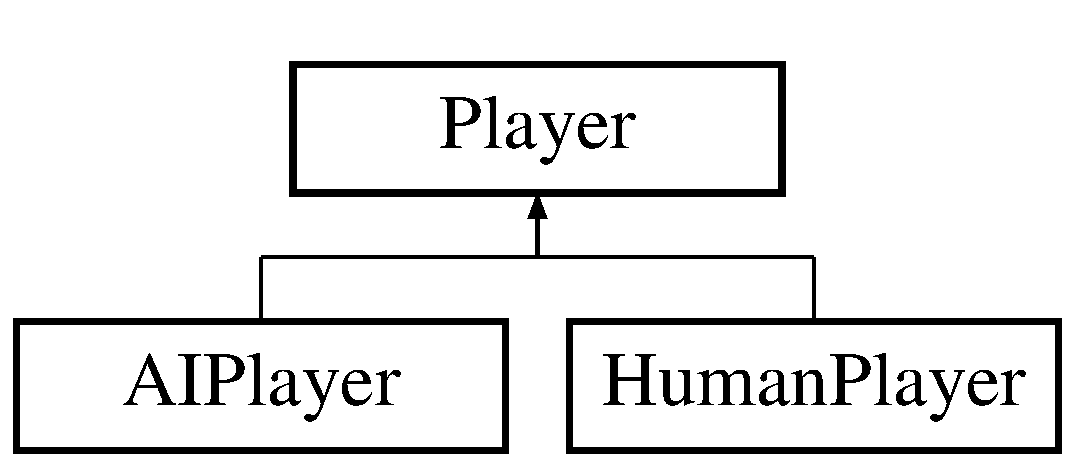
\includegraphics[height=2.000000cm]{class_player}
\end{center}
\end{figure}
\subsection*{Public Member Functions}
\begin{DoxyCompactItemize}
\item 
\hyperlink{class_player_ad079d0b82440f180a6698ff62f1dc1be}{Player} (Q\-String)
\begin{DoxyCompactList}\small\item\em \hyperlink{class_player_ad079d0b82440f180a6698ff62f1dc1be}{Player\-::\-Player} Constructor. \end{DoxyCompactList}\item 
virtual \hyperlink{class_player_a749d2c00e1fe0f5c2746f7505a58c062}{$\sim$\-Player} ()
\begin{DoxyCompactList}\small\item\em \hyperlink{class_player_a749d2c00e1fe0f5c2746f7505a58c062}{Player\-::$\sim$\-Player} Deconstructor. \end{DoxyCompactList}\item 
virtual bool \hyperlink{class_player_adeb8d6fe962f9bf002281f7fe1321cff}{is\-Human\-Player} ()
\begin{DoxyCompactList}\small\item\em \hyperlink{class_player_adeb8d6fe962f9bf002281f7fe1321cff}{Player\-::is\-Human\-Player}. \end{DoxyCompactList}\item 
virtual bool \hyperlink{class_player_afcd43a9498dc70a71ba17484699446bb}{is\-A\-I\-Player} ()
\begin{DoxyCompactList}\small\item\em \hyperlink{class_player_afcd43a9498dc70a71ba17484699446bb}{Player\-::is\-A\-I\-Player}. \end{DoxyCompactList}\item 
\hyperlink{class_player}{Player} $\ast$ \hyperlink{class_player_a720be779010f05b9af198db3e3181369}{remove\-Letter} (\hyperlink{class_letter}{Letter} $\ast$)
\begin{DoxyCompactList}\small\item\em \hyperlink{class_player_a720be779010f05b9af198db3e3181369}{Player\-::remove\-Letter} Removes the first letter that matches. \end{DoxyCompactList}\item 
\hyperlink{class_player}{Player} $\ast$ \hyperlink{class_player_afd0aad702c6ce04bed93c3349f10596f}{clear\-Letters} ()
\begin{DoxyCompactList}\small\item\em \hyperlink{class_player_afd0aad702c6ce04bed93c3349f10596f}{Player\-::clear\-Letters} Clears the player's letters. \end{DoxyCompactList}\item 
\hyperlink{class_player}{Player} $\ast$ \hyperlink{class_player_a78086401345079616a422c25cb780ecb}{get\-New\-Letters} (\hyperlink{class_letter_pool}{Letter\-Pool} $\ast$)
\begin{DoxyCompactList}\small\item\em \hyperlink{class_player_a78086401345079616a422c25cb780ecb}{Player\-::get\-New\-Letters} Fills the letters after a play. \end{DoxyCompactList}\item 
Q\-String $\ast$ \hyperlink{class_player_a2ca0e35ef05a2a14efab866f6cb32a76}{get\-Letters\-As\-Qstring} ()
\begin{DoxyCompactList}\small\item\em \hyperlink{class_player_a2ca0e35ef05a2a14efab866f6cb32a76}{Player\-::get\-Letters\-As\-Qstring} Gets the letters held as a string. \end{DoxyCompactList}\item 
\hyperlink{class_letter}{Letter} $\ast$ \hyperlink{class_player_aa6aabfbae536fec650fd466f65fb9743}{get\-Letter} (int)
\begin{DoxyCompactList}\small\item\em \hyperlink{class_player_aa6aabfbae536fec650fd466f65fb9743}{Player\-::get\-Letter} Getter for letter. \end{DoxyCompactList}\item 
void \hyperlink{class_player_a71fa8ceb20420f2c592b2fe7c50c3728}{fill\-Letters} (\hyperlink{class_letter_pool}{Letter\-Pool} $\ast$)
\begin{DoxyCompactList}\small\item\em Player\-::\-Requests for his letters to be filled out. \end{DoxyCompactList}\item 
int \hyperlink{class_player_a9def90c7578d965a506fe36d274b2403}{get\-Letter\-Count} ()
\begin{DoxyCompactList}\small\item\em \hyperlink{class_player_a9def90c7578d965a506fe36d274b2403}{Player\-::get\-Letter\-Count}. \end{DoxyCompactList}\item 
size\-\_\-t \hyperlink{class_player_a03398b3f33c323f4ad1eea16863e9a05}{add\-Letter} (\hyperlink{class_letter}{Letter} $\ast$letter)
\begin{DoxyCompactList}\small\item\em \hyperlink{class_player_a03398b3f33c323f4ad1eea16863e9a05}{Player\-::add\-Letter} Adds a letter to a players set of letters. \end{DoxyCompactList}\item 
Q\-String \hyperlink{class_player_ade0334ac0e87ac1c5e09ce78f2cafd83}{get\-Name} ()
\begin{DoxyCompactList}\small\item\em \hyperlink{class_player_ade0334ac0e87ac1c5e09ce78f2cafd83}{Player\-::get\-Name} Getter for name. \end{DoxyCompactList}\item 
int \hyperlink{class_player_aa5bead96a6eb9cc33fbc086662621caf}{add\-Score} (int)
\begin{DoxyCompactList}\small\item\em \hyperlink{class_player_aa5bead96a6eb9cc33fbc086662621caf}{Player\-::add\-Score} Adds to a player's score. \end{DoxyCompactList}\item 
void \hyperlink{class_player_a6e2f0837237f65c67948585ed2be56f9}{clear\-Score} ()
\begin{DoxyCompactList}\small\item\em \hyperlink{class_player_a6e2f0837237f65c67948585ed2be56f9}{Player\-::clear\-Score} Clears the \hyperlink{class_player}{Player}'s score. \end{DoxyCompactList}\item 
int \hyperlink{class_player_a97e5447778ae6c384eedc532dcd8431d}{get\-Score} ()
\begin{DoxyCompactList}\small\item\em \hyperlink{class_player_a97e5447778ae6c384eedc532dcd8431d}{Player\-::get\-Score} Gets a player's score. \end{DoxyCompactList}\end{DoxyCompactItemize}
\subsection*{Protected Attributes}
\begin{DoxyCompactItemize}
\item 
Q\-String \hyperlink{class_player_ac41b72814d9c41222dac999bc874280b}{name}
\item 
vector$<$ \hyperlink{class_letter}{Letter} $\ast$ $>$ \hyperlink{class_player_abd40dc8f6d524bd1331a8133e9bb8902}{letters}
\item 
unsigned int \hyperlink{class_player_a38a6dafe988a768a435cc0a9fde38e46}{score}
\end{DoxyCompactItemize}
\subsection*{Friends}
\begin{DoxyCompactItemize}
\item 
ostream \& \hyperlink{class_player_a79571356003607b80edc6440c851e503}{operator$<$$<$} (ostream \&os, const \hyperlink{class_player}{Player} \&player)
\begin{DoxyCompactList}\small\item\em operator $<$$<$ Overloaded operator for \hyperlink{class_player}{Player}\& \end{DoxyCompactList}\end{DoxyCompactItemize}


\subsection{Detailed Description}
The \hyperlink{class_player}{Player} class Abstract class representing a \hyperlink{class_player}{Player}. 

Definition at line 19 of file player.\-h.



\subsection{Constructor \& Destructor Documentation}
\hypertarget{class_player_ad079d0b82440f180a6698ff62f1dc1be}{\index{Player@{Player}!Player@{Player}}
\index{Player@{Player}!Player@{Player}}
\subsubsection[{Player}]{\setlength{\rightskip}{0pt plus 5cm}Player\-::\-Player (
\begin{DoxyParamCaption}
\item[{Q\-String}]{name}
\end{DoxyParamCaption}
)}}\label{class_player_ad079d0b82440f180a6698ff62f1dc1be}


\hyperlink{class_player_ad079d0b82440f180a6698ff62f1dc1be}{Player\-::\-Player} Constructor. 


\begin{DoxyParams}{Parameters}
{\em name} & \\
\hline
\end{DoxyParams}


Definition at line 8 of file player.\-cpp.



References letters, name, and score.


\begin{DoxyCode}
9 \{
10     this->\hyperlink{class_player_ac41b72814d9c41222dac999bc874280b}{name} = \hyperlink{class_player_ac41b72814d9c41222dac999bc874280b}{name};
11     this->\hyperlink{class_player_a38a6dafe988a768a435cc0a9fde38e46}{score} = 0;
12     this->\hyperlink{class_player_abd40dc8f6d524bd1331a8133e9bb8902}{letters}.reserve(7);
13 \}
\end{DoxyCode}
\hypertarget{class_player_a749d2c00e1fe0f5c2746f7505a58c062}{\index{Player@{Player}!$\sim$\-Player@{$\sim$\-Player}}
\index{$\sim$\-Player@{$\sim$\-Player}!Player@{Player}}
\subsubsection[{$\sim$\-Player}]{\setlength{\rightskip}{0pt plus 5cm}Player\-::$\sim$\-Player (
\begin{DoxyParamCaption}
{}
\end{DoxyParamCaption}
)\hspace{0.3cm}{\ttfamily [virtual]}}}\label{class_player_a749d2c00e1fe0f5c2746f7505a58c062}


\hyperlink{class_player_a749d2c00e1fe0f5c2746f7505a58c062}{Player\-::$\sim$\-Player} Deconstructor. 



Definition at line 18 of file player.\-cpp.


\begin{DoxyCode}
19 \{
20 
21 \}
\end{DoxyCode}


\subsection{Member Function Documentation}
\hypertarget{class_player_a03398b3f33c323f4ad1eea16863e9a05}{\index{Player@{Player}!add\-Letter@{add\-Letter}}
\index{add\-Letter@{add\-Letter}!Player@{Player}}
\subsubsection[{add\-Letter}]{\setlength{\rightskip}{0pt plus 5cm}size\-\_\-t Player\-::add\-Letter (
\begin{DoxyParamCaption}
\item[{{\bf Letter} $\ast$}]{letter}
\end{DoxyParamCaption}
)}}\label{class_player_a03398b3f33c323f4ad1eea16863e9a05}


\hyperlink{class_player_a03398b3f33c323f4ad1eea16863e9a05}{Player\-::add\-Letter} Adds a letter to a players set of letters. 


\begin{DoxyParams}{Parameters}
{\em letter} & The letter to add \\
\hline
\end{DoxyParams}
\begin{DoxyReturn}{Returns}
On sucess a positive integer of the number of tiles held, on failure -\/1 
\end{DoxyReturn}


Definition at line 55 of file player.\-cpp.



References letters, and M\-A\-X\-T\-I\-L\-E\-S\-I\-N\-H\-A\-N\-D.


\begin{DoxyCode}
55                                        \{
56     \textcolor{keywordflow}{if} (\hyperlink{class_player_abd40dc8f6d524bd1331a8133e9bb8902}{letters}.size() < (\hyperlink{player_8h_a65437be5d7abb586fe7338331e988e01}{MAXTILESINHAND} - 1))\{
57         \hyperlink{class_player_abd40dc8f6d524bd1331a8133e9bb8902}{letters}.push\_back(letter);
58         \textcolor{keywordflow}{return} \hyperlink{class_player_abd40dc8f6d524bd1331a8133e9bb8902}{letters}.size();
59     \}
60 
61     \textcolor{keywordflow}{return} -1;
62 \}
\end{DoxyCode}
\hypertarget{class_player_aa5bead96a6eb9cc33fbc086662621caf}{\index{Player@{Player}!add\-Score@{add\-Score}}
\index{add\-Score@{add\-Score}!Player@{Player}}
\subsubsection[{add\-Score}]{\setlength{\rightskip}{0pt plus 5cm}int Player\-::add\-Score (
\begin{DoxyParamCaption}
\item[{int}]{new\-Score}
\end{DoxyParamCaption}
)}}\label{class_player_aa5bead96a6eb9cc33fbc086662621caf}


\hyperlink{class_player_aa5bead96a6eb9cc33fbc086662621caf}{Player\-::add\-Score} Adds to a player's score. 


\begin{DoxyParams}{Parameters}
{\em new\-Score} & The amount to add \\
\hline
\end{DoxyParams}
\begin{DoxyReturn}{Returns}
The modified score 
\end{DoxyReturn}


Definition at line 136 of file player.\-cpp.



References score.



Referenced by Game\-::next\-Turn().


\begin{DoxyCode}
136                                  \{
137     this->\hyperlink{class_player_a38a6dafe988a768a435cc0a9fde38e46}{score} += newScore;
138 
139     \textcolor{keywordflow}{return} this->\hyperlink{class_player_a38a6dafe988a768a435cc0a9fde38e46}{score};
140 \}
\end{DoxyCode}
\hypertarget{class_player_afd0aad702c6ce04bed93c3349f10596f}{\index{Player@{Player}!clear\-Letters@{clear\-Letters}}
\index{clear\-Letters@{clear\-Letters}!Player@{Player}}
\subsubsection[{clear\-Letters}]{\setlength{\rightskip}{0pt plus 5cm}{\bf Player} $\ast$ Player\-::clear\-Letters (
\begin{DoxyParamCaption}
{}
\end{DoxyParamCaption}
)}}\label{class_player_afd0aad702c6ce04bed93c3349f10596f}


\hyperlink{class_player_afd0aad702c6ce04bed93c3349f10596f}{Player\-::clear\-Letters} Clears the player's letters. 

\begin{DoxyReturn}{Returns}
this 
\end{DoxyReturn}


Definition at line 174 of file player.\-cpp.



References letters.


\begin{DoxyCode}
174                             \{
175     \textcolor{keywordflow}{while}(!\hyperlink{class_player_abd40dc8f6d524bd1331a8133e9bb8902}{letters}.empty())\{
176         \textcolor{keyword}{delete} \hyperlink{class_player_abd40dc8f6d524bd1331a8133e9bb8902}{letters}.back();
177         \hyperlink{class_player_abd40dc8f6d524bd1331a8133e9bb8902}{letters}.pop\_back();
178     \}
179     \textcolor{keywordflow}{return} \textcolor{keyword}{this};
180 \}
\end{DoxyCode}
\hypertarget{class_player_a6e2f0837237f65c67948585ed2be56f9}{\index{Player@{Player}!clear\-Score@{clear\-Score}}
\index{clear\-Score@{clear\-Score}!Player@{Player}}
\subsubsection[{clear\-Score}]{\setlength{\rightskip}{0pt plus 5cm}void Player\-::clear\-Score (
\begin{DoxyParamCaption}
{}
\end{DoxyParamCaption}
)}}\label{class_player_a6e2f0837237f65c67948585ed2be56f9}


\hyperlink{class_player_a6e2f0837237f65c67948585ed2be56f9}{Player\-::clear\-Score} Clears the \hyperlink{class_player}{Player}'s score. 



Definition at line 145 of file player.\-cpp.



References score.


\begin{DoxyCode}
146 \{
147     this->\hyperlink{class_player_a38a6dafe988a768a435cc0a9fde38e46}{score} = 0;
148 \}
\end{DoxyCode}
\hypertarget{class_player_a71fa8ceb20420f2c592b2fe7c50c3728}{\index{Player@{Player}!fill\-Letters@{fill\-Letters}}
\index{fill\-Letters@{fill\-Letters}!Player@{Player}}
\subsubsection[{fill\-Letters}]{\setlength{\rightskip}{0pt plus 5cm}void Player\-::fill\-Letters (
\begin{DoxyParamCaption}
\item[{{\bf Letter\-Pool} $\ast$}]{pool}
\end{DoxyParamCaption}
)}}\label{class_player_a71fa8ceb20420f2c592b2fe7c50c3728}


Player\-::\-Requests for his letters to be filled out. 



Definition at line 162 of file player.\-cpp.



References Letter\-Pool\-::get\-Random\-Letter(), Letter\-Pool\-::is\-Empty(), letters, and M\-A\-X\-T\-I\-L\-E\-S\-I\-N\-H\-A\-N\-D.



Referenced by get\-New\-Letters().


\begin{DoxyCode}
162                                         \{
163 
164     \textcolor{keywordflow}{while}(!pool->\hyperlink{class_letter_pool_a47817d0343b330f2c6f3413288de69b2}{isEmpty}() && \hyperlink{class_player_abd40dc8f6d524bd1331a8133e9bb8902}{letters}.size() < \hyperlink{player_8h_a65437be5d7abb586fe7338331e988e01}{MAXTILESINHAND})
165     \{
166            \hyperlink{class_player_abd40dc8f6d524bd1331a8133e9bb8902}{letters}.push\_back(pool->\hyperlink{class_letter_pool_acf36848e6c23f40de9b98f43755d586c}{getRandomLetter}());
167     \}
168 \}
\end{DoxyCode}
\hypertarget{class_player_aa6aabfbae536fec650fd466f65fb9743}{\index{Player@{Player}!get\-Letter@{get\-Letter}}
\index{get\-Letter@{get\-Letter}!Player@{Player}}
\subsubsection[{get\-Letter}]{\setlength{\rightskip}{0pt plus 5cm}{\bf Letter} $\ast$ Player\-::get\-Letter (
\begin{DoxyParamCaption}
\item[{int}]{i}
\end{DoxyParamCaption}
)}}\label{class_player_aa6aabfbae536fec650fd466f65fb9743}


\hyperlink{class_player_aa6aabfbae536fec650fd466f65fb9743}{Player\-::get\-Letter} Getter for letter. 


\begin{DoxyParams}{Parameters}
{\em i} & The index of the letter \\
\hline
\end{DoxyParams}
\begin{DoxyReturn}{Returns}
A pointer to the letter or N\-U\-L\-L if it doesn't exist 
\end{DoxyReturn}


Definition at line 111 of file player.\-cpp.



References letters.



Referenced by Rack\-::refresh().


\begin{DoxyCode}
111                               \{
112     \textcolor{keywordflow}{if} (i >= 0 && (\textcolor{keywordtype}{unsigned} \textcolor{keywordtype}{int})i < \hyperlink{class_player_abd40dc8f6d524bd1331a8133e9bb8902}{letters}.size())\{
113         \textcolor{keywordflow}{return} \hyperlink{class_player_abd40dc8f6d524bd1331a8133e9bb8902}{letters}.at(i);
114     \}
115     \textcolor{keywordflow}{return} NULL;
116 \}
\end{DoxyCode}
\hypertarget{class_player_a9def90c7578d965a506fe36d274b2403}{\index{Player@{Player}!get\-Letter\-Count@{get\-Letter\-Count}}
\index{get\-Letter\-Count@{get\-Letter\-Count}!Player@{Player}}
\subsubsection[{get\-Letter\-Count}]{\setlength{\rightskip}{0pt plus 5cm}int Player\-::get\-Letter\-Count (
\begin{DoxyParamCaption}
{}
\end{DoxyParamCaption}
)}}\label{class_player_a9def90c7578d965a506fe36d274b2403}


\hyperlink{class_player_a9def90c7578d965a506fe36d274b2403}{Player\-::get\-Letter\-Count}. 

\begin{DoxyReturn}{Returns}
Returns the number of letter in players hand for debugging purposes mostly 
\end{DoxyReturn}


Definition at line 28 of file player.\-cpp.



References letters.


\begin{DoxyCode}
28                           \{
29     \textcolor{keywordflow}{return} (\textcolor{keywordtype}{int})\hyperlink{class_player_abd40dc8f6d524bd1331a8133e9bb8902}{letters}.size();
30 \}
\end{DoxyCode}
\hypertarget{class_player_a2ca0e35ef05a2a14efab866f6cb32a76}{\index{Player@{Player}!get\-Letters\-As\-Qstring@{get\-Letters\-As\-Qstring}}
\index{get\-Letters\-As\-Qstring@{get\-Letters\-As\-Qstring}!Player@{Player}}
\subsubsection[{get\-Letters\-As\-Qstring}]{\setlength{\rightskip}{0pt plus 5cm}Q\-String $\ast$ Player\-::get\-Letters\-As\-Qstring (
\begin{DoxyParamCaption}
{}
\end{DoxyParamCaption}
)}}\label{class_player_a2ca0e35ef05a2a14efab866f6cb32a76}


\hyperlink{class_player_a2ca0e35ef05a2a14efab866f6cb32a76}{Player\-::get\-Letters\-As\-Qstring} Gets the letters held as a string. 

\begin{DoxyReturn}{Returns}
A Q\-String representing the letters held 
\end{DoxyReturn}


Definition at line 122 of file player.\-cpp.



References letters.


\begin{DoxyCode}
122                                     \{
123     \textcolor{keywordtype}{size\_t} numLetters = \hyperlink{class_player_abd40dc8f6d524bd1331a8133e9bb8902}{letters}.size();
124     QString *qstring = \textcolor{keyword}{new} QString;
125     \textcolor{keywordflow}{for}(\textcolor{keywordtype}{size\_t} i = 0; i < numLetters; i++)\{
126         qstring->push\_back(*(\hyperlink{class_player_abd40dc8f6d524bd1331a8133e9bb8902}{letters}[i]->asQCharPtr()));
127     \}
128     \textcolor{keywordflow}{return} qstring;
129 \}
\end{DoxyCode}
\hypertarget{class_player_ade0334ac0e87ac1c5e09ce78f2cafd83}{\index{Player@{Player}!get\-Name@{get\-Name}}
\index{get\-Name@{get\-Name}!Player@{Player}}
\subsubsection[{get\-Name}]{\setlength{\rightskip}{0pt plus 5cm}Q\-String Player\-::get\-Name (
\begin{DoxyParamCaption}
{}
\end{DoxyParamCaption}
)}}\label{class_player_ade0334ac0e87ac1c5e09ce78f2cafd83}


\hyperlink{class_player_ade0334ac0e87ac1c5e09ce78f2cafd83}{Player\-::get\-Name} Getter for name. 

\begin{DoxyReturn}{Returns}
name 
\end{DoxyReturn}


Definition at line 100 of file player.\-cpp.



References name.



Referenced by Player\-Label\-::update\-Text().


\begin{DoxyCode}
101 \{
102     \textcolor{keywordflow}{return} \hyperlink{class_player_ac41b72814d9c41222dac999bc874280b}{name};
103 \}
\end{DoxyCode}
\hypertarget{class_player_a78086401345079616a422c25cb780ecb}{\index{Player@{Player}!get\-New\-Letters@{get\-New\-Letters}}
\index{get\-New\-Letters@{get\-New\-Letters}!Player@{Player}}
\subsubsection[{get\-New\-Letters}]{\setlength{\rightskip}{0pt plus 5cm}{\bf Player} $\ast$ Player\-::get\-New\-Letters (
\begin{DoxyParamCaption}
\item[{{\bf Letter\-Pool} $\ast$}]{pool}
\end{DoxyParamCaption}
)}}\label{class_player_a78086401345079616a422c25cb780ecb}


\hyperlink{class_player_a78086401345079616a422c25cb780ecb}{Player\-::get\-New\-Letters} Fills the letters after a play. 


\begin{DoxyParams}{Parameters}
{\em pool} & The letter pool \\
\hline
\end{DoxyParams}
\begin{DoxyReturn}{Returns}
this 
\end{DoxyReturn}
\begin{DoxyRefDesc}{Todo}
\item[\hyperlink{todo__todo000003}{Todo}]this is a bug , it removes the first letter regardless \end{DoxyRefDesc}


Definition at line 84 of file player.\-cpp.



References fill\-Letters(), Rack\-::get\-Rack(), letters, and R\-A\-C\-K\-S\-I\-Z\-E.



Referenced by Game\-::next\-Turn().


\begin{DoxyCode}
85 \{
86     \textcolor{keywordflow}{for}(\textcolor{keywordtype}{int} i = \hyperlink{rack_8h_ad52276b6cc76ff4be1f71000a9094f31}{RACKSIZE} - 1; i >= 0; i--)\{
87         \textcolor{keywordflow}{if} (\hyperlink{class_rack_aa48de650c15bda8267451d84caf6ea3f}{Rack::getRack}()->getSpace(i)->isPlaced())\{
89             \hyperlink{class_player_abd40dc8f6d524bd1331a8133e9bb8902}{letters}.erase(\hyperlink{class_player_abd40dc8f6d524bd1331a8133e9bb8902}{letters}.begin() + i);
90         \}
91     \}
92     \hyperlink{class_player_a71fa8ceb20420f2c592b2fe7c50c3728}{fillLetters}(pool);
93     \textcolor{keywordflow}{return} \textcolor{keyword}{this};
94 \}
\end{DoxyCode}
\hypertarget{class_player_a97e5447778ae6c384eedc532dcd8431d}{\index{Player@{Player}!get\-Score@{get\-Score}}
\index{get\-Score@{get\-Score}!Player@{Player}}
\subsubsection[{get\-Score}]{\setlength{\rightskip}{0pt plus 5cm}int Player\-::get\-Score (
\begin{DoxyParamCaption}
{}
\end{DoxyParamCaption}
)}}\label{class_player_a97e5447778ae6c384eedc532dcd8431d}


\hyperlink{class_player_a97e5447778ae6c384eedc532dcd8431d}{Player\-::get\-Score} Gets a player's score. 

\begin{DoxyReturn}{Returns}
The player's score 
\end{DoxyReturn}


Definition at line 154 of file player.\-cpp.



References score.



Referenced by Player\-Label\-::update\-Text().


\begin{DoxyCode}
154                      \{
155     \textcolor{keywordflow}{return} this->\hyperlink{class_player_a38a6dafe988a768a435cc0a9fde38e46}{score};
156 \}
\end{DoxyCode}
\hypertarget{class_player_afcd43a9498dc70a71ba17484699446bb}{\index{Player@{Player}!is\-A\-I\-Player@{is\-A\-I\-Player}}
\index{is\-A\-I\-Player@{is\-A\-I\-Player}!Player@{Player}}
\subsubsection[{is\-A\-I\-Player}]{\setlength{\rightskip}{0pt plus 5cm}bool Player\-::is\-A\-I\-Player (
\begin{DoxyParamCaption}
{}
\end{DoxyParamCaption}
)\hspace{0.3cm}{\ttfamily [virtual]}}}\label{class_player_afcd43a9498dc70a71ba17484699446bb}


\hyperlink{class_player_afcd43a9498dc70a71ba17484699446bb}{Player\-::is\-A\-I\-Player}. 

\begin{DoxyReturn}{Returns}
True if an A\-I player, false otherwise 
\end{DoxyReturn}


Reimplemented in \hyperlink{class_a_i_player_a2a71a31297386f4d69f12a43187954a6}{A\-I\-Player}.



Definition at line 45 of file player.\-cpp.


\begin{DoxyCode}
45                        \{
46     \textcolor{keywordflow}{return} \textcolor{keyword}{false};
47 \}
\end{DoxyCode}
\hypertarget{class_player_adeb8d6fe962f9bf002281f7fe1321cff}{\index{Player@{Player}!is\-Human\-Player@{is\-Human\-Player}}
\index{is\-Human\-Player@{is\-Human\-Player}!Player@{Player}}
\subsubsection[{is\-Human\-Player}]{\setlength{\rightskip}{0pt plus 5cm}bool Player\-::is\-Human\-Player (
\begin{DoxyParamCaption}
{}
\end{DoxyParamCaption}
)\hspace{0.3cm}{\ttfamily [virtual]}}}\label{class_player_adeb8d6fe962f9bf002281f7fe1321cff}


\hyperlink{class_player_adeb8d6fe962f9bf002281f7fe1321cff}{Player\-::is\-Human\-Player}. 

\begin{DoxyReturn}{Returns}
True if a human player, false otherwise 
\end{DoxyReturn}


Reimplemented in \hyperlink{class_human_player_aff784db8904c5f8c13bd88847f631188}{Human\-Player}.



Definition at line 36 of file player.\-cpp.


\begin{DoxyCode}
37 \{
38     \textcolor{keywordflow}{return} \textcolor{keyword}{false};
39 \}
\end{DoxyCode}
\hypertarget{class_player_a720be779010f05b9af198db3e3181369}{\index{Player@{Player}!remove\-Letter@{remove\-Letter}}
\index{remove\-Letter@{remove\-Letter}!Player@{Player}}
\subsubsection[{remove\-Letter}]{\setlength{\rightskip}{0pt plus 5cm}{\bf Player} $\ast$ Player\-::remove\-Letter (
\begin{DoxyParamCaption}
\item[{{\bf Letter} $\ast$}]{letter}
\end{DoxyParamCaption}
)}}\label{class_player_a720be779010f05b9af198db3e3181369}


\hyperlink{class_player_a720be779010f05b9af198db3e3181369}{Player\-::remove\-Letter} Removes the first letter that matches. 


\begin{DoxyParams}{Parameters}
{\em letter} & The letter to remove \\
\hline
\end{DoxyParams}
\begin{DoxyReturn}{Returns}
A pointer to the letter object, or N\-U\-L\-L if not found 
\end{DoxyReturn}


Definition at line 69 of file player.\-cpp.



References letters.


\begin{DoxyCode}
69                                            \{
70     \textcolor{keywordtype}{size\_t} numLetters = \hyperlink{class_player_abd40dc8f6d524bd1331a8133e9bb8902}{letters}.size();
71     \textcolor{keywordflow}{for}(\textcolor{keywordtype}{size\_t} i = 0; i < numLetters; i++)\{
72         \textcolor{keywordflow}{if} (\hyperlink{class_player_abd40dc8f6d524bd1331a8133e9bb8902}{letters}[i] == letter)\{
73             \hyperlink{class_player_abd40dc8f6d524bd1331a8133e9bb8902}{letters}.erase(\hyperlink{class_player_abd40dc8f6d524bd1331a8133e9bb8902}{letters}.begin() + i);
74         \}
75     \}
76     \textcolor{keywordflow}{return} \textcolor{keyword}{this};
77 \}
\end{DoxyCode}


\subsection{Friends And Related Function Documentation}
\hypertarget{class_player_a79571356003607b80edc6440c851e503}{\index{Player@{Player}!operator$<$$<$@{operator$<$$<$}}
\index{operator$<$$<$@{operator$<$$<$}!Player@{Player}}
\subsubsection[{operator$<$$<$}]{\setlength{\rightskip}{0pt plus 5cm}ostream\& operator$<$$<$ (
\begin{DoxyParamCaption}
\item[{ostream \&}]{os, }
\item[{const {\bf Player} \&}]{player}
\end{DoxyParamCaption}
)\hspace{0.3cm}{\ttfamily [friend]}}}\label{class_player_a79571356003607b80edc6440c851e503}


operator $<$$<$ Overloaded operator for \hyperlink{class_player}{Player}\& 


\begin{DoxyParams}{Parameters}
{\em os} & The ostream \\
\hline
{\em player} & The player \\
\hline
\end{DoxyParams}
\begin{DoxyReturn}{Returns}
The modified ostream 
\end{DoxyReturn}


Definition at line 188 of file player.\-cpp.


\begin{DoxyCode}
188                                                        \{
189     \textcolor{keywordflow}{for}(\textcolor{keywordtype}{unsigned} \textcolor{keywordtype}{int} i = 0; i < player.\hyperlink{class_player_abd40dc8f6d524bd1331a8133e9bb8902}{letters}.size(); i++) \{
190         os << *(player.\hyperlink{class_player_abd40dc8f6d524bd1331a8133e9bb8902}{letters}[i]);
191     \}
192     \textcolor{keywordflow}{return} os;
193 \}
\end{DoxyCode}


\subsection{Member Data Documentation}
\hypertarget{class_player_abd40dc8f6d524bd1331a8133e9bb8902}{\index{Player@{Player}!letters@{letters}}
\index{letters@{letters}!Player@{Player}}
\subsubsection[{letters}]{\setlength{\rightskip}{0pt plus 5cm}vector$<${\bf Letter}$\ast$$>$ Player\-::letters\hspace{0.3cm}{\ttfamily [protected]}}}\label{class_player_abd40dc8f6d524bd1331a8133e9bb8902}
The Letters the \hyperlink{class_player}{Player} has 

Definition at line 23 of file player.\-h.



Referenced by add\-Letter(), clear\-Letters(), fill\-Letters(), get\-Letter(), get\-Letter\-Count(), get\-Letters\-As\-Qstring(), get\-New\-Letters(), operator$<$$<$(), A\-I\-Player\-::play(), Player(), remove\-Letter(), and Human\-Player\-::$\sim$\-Human\-Player().

\hypertarget{class_player_ac41b72814d9c41222dac999bc874280b}{\index{Player@{Player}!name@{name}}
\index{name@{name}!Player@{Player}}
\subsubsection[{name}]{\setlength{\rightskip}{0pt plus 5cm}Q\-String Player\-::name\hspace{0.3cm}{\ttfamily [protected]}}}\label{class_player_ac41b72814d9c41222dac999bc874280b}
The \hyperlink{class_player}{Player}'s name 

Definition at line 22 of file player.\-h.



Referenced by get\-Name(), and Player().

\hypertarget{class_player_a38a6dafe988a768a435cc0a9fde38e46}{\index{Player@{Player}!score@{score}}
\index{score@{score}!Player@{Player}}
\subsubsection[{score}]{\setlength{\rightskip}{0pt plus 5cm}unsigned int Player\-::score\hspace{0.3cm}{\ttfamily [protected]}}}\label{class_player_a38a6dafe988a768a435cc0a9fde38e46}
The \hyperlink{class_player}{Player}'s score 

Definition at line 24 of file player.\-h.



Referenced by add\-Score(), clear\-Score(), get\-Score(), and Player().



The documentation for this class was generated from the following files\-:\begin{DoxyCompactItemize}
\item 
Scrabble/\hyperlink{player_8h}{player.\-h}\item 
Scrabble/\hyperlink{player_8cpp}{player.\-cpp}\end{DoxyCompactItemize}

\hypertarget{class_player_label}{\section{Player\-Label Class Reference}
\label{class_player_label}\index{Player\-Label@{Player\-Label}}
}


The \hyperlink{class_player_label}{Player\-Label} class Represents the \hyperlink{class_player}{Player} within the \hyperlink{class_dialog}{Dialog}.  




{\ttfamily \#include $<$playerlabel.\-h$>$}

Inheritance diagram for Player\-Label\-:\begin{figure}[H]
\begin{center}
\leavevmode
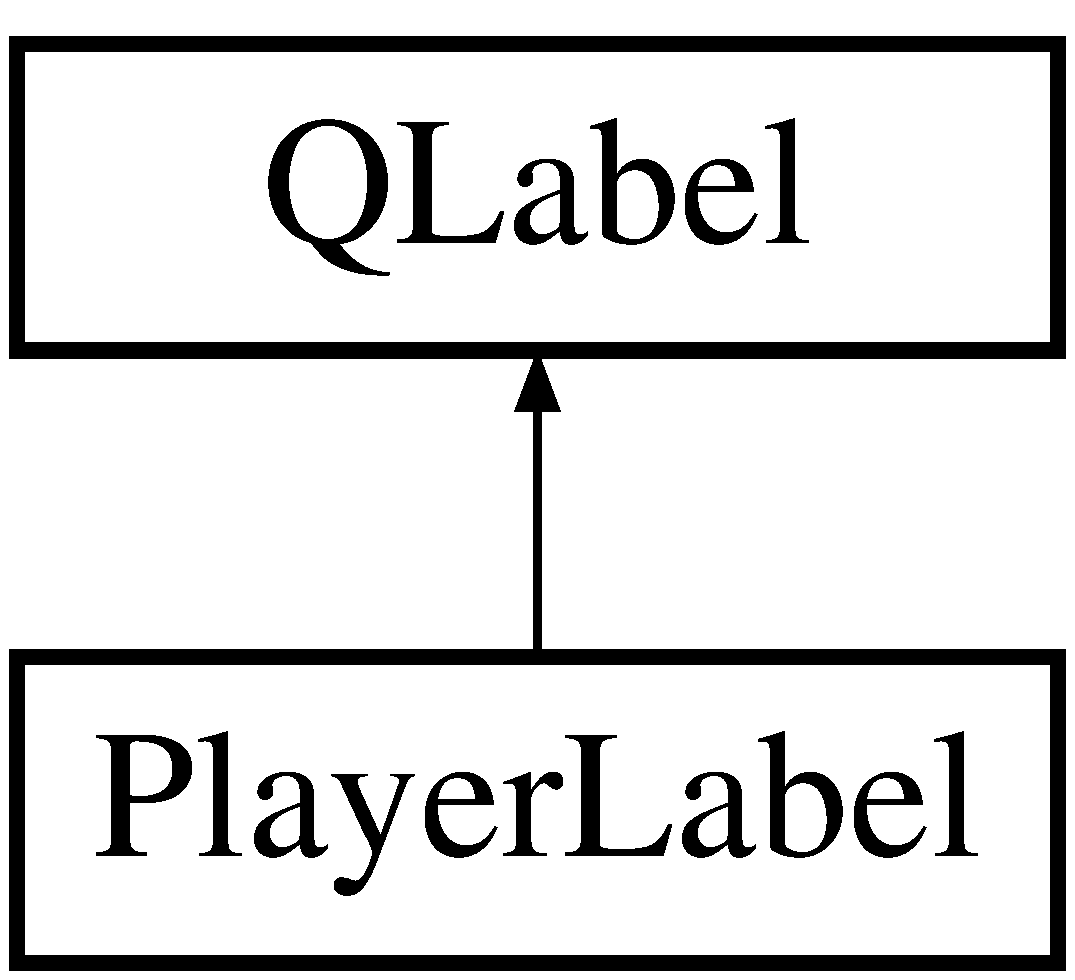
\includegraphics[height=2.000000cm]{class_player_label}
\end{center}
\end{figure}
\subsection*{Public Slots}
\begin{DoxyCompactItemize}
\item 
void \hyperlink{class_player_label_a4e79270b2cc5ae00ff3ea5e648d48e0a}{on\-\_\-player\-Changed} ()
\begin{DoxyCompactList}\small\item\em \hyperlink{class_player_label_a4e79270b2cc5ae00ff3ea5e648d48e0a}{Player\-Label\-::on\-\_\-player\-Changed} Handes player\-Changed events. \end{DoxyCompactList}\end{DoxyCompactItemize}
\subsection*{Public Member Functions}
\begin{DoxyCompactItemize}
\item 
\hyperlink{class_player_label_a01014b0be21549ebd1fcec81fa8d6d58}{Player\-Label} (\hyperlink{class_player}{Player} $\ast$)
\begin{DoxyCompactList}\small\item\em \hyperlink{class_player_label_a01014b0be21549ebd1fcec81fa8d6d58}{Player\-Label\-::\-Player\-Label} Constructor. \end{DoxyCompactList}\item 
\hyperlink{class_player_label}{Player\-Label} $\ast$ \hyperlink{class_player_label_a2dfa25456fac3bd2f0a7bbaa4fac6678}{set\-Active} ()
\begin{DoxyCompactList}\small\item\em \hyperlink{class_player_label_a2dfa25456fac3bd2f0a7bbaa4fac6678}{Player\-Label\-::set\-Active} Sets the player as active. \end{DoxyCompactList}\item 
\hyperlink{class_player_label}{Player\-Label} $\ast$ \hyperlink{class_player_label_aecd91b6a5f19cd8228869a23bdb7da02}{set\-Inactive} ()
\begin{DoxyCompactList}\small\item\em \hyperlink{class_player_label_aecd91b6a5f19cd8228869a23bdb7da02}{Player\-Label\-::set\-Inactive} Set the player as inactive. \end{DoxyCompactList}\end{DoxyCompactItemize}
\subsection*{Private Member Functions}
\begin{DoxyCompactItemize}
\item 
\hyperlink{class_player_label}{Player\-Label} $\ast$ \hyperlink{class_player_label_a32738e0f6917a3942dd12569bb32ddd3}{update\-Text} ()
\begin{DoxyCompactList}\small\item\em \hyperlink{class_player_label_a32738e0f6917a3942dd12569bb32ddd3}{Player\-Label\-::update\-Text} Updates the text. \end{DoxyCompactList}\end{DoxyCompactItemize}
\subsection*{Private Attributes}
\begin{DoxyCompactItemize}
\item 
\hyperlink{class_player}{Player} $\ast$ \hyperlink{class_player_label_a3d7bf640f27b4539cb6886e53900b5b2}{player}
\end{DoxyCompactItemize}


\subsection{Detailed Description}
The \hyperlink{class_player_label}{Player\-Label} class Represents the \hyperlink{class_player}{Player} within the \hyperlink{class_dialog}{Dialog}. 

Definition at line 10 of file playerlabel.\-h.



\subsection{Constructor \& Destructor Documentation}
\hypertarget{class_player_label_a01014b0be21549ebd1fcec81fa8d6d58}{\index{Player\-Label@{Player\-Label}!Player\-Label@{Player\-Label}}
\index{Player\-Label@{Player\-Label}!PlayerLabel@{Player\-Label}}
\subsubsection[{Player\-Label}]{\setlength{\rightskip}{0pt plus 5cm}Player\-Label\-::\-Player\-Label (
\begin{DoxyParamCaption}
\item[{{\bf Player} $\ast$}]{player}
\end{DoxyParamCaption}
)\hspace{0.3cm}{\ttfamily [explicit]}}}\label{class_player_label_a01014b0be21549ebd1fcec81fa8d6d58}


\hyperlink{class_player_label_a01014b0be21549ebd1fcec81fa8d6d58}{Player\-Label\-::\-Player\-Label} Constructor. 


\begin{DoxyParams}{Parameters}
{\em player} & \\
\hline
\end{DoxyParams}


Definition at line 7 of file playerlabel.\-cpp.



References player.


\begin{DoxyCode}
7                                        :
8     QLabel()
9 \{
10     this->player = \hyperlink{class_player_label_a3d7bf640f27b4539cb6886e53900b5b2}{player};
11 \}
\end{DoxyCode}


\subsection{Member Function Documentation}
\hypertarget{class_player_label_a4e79270b2cc5ae00ff3ea5e648d48e0a}{\index{Player\-Label@{Player\-Label}!on\-\_\-player\-Changed@{on\-\_\-player\-Changed}}
\index{on\-\_\-player\-Changed@{on\-\_\-player\-Changed}!PlayerLabel@{Player\-Label}}
\subsubsection[{on\-\_\-player\-Changed}]{\setlength{\rightskip}{0pt plus 5cm}void Player\-Label\-::on\-\_\-player\-Changed (
\begin{DoxyParamCaption}
{}
\end{DoxyParamCaption}
)\hspace{0.3cm}{\ttfamily [slot]}}}\label{class_player_label_a4e79270b2cc5ae00ff3ea5e648d48e0a}


\hyperlink{class_player_label_a4e79270b2cc5ae00ff3ea5e648d48e0a}{Player\-Label\-::on\-\_\-player\-Changed} Handes player\-Changed events. 



Definition at line 16 of file playerlabel.\-cpp.



References Board\-::get\-Board(), player, set\-Active(), set\-Inactive(), and update\-Text().


\begin{DoxyCode}
17 \{
18     \textcolor{keywordflow}{if} (\hyperlink{class_player_label_a3d7bf640f27b4539cb6886e53900b5b2}{player} == \hyperlink{class_board_ae30e802b1d83309fc95e695b5b3df338}{Board::getBoard}()->getGame()->currentPlayer())\{
19         \hyperlink{class_player_label_a32738e0f6917a3942dd12569bb32ddd3}{updateText}();
20         \hyperlink{class_player_label_a2dfa25456fac3bd2f0a7bbaa4fac6678}{setActive}();
21     \}
22     \textcolor{keywordflow}{else} \{
23         \hyperlink{class_player_label_a32738e0f6917a3942dd12569bb32ddd3}{updateText}();
24         \hyperlink{class_player_label_aecd91b6a5f19cd8228869a23bdb7da02}{setInactive}();
25     \}
26 \}
\end{DoxyCode}
\hypertarget{class_player_label_a2dfa25456fac3bd2f0a7bbaa4fac6678}{\index{Player\-Label@{Player\-Label}!set\-Active@{set\-Active}}
\index{set\-Active@{set\-Active}!PlayerLabel@{Player\-Label}}
\subsubsection[{set\-Active}]{\setlength{\rightskip}{0pt plus 5cm}{\bf Player\-Label} $\ast$ Player\-Label\-::set\-Active (
\begin{DoxyParamCaption}
{}
\end{DoxyParamCaption}
)}}\label{class_player_label_a2dfa25456fac3bd2f0a7bbaa4fac6678}


\hyperlink{class_player_label_a2dfa25456fac3bd2f0a7bbaa4fac6678}{Player\-Label\-::set\-Active} Sets the player as active. 

\begin{DoxyReturn}{Returns}
this 
\end{DoxyReturn}


Definition at line 32 of file playerlabel.\-cpp.



References update\-Text().



Referenced by Dialog\-::create\-Label\-Group\-Box(), and on\-\_\-player\-Changed().


\begin{DoxyCode}
33 \{
34     \hyperlink{class_player_label_a32738e0f6917a3942dd12569bb32ddd3}{updateText}();
35     this->setStyleSheet(\textcolor{stringliteral}{"QLabel \{ color : red; \}"});
36     \textcolor{keywordflow}{return} \textcolor{keyword}{this};
37 \}
\end{DoxyCode}
\hypertarget{class_player_label_aecd91b6a5f19cd8228869a23bdb7da02}{\index{Player\-Label@{Player\-Label}!set\-Inactive@{set\-Inactive}}
\index{set\-Inactive@{set\-Inactive}!PlayerLabel@{Player\-Label}}
\subsubsection[{set\-Inactive}]{\setlength{\rightskip}{0pt plus 5cm}{\bf Player\-Label} $\ast$ Player\-Label\-::set\-Inactive (
\begin{DoxyParamCaption}
{}
\end{DoxyParamCaption}
)}}\label{class_player_label_aecd91b6a5f19cd8228869a23bdb7da02}


\hyperlink{class_player_label_aecd91b6a5f19cd8228869a23bdb7da02}{Player\-Label\-::set\-Inactive} Set the player as inactive. 

\begin{DoxyReturn}{Returns}
this 
\end{DoxyReturn}


Definition at line 43 of file playerlabel.\-cpp.



References update\-Text().



Referenced by Dialog\-::create\-Label\-Group\-Box(), and on\-\_\-player\-Changed().


\begin{DoxyCode}
44 \{
45     \hyperlink{class_player_label_a32738e0f6917a3942dd12569bb32ddd3}{updateText}();
46     this->setStyleSheet(\textcolor{stringliteral}{"QLabel \{ color : back; \}"});
47     \textcolor{keywordflow}{return} \textcolor{keyword}{this};
48 \}
\end{DoxyCode}
\hypertarget{class_player_label_a32738e0f6917a3942dd12569bb32ddd3}{\index{Player\-Label@{Player\-Label}!update\-Text@{update\-Text}}
\index{update\-Text@{update\-Text}!PlayerLabel@{Player\-Label}}
\subsubsection[{update\-Text}]{\setlength{\rightskip}{0pt plus 5cm}{\bf Player\-Label} $\ast$ Player\-Label\-::update\-Text (
\begin{DoxyParamCaption}
{}
\end{DoxyParamCaption}
)\hspace{0.3cm}{\ttfamily [private]}}}\label{class_player_label_a32738e0f6917a3942dd12569bb32ddd3}


\hyperlink{class_player_label_a32738e0f6917a3942dd12569bb32ddd3}{Player\-Label\-::update\-Text} Updates the text. 

\begin{DoxyReturn}{Returns}
this 
\end{DoxyReturn}


Definition at line 54 of file playerlabel.\-cpp.



References Player\-::get\-Name(), Player\-::get\-Score(), and player.



Referenced by on\-\_\-player\-Changed(), set\-Active(), and set\-Inactive().


\begin{DoxyCode}
55 \{
56     \textcolor{keywordflow}{if} (\hyperlink{class_player_label_a3d7bf640f27b4539cb6886e53900b5b2}{player} != NULL) \{
57         setText(\hyperlink{class_player_label_a3d7bf640f27b4539cb6886e53900b5b2}{player}->\hyperlink{class_player_ade0334ac0e87ac1c5e09ce78f2cafd83}{getName}() + \textcolor{stringliteral}{"               "} + QString::number(
      \hyperlink{class_player_label_a3d7bf640f27b4539cb6886e53900b5b2}{player}->\hyperlink{class_player_a97e5447778ae6c384eedc532dcd8431d}{getScore}()));
58     \}
59     \textcolor{keywordflow}{return} \textcolor{keyword}{this};
60 \}
\end{DoxyCode}


\subsection{Member Data Documentation}
\hypertarget{class_player_label_a3d7bf640f27b4539cb6886e53900b5b2}{\index{Player\-Label@{Player\-Label}!player@{player}}
\index{player@{player}!PlayerLabel@{Player\-Label}}
\subsubsection[{player}]{\setlength{\rightskip}{0pt plus 5cm}{\bf Player}$\ast$ Player\-Label\-::player\hspace{0.3cm}{\ttfamily [private]}}}\label{class_player_label_a3d7bf640f27b4539cb6886e53900b5b2}
The \hyperlink{class_player}{Player} 

Definition at line 19 of file playerlabel.\-h.



Referenced by on\-\_\-player\-Changed(), Player\-Label(), and update\-Text().



The documentation for this class was generated from the following files\-:\begin{DoxyCompactItemize}
\item 
Scrabble/\hyperlink{playerlabel_8h}{playerlabel.\-h}\item 
Scrabble/\hyperlink{playerlabel_8cpp}{playerlabel.\-cpp}\end{DoxyCompactItemize}

\hypertarget{class_rack}{\section{Rack Class Reference}
\label{class_rack}\index{Rack@{Rack}}
}


The \hyperlink{class_rack}{Rack} class Singleton class representing the current player on the \hyperlink{class_dialog}{Dialog}.  




{\ttfamily \#include $<$rack.\-h$>$}

Inheritance diagram for Rack\-:\begin{figure}[H]
\begin{center}
\leavevmode
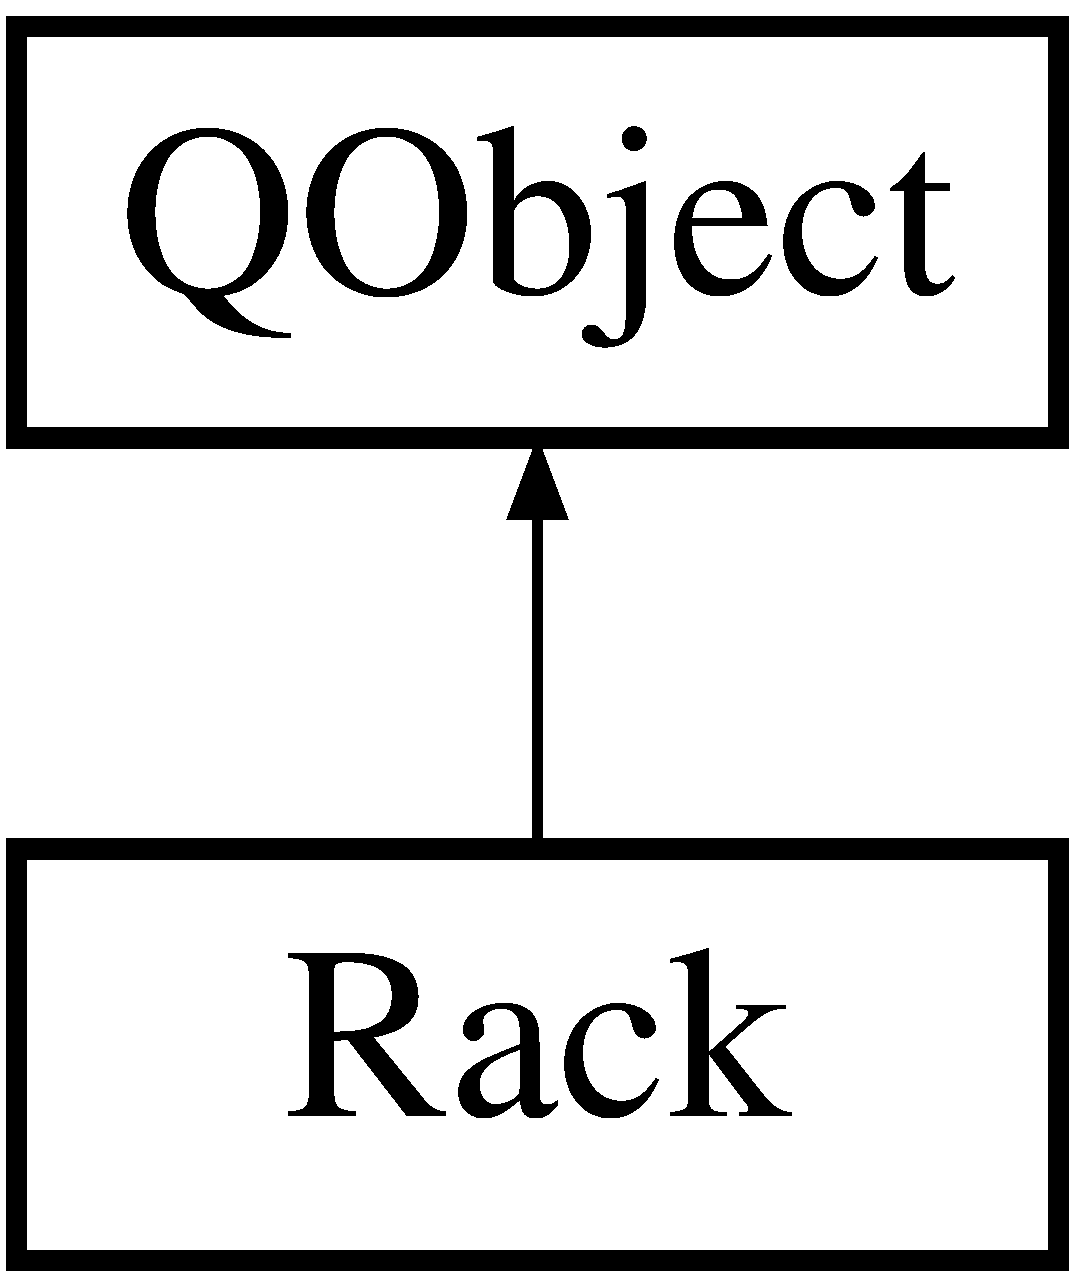
\includegraphics[height=2.000000cm]{class_rack}
\end{center}
\end{figure}
\subsection*{Public Slots}
\begin{DoxyCompactItemize}
\item 
void \hyperlink{class_rack_a7c2b198bbb87eda22a2524781dc09da3}{on\-\_\-cancel\-Button\-\_\-clicked} ()
\begin{DoxyCompactList}\small\item\em \hyperlink{class_rack_a7c2b198bbb87eda22a2524781dc09da3}{Rack\-::on\-\_\-cancel\-Button\-\_\-clicked} Handles the cancel\-Button\-\_\-clicked events. \end{DoxyCompactList}\item 
void \hyperlink{class_rack_a65c2e50299cb5ad7111ad56132b18c29}{on\-\_\-invalid\-Move} ()
\begin{DoxyCompactList}\small\item\em \hyperlink{class_rack_a65c2e50299cb5ad7111ad56132b18c29}{Rack\-::on\-\_\-invalid\-Move} Handles invalide\-Move events. \end{DoxyCompactList}\end{DoxyCompactItemize}
\subsection*{Public Member Functions}
\begin{DoxyCompactItemize}
\item 
\hyperlink{class_rack_aa18464e4a5e7048969a95526c70b3afb}{$\sim$\-Rack} ()
\begin{DoxyCompactList}\small\item\em \hyperlink{class_rack_aa18464e4a5e7048969a95526c70b3afb}{Rack\-::$\sim$\-Rack} Destructor. \end{DoxyCompactList}\item 
\hyperlink{class_rack}{Rack} $\ast$ \hyperlink{class_rack_a3e38244d421dc2b984123b26698028e7}{set\-Space} (int, \hyperlink{class_space}{Space} $\ast$)
\begin{DoxyCompactList}\small\item\em \hyperlink{class_rack_a3e38244d421dc2b984123b26698028e7}{Rack\-::set\-Space} Setter for a space. \end{DoxyCompactList}\item 
\hyperlink{class_space}{Space} $\ast$ \hyperlink{class_rack_a2fdfa2264bb85c08ebf107e67cfc8657}{get\-Space} (int)
\begin{DoxyCompactList}\small\item\em \hyperlink{class_rack_a2fdfa2264bb85c08ebf107e67cfc8657}{Rack\-::get\-Space} Gets the space at an index. \end{DoxyCompactList}\item 
\hyperlink{class_rack}{Rack} $\ast$ \hyperlink{class_rack_ae1b5a6e15cb1ebe299356959b6a8d641}{refresh} (\hyperlink{class_game}{Game} $\ast$)
\begin{DoxyCompactList}\small\item\em \hyperlink{class_rack_ae1b5a6e15cb1ebe299356959b6a8d641}{Rack\-::refresh} Refreshes the rack to show the rack of the current player. \end{DoxyCompactList}\item 
bool \hyperlink{class_rack_a5bd6dd499aecf9239831aafc1679a768}{is\-Active} ()
\begin{DoxyCompactList}\small\item\em \hyperlink{class_rack_a5bd6dd499aecf9239831aafc1679a768}{Rack\-::is\-Active} Is the space active. \end{DoxyCompactList}\item 
void \hyperlink{class_rack_afdf845eb458b07ed6029d29672ab120f}{inactivate\-By\-Letter} (\hyperlink{class_letter}{Letter} $\ast$)
\begin{DoxyCompactList}\small\item\em \hyperlink{class_rack_afdf845eb458b07ed6029d29672ab120f}{Rack\-::inactivate\-By\-Letter} Inactivates a space by the letter is points to. \end{DoxyCompactList}\item 
\hyperlink{class_rack}{Rack} $\ast$ \hyperlink{class_rack_a93f23b989fbb09c0acfb42b24d071887}{delete\-Letter} (\hyperlink{class_letter}{Letter} $\ast$)
\begin{DoxyCompactList}\small\item\em \hyperlink{class_rack_a93f23b989fbb09c0acfb42b24d071887}{Rack\-::delete\-Letter} Deletes a letter from the rack. \end{DoxyCompactList}\item 
\hyperlink{class_rack}{Rack} $\ast$ \hyperlink{class_rack_a66591f08659676ac81eeec7f49f7e1ef}{inactivate\-Other\-Spaces} (int)
\begin{DoxyCompactList}\small\item\em \hyperlink{class_rack_a66591f08659676ac81eeec7f49f7e1ef}{Rack\-::inactivate\-Other\-Spaces} Inactivates other spaces in the rack. \end{DoxyCompactList}\item 
int \hyperlink{class_rack_adcaff679bc9261d773505a0bb132ab96}{get\-Active\-Index} ()
\begin{DoxyCompactList}\small\item\em \hyperlink{class_rack_adcaff679bc9261d773505a0bb132ab96}{Rack\-::get\-Active\-Index} Gets the index of the currently active space. \end{DoxyCompactList}\item 
int \hyperlink{class_rack_aa350328de6aa50d65c63556b930de13b}{get\-Pos} (\hyperlink{class_letter}{Letter} $\ast$L)
\begin{DoxyCompactList}\small\item\em \hyperlink{class_rack_aa350328de6aa50d65c63556b930de13b}{Rack\-::get\-Pos} Gets the position of the \hyperlink{class_rack}{Rack} based on the letter address provided. \end{DoxyCompactList}\end{DoxyCompactItemize}
\subsection*{Static Public Member Functions}
\begin{DoxyCompactItemize}
\item 
static \hyperlink{class_rack}{Rack} $\ast$ \hyperlink{class_rack_aa48de650c15bda8267451d84caf6ea3f}{get\-Rack} ()
\begin{DoxyCompactList}\small\item\em \hyperlink{class_rack_aa48de650c15bda8267451d84caf6ea3f}{Rack\-::get\-Rack} Gets the rack or creates a new one. \end{DoxyCompactList}\end{DoxyCompactItemize}
\subsection*{Private Member Functions}
\begin{DoxyCompactItemize}
\item 
\hyperlink{class_rack_ae14b4c67c853471c6ea8a4813847a98c}{Rack} (Q\-Object $\ast$parent=0)
\begin{DoxyCompactList}\small\item\em \hyperlink{class_rack_ae14b4c67c853471c6ea8a4813847a98c}{Rack\-::\-Rack} Constructor. \end{DoxyCompactList}\end{DoxyCompactItemize}
\subsection*{Private Attributes}
\begin{DoxyCompactItemize}
\item 
\hyperlink{class_space}{Space} $\ast$ \hyperlink{class_rack_a05c2ab5154aed4dde5306f7847ffad4b}{spaces} \mbox{[}\hyperlink{rack_8h_ad52276b6cc76ff4be1f71000a9094f31}{R\-A\-C\-K\-S\-I\-Z\-E}\mbox{]}
\end{DoxyCompactItemize}
\subsection*{Static Private Attributes}
\begin{DoxyCompactItemize}
\item 
static bool \hyperlink{class_rack_afcffaefc94d794ec29c52b5899f1d55f}{is\-Set} = false
\item 
static \hyperlink{class_rack}{Rack} $\ast$ \hyperlink{class_rack_afac5cd813452f1191075fcbc4413ffb3}{rack} = N\-U\-L\-L
\end{DoxyCompactItemize}


\subsection{Detailed Description}
The \hyperlink{class_rack}{Rack} class Singleton class representing the current player on the \hyperlink{class_dialog}{Dialog}. 

Definition at line 16 of file rack.\-h.



\subsection{Constructor \& Destructor Documentation}
\hypertarget{class_rack_aa18464e4a5e7048969a95526c70b3afb}{\index{Rack@{Rack}!$\sim$\-Rack@{$\sim$\-Rack}}
\index{$\sim$\-Rack@{$\sim$\-Rack}!Rack@{Rack}}
\subsubsection[{$\sim$\-Rack}]{\setlength{\rightskip}{0pt plus 5cm}Rack\-::$\sim$\-Rack (
\begin{DoxyParamCaption}
{}
\end{DoxyParamCaption}
)}}\label{class_rack_aa18464e4a5e7048969a95526c70b3afb}


\hyperlink{class_rack_aa18464e4a5e7048969a95526c70b3afb}{Rack\-::$\sim$\-Rack} Destructor. 



Definition at line 35 of file rack.\-cpp.



References R\-A\-C\-K\-S\-I\-Z\-E, and spaces.


\begin{DoxyCode}
36 \{
37     \textcolor{keywordflow}{for} (\textcolor{keywordtype}{int} i = 0; i < \hyperlink{rack_8h_ad52276b6cc76ff4be1f71000a9094f31}{RACKSIZE}; i++)\{
38         \textcolor{keyword}{delete}(\hyperlink{class_rack_a05c2ab5154aed4dde5306f7847ffad4b}{spaces}[i]);
39     \}
40 \}
\end{DoxyCode}
\hypertarget{class_rack_ae14b4c67c853471c6ea8a4813847a98c}{\index{Rack@{Rack}!Rack@{Rack}}
\index{Rack@{Rack}!Rack@{Rack}}
\subsubsection[{Rack}]{\setlength{\rightskip}{0pt plus 5cm}Rack\-::\-Rack (
\begin{DoxyParamCaption}
\item[{Q\-Object $\ast$}]{parent = {\ttfamily 0}}
\end{DoxyParamCaption}
)\hspace{0.3cm}{\ttfamily [explicit]}, {\ttfamily [private]}}}\label{class_rack_ae14b4c67c853471c6ea8a4813847a98c}


\hyperlink{class_rack_ae14b4c67c853471c6ea8a4813847a98c}{Rack\-::\-Rack} Constructor. 


\begin{DoxyParams}{Parameters}
{\em parent} & The parent \\
\hline
\end{DoxyParams}


Definition at line 10 of file rack.\-cpp.



References R\-A\-C\-K\-S\-I\-Z\-E, and spaces.



Referenced by get\-Rack().


\begin{DoxyCode}
10                           :
11     QObject(parent)
12 \{
13     \textcolor{keywordflow}{for} (\textcolor{keywordtype}{int} i = 0; i < \hyperlink{rack_8h_ad52276b6cc76ff4be1f71000a9094f31}{RACKSIZE}; i++)\{
14         \hyperlink{class_rack_a05c2ab5154aed4dde5306f7847ffad4b}{spaces}[i] = \textcolor{keyword}{new} \hyperlink{class_space}{Space}(i);
15     \}
16 \}
\end{DoxyCode}


\subsection{Member Function Documentation}
\hypertarget{class_rack_a93f23b989fbb09c0acfb42b24d071887}{\index{Rack@{Rack}!delete\-Letter@{delete\-Letter}}
\index{delete\-Letter@{delete\-Letter}!Rack@{Rack}}
\subsubsection[{delete\-Letter}]{\setlength{\rightskip}{0pt plus 5cm}{\bf Rack} $\ast$ Rack\-::delete\-Letter (
\begin{DoxyParamCaption}
\item[{{\bf Letter} $\ast$}]{letter}
\end{DoxyParamCaption}
)}}\label{class_rack_a93f23b989fbb09c0acfb42b24d071887}


\hyperlink{class_rack_a93f23b989fbb09c0acfb42b24d071887}{Rack\-::delete\-Letter} Deletes a letter from the rack. 


\begin{DoxyParams}{Parameters}
{\em letter} & The letter to conpare to the rack \\
\hline
\end{DoxyParams}
\begin{DoxyReturn}{Returns}
this 
\end{DoxyReturn}


Definition at line 157 of file rack.\-cpp.



References Space\-::clear(), R\-A\-C\-K\-S\-I\-Z\-E, and spaces.



Referenced by Board\-::$\sim$\-Board().


\begin{DoxyCode}
158 \{
159     \textcolor{keywordflow}{for} (\textcolor{keywordtype}{int} i = 0; i < \hyperlink{rack_8h_ad52276b6cc76ff4be1f71000a9094f31}{RACKSIZE}; i++)\{
160         \textcolor{keywordflow}{if} (\hyperlink{class_rack_a05c2ab5154aed4dde5306f7847ffad4b}{spaces}[i]->getLetter() == letter)\{
161             \hyperlink{class_rack_a05c2ab5154aed4dde5306f7847ffad4b}{spaces}[i]->\hyperlink{class_space_ab18791c1da302a91c51477108be478b5}{clear}();
162         \}
163     \}
164     \textcolor{keywordflow}{return} \textcolor{keyword}{this};
165 \}
\end{DoxyCode}
\hypertarget{class_rack_adcaff679bc9261d773505a0bb132ab96}{\index{Rack@{Rack}!get\-Active\-Index@{get\-Active\-Index}}
\index{get\-Active\-Index@{get\-Active\-Index}!Rack@{Rack}}
\subsubsection[{get\-Active\-Index}]{\setlength{\rightskip}{0pt plus 5cm}int Rack\-::get\-Active\-Index (
\begin{DoxyParamCaption}
{}
\end{DoxyParamCaption}
)}}\label{class_rack_adcaff679bc9261d773505a0bb132ab96}


\hyperlink{class_rack_adcaff679bc9261d773505a0bb132ab96}{Rack\-::get\-Active\-Index} Gets the index of the currently active space. 

\begin{DoxyReturn}{Returns}
the index 
\end{DoxyReturn}


Definition at line 118 of file rack.\-cpp.



References is\-Active(), R\-A\-C\-K\-S\-I\-Z\-E, and spaces.


\begin{DoxyCode}
119 \{
120     \textcolor{keywordflow}{for}(\textcolor{keywordtype}{int} i = 0; i < \hyperlink{rack_8h_ad52276b6cc76ff4be1f71000a9094f31}{RACKSIZE}; i++)\{
121         \textcolor{keywordflow}{if} (\hyperlink{class_rack_a05c2ab5154aed4dde5306f7847ffad4b}{spaces}[i]->\hyperlink{class_rack_a5bd6dd499aecf9239831aafc1679a768}{isActive}())\{
122             \textcolor{keywordflow}{return} i;
123         \}
124     \}
125     \textcolor{keywordflow}{return} -1;
126 \}
\end{DoxyCode}
\hypertarget{class_rack_aa350328de6aa50d65c63556b930de13b}{\index{Rack@{Rack}!get\-Pos@{get\-Pos}}
\index{get\-Pos@{get\-Pos}!Rack@{Rack}}
\subsubsection[{get\-Pos}]{\setlength{\rightskip}{0pt plus 5cm}int Rack\-::get\-Pos (
\begin{DoxyParamCaption}
\item[{{\bf Letter} $\ast$}]{L}
\end{DoxyParamCaption}
)}}\label{class_rack_aa350328de6aa50d65c63556b930de13b}


\hyperlink{class_rack_aa350328de6aa50d65c63556b930de13b}{Rack\-::get\-Pos} Gets the position of the \hyperlink{class_rack}{Rack} based on the letter address provided. 


\begin{DoxyParams}{Parameters}
{\em L} & The letter. \\
\hline
\end{DoxyParams}
\begin{DoxyReturn}{Returns}
the integer position on the rack. -\/1 if it doesn't exist. 
\end{DoxyReturn}


Definition at line 143 of file rack.\-cpp.



References spaces.


\begin{DoxyCode}
144 \{
145     \textcolor{keywordflow}{for}(\textcolor{keywordtype}{int} i = 0; i < 7; i++)
146         \textcolor{keywordflow}{if}(this->\hyperlink{class_rack_a05c2ab5154aed4dde5306f7847ffad4b}{spaces}[i]->getLetter() == L)
147             \textcolor{keywordflow}{return} i;
148     \textcolor{keywordflow}{return} -1;
149 \}
\end{DoxyCode}
\hypertarget{class_rack_aa48de650c15bda8267451d84caf6ea3f}{\index{Rack@{Rack}!get\-Rack@{get\-Rack}}
\index{get\-Rack@{get\-Rack}!Rack@{Rack}}
\subsubsection[{get\-Rack}]{\setlength{\rightskip}{0pt plus 5cm}{\bf Rack} $\ast$ Rack\-::get\-Rack (
\begin{DoxyParamCaption}
{}
\end{DoxyParamCaption}
)\hspace{0.3cm}{\ttfamily [static]}}}\label{class_rack_aa48de650c15bda8267451d84caf6ea3f}


\hyperlink{class_rack_aa48de650c15bda8267451d84caf6ea3f}{Rack\-::get\-Rack} Gets the rack or creates a new one. 

\begin{DoxyReturn}{Returns}
The rack 
\end{DoxyReturn}


Definition at line 22 of file rack.\-cpp.



References is\-Set, rack, and Rack().



Referenced by A\-I\-Player\-::\-\_\-assist\-\_\-ai\-\_\-search(), Move\-::apply(), Dialog\-::create\-Horizontal\-Group\-Box(), Dialog\-::\-Dialog(), Player\-::get\-New\-Letters(), Board\-::move\-Letter\-To\-Board(), Game\-::next\-Turn(), Space\-::on\-\_\-clicked(), A\-I\-Player\-::play(), Move\-::unapply(), and Board\-::$\sim$\-Board().


\begin{DoxyCode}
23 \{
24     \textcolor{keywordflow}{if}(\hyperlink{class_rack_afcffaefc94d794ec29c52b5899f1d55f}{isSet})\{
25         \textcolor{keywordflow}{return} \hyperlink{class_rack_afac5cd813452f1191075fcbc4413ffb3}{rack};
26     \}
27     \hyperlink{class_rack_afcffaefc94d794ec29c52b5899f1d55f}{isSet} = \textcolor{keyword}{true};
28     \hyperlink{class_rack_afac5cd813452f1191075fcbc4413ffb3}{rack} = \textcolor{keyword}{new} \hyperlink{class_rack_ae14b4c67c853471c6ea8a4813847a98c}{Rack}();
29     \textcolor{keywordflow}{return} \hyperlink{class_rack_afac5cd813452f1191075fcbc4413ffb3}{rack};
30 \}
\end{DoxyCode}
\hypertarget{class_rack_a2fdfa2264bb85c08ebf107e67cfc8657}{\index{Rack@{Rack}!get\-Space@{get\-Space}}
\index{get\-Space@{get\-Space}!Rack@{Rack}}
\subsubsection[{get\-Space}]{\setlength{\rightskip}{0pt plus 5cm}{\bf Space} $\ast$ Rack\-::get\-Space (
\begin{DoxyParamCaption}
\item[{int}]{i}
\end{DoxyParamCaption}
)}}\label{class_rack_a2fdfa2264bb85c08ebf107e67cfc8657}


\hyperlink{class_rack_a2fdfa2264bb85c08ebf107e67cfc8657}{Rack\-::get\-Space} Gets the space at an index. 


\begin{DoxyParams}{Parameters}
{\em i} & The index \\
\hline
\end{DoxyParams}
\begin{DoxyReturn}{Returns}
The space at i 
\end{DoxyReturn}


Definition at line 133 of file rack.\-cpp.



References spaces.



Referenced by Move\-::apply(), Dialog\-::create\-Horizontal\-Group\-Box(), and Move\-::unapply().


\begin{DoxyCode}
134 \{
135     \textcolor{keywordflow}{return} \hyperlink{class_rack_a05c2ab5154aed4dde5306f7847ffad4b}{spaces}[i];
136 \}
\end{DoxyCode}
\hypertarget{class_rack_afdf845eb458b07ed6029d29672ab120f}{\index{Rack@{Rack}!inactivate\-By\-Letter@{inactivate\-By\-Letter}}
\index{inactivate\-By\-Letter@{inactivate\-By\-Letter}!Rack@{Rack}}
\subsubsection[{inactivate\-By\-Letter}]{\setlength{\rightskip}{0pt plus 5cm}void Rack\-::inactivate\-By\-Letter (
\begin{DoxyParamCaption}
\item[{{\bf Letter} $\ast$}]{letter}
\end{DoxyParamCaption}
)}}\label{class_rack_afdf845eb458b07ed6029d29672ab120f}


\hyperlink{class_rack_afdf845eb458b07ed6029d29672ab120f}{Rack\-::inactivate\-By\-Letter} Inactivates a space by the letter is points to. 


\begin{DoxyParams}{Parameters}
{\em letter} & The letter used to compare \\
\hline
\end{DoxyParams}


Definition at line 75 of file rack.\-cpp.



References R\-A\-C\-K\-S\-I\-Z\-E, Space\-::set\-Inactive(), and spaces.



Referenced by Space\-::on\-\_\-clicked(), and A\-I\-Player\-::play().


\begin{DoxyCode}
76 \{
77     \textcolor{keywordflow}{for} (\textcolor{keywordtype}{int} i = 0; i < \hyperlink{rack_8h_ad52276b6cc76ff4be1f71000a9094f31}{RACKSIZE}; i++)\{
78         \textcolor{keywordflow}{if} (\hyperlink{class_rack_a05c2ab5154aed4dde5306f7847ffad4b}{spaces}[i]->getLetter() == letter)\{
79             \hyperlink{class_rack_a05c2ab5154aed4dde5306f7847ffad4b}{spaces}[i]->\hyperlink{class_space_a8f6b89f570c1e0ca3c34f19df439a598}{setInactive}();
80         \}
81     \}
82 \}
\end{DoxyCode}
\hypertarget{class_rack_a66591f08659676ac81eeec7f49f7e1ef}{\index{Rack@{Rack}!inactivate\-Other\-Spaces@{inactivate\-Other\-Spaces}}
\index{inactivate\-Other\-Spaces@{inactivate\-Other\-Spaces}!Rack@{Rack}}
\subsubsection[{inactivate\-Other\-Spaces}]{\setlength{\rightskip}{0pt plus 5cm}{\bf Rack} $\ast$ Rack\-::inactivate\-Other\-Spaces (
\begin{DoxyParamCaption}
\item[{int}]{x}
\end{DoxyParamCaption}
)}}\label{class_rack_a66591f08659676ac81eeec7f49f7e1ef}


\hyperlink{class_rack_a66591f08659676ac81eeec7f49f7e1ef}{Rack\-::inactivate\-Other\-Spaces} Inactivates other spaces in the rack. 


\begin{DoxyParams}{Parameters}
{\em x} & The position not to inactivate \\
\hline
\end{DoxyParams}
\begin{DoxyReturn}{Returns}
this 
\end{DoxyReturn}


Definition at line 60 of file rack.\-cpp.



References is\-Active(), R\-A\-C\-K\-S\-I\-Z\-E, Space\-::set\-Inactive(), and spaces.



Referenced by Space\-::on\-\_\-clicked().


\begin{DoxyCode}
61 \{
62     \textcolor{keywordflow}{for} (\textcolor{keywordtype}{int} i = 0; i < \hyperlink{rack_8h_ad52276b6cc76ff4be1f71000a9094f31}{RACKSIZE}; i++)\{
63         \textcolor{keywordflow}{if} (x != i && \hyperlink{class_rack_a05c2ab5154aed4dde5306f7847ffad4b}{spaces}[i]->\hyperlink{class_rack_a5bd6dd499aecf9239831aafc1679a768}{isActive}())\{
64             \hyperlink{class_rack_a05c2ab5154aed4dde5306f7847ffad4b}{spaces}[i]->\hyperlink{class_space_a8f6b89f570c1e0ca3c34f19df439a598}{setInactive}();
65         \}
66     \}
67     \textcolor{keywordflow}{return} \textcolor{keyword}{this};
68 \}
\end{DoxyCode}
\hypertarget{class_rack_a5bd6dd499aecf9239831aafc1679a768}{\index{Rack@{Rack}!is\-Active@{is\-Active}}
\index{is\-Active@{is\-Active}!Rack@{Rack}}
\subsubsection[{is\-Active}]{\setlength{\rightskip}{0pt plus 5cm}bool Rack\-::is\-Active (
\begin{DoxyParamCaption}
{}
\end{DoxyParamCaption}
)}}\label{class_rack_a5bd6dd499aecf9239831aafc1679a768}


\hyperlink{class_rack_a5bd6dd499aecf9239831aafc1679a768}{Rack\-::is\-Active} Is the space active. 

\begin{DoxyReturn}{Returns}
true if active 
\end{DoxyReturn}


Definition at line 103 of file rack.\-cpp.



References R\-A\-C\-K\-S\-I\-Z\-E, and spaces.



Referenced by get\-Active\-Index(), and inactivate\-Other\-Spaces().


\begin{DoxyCode}
104 \{
105     \textcolor{keywordflow}{for}(\textcolor{keywordtype}{int} i = 0; i < \hyperlink{rack_8h_ad52276b6cc76ff4be1f71000a9094f31}{RACKSIZE}; i++)\{
106         \textcolor{keywordflow}{if} (\hyperlink{class_rack_a05c2ab5154aed4dde5306f7847ffad4b}{spaces}[i]->\hyperlink{class_rack_a5bd6dd499aecf9239831aafc1679a768}{isActive}())\{
107             \textcolor{keywordflow}{return} \textcolor{keyword}{true};
108         \}
109     \}
110     \textcolor{keywordflow}{return} \textcolor{keyword}{false};
111 \}
\end{DoxyCode}
\hypertarget{class_rack_a7c2b198bbb87eda22a2524781dc09da3}{\index{Rack@{Rack}!on\-\_\-cancel\-Button\-\_\-clicked@{on\-\_\-cancel\-Button\-\_\-clicked}}
\index{on\-\_\-cancel\-Button\-\_\-clicked@{on\-\_\-cancel\-Button\-\_\-clicked}!Rack@{Rack}}
\subsubsection[{on\-\_\-cancel\-Button\-\_\-clicked}]{\setlength{\rightskip}{0pt plus 5cm}void Rack\-::on\-\_\-cancel\-Button\-\_\-clicked (
\begin{DoxyParamCaption}
{}
\end{DoxyParamCaption}
)\hspace{0.3cm}{\ttfamily [slot]}}}\label{class_rack_a7c2b198bbb87eda22a2524781dc09da3}


\hyperlink{class_rack_a7c2b198bbb87eda22a2524781dc09da3}{Rack\-::on\-\_\-cancel\-Button\-\_\-clicked} Handles the cancel\-Button\-\_\-clicked events. 



Definition at line 171 of file rack.\-cpp.



References R\-A\-C\-K\-S\-I\-Z\-E, Space\-::set\-Inactive(), and spaces.


\begin{DoxyCode}
172 \{
173     \textcolor{keywordflow}{for} (\textcolor{keywordtype}{int} i = 0; i < \hyperlink{rack_8h_ad52276b6cc76ff4be1f71000a9094f31}{RACKSIZE}; i++)\{
174         \textcolor{keywordflow}{if} (\hyperlink{class_rack_a05c2ab5154aed4dde5306f7847ffad4b}{spaces}[i]->isPlaced()) \{
175             \hyperlink{class_rack_a05c2ab5154aed4dde5306f7847ffad4b}{spaces}[i]->\hyperlink{class_space_a8f6b89f570c1e0ca3c34f19df439a598}{setInactive}();
176         \}
177     \}
178 \}
\end{DoxyCode}
\hypertarget{class_rack_a65c2e50299cb5ad7111ad56132b18c29}{\index{Rack@{Rack}!on\-\_\-invalid\-Move@{on\-\_\-invalid\-Move}}
\index{on\-\_\-invalid\-Move@{on\-\_\-invalid\-Move}!Rack@{Rack}}
\subsubsection[{on\-\_\-invalid\-Move}]{\setlength{\rightskip}{0pt plus 5cm}void Rack\-::on\-\_\-invalid\-Move (
\begin{DoxyParamCaption}
{}
\end{DoxyParamCaption}
)\hspace{0.3cm}{\ttfamily [slot]}}}\label{class_rack_a65c2e50299cb5ad7111ad56132b18c29}


\hyperlink{class_rack_a65c2e50299cb5ad7111ad56132b18c29}{Rack\-::on\-\_\-invalid\-Move} Handles invalide\-Move events. 



Definition at line 183 of file rack.\-cpp.



References R\-A\-C\-K\-S\-I\-Z\-E, Space\-::set\-Inactive(), and spaces.


\begin{DoxyCode}
184 \{
185     \textcolor{keywordflow}{for} (\textcolor{keywordtype}{int} i = 0; i < \hyperlink{rack_8h_ad52276b6cc76ff4be1f71000a9094f31}{RACKSIZE}; i++)\{
186         \textcolor{keywordflow}{if} (\hyperlink{class_rack_a05c2ab5154aed4dde5306f7847ffad4b}{spaces}[i]->isPlaced()) \{
187             \hyperlink{class_rack_a05c2ab5154aed4dde5306f7847ffad4b}{spaces}[i]->\hyperlink{class_space_a8f6b89f570c1e0ca3c34f19df439a598}{setInactive}();
188         \}
189     \}
190 \}
\end{DoxyCode}
\hypertarget{class_rack_ae1b5a6e15cb1ebe299356959b6a8d641}{\index{Rack@{Rack}!refresh@{refresh}}
\index{refresh@{refresh}!Rack@{Rack}}
\subsubsection[{refresh}]{\setlength{\rightskip}{0pt plus 5cm}{\bf Rack} $\ast$ Rack\-::refresh (
\begin{DoxyParamCaption}
\item[{{\bf Game} $\ast$}]{game}
\end{DoxyParamCaption}
)}}\label{class_rack_ae1b5a6e15cb1ebe299356959b6a8d641}


\hyperlink{class_rack_ae1b5a6e15cb1ebe299356959b6a8d641}{Rack\-::refresh} Refreshes the rack to show the rack of the current player. 


\begin{DoxyParams}{Parameters}
{\em game} & The game \\
\hline
\end{DoxyParams}
\begin{DoxyReturn}{Returns}
this 
\end{DoxyReturn}


Definition at line 90 of file rack.\-cpp.



References Space\-::clear(), Game\-::current\-Player(), Player\-::get\-Letter(), R\-A\-C\-K\-S\-I\-Z\-E, Space\-::set\-Letter(), and spaces.



Referenced by Game\-::next\-Turn(), and Dialog\-::setup\-Game().


\begin{DoxyCode}
91 \{
92     \textcolor{keywordflow}{for} (\textcolor{keywordtype}{int} i = 0; i < \hyperlink{rack_8h_ad52276b6cc76ff4be1f71000a9094f31}{RACKSIZE}; i++)\{
93         \hyperlink{class_rack_a05c2ab5154aed4dde5306f7847ffad4b}{spaces}[i]->\hyperlink{class_space_ab18791c1da302a91c51477108be478b5}{clear}();
94         \hyperlink{class_rack_a05c2ab5154aed4dde5306f7847ffad4b}{spaces}[i]->\hyperlink{class_space_aab86690461768d190a009e06c753f2ce}{setLetter}(game->\hyperlink{class_game_a7cdf3f086fafd3234dba20409e9b98d3}{currentPlayer}()->
      \hyperlink{class_player_aa6aabfbae536fec650fd466f65fb9743}{getLetter}(i));
95     \}
96     \textcolor{keywordflow}{return} \textcolor{keyword}{this};
97 \}
\end{DoxyCode}
\hypertarget{class_rack_a3e38244d421dc2b984123b26698028e7}{\index{Rack@{Rack}!set\-Space@{set\-Space}}
\index{set\-Space@{set\-Space}!Rack@{Rack}}
\subsubsection[{set\-Space}]{\setlength{\rightskip}{0pt plus 5cm}{\bf Rack} $\ast$ Rack\-::set\-Space (
\begin{DoxyParamCaption}
\item[{int}]{i, }
\item[{{\bf Space} $\ast$}]{space}
\end{DoxyParamCaption}
)}}\label{class_rack_a3e38244d421dc2b984123b26698028e7}


\hyperlink{class_rack_a3e38244d421dc2b984123b26698028e7}{Rack\-::set\-Space} Setter for a space. 


\begin{DoxyParams}{Parameters}
{\em i} & The position to set \\
\hline
{\em space} & The space to set \\
\hline
\end{DoxyParams}
\begin{DoxyReturn}{Returns}
this 
\end{DoxyReturn}


Definition at line 48 of file rack.\-cpp.



References spaces.


\begin{DoxyCode}
49 \{
50     \hyperlink{class_rack_a05c2ab5154aed4dde5306f7847ffad4b}{spaces}[i] = space;
51     \textcolor{keywordflow}{return} \textcolor{keyword}{this};
52 \}
\end{DoxyCode}


\subsection{Member Data Documentation}
\hypertarget{class_rack_afcffaefc94d794ec29c52b5899f1d55f}{\index{Rack@{Rack}!is\-Set@{is\-Set}}
\index{is\-Set@{is\-Set}!Rack@{Rack}}
\subsubsection[{is\-Set}]{\setlength{\rightskip}{0pt plus 5cm}bool Rack\-::is\-Set = false\hspace{0.3cm}{\ttfamily [static]}, {\ttfamily [private]}}}\label{class_rack_afcffaefc94d794ec29c52b5899f1d55f}
Flag if the \hyperlink{class_rack}{Rack} has been set 

Definition at line 35 of file rack.\-h.



Referenced by get\-Rack().

\hypertarget{class_rack_afac5cd813452f1191075fcbc4413ffb3}{\index{Rack@{Rack}!rack@{rack}}
\index{rack@{rack}!Rack@{Rack}}
\subsubsection[{rack}]{\setlength{\rightskip}{0pt plus 5cm}{\bf Rack} $\ast$ Rack\-::rack = N\-U\-L\-L\hspace{0.3cm}{\ttfamily [static]}, {\ttfamily [private]}}}\label{class_rack_afac5cd813452f1191075fcbc4413ffb3}
The \hyperlink{class_rack}{Rack} 

Definition at line 36 of file rack.\-h.



Referenced by get\-Rack().

\hypertarget{class_rack_a05c2ab5154aed4dde5306f7847ffad4b}{\index{Rack@{Rack}!spaces@{spaces}}
\index{spaces@{spaces}!Rack@{Rack}}
\subsubsection[{spaces}]{\setlength{\rightskip}{0pt plus 5cm}{\bf Space}$\ast$ Rack\-::spaces\mbox{[}{\bf R\-A\-C\-K\-S\-I\-Z\-E}\mbox{]}\hspace{0.3cm}{\ttfamily [private]}}}\label{class_rack_a05c2ab5154aed4dde5306f7847ffad4b}
The container for the Spaces 

Definition at line 37 of file rack.\-h.



Referenced by delete\-Letter(), get\-Active\-Index(), get\-Pos(), get\-Space(), inactivate\-By\-Letter(), inactivate\-Other\-Spaces(), is\-Active(), on\-\_\-cancel\-Button\-\_\-clicked(), on\-\_\-invalid\-Move(), Rack(), refresh(), set\-Space(), and $\sim$\-Rack().



The documentation for this class was generated from the following files\-:\begin{DoxyCompactItemize}
\item 
Scrabble/\hyperlink{rack_8h}{rack.\-h}\item 
Scrabble/\hyperlink{rack_8cpp}{rack.\-cpp}\end{DoxyCompactItemize}

\hypertarget{class_space}{\section{Space Class Reference}
\label{class_space}\index{Space@{Space}}
}


The \hyperlink{class_space}{Space} class A visual representation of a space on the board that may or may not be filled with a \hyperlink{class_letter}{Letter}.  




{\ttfamily \#include $<$space.\-h$>$}

Inheritance diagram for Space\-:\begin{figure}[H]
\begin{center}
\leavevmode
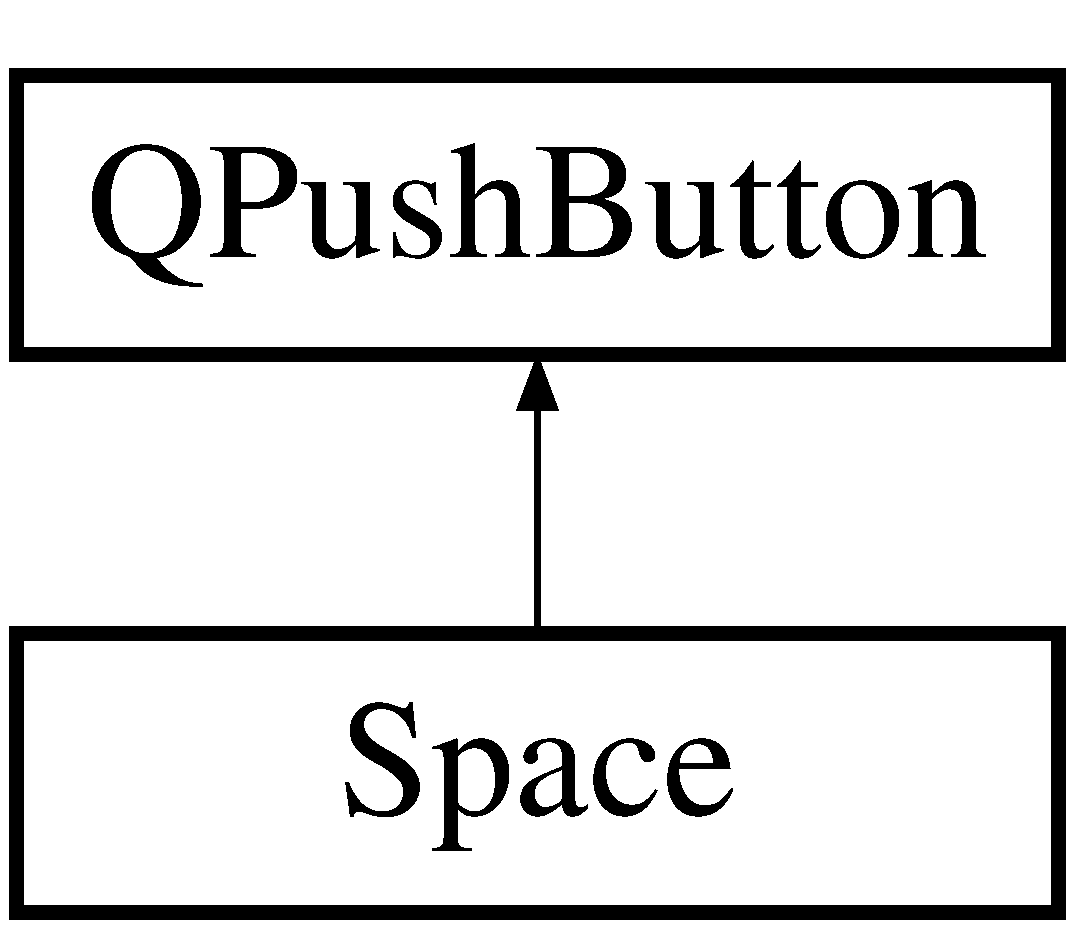
\includegraphics[height=2.000000cm]{class_space}
\end{center}
\end{figure}
\subsection*{Public Slots}
\begin{DoxyCompactItemize}
\item 
void \hyperlink{class_space_a762303973d71621706a7a8195bd0f946}{on\-\_\-clicked} ()
\begin{DoxyCompactList}\small\item\em \hyperlink{class_space_a762303973d71621706a7a8195bd0f946}{Space\-::on\-\_\-clicked} Handles on\-\_\-cicked events. \end{DoxyCompactList}\end{DoxyCompactItemize}
\subsection*{Public Member Functions}
\begin{DoxyCompactItemize}
\item 
\hyperlink{class_space_a215e62ed852d6f6ba3de07d91c9ff236}{Space} (int, int, int, int, Q\-String, Q\-String)
\begin{DoxyCompactList}\small\item\em \hyperlink{class_space_a215e62ed852d6f6ba3de07d91c9ff236}{Space\-::\-Space} Constructor. \end{DoxyCompactList}\item 
\hyperlink{class_space_a7ccd72aff73f5e5c274790009cdbaf37}{Space} (int)
\begin{DoxyCompactList}\small\item\em \hyperlink{class_space_a215e62ed852d6f6ba3de07d91c9ff236}{Space\-::\-Space} Default constructor for space object. \end{DoxyCompactList}\item 
\hyperlink{class_space_a06d440a35bcb4b1554b69e8b18d53705}{$\sim$\-Space} ()
\begin{DoxyCompactList}\small\item\em \hyperlink{class_space_a06d440a35bcb4b1554b69e8b18d53705}{Space\-::$\sim$\-Space} Destructor. \end{DoxyCompactList}\item 
\hyperlink{class_space_adb7de4055fa9c105d8f62f83660806ce}{Space} (const \hyperlink{class_space}{Space} \&other)
\begin{DoxyCompactList}\small\item\em \hyperlink{class_space_a215e62ed852d6f6ba3de07d91c9ff236}{Space\-::\-Space} Copy constructor. \end{DoxyCompactList}\item 
\hyperlink{class_space}{Space} $\ast$ \hyperlink{class_space_aab86690461768d190a009e06c753f2ce}{set\-Letter} (\hyperlink{class_letter}{Letter} $\ast$)
\begin{DoxyCompactList}\small\item\em \hyperlink{class_space_aab86690461768d190a009e06c753f2ce}{Space\-::set\-Letter} Setter for letter. \end{DoxyCompactList}\item 
\hyperlink{class_space}{Space} $\ast$ \hyperlink{class_space_a504f4eb0ec7193df72b161745aa8086e}{set\-Start\-Space} (bool)
\begin{DoxyCompactList}\small\item\em \hyperlink{class_space_a504f4eb0ec7193df72b161745aa8086e}{Space\-::set\-Start\-Space} Sets a starting space. \end{DoxyCompactList}\item 
\hyperlink{class_space}{Space} $\ast$ \hyperlink{class_space_ab18791c1da302a91c51477108be478b5}{clear} ()
\begin{DoxyCompactList}\small\item\em Space\-::clear\-Letter Clears the letter. \end{DoxyCompactList}\item 
\hyperlink{class_space}{Space} $\ast$ \hyperlink{class_space_a999461c4a81ac0028c5780e5c0f2aebf}{set\-Color} (Q\-String \hyperlink{class_space_aa26e0bcc52344b863a274af75651e454}{color})
\begin{DoxyCompactList}\small\item\em \hyperlink{class_space_a999461c4a81ac0028c5780e5c0f2aebf}{Space\-::set\-Color} Sets the color. \end{DoxyCompactList}\item 
\hyperlink{class_letter}{Letter} $\ast$ \hyperlink{class_space_a207bc025538775ce43bdcc0d8c4c3599}{get\-Letter} ()
\begin{DoxyCompactList}\small\item\em \hyperlink{class_space_a207bc025538775ce43bdcc0d8c4c3599}{Space\-::get\-Letter} Getter for letter. \end{DoxyCompactList}\item 
Q\-String \hyperlink{class_space_a32d88c2b9a0f1671ed3ebbd51ec9db09}{get\-Color} ()
\begin{DoxyCompactList}\small\item\em \hyperlink{class_space_a32d88c2b9a0f1671ed3ebbd51ec9db09}{Space\-::get\-Color} Getter for color. \end{DoxyCompactList}\item 
int \hyperlink{class_space_a9d17383ff1ff7ef3dd0be617ad69436c}{get\-Value} ()
\begin{DoxyCompactList}\small\item\em \hyperlink{class_space_a9d17383ff1ff7ef3dd0be617ad69436c}{Space\-::get\-Value} Get the value of the space. \end{DoxyCompactList}\item 
int \hyperlink{class_space_af35759deb33db2b7b7c77a40716c179f}{get\-Letter\-Multiplier} ()
\begin{DoxyCompactList}\small\item\em \hyperlink{class_space_af35759deb33db2b7b7c77a40716c179f}{Space\-::get\-Letter\-Multiplier} Getter for letter multiplier. \end{DoxyCompactList}\item 
int \hyperlink{class_space_a6a26a281a90288d56c83cc76b53cb6fb}{get\-Word\-Multiplier} ()
\begin{DoxyCompactList}\small\item\em \hyperlink{class_space_a6a26a281a90288d56c83cc76b53cb6fb}{Space\-::get\-Word\-Multiplier} Getter for word multiplier. \end{DoxyCompactList}\item 
int \hyperlink{class_space_a65828dd5c8d2799dadab676c1d52bdfa}{get\-X} ()
\begin{DoxyCompactList}\small\item\em \hyperlink{class_space_a65828dd5c8d2799dadab676c1d52bdfa}{Space\-::get\-X} Getter for x. \end{DoxyCompactList}\item 
int \hyperlink{class_space_ac12e951586a96323b1db8cf1e5a827a9}{get\-Y} ()
\begin{DoxyCompactList}\small\item\em \hyperlink{class_space_ac12e951586a96323b1db8cf1e5a827a9}{Space\-::get\-Y} Getter for y. \end{DoxyCompactList}\item 
bool \hyperlink{class_space_aaa6f84cc3a3877b7fb32e5b2363adb10}{is\-Start\-Space} ()
\begin{DoxyCompactList}\small\item\em \hyperlink{class_space_aaa6f84cc3a3877b7fb32e5b2363adb10}{Space\-::is\-Start\-Space} Is the space the start space. \end{DoxyCompactList}\item 
bool \hyperlink{class_space_a83819948ab0508299c66829ca8335034}{is\-Inactive} ()
\begin{DoxyCompactList}\small\item\em \hyperlink{class_space_a83819948ab0508299c66829ca8335034}{Space\-::is\-Inactive} Is the space inactive. \end{DoxyCompactList}\item 
bool \hyperlink{class_space_a7aec01e1b32d70af2cdc25d298517d6c}{is\-Active} ()
\begin{DoxyCompactList}\small\item\em \hyperlink{class_space_a7aec01e1b32d70af2cdc25d298517d6c}{Space\-::is\-Active} Is the space active. \end{DoxyCompactList}\item 
bool \hyperlink{class_space_aa24aa1c8ac8b6033fc041d79345bac71}{is\-New} ()
\begin{DoxyCompactList}\small\item\em \hyperlink{class_space_aa24aa1c8ac8b6033fc041d79345bac71}{Space\-::is\-New} Is the space new. \end{DoxyCompactList}\item 
bool \hyperlink{class_space_a6aa96af44b69e725c4891ad83be05dbd}{is\-Placed} ()
\begin{DoxyCompactList}\small\item\em \hyperlink{class_space_a6aa96af44b69e725c4891ad83be05dbd}{Space\-::is\-Placed} Is the space placed. \end{DoxyCompactList}\item 
bool \hyperlink{class_space_a308f0ef400183df78df69717ca50cfee}{is\-Blank} ()
\begin{DoxyCompactList}\small\item\em \hyperlink{class_space_a308f0ef400183df78df69717ca50cfee}{Space\-::is\-Blank} Is the space blank. \end{DoxyCompactList}\item 
bool \hyperlink{class_space_a5af5885e0b62f4d13ed32c86e50f3cfe}{is\-On\-Board} ()
\begin{DoxyCompactList}\small\item\em \hyperlink{class_space_a5af5885e0b62f4d13ed32c86e50f3cfe}{Space\-::is\-On\-Board} Is the space on the board. \end{DoxyCompactList}\item 
\hyperlink{class_space}{Space} $\ast$ \hyperlink{class_space_a8f6b89f570c1e0ca3c34f19df439a598}{set\-Inactive} ()
\begin{DoxyCompactList}\small\item\em \hyperlink{class_space_a8f6b89f570c1e0ca3c34f19df439a598}{Space\-::set\-Inactive} Sets the space as inactive. \end{DoxyCompactList}\item 
\hyperlink{class_space}{Space} $\ast$ \hyperlink{class_space_aeca3474bbee2025962d100b1e60792d5}{set\-Active} ()
\begin{DoxyCompactList}\small\item\em \hyperlink{class_space_aeca3474bbee2025962d100b1e60792d5}{Space\-::set\-Active} Sets the space as active. \end{DoxyCompactList}\item 
\hyperlink{class_space}{Space} $\ast$ \hyperlink{class_space_a3afac453f54e569a94164c41a9721643}{set\-New} ()
\begin{DoxyCompactList}\small\item\em \hyperlink{class_space_a3afac453f54e569a94164c41a9721643}{Space\-::set\-New} Sets the space as new. \end{DoxyCompactList}\item 
\hyperlink{class_space}{Space} $\ast$ \hyperlink{class_space_a092351d8c32b8f89a78fc475a49b3b21}{set\-Placed} ()
\begin{DoxyCompactList}\small\item\em \hyperlink{class_space_a092351d8c32b8f89a78fc475a49b3b21}{Space\-::set\-Placed} Sets the space as placed. \end{DoxyCompactList}\item 
\hyperlink{class_space}{Space} $\ast$ \hyperlink{class_space_ae565aeac581e7ac3ab35b1f900140e3f}{set\-On\-Board} ()
\begin{DoxyCompactList}\small\item\em \hyperlink{class_space_ae565aeac581e7ac3ab35b1f900140e3f}{Space\-::set\-On\-Board} Sets the space as on the board. \end{DoxyCompactList}\end{DoxyCompactItemize}
\subsection*{Private Member Functions}
\begin{DoxyCompactItemize}
\item 
\hyperlink{class_space}{Space} $\ast$ \hyperlink{class_space_a79cb95622a3e11a8ebc7e5402e6116e3}{setup\-Defaults} ()
\begin{DoxyCompactList}\small\item\em \hyperlink{class_space_a79cb95622a3e11a8ebc7e5402e6116e3}{Space\-::setup\-Defaults} Sets up default attributes (to be called from Constructor. \end{DoxyCompactList}\end{DoxyCompactItemize}
\subsection*{Private Attributes}
\begin{DoxyCompactItemize}
\item 
\hyperlink{class_letter}{Letter} $\ast$ \hyperlink{class_space_ab899363fba4ab54c907df80a99e8e563}{letter}
\item 
int \hyperlink{class_space_a9bae20cdb32f38dd2386024db0443b22}{letter\-Multiplier}
\item 
int \hyperlink{class_space_a00b205e763885903d7b8a811ae0daa54}{word\-Multiplier}
\item 
bool \hyperlink{class_space_aa135c863552d2a89de1f5e1410fb9450}{start\-Space}
\item 
Q\-String \hyperlink{class_space_a7e949645659466705ca605a0aef73287}{label}
\item 
Q\-String \hyperlink{class_space_aa26e0bcc52344b863a274af75651e454}{color}
\item 
int \hyperlink{class_space_a21f4a2964d98ed619fc7a1c1bd3b1ad8}{x}
\item 
int \hyperlink{class_space_a11c7532ed7e01f58a55ac78a0b6be6f4}{y}
\item 
int \hyperlink{class_space_a9c634262ea140c752cd0f12ca8de3d63}{state}
\end{DoxyCompactItemize}
\subsection*{Friends}
\begin{DoxyCompactItemize}
\item 
class \hyperlink{class_space_a2c11a076a909acd936d897cd2a81f931}{A\-I\-Player}
\item 
ostream \& \hyperlink{class_space_a6b1299ccbc2e3aa35c1a3ce03f10407d}{operator$<$$<$} (ostream \&os, const \hyperlink{class_space}{Space} \&space)
\begin{DoxyCompactList}\small\item\em operator $<$$<$ Overloads the $<$$<$ operator for debugging information \end{DoxyCompactList}\end{DoxyCompactItemize}


\subsection{Detailed Description}
The \hyperlink{class_space}{Space} class A visual representation of a space on the board that may or may not be filled with a \hyperlink{class_letter}{Letter}. 

Definition at line 28 of file space.\-h.



\subsection{Constructor \& Destructor Documentation}
\hypertarget{class_space_a215e62ed852d6f6ba3de07d91c9ff236}{\index{Space@{Space}!Space@{Space}}
\index{Space@{Space}!Space@{Space}}
\subsubsection[{Space}]{\setlength{\rightskip}{0pt plus 5cm}Space\-::\-Space (
\begin{DoxyParamCaption}
\item[{int}]{x, }
\item[{int}]{y, }
\item[{int}]{letter\-Multiplier, }
\item[{int}]{word\-Multiplier, }
\item[{Q\-String}]{label, }
\item[{Q\-String}]{color}
\end{DoxyParamCaption}
)}}\label{class_space_a215e62ed852d6f6ba3de07d91c9ff236}


\hyperlink{class_space_a215e62ed852d6f6ba3de07d91c9ff236}{Space\-::\-Space} Constructor. 


\begin{DoxyParams}{Parameters}
{\em x} & The x position of this space \\
\hline
{\em y} & The y position of this space \\
\hline
{\em letter\-Multiplier} & The letter multiplier \\
\hline
{\em word\-Multiplier} & The word multiplier \\
\hline
{\em label} & The default label for this space \\
\hline
{\em color} & The default color for this space \\
\hline
\end{DoxyParams}


Definition at line 31 of file space.\-cpp.



References color, label, letter\-Multiplier, setup\-Defaults(), word\-Multiplier, x, and y.


\begin{DoxyCode}
32                                            : QPushButton(NULL)
33 \{
34     this->\hyperlink{class_space_a21f4a2964d98ed619fc7a1c1bd3b1ad8}{x} = \hyperlink{class_space_a21f4a2964d98ed619fc7a1c1bd3b1ad8}{x};
35     this->\hyperlink{class_space_a11c7532ed7e01f58a55ac78a0b6be6f4}{y} = \hyperlink{class_space_a11c7532ed7e01f58a55ac78a0b6be6f4}{y};
36     this->\hyperlink{class_space_a9bae20cdb32f38dd2386024db0443b22}{letterMultiplier} = \hyperlink{class_space_a9bae20cdb32f38dd2386024db0443b22}{letterMultiplier};
37     this->\hyperlink{class_space_a00b205e763885903d7b8a811ae0daa54}{wordMultiplier} = \hyperlink{class_space_a00b205e763885903d7b8a811ae0daa54}{wordMultiplier};
38     this->\hyperlink{class_space_a7e949645659466705ca605a0aef73287}{label} = \hyperlink{class_space_a7e949645659466705ca605a0aef73287}{label};
39     this->\hyperlink{class_space_aa26e0bcc52344b863a274af75651e454}{color} = \hyperlink{class_space_aa26e0bcc52344b863a274af75651e454}{color};
40 
41     setStyleSheet(\textcolor{stringliteral}{"background-color: "} + \hyperlink{class_space_aa26e0bcc52344b863a274af75651e454}{color} + \textcolor{stringliteral}{"; border-width: 0 px; color : black"});
42     setText(\hyperlink{class_space_a7e949645659466705ca605a0aef73287}{label});
43     \hyperlink{class_space_a79cb95622a3e11a8ebc7e5402e6116e3}{setupDefaults}();
44 \}
\end{DoxyCode}
\hypertarget{class_space_a7ccd72aff73f5e5c274790009cdbaf37}{\index{Space@{Space}!Space@{Space}}
\index{Space@{Space}!Space@{Space}}
\subsubsection[{Space}]{\setlength{\rightskip}{0pt plus 5cm}Space\-::\-Space (
\begin{DoxyParamCaption}
\item[{int}]{x}
\end{DoxyParamCaption}
)}}\label{class_space_a7ccd72aff73f5e5c274790009cdbaf37}


\hyperlink{class_space_a215e62ed852d6f6ba3de07d91c9ff236}{Space\-::\-Space} Default constructor for space object. 



Definition at line 8 of file space.\-cpp.



References color, letter\-Multiplier, setup\-Defaults(), start\-Space, word\-Multiplier, x, and y.


\begin{DoxyCode}
9 \{
10     this->\hyperlink{class_space_a21f4a2964d98ed619fc7a1c1bd3b1ad8}{x} = \hyperlink{class_space_a21f4a2964d98ed619fc7a1c1bd3b1ad8}{x};
11     this->\hyperlink{class_space_a11c7532ed7e01f58a55ac78a0b6be6f4}{y} = -1;
12     this->\hyperlink{class_space_a9bae20cdb32f38dd2386024db0443b22}{letterMultiplier} = 1;
13     this->\hyperlink{class_space_a00b205e763885903d7b8a811ae0daa54}{wordMultiplier} = 1;
14     this->\hyperlink{class_space_aa135c863552d2a89de1f5e1410fb9450}{startSpace} = \textcolor{keyword}{false};
15     this->\hyperlink{class_space_aa26e0bcc52344b863a274af75651e454}{color} = \textcolor{stringliteral}{"white"};
16 
17     setStyleSheet(\textcolor{stringliteral}{"background-color: white; border-width: 0 px"});
18     setText(\textcolor{stringliteral}{""});
19     \hyperlink{class_space_a79cb95622a3e11a8ebc7e5402e6116e3}{setupDefaults}();
20 \}
\end{DoxyCode}
\hypertarget{class_space_a06d440a35bcb4b1554b69e8b18d53705}{\index{Space@{Space}!$\sim$\-Space@{$\sim$\-Space}}
\index{$\sim$\-Space@{$\sim$\-Space}!Space@{Space}}
\subsubsection[{$\sim$\-Space}]{\setlength{\rightskip}{0pt plus 5cm}Space\-::$\sim$\-Space (
\begin{DoxyParamCaption}
{}
\end{DoxyParamCaption}
)}}\label{class_space_a06d440a35bcb4b1554b69e8b18d53705}


\hyperlink{class_space_a06d440a35bcb4b1554b69e8b18d53705}{Space\-::$\sim$\-Space} Destructor. 



Definition at line 67 of file space.\-cpp.



References letter.


\begin{DoxyCode}
67              \{
68     \textcolor{keywordflow}{if} (this->\hyperlink{class_space_ab899363fba4ab54c907df80a99e8e563}{letter} != NULL)\{
69         \textcolor{keyword}{delete} (this->\hyperlink{class_space_ab899363fba4ab54c907df80a99e8e563}{letter});
70     \}
71 \}
\end{DoxyCode}
\hypertarget{class_space_adb7de4055fa9c105d8f62f83660806ce}{\index{Space@{Space}!Space@{Space}}
\index{Space@{Space}!Space@{Space}}
\subsubsection[{Space}]{\setlength{\rightskip}{0pt plus 5cm}Space\-::\-Space (
\begin{DoxyParamCaption}
\item[{const {\bf Space} \&}]{other}
\end{DoxyParamCaption}
)}}\label{class_space_adb7de4055fa9c105d8f62f83660806ce}


\hyperlink{class_space_a215e62ed852d6f6ba3de07d91c9ff236}{Space\-::\-Space} Copy constructor. 


\begin{DoxyParams}{Parameters}
{\em other} & The other space \\
\hline
\end{DoxyParams}


Definition at line 77 of file space.\-cpp.



References letter, letter\-Multiplier, start\-Space, and word\-Multiplier.


\begin{DoxyCode}
77                                : QPushButton(NULL)
78 \{
79     this->\hyperlink{class_space_ab899363fba4ab54c907df80a99e8e563}{letter}=\textcolor{keyword}{new} \hyperlink{class_letter}{Letter}( *(other.\hyperlink{class_space_ab899363fba4ab54c907df80a99e8e563}{letter}) );
80     this->\hyperlink{class_space_a9bae20cdb32f38dd2386024db0443b22}{letterMultiplier}=other.\hyperlink{class_space_a9bae20cdb32f38dd2386024db0443b22}{letterMultiplier};
81     this->\hyperlink{class_space_a00b205e763885903d7b8a811ae0daa54}{wordMultiplier}=other.\hyperlink{class_space_a00b205e763885903d7b8a811ae0daa54}{wordMultiplier};
82     this->\hyperlink{class_space_aa135c863552d2a89de1f5e1410fb9450}{startSpace}=other.\hyperlink{class_space_aa135c863552d2a89de1f5e1410fb9450}{startSpace};
83 \}
\end{DoxyCode}


\subsection{Member Function Documentation}
\hypertarget{class_space_ab18791c1da302a91c51477108be478b5}{\index{Space@{Space}!clear@{clear}}
\index{clear@{clear}!Space@{Space}}
\subsubsection[{clear}]{\setlength{\rightskip}{0pt plus 5cm}{\bf Space} $\ast$ Space\-::clear (
\begin{DoxyParamCaption}
{}
\end{DoxyParamCaption}
)}}\label{class_space_ab18791c1da302a91c51477108be478b5}


Space\-::clear\-Letter Clears the letter. 

\begin{DoxyReturn}{Returns}
A pointer to the cleared letter, or N\-U\-L\-L if none was set 
\end{DoxyReturn}


Definition at line 140 of file space.\-cpp.



References color, I\-N\-A\-C\-T\-I\-V\-E, label, letter, set\-Color(), and state.



Referenced by Rack\-::delete\-Letter(), Board\-::on\-\_\-cancel\-Button\-\_\-clicked(), on\-\_\-clicked(), A\-I\-Player\-::play(), Rack\-::refresh(), and Board\-::reset().


\begin{DoxyCode}
140                     \{
141     this->\hyperlink{class_space_ab899363fba4ab54c907df80a99e8e563}{letter} = NULL;
142     setText(\hyperlink{class_space_a7e949645659466705ca605a0aef73287}{label});
143     \hyperlink{class_space_a999461c4a81ac0028c5780e5c0f2aebf}{setColor}(\hyperlink{class_space_aa26e0bcc52344b863a274af75651e454}{color});
144     \hyperlink{class_space_a9c634262ea140c752cd0f12ca8de3d63}{state} = \hyperlink{space_8h_a275a67132f10277ada3a0ee3d616b647a3ff8ba88da6f8947ab7c22b7825c6bb6}{INACTIVE};
145     \textcolor{keywordflow}{return} \textcolor{keyword}{this};
146 \}
\end{DoxyCode}
\hypertarget{class_space_a32d88c2b9a0f1671ed3ebbd51ec9db09}{\index{Space@{Space}!get\-Color@{get\-Color}}
\index{get\-Color@{get\-Color}!Space@{Space}}
\subsubsection[{get\-Color}]{\setlength{\rightskip}{0pt plus 5cm}Q\-String Space\-::get\-Color (
\begin{DoxyParamCaption}
{}
\end{DoxyParamCaption}
)}}\label{class_space_a32d88c2b9a0f1671ed3ebbd51ec9db09}


\hyperlink{class_space_a32d88c2b9a0f1671ed3ebbd51ec9db09}{Space\-::get\-Color} Getter for color. 

\begin{DoxyReturn}{Returns}
The Q\-String representation of the color 
\end{DoxyReturn}


Definition at line 180 of file space.\-cpp.



References color.



Referenced by Board\-::get\-Color().


\begin{DoxyCode}
181 \{
182     \textcolor{keywordflow}{return} \hyperlink{class_space_aa26e0bcc52344b863a274af75651e454}{color};
183 \}
\end{DoxyCode}
\hypertarget{class_space_a207bc025538775ce43bdcc0d8c4c3599}{\index{Space@{Space}!get\-Letter@{get\-Letter}}
\index{get\-Letter@{get\-Letter}!Space@{Space}}
\subsubsection[{get\-Letter}]{\setlength{\rightskip}{0pt plus 5cm}{\bf Letter} $\ast$ Space\-::get\-Letter (
\begin{DoxyParamCaption}
{}
\end{DoxyParamCaption}
)}}\label{class_space_a207bc025538775ce43bdcc0d8c4c3599}


\hyperlink{class_space_a207bc025538775ce43bdcc0d8c4c3599}{Space\-::get\-Letter} Getter for letter. 

\begin{DoxyReturn}{Returns}
letter 
\end{DoxyReturn}


Definition at line 118 of file space.\-cpp.



References letter.



Referenced by Move\-::apply(), Board\-::score\-Horizontal\-Word(), Board\-::score\-Vertical\-Word(), Board\-::start\-Covered(), Play\-::validate\-\_\-down(), Play\-::validate\-\_\-right(), Board\-::validate\-Word\-Horizontal(), and Board\-::validate\-Word\-Vertical().


\begin{DoxyCode}
119 \{
120     \textcolor{keywordflow}{return} this->\hyperlink{class_space_ab899363fba4ab54c907df80a99e8e563}{letter};
121 \}
\end{DoxyCode}
\hypertarget{class_space_af35759deb33db2b7b7c77a40716c179f}{\index{Space@{Space}!get\-Letter\-Multiplier@{get\-Letter\-Multiplier}}
\index{get\-Letter\-Multiplier@{get\-Letter\-Multiplier}!Space@{Space}}
\subsubsection[{get\-Letter\-Multiplier}]{\setlength{\rightskip}{0pt plus 5cm}int Space\-::get\-Letter\-Multiplier (
\begin{DoxyParamCaption}
{}
\end{DoxyParamCaption}
)}}\label{class_space_af35759deb33db2b7b7c77a40716c179f}


\hyperlink{class_space_af35759deb33db2b7b7c77a40716c179f}{Space\-::get\-Letter\-Multiplier} Getter for letter multiplier. 

\begin{DoxyReturn}{Returns}
The letter multiplier 
\end{DoxyReturn}


Definition at line 152 of file space.\-cpp.



References letter\-Multiplier.



Referenced by Board\-::score\-Horizontal\-Word(), and Board\-::score\-Vertical\-Word().


\begin{DoxyCode}
152                                \{
153     \textcolor{keywordflow}{return} \hyperlink{class_space_a9bae20cdb32f38dd2386024db0443b22}{letterMultiplier};
154 \}
\end{DoxyCode}
\hypertarget{class_space_a9d17383ff1ff7ef3dd0be617ad69436c}{\index{Space@{Space}!get\-Value@{get\-Value}}
\index{get\-Value@{get\-Value}!Space@{Space}}
\subsubsection[{get\-Value}]{\setlength{\rightskip}{0pt plus 5cm}int Space\-::get\-Value (
\begin{DoxyParamCaption}
{}
\end{DoxyParamCaption}
)}}\label{class_space_a9d17383ff1ff7ef3dd0be617ad69436c}


\hyperlink{class_space_a9d17383ff1ff7ef3dd0be617ad69436c}{Space\-::get\-Value} Get the value of the space. 

\begin{DoxyReturn}{Returns}
The multiplier times the letter value, or -\/1 if no letter set 
\end{DoxyReturn}


Definition at line 127 of file space.\-cpp.



References Letter\-::get\-Value(), letter, and letter\-Multiplier.


\begin{DoxyCode}
127                    \{
128     \textcolor{keywordflow}{if} (this->\hyperlink{class_space_ab899363fba4ab54c907df80a99e8e563}{letter} != NULL)\{
129         \textcolor{keywordflow}{return} (\hyperlink{class_space_a9bae20cdb32f38dd2386024db0443b22}{letterMultiplier} * this->\hyperlink{class_space_ab899363fba4ab54c907df80a99e8e563}{letter}->\hyperlink{class_letter_a5980d43229d58bfab9fdb20f25e88e9e}{getValue}());
130     \}
131     \textcolor{keywordflow}{else} \{
132         \textcolor{keywordflow}{return} -1;
133     \}
134 \}
\end{DoxyCode}
\hypertarget{class_space_a6a26a281a90288d56c83cc76b53cb6fb}{\index{Space@{Space}!get\-Word\-Multiplier@{get\-Word\-Multiplier}}
\index{get\-Word\-Multiplier@{get\-Word\-Multiplier}!Space@{Space}}
\subsubsection[{get\-Word\-Multiplier}]{\setlength{\rightskip}{0pt plus 5cm}int Space\-::get\-Word\-Multiplier (
\begin{DoxyParamCaption}
{}
\end{DoxyParamCaption}
)}}\label{class_space_a6a26a281a90288d56c83cc76b53cb6fb}


\hyperlink{class_space_a6a26a281a90288d56c83cc76b53cb6fb}{Space\-::get\-Word\-Multiplier} Getter for word multiplier. 

\begin{DoxyReturn}{Returns}
The word multiplier 
\end{DoxyReturn}


Definition at line 160 of file space.\-cpp.



References word\-Multiplier.



Referenced by Board\-::score\-Horizontal\-Word(), and Board\-::score\-Vertical\-Word().


\begin{DoxyCode}
161 \{
162     \textcolor{keywordflow}{return} \hyperlink{class_space_a00b205e763885903d7b8a811ae0daa54}{wordMultiplier};
163 \}
\end{DoxyCode}
\hypertarget{class_space_a65828dd5c8d2799dadab676c1d52bdfa}{\index{Space@{Space}!get\-X@{get\-X}}
\index{get\-X@{get\-X}!Space@{Space}}
\subsubsection[{get\-X}]{\setlength{\rightskip}{0pt plus 5cm}int Space\-::get\-X (
\begin{DoxyParamCaption}
{}
\end{DoxyParamCaption}
)}}\label{class_space_a65828dd5c8d2799dadab676c1d52bdfa}


\hyperlink{class_space_a65828dd5c8d2799dadab676c1d52bdfa}{Space\-::get\-X} Getter for x. 

\begin{DoxyReturn}{Returns}
x 
\end{DoxyReturn}


Definition at line 355 of file space.\-cpp.



References x.



Referenced by A\-I\-Player\-::\-\_\-assist\-\_\-ai\-\_\-search().


\begin{DoxyCode}
355                \{
356     \textcolor{keywordflow}{return} this->\hyperlink{class_space_a21f4a2964d98ed619fc7a1c1bd3b1ad8}{x};
357 \}
\end{DoxyCode}
\hypertarget{class_space_ac12e951586a96323b1db8cf1e5a827a9}{\index{Space@{Space}!get\-Y@{get\-Y}}
\index{get\-Y@{get\-Y}!Space@{Space}}
\subsubsection[{get\-Y}]{\setlength{\rightskip}{0pt plus 5cm}int Space\-::get\-Y (
\begin{DoxyParamCaption}
{}
\end{DoxyParamCaption}
)}}\label{class_space_ac12e951586a96323b1db8cf1e5a827a9}


\hyperlink{class_space_ac12e951586a96323b1db8cf1e5a827a9}{Space\-::get\-Y} Getter for y. 

\begin{DoxyReturn}{Returns}
y 
\end{DoxyReturn}


Definition at line 363 of file space.\-cpp.



References y.



Referenced by A\-I\-Player\-::\-\_\-assist\-\_\-ai\-\_\-search().


\begin{DoxyCode}
363                \{
364     \textcolor{keywordflow}{return} this->\hyperlink{class_space_a11c7532ed7e01f58a55ac78a0b6be6f4}{y};
365 \}
\end{DoxyCode}
\hypertarget{class_space_a7aec01e1b32d70af2cdc25d298517d6c}{\index{Space@{Space}!is\-Active@{is\-Active}}
\index{is\-Active@{is\-Active}!Space@{Space}}
\subsubsection[{is\-Active}]{\setlength{\rightskip}{0pt plus 5cm}bool Space\-::is\-Active (
\begin{DoxyParamCaption}
{}
\end{DoxyParamCaption}
)}}\label{class_space_a7aec01e1b32d70af2cdc25d298517d6c}


\hyperlink{class_space_a7aec01e1b32d70af2cdc25d298517d6c}{Space\-::is\-Active} Is the space active. 

\begin{DoxyReturn}{Returns}
true if yes, false if not 
\end{DoxyReturn}


Definition at line 262 of file space.\-cpp.



References A\-C\-T\-I\-V\-E, and state.



Referenced by on\-\_\-clicked().


\begin{DoxyCode}
263 \{
264     \textcolor{keywordflow}{return} (this->\hyperlink{class_space_a9c634262ea140c752cd0f12ca8de3d63}{state} == \hyperlink{space_8h_a275a67132f10277ada3a0ee3d616b647a33cf1d8ef1d06ee698a7fabf40eb3a7f}{ACTIVE});
265 \}
\end{DoxyCode}
\hypertarget{class_space_a308f0ef400183df78df69717ca50cfee}{\index{Space@{Space}!is\-Blank@{is\-Blank}}
\index{is\-Blank@{is\-Blank}!Space@{Space}}
\subsubsection[{is\-Blank}]{\setlength{\rightskip}{0pt plus 5cm}bool Space\-::is\-Blank (
\begin{DoxyParamCaption}
{}
\end{DoxyParamCaption}
)}}\label{class_space_a308f0ef400183df78df69717ca50cfee}


\hyperlink{class_space_a308f0ef400183df78df69717ca50cfee}{Space\-::is\-Blank} Is the space blank. 

\begin{DoxyReturn}{Returns}
true if yes, false if not 
\end{DoxyReturn}


Definition at line 298 of file space.\-cpp.



References letter.



Referenced by A\-I\-Player\-::\-\_\-assist\-\_\-ai\-\_\-search(), A\-I\-Player\-::\-\_\-touches\-\_\-2(), A\-I\-Player\-::play(), Board\-::score\-Horizontal\-Word(), Board\-::score\-Vertical\-Word(), Play\-::validate(), Play\-::validate\-\_\-down(), and Play\-::validate\-\_\-right().


\begin{DoxyCode}
299 \{
300     \textcolor{keywordflow}{return} (this->\hyperlink{class_space_ab899363fba4ab54c907df80a99e8e563}{letter} == NULL);
301 \}
\end{DoxyCode}
\hypertarget{class_space_a83819948ab0508299c66829ca8335034}{\index{Space@{Space}!is\-Inactive@{is\-Inactive}}
\index{is\-Inactive@{is\-Inactive}!Space@{Space}}
\subsubsection[{is\-Inactive}]{\setlength{\rightskip}{0pt plus 5cm}bool Space\-::is\-Inactive (
\begin{DoxyParamCaption}
{}
\end{DoxyParamCaption}
)}}\label{class_space_a83819948ab0508299c66829ca8335034}


\hyperlink{class_space_a83819948ab0508299c66829ca8335034}{Space\-::is\-Inactive} Is the space inactive. 

\begin{DoxyReturn}{Returns}
true if yes, false if not 
\end{DoxyReturn}


Definition at line 271 of file space.\-cpp.



References I\-N\-A\-C\-T\-I\-V\-E, and state.



Referenced by Move\-::apply(), and Move\-::unapply().


\begin{DoxyCode}
272 \{
273     \textcolor{keywordflow}{return} (this->\hyperlink{class_space_a9c634262ea140c752cd0f12ca8de3d63}{state} == \hyperlink{space_8h_a275a67132f10277ada3a0ee3d616b647a3ff8ba88da6f8947ab7c22b7825c6bb6}{INACTIVE});
274 \}
\end{DoxyCode}
\hypertarget{class_space_aa24aa1c8ac8b6033fc041d79345bac71}{\index{Space@{Space}!is\-New@{is\-New}}
\index{is\-New@{is\-New}!Space@{Space}}
\subsubsection[{is\-New}]{\setlength{\rightskip}{0pt plus 5cm}bool Space\-::is\-New (
\begin{DoxyParamCaption}
{}
\end{DoxyParamCaption}
)}}\label{class_space_aa24aa1c8ac8b6033fc041d79345bac71}


\hyperlink{class_space_aa24aa1c8ac8b6033fc041d79345bac71}{Space\-::is\-New} Is the space new. 

\begin{DoxyReturn}{Returns}
true if yes, false if not 
\end{DoxyReturn}


Definition at line 280 of file space.\-cpp.



References N\-E\-W, and state.



Referenced by Board\-::score\-Horizontal\-Word(), and Board\-::score\-Vertical\-Word().


\begin{DoxyCode}
281 \{
282     \textcolor{keywordflow}{return} (this->\hyperlink{class_space_a9c634262ea140c752cd0f12ca8de3d63}{state} == \hyperlink{space_8h_a275a67132f10277ada3a0ee3d616b647aec34b0b90541576a22697631105dc847}{NEW});
283 \}
\end{DoxyCode}
\hypertarget{class_space_a5af5885e0b62f4d13ed32c86e50f3cfe}{\index{Space@{Space}!is\-On\-Board@{is\-On\-Board}}
\index{is\-On\-Board@{is\-On\-Board}!Space@{Space}}
\subsubsection[{is\-On\-Board}]{\setlength{\rightskip}{0pt plus 5cm}bool Space\-::is\-On\-Board (
\begin{DoxyParamCaption}
{}
\end{DoxyParamCaption}
)}}\label{class_space_a5af5885e0b62f4d13ed32c86e50f3cfe}


\hyperlink{class_space_a5af5885e0b62f4d13ed32c86e50f3cfe}{Space\-::is\-On\-Board} Is the space on the board. 

\begin{DoxyReturn}{Returns}
true if yes, false if not 
\end{DoxyReturn}


Definition at line 289 of file space.\-cpp.



References O\-N\-B\-O\-A\-R\-D, and state.


\begin{DoxyCode}
290 \{
291     \textcolor{keywordflow}{return} (this->\hyperlink{class_space_a9c634262ea140c752cd0f12ca8de3d63}{state} == \hyperlink{space_8h_a275a67132f10277ada3a0ee3d616b647abd853c15b135bc71ddd77f67b791db29}{ONBOARD});
292 \}
\end{DoxyCode}
\hypertarget{class_space_a6aa96af44b69e725c4891ad83be05dbd}{\index{Space@{Space}!is\-Placed@{is\-Placed}}
\index{is\-Placed@{is\-Placed}!Space@{Space}}
\subsubsection[{is\-Placed}]{\setlength{\rightskip}{0pt plus 5cm}bool Space\-::is\-Placed (
\begin{DoxyParamCaption}
{}
\end{DoxyParamCaption}
)}}\label{class_space_a6aa96af44b69e725c4891ad83be05dbd}


\hyperlink{class_space_a6aa96af44b69e725c4891ad83be05dbd}{Space\-::is\-Placed} Is the space placed. 

\begin{DoxyReturn}{Returns}
true if yes, false if not 
\end{DoxyReturn}


Definition at line 253 of file space.\-cpp.



References P\-L\-A\-C\-E\-D, and state.


\begin{DoxyCode}
254 \{
255     \textcolor{keywordflow}{return} (this->\hyperlink{class_space_a9c634262ea140c752cd0f12ca8de3d63}{state} == \hyperlink{space_8h_a275a67132f10277ada3a0ee3d616b647acb62afe71d71fd70c35d135c45713767}{PLACED});
256 \}
\end{DoxyCode}
\hypertarget{class_space_aaa6f84cc3a3877b7fb32e5b2363adb10}{\index{Space@{Space}!is\-Start\-Space@{is\-Start\-Space}}
\index{is\-Start\-Space@{is\-Start\-Space}!Space@{Space}}
\subsubsection[{is\-Start\-Space}]{\setlength{\rightskip}{0pt plus 5cm}bool Space\-::is\-Start\-Space (
\begin{DoxyParamCaption}
{}
\end{DoxyParamCaption}
)}}\label{class_space_aaa6f84cc3a3877b7fb32e5b2363adb10}


\hyperlink{class_space_aaa6f84cc3a3877b7fb32e5b2363adb10}{Space\-::is\-Start\-Space} Is the space the start space. 

\begin{DoxyReturn}{Returns}
true if yes, false if not 
\end{DoxyReturn}


Definition at line 244 of file space.\-cpp.



References start\-Space.


\begin{DoxyCode}
245 \{
246     \textcolor{keywordflow}{return} \hyperlink{class_space_aa135c863552d2a89de1f5e1410fb9450}{startSpace};
247 \}
\end{DoxyCode}
\hypertarget{class_space_a762303973d71621706a7a8195bd0f946}{\index{Space@{Space}!on\-\_\-clicked@{on\-\_\-clicked}}
\index{on\-\_\-clicked@{on\-\_\-clicked}!Space@{Space}}
\subsubsection[{on\-\_\-clicked}]{\setlength{\rightskip}{0pt plus 5cm}void Space\-::on\-\_\-clicked (
\begin{DoxyParamCaption}
{}
\end{DoxyParamCaption}
)\hspace{0.3cm}{\ttfamily [slot]}}}\label{class_space_a762303973d71621706a7a8195bd0f946}


\hyperlink{class_space_a762303973d71621706a7a8195bd0f946}{Space\-::on\-\_\-clicked} Handles on\-\_\-cicked events. 

\begin{DoxyRefDesc}{Todo}
\item[\hyperlink{todo__todo000004}{Todo}]This method is getting long and messy -\/ we should refactor \end{DoxyRefDesc}


Definition at line 307 of file space.\-cpp.



References A\-C\-T\-I\-V\-E, Letter\-::as\-Q\-Char\-Ptr(), clear(), Play\-::clear\-Letter(), Game\-::current\-Play(), Board\-::get\-Board(), Board\-::get\-Game(), Rack\-::get\-Rack(), Rack\-::inactivate\-By\-Letter(), Rack\-::inactivate\-Other\-Spaces(), I\-N\-A\-C\-T\-I\-V\-E, is\-Active(), Letter\-::is\-A\-Match(), Letter\-::is\-Wildcard(), letter, Board\-::move\-Letter\-To\-Board(), N\-E\-W, set\-Active(), set\-Inactive(), Letter\-::set\-Letter(), set\-Letter(), state, x, and y.



Referenced by setup\-Defaults().


\begin{DoxyCode}
308 \{
309     \textcolor{keywordflow}{if} (\hyperlink{class_space_a11c7532ed7e01f58a55ac78a0b6be6f4}{y} == -1) \{  \textcolor{comment}{// This is a rack space}
310         \textcolor{keywordflow}{if} (this->\hyperlink{class_space_a9c634262ea140c752cd0f12ca8de3d63}{state} == \hyperlink{space_8h_a275a67132f10277ada3a0ee3d616b647a3ff8ba88da6f8947ab7c22b7825c6bb6}{INACTIVE}) \{
311             \hyperlink{class_rack_aa48de650c15bda8267451d84caf6ea3f}{Rack::getRack}()->\hyperlink{class_rack_a66591f08659676ac81eeec7f49f7e1ef}{inactivateOtherSpaces}(
      \hyperlink{class_space_a21f4a2964d98ed619fc7a1c1bd3b1ad8}{x});
312             \hyperlink{class_space_aeca3474bbee2025962d100b1e60792d5}{setActive}();
313         \}
314         \textcolor{keywordflow}{else} \textcolor{keywordflow}{if} (this->\hyperlink{class_space_a9c634262ea140c752cd0f12ca8de3d63}{state} == \hyperlink{space_8h_a275a67132f10277ada3a0ee3d616b647a33cf1d8ef1d06ee698a7fabf40eb3a7f}{ACTIVE})\{
315             \hyperlink{class_space_a8f6b89f570c1e0ca3c34f19df439a598}{setInactive}();
316         \}
317     \}
318     \textcolor{keywordflow}{else} \{  \textcolor{comment}{// This is a board space}
319         \textcolor{keywordflow}{if} (this->\hyperlink{class_space_a9c634262ea140c752cd0f12ca8de3d63}{state} == \hyperlink{space_8h_a275a67132f10277ada3a0ee3d616b647a3ff8ba88da6f8947ab7c22b7825c6bb6}{INACTIVE} && \hyperlink{class_rack_aa48de650c15bda8267451d84caf6ea3f}{Rack::getRack}()->
      \hyperlink{class_space_a7aec01e1b32d70af2cdc25d298517d6c}{isActive}())\{
320             \hyperlink{class_board_ae30e802b1d83309fc95e695b5b3df338}{Board::getBoard}()->\hyperlink{class_board_a8ed329bcdb775a910a575161ee5221ac}{moveLetterToBoard}(
      \hyperlink{class_rack_aa48de650c15bda8267451d84caf6ea3f}{Rack::getRack}()->getActiveIndex(), \hyperlink{class_space_a21f4a2964d98ed619fc7a1c1bd3b1ad8}{x}, \hyperlink{class_space_a11c7532ed7e01f58a55ac78a0b6be6f4}{y});
321         \}
322         \textcolor{keywordflow}{else} \textcolor{keywordflow}{if} (this->\hyperlink{class_space_a9c634262ea140c752cd0f12ca8de3d63}{state} == \hyperlink{space_8h_a275a67132f10277ada3a0ee3d616b647aec34b0b90541576a22697631105dc847}{NEW} && \hyperlink{class_space_ab899363fba4ab54c907df80a99e8e563}{letter} != NULL) \{
323             \textcolor{keywordflow}{if} (\hyperlink{class_space_ab899363fba4ab54c907df80a99e8e563}{letter}->\hyperlink{class_letter_aa0c05656947c35b032b20b7260f463ba}{isWildcard}())\{
324                 \textcolor{keywordflow}{if} (\hyperlink{class_space_ab899363fba4ab54c907df80a99e8e563}{letter}->\hyperlink{class_letter_a7e6053ff071263d8bc876d31101ea235}{isAMatch}(\textcolor{charliteral}{'z'}))\{
325                     \hyperlink{class_space_a8f6b89f570c1e0ca3c34f19df439a598}{setInactive}();
326                     \hyperlink{class_space_ab899363fba4ab54c907df80a99e8e563}{letter}->\hyperlink{class_letter_a9f2f4067a9fd386366273af73fac70e5}{setLetter}(\textcolor{charliteral}{' '});
327                     \hyperlink{class_board_ae30e802b1d83309fc95e695b5b3df338}{Board::getBoard}()->\hyperlink{class_board_af09f0761a753008aa12021986ad6bc52}{getGame}()->
      \hyperlink{class_game_acba299674208d186660ed4a88e58d967}{currentPlay}()->\hyperlink{class_play_a034c9cc986629045cdfcdbdeaabb2ab4}{clearLetter}(\hyperlink{class_space_ab899363fba4ab54c907df80a99e8e563}{letter});
328                     \hyperlink{class_rack_aa48de650c15bda8267451d84caf6ea3f}{Rack::getRack}()->\hyperlink{class_rack_afdf845eb458b07ed6029d29672ab120f}{inactivateByLetter}(
      \hyperlink{class_space_ab899363fba4ab54c907df80a99e8e563}{letter});
329                     \hyperlink{class_space_ab18791c1da302a91c51477108be478b5}{clear}();
330                 \}
331                 \textcolor{keywordflow}{else} \{
332                     \textcolor{keywordflow}{if} (\hyperlink{class_space_ab899363fba4ab54c907df80a99e8e563}{letter}->\hyperlink{class_letter_a7e6053ff071263d8bc876d31101ea235}{isAMatch}(\textcolor{charliteral}{' '}))\{
333                         \hyperlink{class_space_ab899363fba4ab54c907df80a99e8e563}{letter}->\hyperlink{class_letter_a9f2f4067a9fd386366273af73fac70e5}{setLetter}(\textcolor{charliteral}{'a'});
334                     \}
335                     \textcolor{keywordflow}{else} \{
336                         \hyperlink{class_space_ab899363fba4ab54c907df80a99e8e563}{letter}->\hyperlink{class_letter_a9f2f4067a9fd386366273af73fac70e5}{setLetter}(\hyperlink{class_space_ab899363fba4ab54c907df80a99e8e563}{letter}->
      \hyperlink{class_letter_aa7fb6547b5ceefef8d0a014ab0a80d08}{asQCharPtr}()->toLatin1() + 1);
337                     \}
338                     \hyperlink{class_space_aab86690461768d190a009e06c753f2ce}{setLetter}(\hyperlink{class_space_ab899363fba4ab54c907df80a99e8e563}{letter});
339                 \}
340             \}
341             \textcolor{keywordflow}{else} \{
342                 \hyperlink{class_space_a8f6b89f570c1e0ca3c34f19df439a598}{setInactive}();
343                 \hyperlink{class_board_ae30e802b1d83309fc95e695b5b3df338}{Board::getBoard}()->\hyperlink{class_board_af09f0761a753008aa12021986ad6bc52}{getGame}()->\hyperlink{class_game_acba299674208d186660ed4a88e58d967}{currentPlay}()->
      \hyperlink{class_play_a034c9cc986629045cdfcdbdeaabb2ab4}{clearLetter}(\hyperlink{class_space_ab899363fba4ab54c907df80a99e8e563}{letter});
344                 \hyperlink{class_rack_aa48de650c15bda8267451d84caf6ea3f}{Rack::getRack}()->\hyperlink{class_rack_afdf845eb458b07ed6029d29672ab120f}{inactivateByLetter}(
      \hyperlink{class_space_ab899363fba4ab54c907df80a99e8e563}{letter});
345                 \hyperlink{class_space_ab18791c1da302a91c51477108be478b5}{clear}();
346             \}
347         \}
348     \}
349 \}
\end{DoxyCode}
\hypertarget{class_space_aeca3474bbee2025962d100b1e60792d5}{\index{Space@{Space}!set\-Active@{set\-Active}}
\index{set\-Active@{set\-Active}!Space@{Space}}
\subsubsection[{set\-Active}]{\setlength{\rightskip}{0pt plus 5cm}{\bf Space} $\ast$ Space\-::set\-Active (
\begin{DoxyParamCaption}
{}
\end{DoxyParamCaption}
)}}\label{class_space_aeca3474bbee2025962d100b1e60792d5}


\hyperlink{class_space_aeca3474bbee2025962d100b1e60792d5}{Space\-::set\-Active} Sets the space as active. 

\begin{DoxyReturn}{Returns}
this 
\end{DoxyReturn}


Definition at line 189 of file space.\-cpp.



References A\-C\-T\-I\-V\-E, A\-C\-T\-I\-V\-E\-C\-O\-L\-O\-R, and state.



Referenced by on\-\_\-clicked().


\begin{DoxyCode}
190 \{
191     setStyleSheet(\textcolor{stringliteral}{"background-color: "} + \hyperlink{space_8h_aa55a3024ac405580af480d91ea9f76b8}{ACTIVECOLOR} + \textcolor{stringliteral}{"; border-width: 0 px; color: black"});
192     this->\hyperlink{class_space_a9c634262ea140c752cd0f12ca8de3d63}{state} = \hyperlink{space_8h_a275a67132f10277ada3a0ee3d616b647a33cf1d8ef1d06ee698a7fabf40eb3a7f}{ACTIVE};
193     \textcolor{keywordflow}{return} \textcolor{keyword}{this};
194 \}
\end{DoxyCode}
\hypertarget{class_space_a999461c4a81ac0028c5780e5c0f2aebf}{\index{Space@{Space}!set\-Color@{set\-Color}}
\index{set\-Color@{set\-Color}!Space@{Space}}
\subsubsection[{set\-Color}]{\setlength{\rightskip}{0pt plus 5cm}{\bf Space} $\ast$ Space\-::set\-Color (
\begin{DoxyParamCaption}
\item[{Q\-String}]{color}
\end{DoxyParamCaption}
)}}\label{class_space_a999461c4a81ac0028c5780e5c0f2aebf}


\hyperlink{class_space_a999461c4a81ac0028c5780e5c0f2aebf}{Space\-::set\-Color} Sets the color. 


\begin{DoxyParams}{Parameters}
{\em color} & The color to set \\
\hline
\end{DoxyParams}
\begin{DoxyReturn}{Returns}
this 
\end{DoxyReturn}


Definition at line 170 of file space.\-cpp.



Referenced by clear(), and set\-Letter().


\begin{DoxyCode}
171 \{
172     setStyleSheet(\textcolor{stringliteral}{"background-color: "} + \hyperlink{class_space_aa26e0bcc52344b863a274af75651e454}{color}  + \textcolor{stringliteral}{"; border-width: 0 px; color: black"});
173     \textcolor{keywordflow}{return} \textcolor{keyword}{this};
174 \}
\end{DoxyCode}
\hypertarget{class_space_a8f6b89f570c1e0ca3c34f19df439a598}{\index{Space@{Space}!set\-Inactive@{set\-Inactive}}
\index{set\-Inactive@{set\-Inactive}!Space@{Space}}
\subsubsection[{set\-Inactive}]{\setlength{\rightskip}{0pt plus 5cm}{\bf Space} $\ast$ Space\-::set\-Inactive (
\begin{DoxyParamCaption}
{}
\end{DoxyParamCaption}
)}}\label{class_space_a8f6b89f570c1e0ca3c34f19df439a598}


\hyperlink{class_space_a8f6b89f570c1e0ca3c34f19df439a598}{Space\-::set\-Inactive} Sets the space as inactive. 

\begin{DoxyReturn}{Returns}
this 
\end{DoxyReturn}


Definition at line 200 of file space.\-cpp.



References color, I\-N\-A\-C\-T\-I\-V\-E, and state.



Referenced by Rack\-::inactivate\-By\-Letter(), Rack\-::inactivate\-Other\-Spaces(), Board\-::inactivate\-Other\-Spaces(), Rack\-::on\-\_\-cancel\-Button\-\_\-clicked(), on\-\_\-clicked(), Rack\-::on\-\_\-invalid\-Move(), and Move\-::unapply().


\begin{DoxyCode}
201 \{
202     setStyleSheet(\textcolor{stringliteral}{"background-color: "} + this->\hyperlink{class_space_aa26e0bcc52344b863a274af75651e454}{color} + \textcolor{stringliteral}{"; border-width: 0 px; color: black"});
203     this->\hyperlink{class_space_a9c634262ea140c752cd0f12ca8de3d63}{state} = \hyperlink{space_8h_a275a67132f10277ada3a0ee3d616b647a3ff8ba88da6f8947ab7c22b7825c6bb6}{INACTIVE};
204     \textcolor{keywordflow}{return} \textcolor{keyword}{this};
205 \}
\end{DoxyCode}
\hypertarget{class_space_aab86690461768d190a009e06c753f2ce}{\index{Space@{Space}!set\-Letter@{set\-Letter}}
\index{set\-Letter@{set\-Letter}!Space@{Space}}
\subsubsection[{set\-Letter}]{\setlength{\rightskip}{0pt plus 5cm}{\bf Space} $\ast$ Space\-::set\-Letter (
\begin{DoxyParamCaption}
\item[{{\bf Letter} $\ast$}]{letter}
\end{DoxyParamCaption}
)}}\label{class_space_aab86690461768d190a009e06c753f2ce}


\hyperlink{class_space_aab86690461768d190a009e06c753f2ce}{Space\-::set\-Letter} Setter for letter. 


\begin{DoxyParams}{Parameters}
{\em letter} & The letter to set \\
\hline
\end{DoxyParams}
\begin{DoxyReturn}{Returns}
this 
\end{DoxyReturn}


Definition at line 102 of file space.\-cpp.



References Letter\-::as\-Q\-Char\-Ptr(), Letter\-::get\-Value(), letter, set\-Color(), state, U\-N\-P\-L\-A\-Y\-A\-B\-L\-E, and U\-N\-P\-L\-A\-Y\-A\-B\-L\-E\-C\-O\-L\-O\-R.



Referenced by Move\-::apply(), on\-\_\-clicked(), Rack\-::refresh(), Board\-::set\-Space(), and Move\-::unapply().


\begin{DoxyCode}
102                                       \{
103     this->letter = \hyperlink{class_space_ab899363fba4ab54c907df80a99e8e563}{letter};
104     \textcolor{keywordflow}{if} (letter != NULL)\{
105         this->setText(QString (*(letter->\hyperlink{class_letter_aa7fb6547b5ceefef8d0a014ab0a80d08}{asQCharPtr}())).toUpper() + \textcolor{stringliteral}{"\(\backslash\)n"} + QString::number(letter
      ->\hyperlink{class_letter_a5980d43229d58bfab9fdb20f25e88e9e}{getValue}()));
106     \}
107     \textcolor{keywordflow}{else} \{
108         this->\hyperlink{class_space_a9c634262ea140c752cd0f12ca8de3d63}{state} = \hyperlink{space_8h_a275a67132f10277ada3a0ee3d616b647a3bf2db814150c0d042a2be3c3ae8d8c9}{UNPLAYABLE};
109         \hyperlink{class_space_a999461c4a81ac0028c5780e5c0f2aebf}{setColor}(\hyperlink{space_8h_afa5d71e6778c27c97d05a2384a559c71}{UNPLAYABLECOLOR});
110     \}
111     \textcolor{keywordflow}{return} \textcolor{keyword}{this};
112 \}
\end{DoxyCode}
\hypertarget{class_space_a3afac453f54e569a94164c41a9721643}{\index{Space@{Space}!set\-New@{set\-New}}
\index{set\-New@{set\-New}!Space@{Space}}
\subsubsection[{set\-New}]{\setlength{\rightskip}{0pt plus 5cm}{\bf Space} $\ast$ Space\-::set\-New (
\begin{DoxyParamCaption}
{}
\end{DoxyParamCaption}
)}}\label{class_space_a3afac453f54e569a94164c41a9721643}


\hyperlink{class_space_a3afac453f54e569a94164c41a9721643}{Space\-::set\-New} Sets the space as new. 

\begin{DoxyReturn}{Returns}
this 
\end{DoxyReturn}


Definition at line 211 of file space.\-cpp.



References N\-E\-W, N\-E\-W\-C\-O\-L\-O\-R, and state.



Referenced by Move\-::apply(), and A\-I\-Player\-::play().


\begin{DoxyCode}
212 \{
213     setStyleSheet(\textcolor{stringliteral}{"background-color: "} + \hyperlink{space_8h_aa42bd2576844576800b7ba2ad14dd450}{NEWCOLOR} + \textcolor{stringliteral}{"; border-width: 0 px; color: black"});
214     this->\hyperlink{class_space_a9c634262ea140c752cd0f12ca8de3d63}{state} = \hyperlink{space_8h_a275a67132f10277ada3a0ee3d616b647aec34b0b90541576a22697631105dc847}{NEW};
215     \textcolor{keywordflow}{return} \textcolor{keyword}{this};
216 \}
\end{DoxyCode}
\hypertarget{class_space_ae565aeac581e7ac3ab35b1f900140e3f}{\index{Space@{Space}!set\-On\-Board@{set\-On\-Board}}
\index{set\-On\-Board@{set\-On\-Board}!Space@{Space}}
\subsubsection[{set\-On\-Board}]{\setlength{\rightskip}{0pt plus 5cm}{\bf Space} $\ast$ Space\-::set\-On\-Board (
\begin{DoxyParamCaption}
{}
\end{DoxyParamCaption}
)}}\label{class_space_ae565aeac581e7ac3ab35b1f900140e3f}


\hyperlink{class_space_ae565aeac581e7ac3ab35b1f900140e3f}{Space\-::set\-On\-Board} Sets the space as on the board. 

\begin{DoxyReturn}{Returns}
this 
\end{DoxyReturn}


Definition at line 233 of file space.\-cpp.



References O\-N\-B\-O\-A\-R\-D, O\-N\-B\-O\-A\-R\-D\-C\-O\-L\-O\-R, and state.



Referenced by Move\-::finalize().


\begin{DoxyCode}
234 \{
235     setStyleSheet(\textcolor{stringliteral}{"background-color: "} + \hyperlink{space_8h_a91ade0186625f04a11e0e94069f42949}{ONBOARDCOLOR} + \textcolor{stringliteral}{"; border-width: 0 px; color: black"});
236     this->\hyperlink{class_space_a9c634262ea140c752cd0f12ca8de3d63}{state} = \hyperlink{space_8h_a275a67132f10277ada3a0ee3d616b647abd853c15b135bc71ddd77f67b791db29}{ONBOARD};
237     \textcolor{keywordflow}{return} \textcolor{keyword}{this};
238 \}
\end{DoxyCode}
\hypertarget{class_space_a092351d8c32b8f89a78fc475a49b3b21}{\index{Space@{Space}!set\-Placed@{set\-Placed}}
\index{set\-Placed@{set\-Placed}!Space@{Space}}
\subsubsection[{set\-Placed}]{\setlength{\rightskip}{0pt plus 5cm}{\bf Space} $\ast$ Space\-::set\-Placed (
\begin{DoxyParamCaption}
{}
\end{DoxyParamCaption}
)}}\label{class_space_a092351d8c32b8f89a78fc475a49b3b21}


\hyperlink{class_space_a092351d8c32b8f89a78fc475a49b3b21}{Space\-::set\-Placed} Sets the space as placed. 

\begin{DoxyReturn}{Returns}
this 
\end{DoxyReturn}


Definition at line 222 of file space.\-cpp.



References P\-L\-A\-C\-E\-D, P\-L\-A\-C\-E\-D\-C\-O\-L\-O\-R, and state.



Referenced by Move\-::apply().


\begin{DoxyCode}
223 \{
224     setStyleSheet(\textcolor{stringliteral}{"background-color: "} + \hyperlink{space_8h_acd3b6d476f174ddb30a7f872cd92918a}{PLACEDCOLOR} + \textcolor{stringliteral}{"; border-width: 0 px; color: black"});
225     this->\hyperlink{class_space_a9c634262ea140c752cd0f12ca8de3d63}{state} = \hyperlink{space_8h_a275a67132f10277ada3a0ee3d616b647acb62afe71d71fd70c35d135c45713767}{PLACED};
226     \textcolor{keywordflow}{return} \textcolor{keyword}{this};
227 \}
\end{DoxyCode}
\hypertarget{class_space_a504f4eb0ec7193df72b161745aa8086e}{\index{Space@{Space}!set\-Start\-Space@{set\-Start\-Space}}
\index{set\-Start\-Space@{set\-Start\-Space}!Space@{Space}}
\subsubsection[{set\-Start\-Space}]{\setlength{\rightskip}{0pt plus 5cm}{\bf Space} $\ast$ Space\-::set\-Start\-Space (
\begin{DoxyParamCaption}
\item[{bool}]{value}
\end{DoxyParamCaption}
)}}\label{class_space_a504f4eb0ec7193df72b161745aa8086e}


\hyperlink{class_space_a504f4eb0ec7193df72b161745aa8086e}{Space\-::set\-Start\-Space} Sets a starting space. 


\begin{DoxyParams}{Parameters}
{\em value} & \\
\hline
\end{DoxyParams}
\begin{DoxyReturn}{Returns}

\end{DoxyReturn}


Definition at line 91 of file space.\-cpp.



References start\-Space.



Referenced by Board\-::setup\-Start().


\begin{DoxyCode}
92 \{
93     this->\hyperlink{class_space_aa135c863552d2a89de1f5e1410fb9450}{startSpace} = value;
94     \textcolor{keywordflow}{return} \textcolor{keyword}{this};
95 \}
\end{DoxyCode}
\hypertarget{class_space_a79cb95622a3e11a8ebc7e5402e6116e3}{\index{Space@{Space}!setup\-Defaults@{setup\-Defaults}}
\index{setup\-Defaults@{setup\-Defaults}!Space@{Space}}
\subsubsection[{setup\-Defaults}]{\setlength{\rightskip}{0pt plus 5cm}{\bf Space} $\ast$ Space\-::setup\-Defaults (
\begin{DoxyParamCaption}
{}
\end{DoxyParamCaption}
)\hspace{0.3cm}{\ttfamily [private]}}}\label{class_space_a79cb95622a3e11a8ebc7e5402e6116e3}


\hyperlink{class_space_a79cb95622a3e11a8ebc7e5402e6116e3}{Space\-::setup\-Defaults} Sets up default attributes (to be called from Constructor. 

\begin{DoxyReturn}{Returns}
this 
\end{DoxyReturn}


Definition at line 50 of file space.\-cpp.



References B\-U\-T\-T\-O\-N\-S\-I\-Z\-E, I\-N\-A\-C\-T\-I\-V\-E, letter, on\-\_\-clicked(), and state.



Referenced by Space().


\begin{DoxyCode}
51 \{
52     connect(\textcolor{keyword}{this}, SIGNAL(clicked()),
53             \textcolor{keyword}{this}, SLOT(\hyperlink{class_space_a762303973d71621706a7a8195bd0f946}{on\_clicked}()));
54     this->\hyperlink{class_space_ab899363fba4ab54c907df80a99e8e563}{letter} = NULL;
55     this->setMinimumHeight(\hyperlink{space_8h_a0930e9563a8ae9694238172d3c4db092}{BUTTONSIZE});
56     this->setMinimumWidth(\hyperlink{space_8h_a0930e9563a8ae9694238172d3c4db092}{BUTTONSIZE});
57     this->setMaximumHeight(\hyperlink{space_8h_a0930e9563a8ae9694238172d3c4db092}{BUTTONSIZE});
58     this->setMaximumWidth(\hyperlink{space_8h_a0930e9563a8ae9694238172d3c4db092}{BUTTONSIZE});
59     this->setContentsMargins(0,0,0,0);
60     this->\hyperlink{class_space_a9c634262ea140c752cd0f12ca8de3d63}{state} = \hyperlink{space_8h_a275a67132f10277ada3a0ee3d616b647a3ff8ba88da6f8947ab7c22b7825c6bb6}{INACTIVE};
61     \textcolor{keywordflow}{return} \textcolor{keyword}{this};
62 \}
\end{DoxyCode}


\subsection{Friends And Related Function Documentation}
\hypertarget{class_space_a2c11a076a909acd936d897cd2a81f931}{\index{Space@{Space}!A\-I\-Player@{A\-I\-Player}}
\index{A\-I\-Player@{A\-I\-Player}!Space@{Space}}
\subsubsection[{A\-I\-Player}]{\setlength{\rightskip}{0pt plus 5cm}friend class {\bf A\-I\-Player}\hspace{0.3cm}{\ttfamily [friend]}}}\label{class_space_a2c11a076a909acd936d897cd2a81f931}


Definition at line 77 of file space.\-h.

\hypertarget{class_space_a6b1299ccbc2e3aa35c1a3ce03f10407d}{\index{Space@{Space}!operator$<$$<$@{operator$<$$<$}}
\index{operator$<$$<$@{operator$<$$<$}!Space@{Space}}
\subsubsection[{operator$<$$<$}]{\setlength{\rightskip}{0pt plus 5cm}ostream\& operator$<$$<$ (
\begin{DoxyParamCaption}
\item[{ostream \&}]{os, }
\item[{const {\bf Space} \&}]{space}
\end{DoxyParamCaption}
)\hspace{0.3cm}{\ttfamily [friend]}}}\label{class_space_a6b1299ccbc2e3aa35c1a3ce03f10407d}


operator $<$$<$ Overloads the $<$$<$ operator for debugging information 


\begin{DoxyParams}{Parameters}
{\em os} & The output stream \\
\hline
{\em space} & The space object \\
\hline
\end{DoxyParams}
\begin{DoxyReturn}{Returns}
The modified output stream 
\end{DoxyReturn}


Definition at line 373 of file space.\-cpp.


\begin{DoxyCode}
373                                                      \{
374     os << \textcolor{stringliteral}{"["};
375     \textcolor{keywordflow}{if} (space.\hyperlink{class_space_ab899363fba4ab54c907df80a99e8e563}{letter} == NULL)\{
376         \textcolor{keywordflow}{if} (space.\hyperlink{class_space_a9bae20cdb32f38dd2386024db0443b22}{letterMultiplier} != 1)\{
377             os << space.\hyperlink{class_space_a9bae20cdb32f38dd2386024db0443b22}{letterMultiplier} << \textcolor{charliteral}{'L'};
378         \}
379         \textcolor{keywordflow}{else} \textcolor{keywordflow}{if} (space.\hyperlink{class_space_a00b205e763885903d7b8a811ae0daa54}{wordMultiplier} != 1)\{
380             os << space.\hyperlink{class_space_a00b205e763885903d7b8a811ae0daa54}{wordMultiplier} << \textcolor{charliteral}{'W'};
381         \}
382         \textcolor{keywordflow}{else} \textcolor{keywordflow}{if} (space.\hyperlink{class_space_aa135c863552d2a89de1f5e1410fb9450}{startSpace})\{
383             os << \textcolor{stringliteral}{"**"};
384         \}
385         \textcolor{keywordflow}{else} \{
386             os << \textcolor{stringliteral}{"  "};
387         \}
388     \}
389     \textcolor{keywordflow}{else} \{
390         os << \textcolor{stringliteral}{" "} << space.\hyperlink{class_space_ab899363fba4ab54c907df80a99e8e563}{letter}->\hyperlink{class_letter_aa7fb6547b5ceefef8d0a014ab0a80d08}{asQCharPtr}()->toLatin1();
391     \}
392     os << \textcolor{stringliteral}{"]"};
393     \textcolor{keywordflow}{return} os;
394 \}
\end{DoxyCode}


\subsection{Member Data Documentation}
\hypertarget{class_space_aa26e0bcc52344b863a274af75651e454}{\index{Space@{Space}!color@{color}}
\index{color@{color}!Space@{Space}}
\subsubsection[{color}]{\setlength{\rightskip}{0pt plus 5cm}Q\-String Space\-::color\hspace{0.3cm}{\ttfamily [private]}}}\label{class_space_aa26e0bcc52344b863a274af75651e454}
The default color of the \hyperlink{class_space}{Space} 

Definition at line 37 of file space.\-h.



Referenced by clear(), get\-Color(), set\-Inactive(), and Space().

\hypertarget{class_space_a7e949645659466705ca605a0aef73287}{\index{Space@{Space}!label@{label}}
\index{label@{label}!Space@{Space}}
\subsubsection[{label}]{\setlength{\rightskip}{0pt plus 5cm}Q\-String Space\-::label\hspace{0.3cm}{\ttfamily [private]}}}\label{class_space_a7e949645659466705ca605a0aef73287}
The label shown to the user 

Definition at line 36 of file space.\-h.



Referenced by clear(), and Space().

\hypertarget{class_space_ab899363fba4ab54c907df80a99e8e563}{\index{Space@{Space}!letter@{letter}}
\index{letter@{letter}!Space@{Space}}
\subsubsection[{letter}]{\setlength{\rightskip}{0pt plus 5cm}{\bf Letter}$\ast$ Space\-::letter\hspace{0.3cm}{\ttfamily [private]}}}\label{class_space_ab899363fba4ab54c907df80a99e8e563}
The \hyperlink{class_letter}{Letter}, if it exists 

Definition at line 32 of file space.\-h.



Referenced by A\-I\-Player\-::\-\_\-assist\-\_\-ai\-\_\-search(), clear(), get\-Letter(), get\-Value(), is\-Blank(), on\-\_\-clicked(), operator$<$$<$(), set\-Letter(), setup\-Defaults(), Space(), and $\sim$\-Space().

\hypertarget{class_space_a9bae20cdb32f38dd2386024db0443b22}{\index{Space@{Space}!letter\-Multiplier@{letter\-Multiplier}}
\index{letter\-Multiplier@{letter\-Multiplier}!Space@{Space}}
\subsubsection[{letter\-Multiplier}]{\setlength{\rightskip}{0pt plus 5cm}int Space\-::letter\-Multiplier\hspace{0.3cm}{\ttfamily [private]}}}\label{class_space_a9bae20cdb32f38dd2386024db0443b22}
The letter multiplier for the space 

Definition at line 33 of file space.\-h.



Referenced by get\-Letter\-Multiplier(), get\-Value(), operator$<$$<$(), and Space().

\hypertarget{class_space_aa135c863552d2a89de1f5e1410fb9450}{\index{Space@{Space}!start\-Space@{start\-Space}}
\index{start\-Space@{start\-Space}!Space@{Space}}
\subsubsection[{start\-Space}]{\setlength{\rightskip}{0pt plus 5cm}bool Space\-::start\-Space\hspace{0.3cm}{\ttfamily [private]}}}\label{class_space_aa135c863552d2a89de1f5e1410fb9450}
Flag whether this is the space in the very center of the board 

Definition at line 35 of file space.\-h.



Referenced by is\-Start\-Space(), operator$<$$<$(), set\-Start\-Space(), and Space().

\hypertarget{class_space_a9c634262ea140c752cd0f12ca8de3d63}{\index{Space@{Space}!state@{state}}
\index{state@{state}!Space@{Space}}
\subsubsection[{state}]{\setlength{\rightskip}{0pt plus 5cm}int Space\-::state\hspace{0.3cm}{\ttfamily [private]}}}\label{class_space_a9c634262ea140c752cd0f12ca8de3d63}
The state of the space 

Definition at line 40 of file space.\-h.



Referenced by clear(), is\-Active(), is\-Inactive(), is\-New(), is\-On\-Board(), is\-Placed(), on\-\_\-clicked(), set\-Active(), set\-Inactive(), set\-Letter(), set\-New(), set\-On\-Board(), set\-Placed(), and setup\-Defaults().

\hypertarget{class_space_a00b205e763885903d7b8a811ae0daa54}{\index{Space@{Space}!word\-Multiplier@{word\-Multiplier}}
\index{word\-Multiplier@{word\-Multiplier}!Space@{Space}}
\subsubsection[{word\-Multiplier}]{\setlength{\rightskip}{0pt plus 5cm}int Space\-::word\-Multiplier\hspace{0.3cm}{\ttfamily [private]}}}\label{class_space_a00b205e763885903d7b8a811ae0daa54}
The word multiplier for the space 

Definition at line 34 of file space.\-h.



Referenced by get\-Word\-Multiplier(), operator$<$$<$(), and Space().

\hypertarget{class_space_a21f4a2964d98ed619fc7a1c1bd3b1ad8}{\index{Space@{Space}!x@{x}}
\index{x@{x}!Space@{Space}}
\subsubsection[{x}]{\setlength{\rightskip}{0pt plus 5cm}int Space\-::x\hspace{0.3cm}{\ttfamily [private]}}}\label{class_space_a21f4a2964d98ed619fc7a1c1bd3b1ad8}
The x position on the board or in the rack 

Definition at line 38 of file space.\-h.



Referenced by get\-X(), on\-\_\-clicked(), and Space().

\hypertarget{class_space_a11c7532ed7e01f58a55ac78a0b6be6f4}{\index{Space@{Space}!y@{y}}
\index{y@{y}!Space@{Space}}
\subsubsection[{y}]{\setlength{\rightskip}{0pt plus 5cm}int Space\-::y\hspace{0.3cm}{\ttfamily [private]}}}\label{class_space_a11c7532ed7e01f58a55ac78a0b6be6f4}
The y position on the board (or -\/1 if in the rack 

Definition at line 39 of file space.\-h.



Referenced by get\-Y(), on\-\_\-clicked(), and Space().



The documentation for this class was generated from the following files\-:\begin{DoxyCompactItemize}
\item 
Scrabble/\hyperlink{space_8h}{space.\-h}\item 
Scrabble/\hyperlink{space_8cpp}{space.\-cpp}\end{DoxyCompactItemize}

\hypertarget{class_trie}{\section{Trie Class Reference}
\label{class_trie}\index{Trie@{Trie}}
}


The \hyperlink{class_trie}{Trie} class is a word dictionary system that guarantees uniqueness of its entries.  




{\ttfamily \#include $<$trie.\-h$>$}

\subsection*{Public Member Functions}
\begin{DoxyCompactItemize}
\item 
\hyperlink{class_trie_a6af57e9f25d0d0a2d59eea5a4a802908}{Trie} ()
\begin{DoxyCompactList}\small\item\em \hyperlink{class_trie_a6af57e9f25d0d0a2d59eea5a4a802908}{Trie\-::\-Trie()} Default constructor for a \hyperlink{class_trie}{Trie}. \end{DoxyCompactList}\item 
\hyperlink{class_trie_abf9d6f48d556e09d1b292412df153a4b}{$\sim$\-Trie} ()
\begin{DoxyCompactList}\small\item\em \hyperlink{class_trie_abf9d6f48d556e09d1b292412df153a4b}{Trie\-::$\sim$\-Trie()} The default destructor for a \hyperlink{class_trie}{Trie} structure. \end{DoxyCompactList}\item 
void \hyperlink{class_trie_a68065bc13f6c49bb7f139290cceff091}{print\-Trie} ()
\begin{DoxyCompactList}\small\item\em \hyperlink{class_trie_a68065bc13f6c49bb7f139290cceff091}{Trie\-::print\-Trie} Public function that prints the entire \hyperlink{class_trie}{Trie}. \end{DoxyCompactList}\item 
void \hyperlink{class_trie_a6bad63197c025fd1d7dab898dc7193db}{add\-Word} (Q\-String s)
\begin{DoxyCompactList}\small\item\em Trie\-::\-Add\-Word Adds a word into the \hyperlink{class_trie}{Trie}'s structure. \end{DoxyCompactList}\item 
void \hyperlink{class_trie_a0d142e459d38dead80a72de5152e76d9}{delete\-Word} (Q\-String s)
\item 
size\-\_\-t \hyperlink{class_trie_aa42c01330538b67e0aff76068f02a8f7}{anagrams} (Q\-String s, list$<$ Q\-String $>$ $\ast$Wordlist)
\begin{DoxyCompactList}\small\item\em \hyperlink{class_trie_aa42c01330538b67e0aff76068f02a8f7}{Trie\-::anagrams} returns a List of words in the dictionary which can be formed from the characters in 's' This function is not functional, as it alters Word\-List destructively in the case of non-\/unique entries. \end{DoxyCompactList}\item 
bool \hyperlink{class_trie_a5dd39899df7410211d9d7294e548f5b0}{search\-Word} (Q\-String s)
\begin{DoxyCompactList}\small\item\em \hyperlink{class_trie_a5dd39899df7410211d9d7294e548f5b0}{Trie\-::search\-Word} Searches for a word in the \hyperlink{class_trie}{Trie}'s structure. \end{DoxyCompactList}\item 
size\-\_\-t \hyperlink{class_trie_ac6a915f9483d03dc99872210b74bf435}{ai\-\_\-search} (Q\-String tiles, Q\-String positions, list$<$ Q\-String $>$ $\ast$Wordlist)
\begin{DoxyCompactList}\small\item\em \hyperlink{class_trie_ac6a915f9483d03dc99872210b74bf435}{Trie\-::ai\-\_\-search} allows the A\-I \hyperlink{class_player}{Player} to figure out what words it has available. \end{DoxyCompactList}\end{DoxyCompactItemize}
\subsection*{Private Member Functions}
\begin{DoxyCompactItemize}
\item 
void \hyperlink{class_trie_a8fae6ad56c2bb54b80f898a43d183196}{\-\_\-print\-Trie} (\hyperlink{class_trie_node}{Trie\-Node} $\ast$, Q\-String s)
\begin{DoxyCompactList}\small\item\em \hyperlink{class_trie_a8fae6ad56c2bb54b80f898a43d183196}{Trie\-::\-\_\-print\-Trie} Private function facilitates printing the \hyperlink{class_trie}{Trie} from the node given. \end{DoxyCompactList}\item 
void \hyperlink{class_trie_aa61239097f40f1f36ea3b346e583ad01}{\-\_\-anagramgen} (\hyperlink{class_trie_node}{Trie\-Node} $\ast$node, Q\-String word, Q\-String chars, list$<$ Q\-String $>$ $\ast$Wordlist)
\begin{DoxyCompactList}\small\item\em \-\_\-anagramgen Private function that generates Anagrams \end{DoxyCompactList}\item 
void \hyperlink{class_trie_af906dedaa7c21cfee69043230b453446}{\-\_\-assist\-\_\-ai\-\_\-search} (\hyperlink{class_trie_node}{Trie\-Node} $\ast$Node, Q\-String tiles, Q\-String positions, Q\-String word, list$<$ Q\-String $>$ $\ast$Wordlist)
\begin{DoxyCompactList}\small\item\em \-\_\-assist\-\_\-ai\-\_\-search is a helper function for ai\-\_\-search. \end{DoxyCompactList}\end{DoxyCompactItemize}
\subsection*{Private Attributes}
\begin{DoxyCompactItemize}
\item 
\hyperlink{class_trie_node}{Trie\-Node} $\ast$ \hyperlink{class_trie_a052cecab75ca88758778d340ed002d66}{root}
\end{DoxyCompactItemize}
\subsection*{Friends}
\begin{DoxyCompactItemize}
\item 
class \hyperlink{class_trie_a2c11a076a909acd936d897cd2a81f931}{A\-I\-Player}
\end{DoxyCompactItemize}


\subsection{Detailed Description}
The \hyperlink{class_trie}{Trie} class is a word dictionary system that guarantees uniqueness of its entries. 

Definition at line 19 of file trie.\-h.



\subsection{Constructor \& Destructor Documentation}
\hypertarget{class_trie_a6af57e9f25d0d0a2d59eea5a4a802908}{\index{Trie@{Trie}!Trie@{Trie}}
\index{Trie@{Trie}!Trie@{Trie}}
\subsubsection[{Trie}]{\setlength{\rightskip}{0pt plus 5cm}Trie\-::\-Trie (
\begin{DoxyParamCaption}
{}
\end{DoxyParamCaption}
)}}\label{class_trie_a6af57e9f25d0d0a2d59eea5a4a802908}


\hyperlink{class_trie_a6af57e9f25d0d0a2d59eea5a4a802908}{Trie\-::\-Trie()} Default constructor for a \hyperlink{class_trie}{Trie}. 

\begin{DoxyReturn}{Returns}
this 
\end{DoxyReturn}


Definition at line 8 of file trie.\-cpp.



References root.


\begin{DoxyCode}
9 \{
10     \hyperlink{class_trie_a052cecab75ca88758778d340ed002d66}{root} = \textcolor{keyword}{new} \hyperlink{class_trie_node}{TrieNode}();
11 \}
\end{DoxyCode}
\hypertarget{class_trie_abf9d6f48d556e09d1b292412df153a4b}{\index{Trie@{Trie}!$\sim$\-Trie@{$\sim$\-Trie}}
\index{$\sim$\-Trie@{$\sim$\-Trie}!Trie@{Trie}}
\subsubsection[{$\sim$\-Trie}]{\setlength{\rightskip}{0pt plus 5cm}Trie\-::$\sim$\-Trie (
\begin{DoxyParamCaption}
{}
\end{DoxyParamCaption}
)}}\label{class_trie_abf9d6f48d556e09d1b292412df153a4b}


\hyperlink{class_trie_abf9d6f48d556e09d1b292412df153a4b}{Trie\-::$\sim$\-Trie()} The default destructor for a \hyperlink{class_trie}{Trie} structure. 



Definition at line 17 of file trie.\-cpp.



References root.


\begin{DoxyCode}
18 \{
19     \textcolor{keyword}{delete} this->\hyperlink{class_trie_a052cecab75ca88758778d340ed002d66}{root};
20 \}
\end{DoxyCode}


\subsection{Member Function Documentation}
\hypertarget{class_trie_aa61239097f40f1f36ea3b346e583ad01}{\index{Trie@{Trie}!\-\_\-anagramgen@{\-\_\-anagramgen}}
\index{\-\_\-anagramgen@{\-\_\-anagramgen}!Trie@{Trie}}
\subsubsection[{\-\_\-anagramgen}]{\setlength{\rightskip}{0pt plus 5cm}void Trie\-::\-\_\-anagramgen (
\begin{DoxyParamCaption}
\item[{{\bf Trie\-Node} $\ast$}]{node, }
\item[{Q\-String}]{word, }
\item[{Q\-String}]{chars, }
\item[{list$<$ Q\-String $>$ $\ast$}]{Wordlist}
\end{DoxyParamCaption}
)\hspace{0.3cm}{\ttfamily [private]}}}\label{class_trie_aa61239097f40f1f36ea3b346e583ad01}


\-\_\-anagramgen Private function that generates Anagrams 


\begin{DoxyParams}{Parameters}
{\em node} & Current \hyperlink{class_trie_node}{Trie\-Node} \\
\hline
{\em word} & Current word in the recursive call. \\
\hline
{\em chars} & Current array of character representing the letters we have left to search through with. \\
\hline
{\em Wordlist} & The resulting list$<$\-Q\-String$>$ of items where 'is\-Word()' resolved to true on the nodes searched through. \\
\hline
\end{DoxyParams}


Definition at line 59 of file trie.\-cpp.



References Trie\-Node\-::find\-Child(), and Trie\-Node\-::is\-Word().



Referenced by anagrams().


\begin{DoxyCode}
60 \{
61     \hyperlink{class_trie_node}{TrieNode} * tn;
62     \textcolor{keywordflow}{if}( chars.length() )
63         \textcolor{keywordflow}{if}( node->\hyperlink{class_trie_node_a3fa48afcb9376feaf24c9d8acac7c076}{isWord}() )
64             Wordlist->push\_front(word);
65 
66     \textcolor{keywordflow}{for}( \textcolor{keywordtype}{int} i = 0; i < chars.length(); i++)
67     \{
68         \textcolor{comment}{/* Chars: birdy}
69 \textcolor{comment}{         * i:     0     1       2       3       4}
70 \textcolor{comment}{         * Left:  NULL  b       bi      bir     bird}
71 \textcolor{comment}{         * Char:  b     i       r       d       y}
72 \textcolor{comment}{         * Right: irdy  rdy     dy      y       NULL}
73 \textcolor{comment}{         */}
74         QString left = chars.left(i);
75         QString right = chars.right(chars.length() - i - 1);
76 
77         \textcolor{keywordflow}{if}((tn = node->\hyperlink{class_trie_node_a1b5c7d87ce28b9aa7d0bcbfe33868bbc}{findChild}(chars[i])))
78             \hyperlink{class_trie_aa61239097f40f1f36ea3b346e583ad01}{\_anagramgen}(tn,word+chars[i], left+right, Wordlist);
79     \}
80 \}
\end{DoxyCode}
\hypertarget{class_trie_af906dedaa7c21cfee69043230b453446}{\index{Trie@{Trie}!\-\_\-assist\-\_\-ai\-\_\-search@{\-\_\-assist\-\_\-ai\-\_\-search}}
\index{\-\_\-assist\-\_\-ai\-\_\-search@{\-\_\-assist\-\_\-ai\-\_\-search}!Trie@{Trie}}
\subsubsection[{\-\_\-assist\-\_\-ai\-\_\-search}]{\setlength{\rightskip}{0pt plus 5cm}void Trie\-::\-\_\-assist\-\_\-ai\-\_\-search (
\begin{DoxyParamCaption}
\item[{{\bf Trie\-Node} $\ast$}]{Node, }
\item[{Q\-String}]{tiles, }
\item[{Q\-String}]{positions, }
\item[{Q\-String}]{word, }
\item[{list$<$ Q\-String $>$ $\ast$}]{Wordlist}
\end{DoxyParamCaption}
)\hspace{0.3cm}{\ttfamily [private]}}}\label{class_trie_af906dedaa7c21cfee69043230b453446}


\-\_\-assist\-\_\-ai\-\_\-search is a helper function for ai\-\_\-search. 


\begin{DoxyParams}{Parameters}
{\em Node} & Guaranteed not N\-U\-L\-L. \\
\hline
{\em tiles} & \\
\hline
{\em positions} & \\
\hline
{\em word} & current recursion's word being built. \\
\hline
{\em Wordlist} & \\
\hline
\end{DoxyParams}


Definition at line 150 of file trie.\-cpp.



References Trie\-Node\-::find\-Child(), and Trie\-Node\-::is\-Word().



Referenced by ai\-\_\-search().


\begin{DoxyCode}
150                                                                                                            
               \{
151     \textcolor{keywordflow}{if}(!Node) \{
152         \textcolor{comment}{// This should never happen!}
153         cout << \textcolor{stringliteral}{"Big Error! Invalid control path!"};
154         \textcolor{keywordflow}{return};
155     \}
156 
157     \textcolor{comment}{/*}
158 \textcolor{comment}{     * This is the mainstay of our logic. This is what decides if something should be added to the}
159 \textcolor{comment}{     * word list or not.}
160 \textcolor{comment}{     */}
161     \textcolor{keywordflow}{if}( Node->\hyperlink{class_trie_node_a3fa48afcb9376feaf24c9d8acac7c076}{isWord}() ) \{
162         \textcolor{keywordflow}{if}(!positions.isEmpty()) \{
163             \textcolor{keywordflow}{if}(positions[0] == QChar(\textcolor{charliteral}{'*'}) ) \textcolor{comment}{// We can't be sure it is valid if a non-empty space follows.}
164                 Wordlist->push\_back(word);  \textcolor{comment}{// But we \_can\_ be sure it is valid if an empty space follows..}
165         \}
166         \textcolor{keywordflow}{else}
167             Wordlist->push\_back(word); \textcolor{comment}{// We can be sure it is valid if this was the last required letter.}
168     \}
169 
170     \textcolor{comment}{// exit condition 1: If we have no tiles, we can't place letters.}
171     \textcolor{comment}{// exit condition 2: If we have no positions left to fill, we can't place letters.}
172     \textcolor{keywordflow}{if}( tiles.isEmpty() || positions.isEmpty() )
173         \textcolor{keywordflow}{return};
174 
175     \textcolor{comment}{// We are guaranteed to have a position letter, so we take it.}
176     QChar mc = positions[0];
177 
178     \textcolor{comment}{// exit condition 3: if the position letter is not a wildcard,}
179     \textcolor{comment}{// and we do not have that letter. Then we can not place a letter.}
180     \textcolor{keywordflow}{if}(!tiles.contains(mc,Qt::CaseInsensitive) && mc != QChar(\textcolor{charliteral}{'*'}))
181         \textcolor{keywordflow}{return};
182 
183     \textcolor{comment}{// We create a copy of the available tiles.}
184     QString thesetiles = tiles;
185     \textcolor{comment}{// We remove the first item from the positions list, as we have now handled it.}
186     positions.remove(0,1);
187 
188     \textcolor{comment}{// We are, thanks to our exit conditions, guaranteed to have a tile we want in this position.}
189     \textcolor{comment}{// First, we handle the case of this being a specific letter we have available in our tray.}
190     \textcolor{keywordflow}{if}( mc != QChar(\textcolor{charliteral}{'*'}))
191     \{
192         \textcolor{keywordtype}{int} tileused\_index = tiles.indexOf(mc,0,Qt::CaseInsensitive);
193         thesetiles.remove(tileused\_index,1);
194         \hyperlink{class_trie_node}{TrieNode} * foundchild = Node->\hyperlink{class_trie_node_a1b5c7d87ce28b9aa7d0bcbfe33868bbc}{findChild}(mc);
195         \textcolor{keywordflow}{if}( foundchild )
196             \hyperlink{class_trie_af906dedaa7c21cfee69043230b453446}{\_assist\_ai\_search}(foundchild,tiles,positions,word+mc,Wordlist);
197     \}
198     \textcolor{comment}{// If it wasn't a specific letter, we are forced to use the wildcard method.}
199     \textcolor{keywordflow}{else}
200     \{
201         \textcolor{comment}{// We must now attempt this system for any character that is valid here.}
202         \textcolor{comment}{// It's luckily not 26, it's only as many tiles as we have available!}
203         \textcolor{comment}{// Still, in the WORST situation...}
204         \textcolor{comment}{// This means 7*6*5*4*3*2*1, or 7! total calls of recursion. That's 5040.}
205         \textcolor{keywordflow}{for}(\textcolor{keywordtype}{int} tile = 0; tile < tiles.length(); tile++ )
206         \{
207             QString thesetiles = tiles;
208             thesetiles = thesetiles.remove(tile,1);
209             \hyperlink{class_trie_node}{TrieNode} * foundchild = Node->\hyperlink{class_trie_node_a1b5c7d87ce28b9aa7d0bcbfe33868bbc}{findChild}(tiles[tile]);
210             \textcolor{keywordflow}{if}( foundchild )
211                 \hyperlink{class_trie_af906dedaa7c21cfee69043230b453446}{\_assist\_ai\_search}(foundchild,tiles,positions,word+tiles[tile],Wordlist);
212         \}
213     \}
214 \}
\end{DoxyCode}
\hypertarget{class_trie_a8fae6ad56c2bb54b80f898a43d183196}{\index{Trie@{Trie}!\-\_\-print\-Trie@{\-\_\-print\-Trie}}
\index{\-\_\-print\-Trie@{\-\_\-print\-Trie}!Trie@{Trie}}
\subsubsection[{\-\_\-print\-Trie}]{\setlength{\rightskip}{0pt plus 5cm}void Trie\-::\-\_\-print\-Trie (
\begin{DoxyParamCaption}
\item[{{\bf Trie\-Node} $\ast$}]{n, }
\item[{Q\-String}]{s}
\end{DoxyParamCaption}
)\hspace{0.3cm}{\ttfamily [private]}}}\label{class_trie_a8fae6ad56c2bb54b80f898a43d183196}


\hyperlink{class_trie_a8fae6ad56c2bb54b80f898a43d183196}{Trie\-::\-\_\-print\-Trie} Private function facilitates printing the \hyperlink{class_trie}{Trie} from the node given. 


\begin{DoxyParams}{Parameters}
{\em n} & The node at which we start to print this call. \\
\hline
{\em s} & Making this tail recursive, we build the string we are about to print in here. \\
\hline
\end{DoxyParams}


Definition at line 251 of file trie.\-cpp.



References Trie\-Node\-::children(), Trie\-Node\-::content(), and Trie\-Node\-::is\-Word().



Referenced by print\-Trie().


\begin{DoxyCode}
252 \{
253     QChar c = n->\hyperlink{class_trie_node_afcd02716967aecb5b14a87e6bdd5ccae}{content}();
254     QString newstring = s;
255     \textcolor{keywordflow}{if}( !isspace(c.toLatin1()) )
256         newstring += c;
257     \textcolor{keywordflow}{if}( n->\hyperlink{class_trie_node_a3fa48afcb9376feaf24c9d8acac7c076}{isWord}() )
258         cout << newstring.toStdString() << endl;
259     \textcolor{keywordflow}{for} ( \textcolor{keywordtype}{unsigned} i = 0; i < n->\hyperlink{class_trie_node_a1780ceae4ef4d8aeb87decadf3114027}{children}().size(); i++ )
260         \hyperlink{class_trie_a8fae6ad56c2bb54b80f898a43d183196}{\_printTrie}(n->\hyperlink{class_trie_node_a1780ceae4ef4d8aeb87decadf3114027}{children}().at(i),newstring);
261 \}
\end{DoxyCode}
\hypertarget{class_trie_a6bad63197c025fd1d7dab898dc7193db}{\index{Trie@{Trie}!add\-Word@{add\-Word}}
\index{add\-Word@{add\-Word}!Trie@{Trie}}
\subsubsection[{add\-Word}]{\setlength{\rightskip}{0pt plus 5cm}void Trie\-::add\-Word (
\begin{DoxyParamCaption}
\item[{Q\-String}]{s}
\end{DoxyParamCaption}
)}}\label{class_trie_a6bad63197c025fd1d7dab898dc7193db}


Trie\-::\-Add\-Word Adds a word into the \hyperlink{class_trie}{Trie}'s structure. 


\begin{DoxyParams}{Parameters}
{\em s} & A string representation of a word you wish to add. \\
\hline
\end{DoxyParams}


Definition at line 27 of file trie.\-cpp.



References Trie\-Node\-::append\-Child(), Trie\-Node\-::find\-Child(), root, and Trie\-Node\-::set\-Word\-Marker().


\begin{DoxyCode}
28 \{
29     \hyperlink{class_trie_node}{TrieNode}* current = \hyperlink{class_trie_a052cecab75ca88758778d340ed002d66}{root};
30     \textcolor{comment}{// This should not happen.}
31     \textcolor{comment}{// But just in case, we stop if the entered 'addWord' is empty.}
32     \textcolor{keywordflow}{if} ( s.length() == 0 )
33         \textcolor{keywordflow}{return} current->\hyperlink{class_trie_node_a402a938aeaf7f2b4dcd573e1949c55d4}{setWordMarker}(); \textcolor{comment}{// an empty word is a word.}
34 
35     \textcolor{keywordflow}{for} ( \textcolor{keywordtype}{int} i = 0; i < s.length(); i++ )
36     \{
37         \hyperlink{class_trie_node}{TrieNode}* child = current->\hyperlink{class_trie_node_a1b5c7d87ce28b9aa7d0bcbfe33868bbc}{findChild}(s[i]);
38         \textcolor{keywordflow}{if} ( child != NULL )
39             current = child;
40         \textcolor{keywordflow}{else}
41         \{
42             \hyperlink{class_trie_node}{TrieNode}* tmp = \textcolor{keyword}{new} \hyperlink{class_trie_node}{TrieNode}(s[i],\textcolor{keyword}{false});
43             current->\hyperlink{class_trie_node_a2f8882ec22f1388d00a0b0a4b23c3116}{appendChild}(tmp);
44             current = tmp;
45         \}
46         \textcolor{keywordflow}{if} ( i == s.length() - 1 )
47             current->\hyperlink{class_trie_node_a402a938aeaf7f2b4dcd573e1949c55d4}{setWordMarker}();
48     \}
49 \}
\end{DoxyCode}
\hypertarget{class_trie_ac6a915f9483d03dc99872210b74bf435}{\index{Trie@{Trie}!ai\-\_\-search@{ai\-\_\-search}}
\index{ai\-\_\-search@{ai\-\_\-search}!Trie@{Trie}}
\subsubsection[{ai\-\_\-search}]{\setlength{\rightskip}{0pt plus 5cm}size\-\_\-t Trie\-::ai\-\_\-search (
\begin{DoxyParamCaption}
\item[{Q\-String}]{tiles, }
\item[{Q\-String}]{positions, }
\item[{list$<$ Q\-String $>$ $\ast$}]{Wordlist}
\end{DoxyParamCaption}
)}}\label{class_trie_ac6a915f9483d03dc99872210b74bf435}


\hyperlink{class_trie_ac6a915f9483d03dc99872210b74bf435}{Trie\-::ai\-\_\-search} allows the A\-I \hyperlink{class_player}{Player} to figure out what words it has available. 


\begin{DoxyParams}{Parameters}
{\em tiles} & What tiles (letters) does the A\-I \hyperlink{class_player}{Player} have available to them on their rack? \\
\hline
{\em positions} & Representing the one-\/dimensional (line) state. '$\ast$' for open. Length represents where the barriers are. \\
\hline
{\em Wordlist} & Where we will store the available words. Destructive. \\
\hline
\end{DoxyParams}
\begin{DoxyReturn}{Returns}

\end{DoxyReturn}


Definition at line 224 of file trie.\-cpp.



References \-\_\-assist\-\_\-ai\-\_\-search(), and root.



Referenced by Unit\-Test\-::dictionarytest().


\begin{DoxyCode}
225 \{
226     QRegularExpression *re = \textcolor{keyword}{new} QRegularExpression(\textcolor{stringliteral}{"^[a-zA-Z*]+$"});
227 
228     \textcolor{keywordflow}{if}( !re->match(tiles,0,QRegularExpression::NormalMatch,QRegularExpression::NoMatchOption ).hasMatch() |
      |
229         !re->match(positions,0,QRegularExpression::NormalMatch,QRegularExpression::NoMatchOption ).hasMatch
      () )
230         \textcolor{keywordflow}{return} 0; \textcolor{comment}{// Invalid characters found in tiles or positions.}
231 
232     \textcolor{keywordflow}{if}(!\hyperlink{class_trie_a052cecab75ca88758778d340ed002d66}{root})
233     \{
234         \textcolor{comment}{// ERROR!!! No dictionary!}
235         \textcolor{keywordflow}{return} 0;
236     \}
237 
238     \hyperlink{class_trie_af906dedaa7c21cfee69043230b453446}{\_assist\_ai\_search}(this->\hyperlink{class_trie_a052cecab75ca88758778d340ed002d66}{root},tiles,positions,\textcolor{stringliteral}{""},Wordlist);
239 
240     Wordlist->sort();
241     Wordlist->unique();
242     \textcolor{keywordflow}{return} Wordlist->size();
243 \}
\end{DoxyCode}
\hypertarget{class_trie_aa42c01330538b67e0aff76068f02a8f7}{\index{Trie@{Trie}!anagrams@{anagrams}}
\index{anagrams@{anagrams}!Trie@{Trie}}
\subsubsection[{anagrams}]{\setlength{\rightskip}{0pt plus 5cm}size\-\_\-t Trie\-::anagrams (
\begin{DoxyParamCaption}
\item[{Q\-String}]{s, }
\item[{list$<$ Q\-String $>$ $\ast$}]{Wordlist}
\end{DoxyParamCaption}
)}}\label{class_trie_aa42c01330538b67e0aff76068f02a8f7}


\hyperlink{class_trie_aa42c01330538b67e0aff76068f02a8f7}{Trie\-::anagrams} returns a List of words in the dictionary which can be formed from the characters in 's' This function is not functional, as it alters Word\-List destructively in the case of non-\/unique entries. 


\begin{DoxyParams}{Parameters}
{\em s} & The characters from which to build words. \\
\hline
{\em Wordlist} & A list$<$\-Q\-String$>$ that match the dictionary and the letters given. \\
\hline
\end{DoxyParams}
\begin{DoxyReturn}{Returns}
The amount of items found and added to the Word\-List. 
\end{DoxyReturn}


Definition at line 90 of file trie.\-cpp.



References \-\_\-anagramgen(), and root.



Referenced by Unit\-Test\-::dictionarytest().


\begin{DoxyCode}
90                                                         \{
91     QString news = s;
92     \textcolor{keywordtype}{int} index = s.indexOf(\textcolor{charliteral}{'*'},0,Qt::CaseInsensitive);
93     \textcolor{keywordflow}{if}( s.contains(\textcolor{charliteral}{'*'},Qt::CaseInsensitive) ) \{
94         \textcolor{comment}{// We should be guaranteed no more than 2 wildcards. So at \_worst\_, we have 26^2 anagrams()
       searches running.}
95         \textcolor{comment}{// That's 676 anagrams(). This could probably be optimized further, but let's assume we don't need
       to // won't.}
96         \textcolor{comment}{// We replace the first * found in the string, and replace it by a-z.}
97         \textcolor{comment}{// If there's more than one * in the string, it'll recursively make those into a-z as well.}
98         \textcolor{keywordflow}{for}( \textcolor{keywordtype}{int} j = 0; j < 26; j++) \{
99             news.replace(index,1,QChar((\textcolor{keywordtype}{char})(j+97)));
100             \hyperlink{class_trie_aa42c01330538b67e0aff76068f02a8f7}{anagrams}(news,Wordlist);
101         \}
102         \textcolor{keywordflow}{return} Wordlist->size();
103     \}
104     \textcolor{keywordflow}{else}
105         \hyperlink{class_trie_aa61239097f40f1f36ea3b346e583ad01}{\_anagramgen}(this->\hyperlink{class_trie_a052cecab75ca88758778d340ed002d66}{root}, \textcolor{stringliteral}{""}, \textcolor{stringliteral}{" "}+s, Wordlist);
106 
107     \textcolor{comment}{/*}
108 \textcolor{comment}{     * We don't want duplicates. That would just waste processor time when performing the}
109 \textcolor{comment}{     * far more expensive ai\_search.}
110 \textcolor{comment}{     */}
111     Wordlist->sort();
112     Wordlist->unique();
113     \textcolor{keywordflow}{return} Wordlist->size();
114 \}
\end{DoxyCode}
\hypertarget{class_trie_a0d142e459d38dead80a72de5152e76d9}{\index{Trie@{Trie}!delete\-Word@{delete\-Word}}
\index{delete\-Word@{delete\-Word}!Trie@{Trie}}
\subsubsection[{delete\-Word}]{\setlength{\rightskip}{0pt plus 5cm}void Trie\-::delete\-Word (
\begin{DoxyParamCaption}
\item[{Q\-String}]{s}
\end{DoxyParamCaption}
)}}\label{class_trie_a0d142e459d38dead80a72de5152e76d9}
\hypertarget{class_trie_a68065bc13f6c49bb7f139290cceff091}{\index{Trie@{Trie}!print\-Trie@{print\-Trie}}
\index{print\-Trie@{print\-Trie}!Trie@{Trie}}
\subsubsection[{print\-Trie}]{\setlength{\rightskip}{0pt plus 5cm}void Trie\-::print\-Trie (
\begin{DoxyParamCaption}
{}
\end{DoxyParamCaption}
)}}\label{class_trie_a68065bc13f6c49bb7f139290cceff091}


\hyperlink{class_trie_a68065bc13f6c49bb7f139290cceff091}{Trie\-::print\-Trie} Public function that prints the entire \hyperlink{class_trie}{Trie}. 



Definition at line 267 of file trie.\-cpp.



References \-\_\-print\-Trie(), and root.


\begin{DoxyCode}
268 \{
269     \hyperlink{class_trie_a8fae6ad56c2bb54b80f898a43d183196}{Trie::\_printTrie}(\hyperlink{class_trie_a052cecab75ca88758778d340ed002d66}{root},\textcolor{stringliteral}{""});
270 \}
\end{DoxyCode}
\hypertarget{class_trie_a5dd39899df7410211d9d7294e548f5b0}{\index{Trie@{Trie}!search\-Word@{search\-Word}}
\index{search\-Word@{search\-Word}!Trie@{Trie}}
\subsubsection[{search\-Word}]{\setlength{\rightskip}{0pt plus 5cm}bool Trie\-::search\-Word (
\begin{DoxyParamCaption}
\item[{Q\-String}]{s}
\end{DoxyParamCaption}
)}}\label{class_trie_a5dd39899df7410211d9d7294e548f5b0}


\hyperlink{class_trie_a5dd39899df7410211d9d7294e548f5b0}{Trie\-::search\-Word} Searches for a word in the \hyperlink{class_trie}{Trie}'s structure. 


\begin{DoxyParams}{Parameters}
{\em s} & A string representation of a word you wish to search for. \\
\hline
\end{DoxyParams}
\begin{DoxyReturn}{Returns}
A boolean representation of wether this is a word or not. 
\end{DoxyReturn}


Definition at line 122 of file trie.\-cpp.



References Trie\-Node\-::find\-Child(), Trie\-Node\-::is\-Word(), and root.


\begin{DoxyCode}
123 \{
124     \hyperlink{class_trie_node}{TrieNode}* current = \hyperlink{class_trie_a052cecab75ca88758778d340ed002d66}{root};
125 
126     \textcolor{keywordflow}{while} ( current != NULL )
127     \{
128         \textcolor{keywordflow}{for} ( \textcolor{keywordtype}{int} i = 0; i < s.length(); i++ )
129         \{
130             \hyperlink{class_trie_node}{TrieNode}* tmp = current->\hyperlink{class_trie_node_a1b5c7d87ce28b9aa7d0bcbfe33868bbc}{findChild}(s[i]);
131             \textcolor{keywordflow}{if} ( tmp == NULL )
132                 \textcolor{keywordflow}{return} \textcolor{keyword}{false};
133             current = tmp;
134         \}
135         \textcolor{keywordflow}{return} current->\hyperlink{class_trie_node_a3fa48afcb9376feaf24c9d8acac7c076}{isWord}();
136     \}
137 
138     \textcolor{keywordflow}{return} \textcolor{keyword}{false};
139 \}
\end{DoxyCode}


\subsection{Friends And Related Function Documentation}
\hypertarget{class_trie_a2c11a076a909acd936d897cd2a81f931}{\index{Trie@{Trie}!A\-I\-Player@{A\-I\-Player}}
\index{A\-I\-Player@{A\-I\-Player}!Trie@{Trie}}
\subsubsection[{A\-I\-Player}]{\setlength{\rightskip}{0pt plus 5cm}friend class {\bf A\-I\-Player}\hspace{0.3cm}{\ttfamily [friend]}}}\label{class_trie_a2c11a076a909acd936d897cd2a81f931}


Definition at line 30 of file trie.\-h.



\subsection{Member Data Documentation}
\hypertarget{class_trie_a052cecab75ca88758778d340ed002d66}{\index{Trie@{Trie}!root@{root}}
\index{root@{root}!Trie@{Trie}}
\subsubsection[{root}]{\setlength{\rightskip}{0pt plus 5cm}{\bf Trie\-Node}$\ast$ Trie\-::root\hspace{0.3cm}{\ttfamily [private]}}}\label{class_trie_a052cecab75ca88758778d340ed002d66}
The root of the \hyperlink{class_trie}{Trie} 

Definition at line 33 of file trie.\-h.



Referenced by add\-Word(), A\-I\-Player\-::ai\-\_\-search(), ai\-\_\-search(), anagrams(), print\-Trie(), search\-Word(), Trie(), and $\sim$\-Trie().



The documentation for this class was generated from the following files\-:\begin{DoxyCompactItemize}
\item 
Scrabble/\hyperlink{trie_8h}{trie.\-h}\item 
Scrabble/\hyperlink{trie_8cpp}{trie.\-cpp}\end{DoxyCompactItemize}

\hypertarget{class_trie_node}{\section{Trie\-Node Class Reference}
\label{class_trie_node}\index{Trie\-Node@{Trie\-Node}}
}


The \hyperlink{class_trie_node}{Trie\-Node} class A node in a \hyperlink{class_trie}{Trie}.  




{\ttfamily \#include $<$trienode.\-h$>$}

\subsection*{Public Member Functions}
\begin{DoxyCompactItemize}
\item 
\hyperlink{class_trie_node_a3c44872f26b52fa29a38c91e69b22103}{Trie\-Node} ()
\begin{DoxyCompactList}\small\item\em \hyperlink{class_trie_node_a3c44872f26b52fa29a38c91e69b22103}{Trie\-Node\-::\-Trie\-Node} Default constructor. \end{DoxyCompactList}\item 
\hyperlink{class_trie_node_a6bd6d1a202d5e3eed86ddb6d2260348c}{Trie\-Node} (Q\-Char c, bool \hyperlink{class_trie_node_a3fa48afcb9376feaf24c9d8acac7c076}{is\-Word})
\begin{DoxyCompactList}\small\item\em \hyperlink{class_trie_node_a3c44872f26b52fa29a38c91e69b22103}{Trie\-Node\-::\-Trie\-Node} Overloaded constructor for quicker building. \end{DoxyCompactList}\item 
\hyperlink{class_trie_node_a2c338a9960c601bbe654668cbe4f18a5}{$\sim$\-Trie\-Node} ()
\begin{DoxyCompactList}\small\item\em \hyperlink{class_trie_node_a2c338a9960c601bbe654668cbe4f18a5}{Trie\-Node\-::$\sim$\-Trie\-Node} Default Destructor. \end{DoxyCompactList}\item 
void \hyperlink{class_trie_node_a402a938aeaf7f2b4dcd573e1949c55d4}{set\-Word\-Marker} ()
\begin{DoxyCompactList}\small\item\em \hyperlink{class_trie_node_a402a938aeaf7f2b4dcd573e1949c55d4}{Trie\-Node\-::set\-Word\-Marker} Set that this \hyperlink{class_trie_node}{Trie\-Node} marks a complete word. \end{DoxyCompactList}\item 
void \hyperlink{class_trie_node_a2f8882ec22f1388d00a0b0a4b23c3116}{append\-Child} (\hyperlink{class_trie_node}{Trie\-Node} $\ast$child)
\begin{DoxyCompactList}\small\item\em \hyperlink{class_trie_node_a2f8882ec22f1388d00a0b0a4b23c3116}{Trie\-Node\-::append\-Child} Add a child to the children defining vector$<$\-Trie\-Node$\ast$$>$ of this \hyperlink{class_trie_node}{Trie\-Node}. \end{DoxyCompactList}\item 
Q\-Char \hyperlink{class_trie_node_afcd02716967aecb5b14a87e6bdd5ccae}{content} ()
\begin{DoxyCompactList}\small\item\em \hyperlink{class_trie_node_afcd02716967aecb5b14a87e6bdd5ccae}{Trie\-Node\-::content} Getter for the character that defines this \hyperlink{class_trie_node}{Trie\-Node}. \end{DoxyCompactList}\item 
bool \hyperlink{class_trie_node_a3fa48afcb9376feaf24c9d8acac7c076}{is\-Word} ()
\begin{DoxyCompactList}\small\item\em \hyperlink{class_trie_node_a3fa48afcb9376feaf24c9d8acac7c076}{Trie\-Node\-::is\-Word} Does this \hyperlink{class_trie_node}{Trie\-Node} mark a complete word? \end{DoxyCompactList}\item 
vector$<$ \hyperlink{class_trie_node}{Trie\-Node} $\ast$ $>$ \hyperlink{class_trie_node_a1780ceae4ef4d8aeb87decadf3114027}{children} ()
\begin{DoxyCompactList}\small\item\em \hyperlink{class_trie_node_a2f8882ec22f1388d00a0b0a4b23c3116}{Trie\-Node\-::append\-Child} Returns the vector encompassing this \hyperlink{class_trie_node}{Trie\-Node}'s children. \end{DoxyCompactList}\item 
\hyperlink{class_trie_node}{Trie\-Node} $\ast$ \hyperlink{class_trie_node_a1b5c7d87ce28b9aa7d0bcbfe33868bbc}{find\-Child} (Q\-Char c)
\begin{DoxyCompactList}\small\item\em \hyperlink{class_trie_node_a1b5c7d87ce28b9aa7d0bcbfe33868bbc}{Trie\-Node\-::find\-Child} Finds the child that contains the alphabetic character we seek. \end{DoxyCompactList}\end{DoxyCompactItemize}
\subsection*{Private Attributes}
\begin{DoxyCompactItemize}
\item 
Q\-Char \hyperlink{class_trie_node_a916f69076dcca89e4e7963cea715b730}{character}
\item 
bool \hyperlink{class_trie_node_acbd36bc970f70dcbde62e63211daa8d7}{wordmarker}
\item 
vector$<$ \hyperlink{class_trie_node}{Trie\-Node} $\ast$ $>$ \hyperlink{class_trie_node_ab3c2858f5075f4c36ec613592ab20cea}{triechildren}
\end{DoxyCompactItemize}
\subsection*{Friends}
\begin{DoxyCompactItemize}
\item 
class \hyperlink{class_trie_node_ae2e1f78809fe1c494cec561704ad5efb}{Trie}
\end{DoxyCompactItemize}


\subsection{Detailed Description}
The \hyperlink{class_trie_node}{Trie\-Node} class A node in a \hyperlink{class_trie}{Trie}. 

Definition at line 12 of file trienode.\-h.



\subsection{Constructor \& Destructor Documentation}
\hypertarget{class_trie_node_a3c44872f26b52fa29a38c91e69b22103}{\index{Trie\-Node@{Trie\-Node}!Trie\-Node@{Trie\-Node}}
\index{Trie\-Node@{Trie\-Node}!TrieNode@{Trie\-Node}}
\subsubsection[{Trie\-Node}]{\setlength{\rightskip}{0pt plus 5cm}Trie\-Node\-::\-Trie\-Node (
\begin{DoxyParamCaption}
{}
\end{DoxyParamCaption}
)}}\label{class_trie_node_a3c44872f26b52fa29a38c91e69b22103}


\hyperlink{class_trie_node_a3c44872f26b52fa29a38c91e69b22103}{Trie\-Node\-::\-Trie\-Node} Default constructor. 



Definition at line 6 of file trienode.\-cpp.



References character, triechildren, and wordmarker.


\begin{DoxyCode}
6                    \{
7     \hyperlink{class_trie_node_ab3c2858f5075f4c36ec613592ab20cea}{triechildren}.clear();
8     \hyperlink{class_trie_node_a916f69076dcca89e4e7963cea715b730}{character} = \textcolor{charliteral}{' '};
9     \hyperlink{class_trie_node_acbd36bc970f70dcbde62e63211daa8d7}{wordmarker} = \textcolor{keyword}{false};
10 \}
\end{DoxyCode}
\hypertarget{class_trie_node_a6bd6d1a202d5e3eed86ddb6d2260348c}{\index{Trie\-Node@{Trie\-Node}!Trie\-Node@{Trie\-Node}}
\index{Trie\-Node@{Trie\-Node}!TrieNode@{Trie\-Node}}
\subsubsection[{Trie\-Node}]{\setlength{\rightskip}{0pt plus 5cm}Trie\-Node\-::\-Trie\-Node (
\begin{DoxyParamCaption}
\item[{Q\-Char}]{c, }
\item[{bool}]{is\-Word}
\end{DoxyParamCaption}
)}}\label{class_trie_node_a6bd6d1a202d5e3eed86ddb6d2260348c}


\hyperlink{class_trie_node_a3c44872f26b52fa29a38c91e69b22103}{Trie\-Node\-::\-Trie\-Node} Overloaded constructor for quicker building. 


\begin{DoxyParams}{Parameters}
{\em c} & What is the character this node defines? \\
\hline
{\em is\-Word} & Does this indicate the final letter of a word? \\
\hline
\end{DoxyParams}


Definition at line 17 of file trienode.\-cpp.



References character, is\-Word(), triechildren, and wordmarker.


\begin{DoxyCode}
17                                        \{
18     \hyperlink{class_trie_node_ab3c2858f5075f4c36ec613592ab20cea}{triechildren}.clear();
19     \hyperlink{class_trie_node_a916f69076dcca89e4e7963cea715b730}{character} = c;
20     \hyperlink{class_trie_node_acbd36bc970f70dcbde62e63211daa8d7}{wordmarker} = \hyperlink{class_trie_node_a3fa48afcb9376feaf24c9d8acac7c076}{isWord};
21 \}
\end{DoxyCode}
\hypertarget{class_trie_node_a2c338a9960c601bbe654668cbe4f18a5}{\index{Trie\-Node@{Trie\-Node}!$\sim$\-Trie\-Node@{$\sim$\-Trie\-Node}}
\index{$\sim$\-Trie\-Node@{$\sim$\-Trie\-Node}!TrieNode@{Trie\-Node}}
\subsubsection[{$\sim$\-Trie\-Node}]{\setlength{\rightskip}{0pt plus 5cm}Trie\-Node\-::$\sim$\-Trie\-Node (
\begin{DoxyParamCaption}
{}
\end{DoxyParamCaption}
)}}\label{class_trie_node_a2c338a9960c601bbe654668cbe4f18a5}


\hyperlink{class_trie_node_a2c338a9960c601bbe654668cbe4f18a5}{Trie\-Node\-::$\sim$\-Trie\-Node} Default Destructor. 



Definition at line 26 of file trienode.\-cpp.



References triechildren.


\begin{DoxyCode}
26                     \{
27     \textcolor{keywordflow}{while}(!this->\hyperlink{class_trie_node_ab3c2858f5075f4c36ec613592ab20cea}{triechildren}.empty())\{
28         \textcolor{keyword}{delete} this->\hyperlink{class_trie_node_ab3c2858f5075f4c36ec613592ab20cea}{triechildren}.back();
29         this->\hyperlink{class_trie_node_ab3c2858f5075f4c36ec613592ab20cea}{triechildren}.pop\_back();
30     \}
31 \}
\end{DoxyCode}


\subsection{Member Function Documentation}
\hypertarget{class_trie_node_a2f8882ec22f1388d00a0b0a4b23c3116}{\index{Trie\-Node@{Trie\-Node}!append\-Child@{append\-Child}}
\index{append\-Child@{append\-Child}!TrieNode@{Trie\-Node}}
\subsubsection[{append\-Child}]{\setlength{\rightskip}{0pt plus 5cm}void Trie\-Node\-::append\-Child (
\begin{DoxyParamCaption}
\item[{{\bf Trie\-Node} $\ast$}]{child}
\end{DoxyParamCaption}
)}}\label{class_trie_node_a2f8882ec22f1388d00a0b0a4b23c3116}


\hyperlink{class_trie_node_a2f8882ec22f1388d00a0b0a4b23c3116}{Trie\-Node\-::append\-Child} Add a child to the children defining vector$<$\-Trie\-Node$\ast$$>$ of this \hyperlink{class_trie_node}{Trie\-Node}. 


\begin{DoxyParams}{Parameters}
{\em child} & The \hyperlink{class_trie_node}{Trie\-Node} you wish to append to the current \hyperlink{class_trie_node}{Trie\-Node}'s children. \\
\hline
\end{DoxyParams}


Definition at line 75 of file trienode.\-cpp.



References triechildren.



Referenced by Trie\-::add\-Word().


\begin{DoxyCode}
75                                           \{
76     \hyperlink{class_trie_node_ab3c2858f5075f4c36ec613592ab20cea}{triechildren}.push\_back(child);
77 \}
\end{DoxyCode}
\hypertarget{class_trie_node_a1780ceae4ef4d8aeb87decadf3114027}{\index{Trie\-Node@{Trie\-Node}!children@{children}}
\index{children@{children}!TrieNode@{Trie\-Node}}
\subsubsection[{children}]{\setlength{\rightskip}{0pt plus 5cm}vector$<$ {\bf Trie\-Node} $\ast$ $>$ Trie\-Node\-::children (
\begin{DoxyParamCaption}
{}
\end{DoxyParamCaption}
)}}\label{class_trie_node_a1780ceae4ef4d8aeb87decadf3114027}


\hyperlink{class_trie_node_a2f8882ec22f1388d00a0b0a4b23c3116}{Trie\-Node\-::append\-Child} Returns the vector encompassing this \hyperlink{class_trie_node}{Trie\-Node}'s children. 

\begin{DoxyReturn}{Returns}
The children for this \hyperlink{class_trie_node}{Trie\-Node}. 
\end{DoxyReturn}


Definition at line 83 of file trienode.\-cpp.



References triechildren.



Referenced by Trie\-::\-\_\-print\-Trie().


\begin{DoxyCode}
83                                      \{
84     \textcolor{keywordflow}{return} \hyperlink{class_trie_node_ab3c2858f5075f4c36ec613592ab20cea}{triechildren};
85 \}
\end{DoxyCode}
\hypertarget{class_trie_node_afcd02716967aecb5b14a87e6bdd5ccae}{\index{Trie\-Node@{Trie\-Node}!content@{content}}
\index{content@{content}!TrieNode@{Trie\-Node}}
\subsubsection[{content}]{\setlength{\rightskip}{0pt plus 5cm}Q\-Char Trie\-Node\-::content (
\begin{DoxyParamCaption}
{}
\end{DoxyParamCaption}
)}}\label{class_trie_node_afcd02716967aecb5b14a87e6bdd5ccae}


\hyperlink{class_trie_node_afcd02716967aecb5b14a87e6bdd5ccae}{Trie\-Node\-::content} Getter for the character that defines this \hyperlink{class_trie_node}{Trie\-Node}. 

\begin{DoxyReturn}{Returns}
The character stored in this \hyperlink{class_trie_node}{Trie\-Node}. 
\end{DoxyReturn}


Definition at line 52 of file trienode.\-cpp.



References character.



Referenced by Trie\-::\-\_\-print\-Trie(), and find\-Child().


\begin{DoxyCode}
52                         \{
53     \textcolor{keywordflow}{return} \hyperlink{class_trie_node_a916f69076dcca89e4e7963cea715b730}{character};
54 \}
\end{DoxyCode}
\hypertarget{class_trie_node_a1b5c7d87ce28b9aa7d0bcbfe33868bbc}{\index{Trie\-Node@{Trie\-Node}!find\-Child@{find\-Child}}
\index{find\-Child@{find\-Child}!TrieNode@{Trie\-Node}}
\subsubsection[{find\-Child}]{\setlength{\rightskip}{0pt plus 5cm}{\bf Trie\-Node} $\ast$ Trie\-Node\-::find\-Child (
\begin{DoxyParamCaption}
\item[{Q\-Char}]{c}
\end{DoxyParamCaption}
)}}\label{class_trie_node_a1b5c7d87ce28b9aa7d0bcbfe33868bbc}


\hyperlink{class_trie_node_a1b5c7d87ce28b9aa7d0bcbfe33868bbc}{Trie\-Node\-::find\-Child} Finds the child that contains the alphabetic character we seek. 

\begin{DoxyReturn}{Returns}
The pointer to the Tritriechildrene\-Node where the alphabetic character was found. 
\end{DoxyReturn}


Definition at line 37 of file trienode.\-cpp.



References content(), and triechildren.



Referenced by Trie\-::\-\_\-anagramgen(), A\-I\-Player\-::\-\_\-assist\-\_\-ai\-\_\-search(), Trie\-::\-\_\-assist\-\_\-ai\-\_\-search(), Trie\-::add\-Word(), and Trie\-::search\-Word().


\begin{DoxyCode}
38 \{
39     \textcolor{keywordflow}{for} ( \textcolor{keywordtype}{unsigned} i = 0; i < \hyperlink{class_trie_node_ab3c2858f5075f4c36ec613592ab20cea}{triechildren}.size(); i++ )
40     \{
41         \hyperlink{class_trie_node}{TrieNode}* tmp = \hyperlink{class_trie_node_ab3c2858f5075f4c36ec613592ab20cea}{triechildren}.at(i);
42         \textcolor{keywordflow}{if} ( tmp->\hyperlink{class_trie_node_afcd02716967aecb5b14a87e6bdd5ccae}{content}() == c )
43             \textcolor{keywordflow}{return} tmp;
44     \}
45     \textcolor{keywordflow}{return} NULL;
46 \}
\end{DoxyCode}
\hypertarget{class_trie_node_a3fa48afcb9376feaf24c9d8acac7c076}{\index{Trie\-Node@{Trie\-Node}!is\-Word@{is\-Word}}
\index{is\-Word@{is\-Word}!TrieNode@{Trie\-Node}}
\subsubsection[{is\-Word}]{\setlength{\rightskip}{0pt plus 5cm}bool Trie\-Node\-::is\-Word (
\begin{DoxyParamCaption}
{}
\end{DoxyParamCaption}
)}}\label{class_trie_node_a3fa48afcb9376feaf24c9d8acac7c076}


\hyperlink{class_trie_node_a3fa48afcb9376feaf24c9d8acac7c076}{Trie\-Node\-::is\-Word} Does this \hyperlink{class_trie_node}{Trie\-Node} mark a complete word? 

\begin{DoxyReturn}{Returns}
The boolean representation of wether this is a word or not. 
\end{DoxyReturn}


Definition at line 60 of file trienode.\-cpp.



References wordmarker.



Referenced by Trie\-::\-\_\-anagramgen(), A\-I\-Player\-::\-\_\-assist\-\_\-ai\-\_\-search(), Trie\-::\-\_\-assist\-\_\-ai\-\_\-search(), Trie\-::\-\_\-print\-Trie(), Trie\-::search\-Word(), and Trie\-Node().


\begin{DoxyCode}
60                       \{
61     \textcolor{keywordflow}{return} \hyperlink{class_trie_node_acbd36bc970f70dcbde62e63211daa8d7}{wordmarker};
62 \}
\end{DoxyCode}
\hypertarget{class_trie_node_a402a938aeaf7f2b4dcd573e1949c55d4}{\index{Trie\-Node@{Trie\-Node}!set\-Word\-Marker@{set\-Word\-Marker}}
\index{set\-Word\-Marker@{set\-Word\-Marker}!TrieNode@{Trie\-Node}}
\subsubsection[{set\-Word\-Marker}]{\setlength{\rightskip}{0pt plus 5cm}void Trie\-Node\-::set\-Word\-Marker (
\begin{DoxyParamCaption}
{}
\end{DoxyParamCaption}
)}}\label{class_trie_node_a402a938aeaf7f2b4dcd573e1949c55d4}


\hyperlink{class_trie_node_a402a938aeaf7f2b4dcd573e1949c55d4}{Trie\-Node\-::set\-Word\-Marker} Set that this \hyperlink{class_trie_node}{Trie\-Node} marks a complete word. 



Definition at line 67 of file trienode.\-cpp.



References wordmarker.



Referenced by Trie\-::add\-Word().


\begin{DoxyCode}
67                              \{
68     \hyperlink{class_trie_node_acbd36bc970f70dcbde62e63211daa8d7}{wordmarker} = \textcolor{keyword}{true};
69 \}
\end{DoxyCode}


\subsection{Friends And Related Function Documentation}
\hypertarget{class_trie_node_ae2e1f78809fe1c494cec561704ad5efb}{\index{Trie\-Node@{Trie\-Node}!Trie@{Trie}}
\index{Trie@{Trie}!TrieNode@{Trie\-Node}}
\subsubsection[{Trie}]{\setlength{\rightskip}{0pt plus 5cm}friend class {\bf Trie}\hspace{0.3cm}{\ttfamily [friend]}}}\label{class_trie_node_ae2e1f78809fe1c494cec561704ad5efb}


Definition at line 14 of file trienode.\-h.



\subsection{Member Data Documentation}
\hypertarget{class_trie_node_a916f69076dcca89e4e7963cea715b730}{\index{Trie\-Node@{Trie\-Node}!character@{character}}
\index{character@{character}!TrieNode@{Trie\-Node}}
\subsubsection[{character}]{\setlength{\rightskip}{0pt plus 5cm}Q\-Char Trie\-Node\-::character\hspace{0.3cm}{\ttfamily [private]}}}\label{class_trie_node_a916f69076dcca89e4e7963cea715b730}
This node's defining 'character' 

Definition at line 29 of file trienode.\-h.



Referenced by content(), and Trie\-Node().

\hypertarget{class_trie_node_ab3c2858f5075f4c36ec613592ab20cea}{\index{Trie\-Node@{Trie\-Node}!triechildren@{triechildren}}
\index{triechildren@{triechildren}!TrieNode@{Trie\-Node}}
\subsubsection[{triechildren}]{\setlength{\rightskip}{0pt plus 5cm}vector$<${\bf Trie\-Node}$\ast$$>$ Trie\-Node\-::triechildren\hspace{0.3cm}{\ttfamily [private]}}}\label{class_trie_node_ab3c2858f5075f4c36ec613592ab20cea}
Container for Trie\-Nodes, order is not guaranteed 

Definition at line 31 of file trienode.\-h.



Referenced by append\-Child(), children(), find\-Child(), Trie\-Node(), and $\sim$\-Trie\-Node().

\hypertarget{class_trie_node_acbd36bc970f70dcbde62e63211daa8d7}{\index{Trie\-Node@{Trie\-Node}!wordmarker@{wordmarker}}
\index{wordmarker@{wordmarker}!TrieNode@{Trie\-Node}}
\subsubsection[{wordmarker}]{\setlength{\rightskip}{0pt plus 5cm}bool Trie\-Node\-::wordmarker\hspace{0.3cm}{\ttfamily [private]}}}\label{class_trie_node_acbd36bc970f70dcbde62e63211daa8d7}
Defines if this node indicates that this node completes a word 

Definition at line 30 of file trienode.\-h.



Referenced by is\-Word(), set\-Word\-Marker(), and Trie\-Node().



The documentation for this class was generated from the following files\-:\begin{DoxyCompactItemize}
\item 
Scrabble/\hyperlink{trienode_8h}{trienode.\-h}\item 
Scrabble/\hyperlink{trienode_8cpp}{trienode.\-cpp}\end{DoxyCompactItemize}

\hypertarget{class_ui___main_window}{\section{Ui\-\_\-\-Main\-Window Class Reference}
\label{class_ui___main_window}\index{Ui\-\_\-\-Main\-Window@{Ui\-\_\-\-Main\-Window}}
}


{\ttfamily \#include $<$ui\-\_\-mainwindow.\-h$>$}

Inheritance diagram for Ui\-\_\-\-Main\-Window\-:\begin{figure}[H]
\begin{center}
\leavevmode
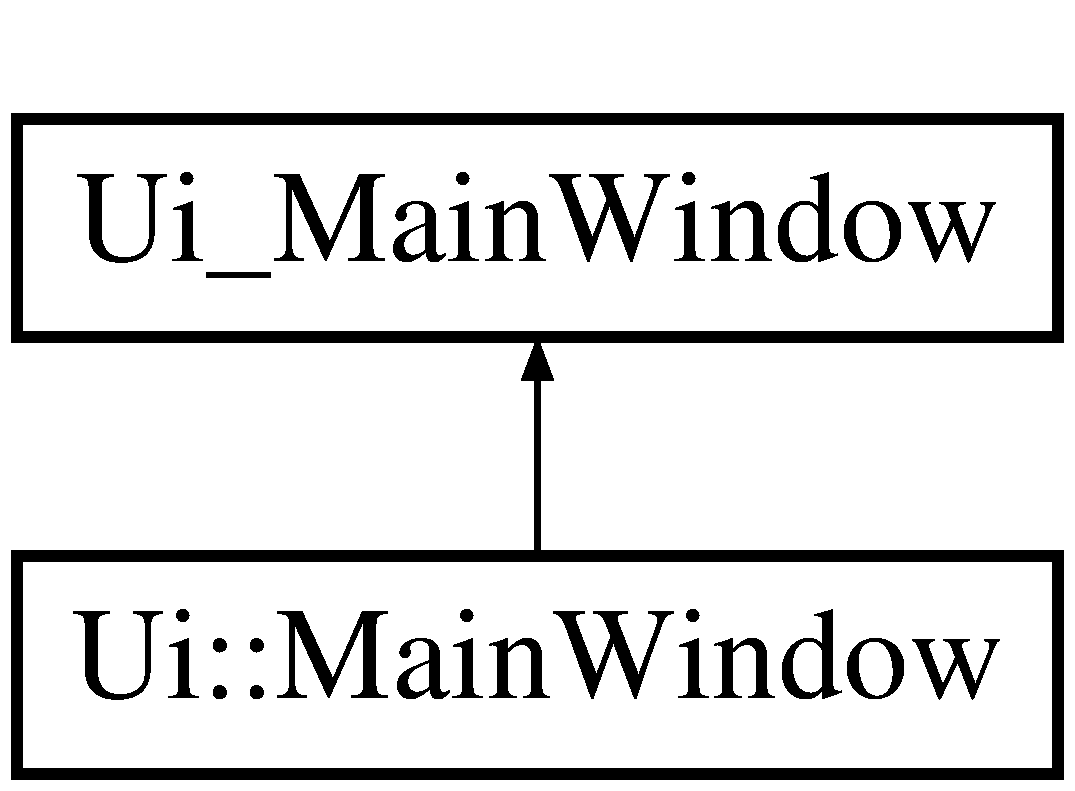
\includegraphics[height=2.000000cm]{class_ui___main_window}
\end{center}
\end{figure}
\subsection*{Public Member Functions}
\begin{DoxyCompactItemize}
\item 
void \hyperlink{class_ui___main_window_acf4a0872c4c77d8f43a2ec66ed849b58}{setup\-Ui} (Q\-Main\-Window $\ast$Main\-Window)
\item 
void \hyperlink{class_ui___main_window_a097dd160c3534a204904cb374412c618}{retranslate\-Ui} (Q\-Main\-Window $\ast$Main\-Window)
\end{DoxyCompactItemize}
\subsection*{Public Attributes}
\begin{DoxyCompactItemize}
\item 
Q\-Widget $\ast$ \hyperlink{class_ui___main_window_a30075506c2116c3ed4ff25e07ae75f81}{central\-Widget}
\item 
Q\-Widget $\ast$ \hyperlink{class_ui___main_window_a805d415fff07a22a85219e1f22f2da28}{vertical\-Layout\-Widget}
\item 
Q\-V\-Box\-Layout $\ast$ \hyperlink{class_ui___main_window_aecd96a04789fcfec3f98d80390ad8184}{vertical\-Layout}
\item 
Q\-Push\-Button $\ast$ \hyperlink{class_ui___main_window_ad332d93084584930878f1daf5f84cdbf}{push\-Button}
\item 
Q\-Menu\-Bar $\ast$ \hyperlink{class_ui___main_window_a2be1c24ec9adfca18e1dcc951931457f}{menu\-Bar}
\item 
Q\-Menu $\ast$ \hyperlink{class_ui___main_window_a7f4ea012695a9e61eb752b30df4caa38}{menu\-Words\-\_\-for\-\_\-\-C\-S\-\_\-340\-\_\-\-Students}
\item 
Q\-Tool\-Bar $\ast$ \hyperlink{class_ui___main_window_a5172877001c8c7b4e0f6de50421867d1}{main\-Tool\-Bar}
\item 
Q\-Status\-Bar $\ast$ \hyperlink{class_ui___main_window_a50fa481337604bcc8bf68de18ab16ecd}{status\-Bar}
\end{DoxyCompactItemize}


\subsection{Detailed Description}


Definition at line 28 of file ui\-\_\-mainwindow.\-h.



\subsection{Member Function Documentation}
\hypertarget{class_ui___main_window_a097dd160c3534a204904cb374412c618}{\index{Ui\-\_\-\-Main\-Window@{Ui\-\_\-\-Main\-Window}!retranslate\-Ui@{retranslate\-Ui}}
\index{retranslate\-Ui@{retranslate\-Ui}!Ui_MainWindow@{Ui\-\_\-\-Main\-Window}}
\subsubsection[{retranslate\-Ui}]{\setlength{\rightskip}{0pt plus 5cm}void Ui\-\_\-\-Main\-Window\-::retranslate\-Ui (
\begin{DoxyParamCaption}
\item[{Q\-Main\-Window $\ast$}]{Main\-Window}
\end{DoxyParamCaption}
)\hspace{0.3cm}{\ttfamily [inline]}}}\label{class_ui___main_window_a097dd160c3534a204904cb374412c618}


Definition at line 81 of file ui\-\_\-mainwindow.\-h.



References menu\-Words\-\_\-for\-\_\-\-C\-S\-\_\-340\-\_\-\-Students, and push\-Button.



Referenced by setup\-Ui().


\begin{DoxyCode}
82     \{
83         MainWindow->setWindowTitle(QApplication::translate(\textcolor{stringliteral}{"MainWindow"}, \textcolor{stringliteral}{"MainWindow"}, 0));
84         \hyperlink{class_ui___main_window_ad332d93084584930878f1daf5f84cdbf}{pushButton}->setText(QApplication::translate(\textcolor{stringliteral}{"MainWindow"}, \textcolor{stringliteral}{"Start Game"}, 0));
85         \hyperlink{class_ui___main_window_a7f4ea012695a9e61eb752b30df4caa38}{menuWords\_for\_CS\_340\_Students}->setTitle(QApplication::translate(\textcolor{stringliteral}{"
      MainWindow"}, \textcolor{stringliteral}{"Words for CS 340 Students"}, 0));
86     \} \textcolor{comment}{// retranslateUi}
\end{DoxyCode}
\hypertarget{class_ui___main_window_acf4a0872c4c77d8f43a2ec66ed849b58}{\index{Ui\-\_\-\-Main\-Window@{Ui\-\_\-\-Main\-Window}!setup\-Ui@{setup\-Ui}}
\index{setup\-Ui@{setup\-Ui}!Ui_MainWindow@{Ui\-\_\-\-Main\-Window}}
\subsubsection[{setup\-Ui}]{\setlength{\rightskip}{0pt plus 5cm}void Ui\-\_\-\-Main\-Window\-::setup\-Ui (
\begin{DoxyParamCaption}
\item[{Q\-Main\-Window $\ast$}]{Main\-Window}
\end{DoxyParamCaption}
)\hspace{0.3cm}{\ttfamily [inline]}}}\label{class_ui___main_window_acf4a0872c4c77d8f43a2ec66ed849b58}


Definition at line 40 of file ui\-\_\-mainwindow.\-h.



References central\-Widget, main\-Tool\-Bar, menu\-Bar, menu\-Words\-\_\-for\-\_\-\-C\-S\-\_\-340\-\_\-\-Students, push\-Button, retranslate\-Ui(), status\-Bar, vertical\-Layout, and vertical\-Layout\-Widget.


\begin{DoxyCode}
41     \{
42         \textcolor{keywordflow}{if} (MainWindow->objectName().isEmpty())
43             MainWindow->setObjectName(QStringLiteral(\textcolor{stringliteral}{"MainWindow"}));
44         MainWindow->resize(826, 469);
45         MainWindow->setMinimumSize(QSize(826, 0));
46         MainWindow->setMaximumSize(QSize(826, 16777215));
47         \hyperlink{class_ui___main_window_a30075506c2116c3ed4ff25e07ae75f81}{centralWidget} = \textcolor{keyword}{new} QWidget(MainWindow);
48         \hyperlink{class_ui___main_window_a30075506c2116c3ed4ff25e07ae75f81}{centralWidget}->setObjectName(QStringLiteral(\textcolor{stringliteral}{"centralWidget"}));
49         \hyperlink{class_ui___main_window_a805d415fff07a22a85219e1f22f2da28}{verticalLayoutWidget} = \textcolor{keyword}{new} QWidget(\hyperlink{class_ui___main_window_a30075506c2116c3ed4ff25e07ae75f81}{centralWidget});
50         \hyperlink{class_ui___main_window_a805d415fff07a22a85219e1f22f2da28}{verticalLayoutWidget}->setObjectName(QStringLiteral(\textcolor{stringliteral}{"verticalLayoutWidget"}));
51         \hyperlink{class_ui___main_window_a805d415fff07a22a85219e1f22f2da28}{verticalLayoutWidget}->setGeometry(QRect(10, 0, 381, 221));
52         \hyperlink{class_ui___main_window_aecd96a04789fcfec3f98d80390ad8184}{verticalLayout} = \textcolor{keyword}{new} QVBoxLayout(\hyperlink{class_ui___main_window_a805d415fff07a22a85219e1f22f2da28}{verticalLayoutWidget});
53         \hyperlink{class_ui___main_window_aecd96a04789fcfec3f98d80390ad8184}{verticalLayout}->setSpacing(6);
54         \hyperlink{class_ui___main_window_aecd96a04789fcfec3f98d80390ad8184}{verticalLayout}->setContentsMargins(11, 11, 11, 11);
55         \hyperlink{class_ui___main_window_aecd96a04789fcfec3f98d80390ad8184}{verticalLayout}->setObjectName(QStringLiteral(\textcolor{stringliteral}{"verticalLayout"}));
56         \hyperlink{class_ui___main_window_aecd96a04789fcfec3f98d80390ad8184}{verticalLayout}->setContentsMargins(0, 0, 0, 0);
57         \hyperlink{class_ui___main_window_ad332d93084584930878f1daf5f84cdbf}{pushButton} = \textcolor{keyword}{new} QPushButton(\hyperlink{class_ui___main_window_a30075506c2116c3ed4ff25e07ae75f81}{centralWidget});
58         \hyperlink{class_ui___main_window_ad332d93084584930878f1daf5f84cdbf}{pushButton}->setObjectName(QStringLiteral(\textcolor{stringliteral}{"pushButton"}));
59         \hyperlink{class_ui___main_window_ad332d93084584930878f1daf5f84cdbf}{pushButton}->setGeometry(QRect(350, 390, 99, 27));
60         MainWindow->setCentralWidget(\hyperlink{class_ui___main_window_a30075506c2116c3ed4ff25e07ae75f81}{centralWidget});
61         \hyperlink{class_ui___main_window_a2be1c24ec9adfca18e1dcc951931457f}{menuBar} = \textcolor{keyword}{new} QMenuBar(MainWindow);
62         \hyperlink{class_ui___main_window_a2be1c24ec9adfca18e1dcc951931457f}{menuBar}->setObjectName(QStringLiteral(\textcolor{stringliteral}{"menuBar"}));
63         \hyperlink{class_ui___main_window_a2be1c24ec9adfca18e1dcc951931457f}{menuBar}->setGeometry(QRect(0, 0, 826, 25));
64         \hyperlink{class_ui___main_window_a7f4ea012695a9e61eb752b30df4caa38}{menuWords\_for\_CS\_340\_Students} = \textcolor{keyword}{new} QMenu(
      \hyperlink{class_ui___main_window_a2be1c24ec9adfca18e1dcc951931457f}{menuBar});
65         \hyperlink{class_ui___main_window_a7f4ea012695a9e61eb752b30df4caa38}{menuWords\_for\_CS\_340\_Students}->setObjectName(QStringLiteral(\textcolor{stringliteral}{"
      menuWords\_for\_CS\_340\_Students"}));
66         MainWindow->setMenuBar(\hyperlink{class_ui___main_window_a2be1c24ec9adfca18e1dcc951931457f}{menuBar});
67         \hyperlink{class_ui___main_window_a5172877001c8c7b4e0f6de50421867d1}{mainToolBar} = \textcolor{keyword}{new} QToolBar(MainWindow);
68         \hyperlink{class_ui___main_window_a5172877001c8c7b4e0f6de50421867d1}{mainToolBar}->setObjectName(QStringLiteral(\textcolor{stringliteral}{"mainToolBar"}));
69         MainWindow->addToolBar(Qt::TopToolBarArea, \hyperlink{class_ui___main_window_a5172877001c8c7b4e0f6de50421867d1}{mainToolBar});
70         \hyperlink{class_ui___main_window_a50fa481337604bcc8bf68de18ab16ecd}{statusBar} = \textcolor{keyword}{new} QStatusBar(MainWindow);
71         \hyperlink{class_ui___main_window_a50fa481337604bcc8bf68de18ab16ecd}{statusBar}->setObjectName(QStringLiteral(\textcolor{stringliteral}{"statusBar"}));
72         MainWindow->setStatusBar(\hyperlink{class_ui___main_window_a50fa481337604bcc8bf68de18ab16ecd}{statusBar});
73 
74         \hyperlink{class_ui___main_window_a2be1c24ec9adfca18e1dcc951931457f}{menuBar}->addAction(\hyperlink{class_ui___main_window_a7f4ea012695a9e61eb752b30df4caa38}{menuWords\_for\_CS\_340\_Students}->menuAction())
      ;
75 
76         \hyperlink{class_ui___main_window_a097dd160c3534a204904cb374412c618}{retranslateUi}(MainWindow);
77 
78         QMetaObject::connectSlotsByName(MainWindow);
79     \} \textcolor{comment}{// setupUi}
\end{DoxyCode}


\subsection{Member Data Documentation}
\hypertarget{class_ui___main_window_a30075506c2116c3ed4ff25e07ae75f81}{\index{Ui\-\_\-\-Main\-Window@{Ui\-\_\-\-Main\-Window}!central\-Widget@{central\-Widget}}
\index{central\-Widget@{central\-Widget}!Ui_MainWindow@{Ui\-\_\-\-Main\-Window}}
\subsubsection[{central\-Widget}]{\setlength{\rightskip}{0pt plus 5cm}Q\-Widget$\ast$ Ui\-\_\-\-Main\-Window\-::central\-Widget}}\label{class_ui___main_window_a30075506c2116c3ed4ff25e07ae75f81}


Definition at line 31 of file ui\-\_\-mainwindow.\-h.



Referenced by setup\-Ui().

\hypertarget{class_ui___main_window_a5172877001c8c7b4e0f6de50421867d1}{\index{Ui\-\_\-\-Main\-Window@{Ui\-\_\-\-Main\-Window}!main\-Tool\-Bar@{main\-Tool\-Bar}}
\index{main\-Tool\-Bar@{main\-Tool\-Bar}!Ui_MainWindow@{Ui\-\_\-\-Main\-Window}}
\subsubsection[{main\-Tool\-Bar}]{\setlength{\rightskip}{0pt plus 5cm}Q\-Tool\-Bar$\ast$ Ui\-\_\-\-Main\-Window\-::main\-Tool\-Bar}}\label{class_ui___main_window_a5172877001c8c7b4e0f6de50421867d1}


Definition at line 37 of file ui\-\_\-mainwindow.\-h.



Referenced by setup\-Ui().

\hypertarget{class_ui___main_window_a2be1c24ec9adfca18e1dcc951931457f}{\index{Ui\-\_\-\-Main\-Window@{Ui\-\_\-\-Main\-Window}!menu\-Bar@{menu\-Bar}}
\index{menu\-Bar@{menu\-Bar}!Ui_MainWindow@{Ui\-\_\-\-Main\-Window}}
\subsubsection[{menu\-Bar}]{\setlength{\rightskip}{0pt plus 5cm}Q\-Menu\-Bar$\ast$ Ui\-\_\-\-Main\-Window\-::menu\-Bar}}\label{class_ui___main_window_a2be1c24ec9adfca18e1dcc951931457f}


Definition at line 35 of file ui\-\_\-mainwindow.\-h.



Referenced by setup\-Ui().

\hypertarget{class_ui___main_window_a7f4ea012695a9e61eb752b30df4caa38}{\index{Ui\-\_\-\-Main\-Window@{Ui\-\_\-\-Main\-Window}!menu\-Words\-\_\-for\-\_\-\-C\-S\-\_\-340\-\_\-\-Students@{menu\-Words\-\_\-for\-\_\-\-C\-S\-\_\-340\-\_\-\-Students}}
\index{menu\-Words\-\_\-for\-\_\-\-C\-S\-\_\-340\-\_\-\-Students@{menu\-Words\-\_\-for\-\_\-\-C\-S\-\_\-340\-\_\-\-Students}!Ui_MainWindow@{Ui\-\_\-\-Main\-Window}}
\subsubsection[{menu\-Words\-\_\-for\-\_\-\-C\-S\-\_\-340\-\_\-\-Students}]{\setlength{\rightskip}{0pt plus 5cm}Q\-Menu$\ast$ Ui\-\_\-\-Main\-Window\-::menu\-Words\-\_\-for\-\_\-\-C\-S\-\_\-340\-\_\-\-Students}}\label{class_ui___main_window_a7f4ea012695a9e61eb752b30df4caa38}


Definition at line 36 of file ui\-\_\-mainwindow.\-h.



Referenced by retranslate\-Ui(), and setup\-Ui().

\hypertarget{class_ui___main_window_ad332d93084584930878f1daf5f84cdbf}{\index{Ui\-\_\-\-Main\-Window@{Ui\-\_\-\-Main\-Window}!push\-Button@{push\-Button}}
\index{push\-Button@{push\-Button}!Ui_MainWindow@{Ui\-\_\-\-Main\-Window}}
\subsubsection[{push\-Button}]{\setlength{\rightskip}{0pt plus 5cm}Q\-Push\-Button$\ast$ Ui\-\_\-\-Main\-Window\-::push\-Button}}\label{class_ui___main_window_ad332d93084584930878f1daf5f84cdbf}


Definition at line 34 of file ui\-\_\-mainwindow.\-h.



Referenced by retranslate\-Ui(), and setup\-Ui().

\hypertarget{class_ui___main_window_a50fa481337604bcc8bf68de18ab16ecd}{\index{Ui\-\_\-\-Main\-Window@{Ui\-\_\-\-Main\-Window}!status\-Bar@{status\-Bar}}
\index{status\-Bar@{status\-Bar}!Ui_MainWindow@{Ui\-\_\-\-Main\-Window}}
\subsubsection[{status\-Bar}]{\setlength{\rightskip}{0pt plus 5cm}Q\-Status\-Bar$\ast$ Ui\-\_\-\-Main\-Window\-::status\-Bar}}\label{class_ui___main_window_a50fa481337604bcc8bf68de18ab16ecd}


Definition at line 38 of file ui\-\_\-mainwindow.\-h.



Referenced by setup\-Ui().

\hypertarget{class_ui___main_window_aecd96a04789fcfec3f98d80390ad8184}{\index{Ui\-\_\-\-Main\-Window@{Ui\-\_\-\-Main\-Window}!vertical\-Layout@{vertical\-Layout}}
\index{vertical\-Layout@{vertical\-Layout}!Ui_MainWindow@{Ui\-\_\-\-Main\-Window}}
\subsubsection[{vertical\-Layout}]{\setlength{\rightskip}{0pt plus 5cm}Q\-V\-Box\-Layout$\ast$ Ui\-\_\-\-Main\-Window\-::vertical\-Layout}}\label{class_ui___main_window_aecd96a04789fcfec3f98d80390ad8184}


Definition at line 33 of file ui\-\_\-mainwindow.\-h.



Referenced by setup\-Ui().

\hypertarget{class_ui___main_window_a805d415fff07a22a85219e1f22f2da28}{\index{Ui\-\_\-\-Main\-Window@{Ui\-\_\-\-Main\-Window}!vertical\-Layout\-Widget@{vertical\-Layout\-Widget}}
\index{vertical\-Layout\-Widget@{vertical\-Layout\-Widget}!Ui_MainWindow@{Ui\-\_\-\-Main\-Window}}
\subsubsection[{vertical\-Layout\-Widget}]{\setlength{\rightskip}{0pt plus 5cm}Q\-Widget$\ast$ Ui\-\_\-\-Main\-Window\-::vertical\-Layout\-Widget}}\label{class_ui___main_window_a805d415fff07a22a85219e1f22f2da28}


Definition at line 32 of file ui\-\_\-mainwindow.\-h.



Referenced by setup\-Ui().



The documentation for this class was generated from the following file\-:\begin{DoxyCompactItemize}
\item 
Scrabble/\hyperlink{ui__mainwindow_8h}{ui\-\_\-mainwindow.\-h}\end{DoxyCompactItemize}

\hypertarget{class_unit_test}{\section{Unit\-Test Class Reference}
\label{class_unit_test}\index{Unit\-Test@{Unit\-Test}}
}
\subsection*{Public Member Functions}
\begin{DoxyCompactItemize}
\item 
void \hyperlink{class_unit_test_adab1694e1b8220401e0e8de84146c00c}{dictionarytest} ()
\item 
void \hyperlink{class_unit_test_a72c0f15a7dcecdec8eb882f861e784e2}{runalltests} ()
\end{DoxyCompactItemize}
\subsection*{Private Attributes}
\begin{DoxyCompactItemize}
\item 
\hyperlink{class_dictionary}{Dictionary} $\ast$ \hyperlink{class_unit_test_a09902f0cb75bf2c03c56912ecd4682aa}{dictionary}
\item 
\hyperlink{class_dictionary}{Dictionary} $\ast$ \hyperlink{class_unit_test_a81579d68baa8575bdf1625a0642eadf8}{a\-\_\-dictionary}
\item 
\hyperlink{class_dictionary_loader}{Dictionary\-Loader} $\ast$ \hyperlink{class_unit_test_a9cf46138e9006b18b978f6a3126c8c50}{dictionary\-Loader}
\item 
list$<$ Q\-String $>$ $\ast$ \hyperlink{class_unit_test_aeb6acd51a206123112b000f6520ac25b}{wordlist}
\item 
list$<$ Q\-String $>$ $\ast$ \hyperlink{class_unit_test_aeb6e626c75d7caa5100aa605831a439f}{anagramlist}
\end{DoxyCompactItemize}
\subsection*{Static Private Attributes}
\begin{DoxyCompactItemize}
\item 
static const unsigned int \hyperlink{class_unit_test_a9e7b7ee73cb31ffb5b98bbb69a0aa999}{anagramcount} = 168
\end{DoxyCompactItemize}


\subsection{Detailed Description}


Definition at line 12 of file Unit\-Test.\-cpp.



\subsection{Member Function Documentation}
\hypertarget{class_unit_test_adab1694e1b8220401e0e8de84146c00c}{\index{Unit\-Test@{Unit\-Test}!dictionarytest@{dictionarytest}}
\index{dictionarytest@{dictionarytest}!UnitTest@{Unit\-Test}}
\subsubsection[{dictionarytest}]{\setlength{\rightskip}{0pt plus 5cm}void Unit\-Test\-::dictionarytest (
\begin{DoxyParamCaption}
{}
\end{DoxyParamCaption}
)\hspace{0.3cm}{\ttfamily [inline]}}}\label{class_unit_test_adab1694e1b8220401e0e8de84146c00c}


Definition at line 22 of file Unit\-Test.\-cpp.



References a\-\_\-dictionary, Trie\-::ai\-\_\-search(), anagramcount, anagramlist, Trie\-::anagrams(), dictionary, dictionary\-Loader, Dictionary\-::is\-Word(), Dictionary\-Loader\-::load(), Dictionary\-::wordcount(), wordlist, and Dictionary\-::words.



Referenced by runalltests().


\begin{DoxyCode}
23     \{
24         \textcolor{comment}{/*}
25 \textcolor{comment}{         *  Basic Dictionary checks. Can we load it, and does it contain some very basic words?}
26 \textcolor{comment}{         */}
27         \hyperlink{class_unit_test_a09902f0cb75bf2c03c56912ecd4682aa}{dictionary} = \textcolor{keyword}{new} \hyperlink{class_dictionary}{Dictionary}();
28         \hyperlink{class_unit_test_a9cf46138e9006b18b978f6a3126c8c50}{dictionaryLoader} = \textcolor{keyword}{new} \hyperlink{class_dictionary_loader}{DictionaryLoader}(
      \hyperlink{class_unit_test_a09902f0cb75bf2c03c56912ecd4682aa}{dictionary}, \textcolor{stringliteral}{":/resources/dictionary.txt"});
29         \hyperlink{class_unit_test_a9cf46138e9006b18b978f6a3126c8c50}{dictionaryLoader}->\hyperlink{class_dictionary_loader_a1441785d7f5a848be0d7b7f432e338f8}{load}();
30 
31         assert(\hyperlink{class_unit_test_a09902f0cb75bf2c03c56912ecd4682aa}{dictionary}->\hyperlink{class_dictionary_a327b99a18977f2b898adfd496426cf27}{wordcount}());
32         assert(\hyperlink{class_unit_test_a09902f0cb75bf2c03c56912ecd4682aa}{dictionary}->\hyperlink{class_dictionary_afe2588ce04f6ad733c51df58a8d0d96b}{isWord}(\textcolor{stringliteral}{"a"}));
33         assert(\hyperlink{class_unit_test_a09902f0cb75bf2c03c56912ecd4682aa}{dictionary}->\hyperlink{class_dictionary_afe2588ce04f6ad733c51df58a8d0d96b}{isWord}(\textcolor{stringliteral}{"aa"}));
34         assert(\hyperlink{class_unit_test_a09902f0cb75bf2c03c56912ecd4682aa}{dictionary}->\hyperlink{class_dictionary_afe2588ce04f6ad733c51df58a8d0d96b}{isWord}(\textcolor{stringliteral}{"aardvark"}));
35         assert(\hyperlink{class_unit_test_a09902f0cb75bf2c03c56912ecd4682aa}{dictionary}->\hyperlink{class_dictionary_afe2588ce04f6ad733c51df58a8d0d96b}{isWord}(\textcolor{stringliteral}{"blue"}));
36         assert(\hyperlink{class_unit_test_a09902f0cb75bf2c03c56912ecd4682aa}{dictionary}->\hyperlink{class_dictionary_afe2588ce04f6ad733c51df58a8d0d96b}{isWord}(\textcolor{stringliteral}{"cow"}));
37         assert(\hyperlink{class_unit_test_a09902f0cb75bf2c03c56912ecd4682aa}{dictionary}->\hyperlink{class_dictionary_afe2588ce04f6ad733c51df58a8d0d96b}{isWord}(\textcolor{stringliteral}{"pie"}));
38 
39 
40         \textcolor{comment}{/*                      ANAGRAM TESTS}
41 \textcolor{comment}{         *}
42 \textcolor{comment}{         *  The word 'nameless' has a lot of anagrams. Let's see if we have all of them.}
43 \textcolor{comment}{         *  The anagram file inserted is \_required\_ to contain only unique anagrams.}
44 \textcolor{comment}{         *}
45 \textcolor{comment}{         */}
46 
47         \hyperlink{class_unit_test_a81579d68baa8575bdf1625a0642eadf8}{a\_dictionary} = \textcolor{keyword}{new} \hyperlink{class_dictionary}{Dictionary}();
48         \textcolor{keyword}{delete} \hyperlink{class_unit_test_a9cf46138e9006b18b978f6a3126c8c50}{dictionaryLoader};
49         \hyperlink{class_unit_test_a9cf46138e9006b18b978f6a3126c8c50}{dictionaryLoader} = \textcolor{keyword}{new} \hyperlink{class_dictionary_loader}{DictionaryLoader}(a\_dictionary, \textcolor{stringliteral}{"
      :/resources/nameless\_anagrams.txt"});
50         \hyperlink{class_unit_test_a9cf46138e9006b18b978f6a3126c8c50}{dictionaryLoader}->\hyperlink{class_dictionary_loader_a1441785d7f5a848be0d7b7f432e338f8}{load}();
51 
52         \hyperlink{class_unit_test_aeb6acd51a206123112b000f6520ac25b}{wordlist} = \textcolor{keyword}{new} list<QString>();
53         \hyperlink{class_unit_test_aeb6e626c75d7caa5100aa605831a439f}{anagramlist} = \textcolor{keyword}{new} list<QString>();
54         \hyperlink{class_unit_test_a09902f0cb75bf2c03c56912ecd4682aa}{dictionary}->\hyperlink{class_dictionary_ac6c08127a37d8131fb8fb1e738406e85}{words}->\hyperlink{class_trie_aa42c01330538b67e0aff76068f02a8f7}{anagrams}(\textcolor{stringliteral}{"nameless"},\hyperlink{class_unit_test_aeb6acd51a206123112b000f6520ac25b}{wordlist});
55 
56         \textcolor{comment}{// This should return equal to the wordcount found in the anagram file.}
57         a\_dictionary->words->anagrams(\textcolor{stringliteral}{"nameless"},anagramlist);
58         assert(anagramlist->size() == \hyperlink{class_unit_test_a9e7b7ee73cb31ffb5b98bbb69a0aa999}{anagramcount});
59 
60         cout << \textcolor{stringliteral}{"wordlist: "} << \hyperlink{class_unit_test_aeb6acd51a206123112b000f6520ac25b}{wordlist}->size() << endl;
61         cout << \textcolor{stringliteral}{"anaglist: "} << anagramlist->size() << endl;
62 
63         list<QString> * wildanagramlist = \textcolor{keyword}{new} list<QString>();
64         \hyperlink{class_unit_test_a09902f0cb75bf2c03c56912ecd4682aa}{dictionary}->\hyperlink{class_dictionary_ac6c08127a37d8131fb8fb1e738406e85}{words}->\hyperlink{class_trie_aa42c01330538b67e0aff76068f02a8f7}{anagrams}(\textcolor{stringliteral}{"hel**"},wildanagramlist);
65         \textcolor{keywordflow}{for} (std::list<QString>::iterator it = wildanagramlist->begin(); it != wildanagramlist->end(); it++
      )
66         \{
67             assert(\hyperlink{class_unit_test_a09902f0cb75bf2c03c56912ecd4682aa}{dictionary}->\hyperlink{class_dictionary_afe2588ce04f6ad733c51df58a8d0d96b}{isWord}(*it));
68             cout << QString(*it).toStdString() << endl;
69         \}
70 
71         \textcolor{comment}{/*}
72 \textcolor{comment}{         *}
73 \textcolor{comment}{         * We now have a vector of words containing all the anagrams for the word}
74 \textcolor{comment}{         * 'nameless' that are found in our dictionary. Let's assure that we have them}
75 \textcolor{comment}{         * all. And more importantly, that we don't have false positives.}
76 \textcolor{comment}{         *}
77 \textcolor{comment}{         *}
78 \textcolor{comment}{         * Let's compare sizes first! This is a very basic test.}
79 \textcolor{comment}{         * nameless\_anagrams.txt is not a \_complete\_ list.}
80 \textcolor{comment}{         * However, we do assume that the dictionary is big enough that it should contain most of these.}
81 \textcolor{comment}{         *}
82 \textcolor{comment}{         */}
83 
84         assert( \hyperlink{class_unit_test_aeb6acd51a206123112b000f6520ac25b}{wordlist}->size() >= anagramlist->size() && \hyperlink{class_unit_test_aeb6acd51a206123112b000f6520ac25b}{wordlist}->size() <= 2 * 
      anagramlist->size() );
85 
86         \textcolor{keywordflow}{for} (std::list<QString>::iterator it = anagramlist->begin(); it != anagramlist->end(); it++)
87             assert(\hyperlink{class_unit_test_a09902f0cb75bf2c03c56912ecd4682aa}{dictionary}->\hyperlink{class_dictionary_afe2588ce04f6ad733c51df58a8d0d96b}{isWord}(*it));
88 
89         \textcolor{comment}{// We have now confirmed that all the words in the anagramlist are in the anagrams found}
90         \textcolor{comment}{// in the dictionary.}
91 
92         QRegularExpression *re = \textcolor{keyword}{new} QRegularExpression(\textcolor{stringliteral}{"^[a-zA-Z*]+$"});
93         assert(re->match(QString(\textcolor{stringliteral}{"abcdefghijklmnopqrstuvwxyz*"}),0,QRegularExpression::NormalMatch,
      QRegularExpression::NoMatchOption ).hasMatch());
94 
95         \textcolor{comment}{// A confirmation that our basic PCRE regexp works. Also used as a reference.}
96 
97         \textcolor{comment}{// Standard anchored ai search. The first position is the anchor.}
98         list<QString> * newwordlist = \textcolor{keyword}{new} list<QString>();
99         \hyperlink{class_unit_test_a09902f0cb75bf2c03c56912ecd4682aa}{dictionary}->\hyperlink{class_dictionary_ac6c08127a37d8131fb8fb1e738406e85}{words}->\hyperlink{class_trie_ac6a915f9483d03dc99872210b74bf435}{ai\_search}(\textcolor{stringliteral}{"nameless"},\textcolor{stringliteral}{"*a*e*ess*"},newwordlist);
100         \textcolor{keywordflow}{for} (std::list<QString>::iterator it = newwordlist->begin(); it != newwordlist->end(); it++)
101             assert(\hyperlink{class_unit_test_a09902f0cb75bf2c03c56912ecd4682aa}{dictionary}->\hyperlink{class_dictionary_afe2588ce04f6ad733c51df58a8d0d96b}{isWord}(*it));
102 
103         \textcolor{comment}{/* Can we do all of these deletions succesfully? */}
104         \textcolor{keyword}{delete} \hyperlink{class_unit_test_aeb6acd51a206123112b000f6520ac25b}{wordlist};
105         \textcolor{keyword}{delete} \hyperlink{class_unit_test_a9cf46138e9006b18b978f6a3126c8c50}{dictionaryLoader};
106         \textcolor{keyword}{delete} \hyperlink{class_unit_test_a09902f0cb75bf2c03c56912ecd4682aa}{dictionary};
107     \}
\end{DoxyCode}
\hypertarget{class_unit_test_a72c0f15a7dcecdec8eb882f861e784e2}{\index{Unit\-Test@{Unit\-Test}!runalltests@{runalltests}}
\index{runalltests@{runalltests}!UnitTest@{Unit\-Test}}
\subsubsection[{runalltests}]{\setlength{\rightskip}{0pt plus 5cm}void Unit\-Test\-::runalltests (
\begin{DoxyParamCaption}
{}
\end{DoxyParamCaption}
)\hspace{0.3cm}{\ttfamily [inline]}}}\label{class_unit_test_a72c0f15a7dcecdec8eb882f861e784e2}


Definition at line 109 of file Unit\-Test.\-cpp.



References dictionarytest().



Referenced by main().


\begin{DoxyCode}
110     \{
111         \hyperlink{class_unit_test_adab1694e1b8220401e0e8de84146c00c}{dictionarytest}();
112     \}
\end{DoxyCode}


\subsection{Member Data Documentation}
\hypertarget{class_unit_test_a81579d68baa8575bdf1625a0642eadf8}{\index{Unit\-Test@{Unit\-Test}!a\-\_\-dictionary@{a\-\_\-dictionary}}
\index{a\-\_\-dictionary@{a\-\_\-dictionary}!UnitTest@{Unit\-Test}}
\subsubsection[{a\-\_\-dictionary}]{\setlength{\rightskip}{0pt plus 5cm}{\bf Dictionary}$\ast$ Unit\-Test\-::a\-\_\-dictionary\hspace{0.3cm}{\ttfamily [private]}}}\label{class_unit_test_a81579d68baa8575bdf1625a0642eadf8}


Definition at line 15 of file Unit\-Test.\-cpp.



Referenced by dictionarytest().

\hypertarget{class_unit_test_a9e7b7ee73cb31ffb5b98bbb69a0aa999}{\index{Unit\-Test@{Unit\-Test}!anagramcount@{anagramcount}}
\index{anagramcount@{anagramcount}!UnitTest@{Unit\-Test}}
\subsubsection[{anagramcount}]{\setlength{\rightskip}{0pt plus 5cm}const unsigned int Unit\-Test\-::anagramcount = 168\hspace{0.3cm}{\ttfamily [static]}, {\ttfamily [private]}}}\label{class_unit_test_a9e7b7ee73cb31ffb5b98bbb69a0aa999}


Definition at line 19 of file Unit\-Test.\-cpp.



Referenced by dictionarytest().

\hypertarget{class_unit_test_aeb6e626c75d7caa5100aa605831a439f}{\index{Unit\-Test@{Unit\-Test}!anagramlist@{anagramlist}}
\index{anagramlist@{anagramlist}!UnitTest@{Unit\-Test}}
\subsubsection[{anagramlist}]{\setlength{\rightskip}{0pt plus 5cm}list$<$Q\-String$>$$\ast$ Unit\-Test\-::anagramlist\hspace{0.3cm}{\ttfamily [private]}}}\label{class_unit_test_aeb6e626c75d7caa5100aa605831a439f}


Definition at line 18 of file Unit\-Test.\-cpp.



Referenced by dictionarytest().

\hypertarget{class_unit_test_a09902f0cb75bf2c03c56912ecd4682aa}{\index{Unit\-Test@{Unit\-Test}!dictionary@{dictionary}}
\index{dictionary@{dictionary}!UnitTest@{Unit\-Test}}
\subsubsection[{dictionary}]{\setlength{\rightskip}{0pt plus 5cm}{\bf Dictionary}$\ast$ Unit\-Test\-::dictionary\hspace{0.3cm}{\ttfamily [private]}}}\label{class_unit_test_a09902f0cb75bf2c03c56912ecd4682aa}


Definition at line 14 of file Unit\-Test.\-cpp.



Referenced by dictionarytest().

\hypertarget{class_unit_test_a9cf46138e9006b18b978f6a3126c8c50}{\index{Unit\-Test@{Unit\-Test}!dictionary\-Loader@{dictionary\-Loader}}
\index{dictionary\-Loader@{dictionary\-Loader}!UnitTest@{Unit\-Test}}
\subsubsection[{dictionary\-Loader}]{\setlength{\rightskip}{0pt plus 5cm}{\bf Dictionary\-Loader}$\ast$ Unit\-Test\-::dictionary\-Loader\hspace{0.3cm}{\ttfamily [private]}}}\label{class_unit_test_a9cf46138e9006b18b978f6a3126c8c50}


Definition at line 16 of file Unit\-Test.\-cpp.



Referenced by dictionarytest().

\hypertarget{class_unit_test_aeb6acd51a206123112b000f6520ac25b}{\index{Unit\-Test@{Unit\-Test}!wordlist@{wordlist}}
\index{wordlist@{wordlist}!UnitTest@{Unit\-Test}}
\subsubsection[{wordlist}]{\setlength{\rightskip}{0pt plus 5cm}list$<$Q\-String$>$$\ast$ Unit\-Test\-::wordlist\hspace{0.3cm}{\ttfamily [private]}}}\label{class_unit_test_aeb6acd51a206123112b000f6520ac25b}


Definition at line 17 of file Unit\-Test.\-cpp.



Referenced by dictionarytest().



The documentation for this class was generated from the following file\-:\begin{DoxyCompactItemize}
\item 
Scrabble/\hyperlink{_unit_test_8cpp}{Unit\-Test.\-cpp}\end{DoxyCompactItemize}

\chapter{File Documentation}
\hypertarget{aiplayer_8cpp}{\section{Scrabble/aiplayer.cpp File Reference}
\label{aiplayer_8cpp}\index{Scrabble/aiplayer.\-cpp@{Scrabble/aiplayer.\-cpp}}
}
{\ttfamily \#include \char`\"{}aiplayer.\-h\char`\"{}}\\*
{\ttfamily \#include \char`\"{}assert.\-h\char`\"{}}\\*
{\ttfamily \#include $<$cctype$>$}\\*
\subsection*{Functions}
\begin{DoxyCompactItemize}
\item 
bool \hyperlink{aiplayer_8cpp_a5ec041e0f53c78a5b4267c3df32ee188}{\-\_\-pred\-\_\-value\-\_\-sort} (\hyperlink{class_play}{Play} $\ast$a, \hyperlink{class_play}{Play} $\ast$b)
\end{DoxyCompactItemize}


\subsection{Function Documentation}
\hypertarget{aiplayer_8cpp_a5ec041e0f53c78a5b4267c3df32ee188}{\index{aiplayer.\-cpp@{aiplayer.\-cpp}!\-\_\-pred\-\_\-value\-\_\-sort@{\-\_\-pred\-\_\-value\-\_\-sort}}
\index{\-\_\-pred\-\_\-value\-\_\-sort@{\-\_\-pred\-\_\-value\-\_\-sort}!aiplayer.cpp@{aiplayer.\-cpp}}
\subsubsection[{\-\_\-pred\-\_\-value\-\_\-sort}]{\setlength{\rightskip}{0pt plus 5cm}bool \-\_\-pred\-\_\-value\-\_\-sort (
\begin{DoxyParamCaption}
\item[{{\bf Play} $\ast$}]{a, }
\item[{{\bf Play} $\ast$}]{b}
\end{DoxyParamCaption}
)}}\label{aiplayer_8cpp_a5ec041e0f53c78a5b4267c3df32ee188}


Definition at line 42 of file aiplayer.\-cpp.



References Play\-::get\-Value().



Referenced by A\-I\-Player\-::play().


\begin{DoxyCode}
43 \{
44     \textcolor{keywordflow}{return} a->\hyperlink{class_play_af2599835f6eba8136770a4f773a9f9ef}{getValue}() > b->\hyperlink{class_play_af2599835f6eba8136770a4f773a9f9ef}{getValue}();
45 \}
\end{DoxyCode}

\hypertarget{aiplayer_8h}{\section{Scrabble/aiplayer.h File Reference}
\label{aiplayer_8h}\index{Scrabble/aiplayer.\-h@{Scrabble/aiplayer.\-h}}
}
{\ttfamily \#include \char`\"{}board.\-h\char`\"{}}\\*
{\ttfamily \#include \char`\"{}player.\-h\char`\"{}}\\*
{\ttfamily \#include \char`\"{}move.\-h\char`\"{}}\\*
\subsection*{Classes}
\begin{DoxyCompactItemize}
\item 
class \hyperlink{class_a_i_player}{A\-I\-Player}
\end{DoxyCompactItemize}

\hypertarget{board_8cpp}{\section{Scrabble/board.cpp File Reference}
\label{board_8cpp}\index{Scrabble/board.\-cpp@{Scrabble/board.\-cpp}}
}
{\ttfamily \#include $<$stdlib.\-h$>$}\\*
{\ttfamily \#include \char`\"{}board.\-h\char`\"{}}\\*
{\ttfamily \#include $<$Q\-Layout$>$}\\*
{\ttfamily \#include $<$Q\-Push\-Button$>$}\\*
{\ttfamily \#include \char`\"{}assert.\-h\char`\"{}}\\*
\subsection*{Functions}
\begin{DoxyCompactItemize}
\item 
ostream \& \hyperlink{board_8cpp_ad799faa7c15b047d09f3fa52406c95d5}{operator$<$$<$} (ostream \&os, const \hyperlink{class_board}{Board} \&board)
\begin{DoxyCompactList}\small\item\em operator $<$$<$ Overloading the $<$$<$ operator for debugging information \end{DoxyCompactList}\end{DoxyCompactItemize}


\subsection{Function Documentation}
\hypertarget{board_8cpp_ad799faa7c15b047d09f3fa52406c95d5}{\index{board.\-cpp@{board.\-cpp}!operator$<$$<$@{operator$<$$<$}}
\index{operator$<$$<$@{operator$<$$<$}!board.cpp@{board.\-cpp}}
\subsubsection[{operator$<$$<$}]{\setlength{\rightskip}{0pt plus 5cm}ostream\& operator$<$$<$ (
\begin{DoxyParamCaption}
\item[{ostream \&}]{os, }
\item[{const {\bf Board} \&}]{board}
\end{DoxyParamCaption}
)}}\label{board_8cpp_ad799faa7c15b047d09f3fa52406c95d5}


operator $<$$<$ Overloading the $<$$<$ operator for debugging information 


\begin{DoxyParams}{Parameters}
{\em os} & The output stream \\
\hline
{\em board} & The board to be output \\
\hline
\end{DoxyParams}
\begin{DoxyReturn}{Returns}
The modified output stream 
\end{DoxyReturn}


Definition at line 804 of file board.\-cpp.



References B\-O\-A\-R\-D\-S\-I\-Z\-E, and Board\-::spaces.


\begin{DoxyCode}
805 \{
806     \textcolor{keywordflow}{for}(\textcolor{keywordtype}{int} i = 0; i < \hyperlink{board_8h_afb909c1a2193edc88c68390c025b2fa7}{BOARDSIZE}; i++) \{
807         cout << \textcolor{stringliteral}{"\{"} << setw(2) << i << \textcolor{stringliteral}{"\}"};
808         \textcolor{keywordflow}{for}(\textcolor{keywordtype}{int} j = 0; j < \hyperlink{board_8h_afb909c1a2193edc88c68390c025b2fa7}{BOARDSIZE}; j++) \{
809             os << *(board.\hyperlink{class_board_a73b12248ddb6ee3adc24f4458d8661c2}{spaces}[i][j]);
810         \}
811         os << endl;
812     \}
813     cout << \textcolor{stringliteral}{"\{XX\}\{0 \}\{1 \}\{2 \}\{3 \}\{4 \}\{5 \}\{6 \}\{7 \}\{8 \}\{9 \}\{10\}\{11\}\{12\}\{13\}\{14\}"};
814     \textcolor{keywordflow}{return} os;
815 \}
\end{DoxyCode}

\hypertarget{board_8h}{\section{Scrabble/board.h File Reference}
\label{board_8h}\index{Scrabble/board.\-h@{Scrabble/board.\-h}}
}
{\ttfamily \#include $<$vector$>$}\\*
{\ttfamily \#include $<$iostream$>$}\\*
{\ttfamily \#include $<$Q\-Object$>$}\\*
{\ttfamily \#include $<$iomanip$>$}\\*
{\ttfamily \#include \char`\"{}space.\-h\char`\"{}}\\*
{\ttfamily \#include \char`\"{}rack.\-h\char`\"{}}\\*
{\ttfamily \#include \char`\"{}game.\-h\char`\"{}}\\*
{\ttfamily \#include \char`\"{}play.\-h\char`\"{}}\\*
\subsection*{Classes}
\begin{DoxyCompactItemize}
\item 
class \hyperlink{class_board}{Board}
\begin{DoxyCompactList}\small\item\em The \hyperlink{class_board}{Board} class Singleton that represents a playing board. \end{DoxyCompactList}\end{DoxyCompactItemize}
\subsection*{Variables}
\begin{DoxyCompactItemize}
\item 
static const int \hyperlink{board_8h_afb909c1a2193edc88c68390c025b2fa7}{B\-O\-A\-R\-D\-S\-I\-Z\-E} = 15
\item 
static const Q\-String \hyperlink{board_8h_a55a5e2b160827afd2651003878573e48}{T\-R\-I\-P\-L\-E\-W\-O\-R\-D\-C\-O\-L\-O\-R} = \char`\"{}pink\char`\"{}
\item 
static const Q\-String \hyperlink{board_8h_a52e9b32f92467d14351e5a500f48638f}{T\-R\-I\-P\-L\-E\-L\-E\-T\-T\-E\-R\-C\-O\-L\-O\-R} = \char`\"{}lightblue\char`\"{}
\item 
static const Q\-String \hyperlink{board_8h_a10e5d0be9a98901f142735d07e5537f6}{D\-O\-U\-B\-L\-E\-W\-O\-R\-D\-C\-O\-L\-O\-R} = \char`\"{}mistyrose\char`\"{}
\item 
static const Q\-String \hyperlink{board_8h_ae1643176725e430fda174728d157a635}{D\-O\-U\-B\-L\-E\-L\-E\-T\-T\-E\-R\-C\-O\-L\-O\-R} = \char`\"{}lightskyblue\char`\"{}
\end{DoxyCompactItemize}


\subsection{Variable Documentation}
\hypertarget{board_8h_afb909c1a2193edc88c68390c025b2fa7}{\index{board.\-h@{board.\-h}!B\-O\-A\-R\-D\-S\-I\-Z\-E@{B\-O\-A\-R\-D\-S\-I\-Z\-E}}
\index{B\-O\-A\-R\-D\-S\-I\-Z\-E@{B\-O\-A\-R\-D\-S\-I\-Z\-E}!board.h@{board.\-h}}
\subsubsection[{B\-O\-A\-R\-D\-S\-I\-Z\-E}]{\setlength{\rightskip}{0pt plus 5cm}const int B\-O\-A\-R\-D\-S\-I\-Z\-E = 15\hspace{0.3cm}{\ttfamily [static]}}}\label{board_8h_afb909c1a2193edc88c68390c025b2fa7}
The size of the board (it is 15 x 15 spaces 

Definition at line 16 of file board.\-h.



Referenced by Board\-::are\-Valid\-Words(), Board\-::\-Board(), Board\-::has\-New(), Board\-::inactivate\-Other\-Spaces(), Board\-::is\-Touching\-On\-Board(), Board\-::must\-Touch\-Column(), Board\-::must\-Touch\-Row(), Board\-::no\-Column\-Blanks(), Board\-::no\-Row\-Blanks(), Board\-::on\-\_\-cancel\-Button\-\_\-clicked(), operator$<$$<$(), Board\-::reset(), Board\-::same\-Row\-Or\-Column(), Board\-::score\-Horizontal(), Board\-::score\-Horizontal\-Word(), Board\-::score\-Vertical(), Board\-::score\-Vertical\-Word(), Board\-::set\-Space(), Board\-::setup\-Plain\-Spaces(), Board\-::validate\-Word\-Horizontal(), Board\-::validate\-Word\-Vertical(), and Board\-::$\sim$\-Board().

\hypertarget{board_8h_ae1643176725e430fda174728d157a635}{\index{board.\-h@{board.\-h}!D\-O\-U\-B\-L\-E\-L\-E\-T\-T\-E\-R\-C\-O\-L\-O\-R@{D\-O\-U\-B\-L\-E\-L\-E\-T\-T\-E\-R\-C\-O\-L\-O\-R}}
\index{D\-O\-U\-B\-L\-E\-L\-E\-T\-T\-E\-R\-C\-O\-L\-O\-R@{D\-O\-U\-B\-L\-E\-L\-E\-T\-T\-E\-R\-C\-O\-L\-O\-R}!board.h@{board.\-h}}
\subsubsection[{D\-O\-U\-B\-L\-E\-L\-E\-T\-T\-E\-R\-C\-O\-L\-O\-R}]{\setlength{\rightskip}{0pt plus 5cm}const Q\-String D\-O\-U\-B\-L\-E\-L\-E\-T\-T\-E\-R\-C\-O\-L\-O\-R = \char`\"{}lightskyblue\char`\"{}\hspace{0.3cm}{\ttfamily [static]}}}\label{board_8h_ae1643176725e430fda174728d157a635}
The color for double letter spaces 

Definition at line 21 of file board.\-h.



Referenced by Board\-::setup2\-L().

\hypertarget{board_8h_a10e5d0be9a98901f142735d07e5537f6}{\index{board.\-h@{board.\-h}!D\-O\-U\-B\-L\-E\-W\-O\-R\-D\-C\-O\-L\-O\-R@{D\-O\-U\-B\-L\-E\-W\-O\-R\-D\-C\-O\-L\-O\-R}}
\index{D\-O\-U\-B\-L\-E\-W\-O\-R\-D\-C\-O\-L\-O\-R@{D\-O\-U\-B\-L\-E\-W\-O\-R\-D\-C\-O\-L\-O\-R}!board.h@{board.\-h}}
\subsubsection[{D\-O\-U\-B\-L\-E\-W\-O\-R\-D\-C\-O\-L\-O\-R}]{\setlength{\rightskip}{0pt plus 5cm}const Q\-String D\-O\-U\-B\-L\-E\-W\-O\-R\-D\-C\-O\-L\-O\-R = \char`\"{}mistyrose\char`\"{}\hspace{0.3cm}{\ttfamily [static]}}}\label{board_8h_a10e5d0be9a98901f142735d07e5537f6}
The color for double word spaces 

Definition at line 20 of file board.\-h.



Referenced by Board\-::setup2\-W(), and Board\-::setup\-Start().

\hypertarget{board_8h_a52e9b32f92467d14351e5a500f48638f}{\index{board.\-h@{board.\-h}!T\-R\-I\-P\-L\-E\-L\-E\-T\-T\-E\-R\-C\-O\-L\-O\-R@{T\-R\-I\-P\-L\-E\-L\-E\-T\-T\-E\-R\-C\-O\-L\-O\-R}}
\index{T\-R\-I\-P\-L\-E\-L\-E\-T\-T\-E\-R\-C\-O\-L\-O\-R@{T\-R\-I\-P\-L\-E\-L\-E\-T\-T\-E\-R\-C\-O\-L\-O\-R}!board.h@{board.\-h}}
\subsubsection[{T\-R\-I\-P\-L\-E\-L\-E\-T\-T\-E\-R\-C\-O\-L\-O\-R}]{\setlength{\rightskip}{0pt plus 5cm}const Q\-String T\-R\-I\-P\-L\-E\-L\-E\-T\-T\-E\-R\-C\-O\-L\-O\-R = \char`\"{}lightblue\char`\"{}\hspace{0.3cm}{\ttfamily [static]}}}\label{board_8h_a52e9b32f92467d14351e5a500f48638f}
The color for triple letter spaces 

Definition at line 19 of file board.\-h.



Referenced by Board\-::setup3\-L().

\hypertarget{board_8h_a55a5e2b160827afd2651003878573e48}{\index{board.\-h@{board.\-h}!T\-R\-I\-P\-L\-E\-W\-O\-R\-D\-C\-O\-L\-O\-R@{T\-R\-I\-P\-L\-E\-W\-O\-R\-D\-C\-O\-L\-O\-R}}
\index{T\-R\-I\-P\-L\-E\-W\-O\-R\-D\-C\-O\-L\-O\-R@{T\-R\-I\-P\-L\-E\-W\-O\-R\-D\-C\-O\-L\-O\-R}!board.h@{board.\-h}}
\subsubsection[{T\-R\-I\-P\-L\-E\-W\-O\-R\-D\-C\-O\-L\-O\-R}]{\setlength{\rightskip}{0pt plus 5cm}const Q\-String T\-R\-I\-P\-L\-E\-W\-O\-R\-D\-C\-O\-L\-O\-R = \char`\"{}pink\char`\"{}\hspace{0.3cm}{\ttfamily [static]}}}\label{board_8h_a55a5e2b160827afd2651003878573e48}
The color for triple word spaces 

Definition at line 18 of file board.\-h.



Referenced by Board\-::setup3\-W().


\hypertarget{dialog_8cpp}{\section{Scrabble/dialog.cpp File Reference}
\label{dialog_8cpp}\index{Scrabble/dialog.\-cpp@{Scrabble/dialog.\-cpp}}
}
{\ttfamily \#include $<$Q\-V\-Box\-Layout$>$}\\*
{\ttfamily \#include $<$Q\-Push\-Button$>$}\\*
{\ttfamily \#include $<$Q\-Form\-Layout$>$}\\*
{\ttfamily \#include $<$Q\-Spin\-Box$>$}\\*
{\ttfamily \#include $<$Q\-Combo\-Box$>$}\\*
{\ttfamily \#include \char`\"{}dialog.\-h\char`\"{}}\\*
{\ttfamily \#include \char`\"{}playerlabel.\-h\char`\"{}}\\*

\hypertarget{dialog_8h}{\section{Scrabble/dialog.h File Reference}
\label{dialog_8h}\index{Scrabble/dialog.\-h@{Scrabble/dialog.\-h}}
}
{\ttfamily \#include $<$Q\-Dialog$>$}\\*
{\ttfamily \#include $<$Q\-Menu\-Bar$>$}\\*
{\ttfamily \#include $<$Q\-Group\-Box$>$}\\*
{\ttfamily \#include $<$Q\-Text\-Edit$>$}\\*
{\ttfamily \#include $<$Q\-Label$>$}\\*
{\ttfamily \#include $<$Q\-Line\-Edit$>$}\\*
{\ttfamily \#include $<$Q\-Dialog\-Button\-Box$>$}\\*
{\ttfamily \#include \char`\"{}dictionary.\-h\char`\"{}}\\*
{\ttfamily \#include \char`\"{}dictionaryloader.\-h\char`\"{}}\\*
{\ttfamily \#include \char`\"{}humanplayer.\-h\char`\"{}}\\*
{\ttfamily \#include \char`\"{}aiplayer.\-h\char`\"{}}\\*
{\ttfamily \#include \char`\"{}game.\-h\char`\"{}}\\*
{\ttfamily \#include \char`\"{}rack.\-h\char`\"{}}\\*
\subsection*{Classes}
\begin{DoxyCompactItemize}
\item 
class \hyperlink{class_dialog}{Dialog}
\begin{DoxyCompactList}\small\item\em The \hyperlink{class_dialog}{Dialog} class Main U\-I class. \end{DoxyCompactList}\end{DoxyCompactItemize}

\hypertarget{dictionary_8cpp}{\section{Scrabble/dictionary.cpp File Reference}
\label{dictionary_8cpp}\index{Scrabble/dictionary.\-cpp@{Scrabble/dictionary.\-cpp}}
}
{\ttfamily \#include \char`\"{}dictionary.\-h\char`\"{}}\\*

\hypertarget{dictionary_8h}{\section{Scrabble/dictionary.h File Reference}
\label{dictionary_8h}\index{Scrabble/dictionary.\-h@{Scrabble/dictionary.\-h}}
}
{\ttfamily \#include $<$Q\-Hash$>$}\\*
{\ttfamily \#include \char`\"{}trie.\-h\char`\"{}}\\*
{\ttfamily \#include $<$qstring.\-h$>$}\\*
\subsection*{Classes}
\begin{DoxyCompactItemize}
\item 
class \hyperlink{class_dictionary}{Dictionary}
\begin{DoxyCompactList}\small\item\em The \hyperlink{class_dictionary}{Dictionary} class Encapsulates dicitonary operations. \end{DoxyCompactList}\end{DoxyCompactItemize}

\hypertarget{dictionaryloader_8cpp}{\section{Scrabble/dictionaryloader.cpp File Reference}
\label{dictionaryloader_8cpp}\index{Scrabble/dictionaryloader.\-cpp@{Scrabble/dictionaryloader.\-cpp}}
}
{\ttfamily \#include $<$Q\-File$>$}\\*
{\ttfamily \#include $<$Q\-Text\-Stream$>$}\\*
{\ttfamily \#include $<$iostream$>$}\\*
{\ttfamily \#include \char`\"{}dictionaryloader.\-h\char`\"{}}\\*

\hypertarget{dictionaryloader_8h}{\section{Scrabble/dictionaryloader.h File Reference}
\label{dictionaryloader_8h}\index{Scrabble/dictionaryloader.\-h@{Scrabble/dictionaryloader.\-h}}
}
{\ttfamily \#include $<$qstring.\-h$>$}\\*
{\ttfamily \#include \char`\"{}dictionary.\-h\char`\"{}}\\*
\subsection*{Classes}
\begin{DoxyCompactItemize}
\item 
class \hyperlink{class_dictionary_loader}{Dictionary\-Loader}
\begin{DoxyCompactList}\small\item\em The \hyperlink{class_dictionary_loader}{Dictionary\-Loader} class Loads a file of words into the dictionary. \end{DoxyCompactList}\end{DoxyCompactItemize}

\hypertarget{game_8cpp}{\section{Scrabble/game.cpp File Reference}
\label{game_8cpp}\index{Scrabble/game.\-cpp@{Scrabble/game.\-cpp}}
}
{\ttfamily \#include \char`\"{}game.\-h\char`\"{}}\\*
{\ttfamily \#include $<$assert.\-h$>$}\\*
{\ttfamily \#include \char`\"{}aiplayer.\-h\char`\"{}}\\*
\subsection*{Functions}
\begin{DoxyCompactItemize}
\item 
ostream \& \hyperlink{game_8cpp_a41c0344e76853337b335ed0cb6df12ec}{operator$<$$<$} (ostream \&os, const \hyperlink{class_game}{Game} \&game)
\begin{DoxyCompactList}\small\item\em operator $<$$<$ Overloading the $<$$<$ operator for debugging information \end{DoxyCompactList}\end{DoxyCompactItemize}


\subsection{Function Documentation}
\hypertarget{game_8cpp_a41c0344e76853337b335ed0cb6df12ec}{\index{game.\-cpp@{game.\-cpp}!operator$<$$<$@{operator$<$$<$}}
\index{operator$<$$<$@{operator$<$$<$}!game.cpp@{game.\-cpp}}
\subsubsection[{operator$<$$<$}]{\setlength{\rightskip}{0pt plus 5cm}ostream\& operator$<$$<$ (
\begin{DoxyParamCaption}
\item[{ostream \&}]{os, }
\item[{const {\bf Game} \&}]{game}
\end{DoxyParamCaption}
)}}\label{game_8cpp_a41c0344e76853337b335ed0cb6df12ec}


operator $<$$<$ Overloading the $<$$<$ operator for debugging information 


\begin{DoxyParams}{Parameters}
{\em os} & The output stream \\
\hline
{\em game} & The game object \\
\hline
\end{DoxyParams}
\begin{DoxyReturn}{Returns}
The modified output stream 
\end{DoxyReturn}


Definition at line 90 of file game.\-cpp.



References Board\-::get\-Board(), and Game\-::num\-Players.


\begin{DoxyCode}
90                                                    \{
91     os << \textcolor{stringliteral}{"This is a "} << game.\hyperlink{class_game_a7c03c2f209dfde4ef01c739b050159f6}{numPlayers} << \textcolor{stringliteral}{" player game."} << endl;
92     os << *(\hyperlink{class_board_ae30e802b1d83309fc95e695b5b3df338}{Board::getBoard}());
93     \textcolor{keywordflow}{return} os;
94 \}
\end{DoxyCode}

\hypertarget{game_8h}{\section{Scrabble/game.h File Reference}
\label{game_8h}\index{Scrabble/game.\-h@{Scrabble/game.\-h}}
}
{\ttfamily \#include $<$iostream$>$}\\*
{\ttfamily \#include \char`\"{}dictionary.\-h\char`\"{}}\\*
{\ttfamily \#include \char`\"{}player.\-h\char`\"{}}\\*
{\ttfamily \#include \char`\"{}board.\-h\char`\"{}}\\*
{\ttfamily \#include \char`\"{}letterpool.\-h\char`\"{}}\\*
{\ttfamily \#include \char`\"{}play.\-h\char`\"{}}\\*
\subsection*{Classes}
\begin{DoxyCompactItemize}
\item 
class \hyperlink{class_game}{Game}
\begin{DoxyCompactList}\small\item\em The \hyperlink{class_game}{Game} class Encapsulates a game. \end{DoxyCompactList}\end{DoxyCompactItemize}
\subsection*{Variables}
\begin{DoxyCompactItemize}
\item 
static const int \hyperlink{game_8h_a11b26774d4c310f3cbd649bd1a645b5a}{M\-A\-X\-P\-L\-A\-Y\-E\-R\-S} = 4
\end{DoxyCompactItemize}


\subsection{Variable Documentation}
\hypertarget{game_8h_a11b26774d4c310f3cbd649bd1a645b5a}{\index{game.\-h@{game.\-h}!M\-A\-X\-P\-L\-A\-Y\-E\-R\-S@{M\-A\-X\-P\-L\-A\-Y\-E\-R\-S}}
\index{M\-A\-X\-P\-L\-A\-Y\-E\-R\-S@{M\-A\-X\-P\-L\-A\-Y\-E\-R\-S}!game.h@{game.\-h}}
\subsubsection[{M\-A\-X\-P\-L\-A\-Y\-E\-R\-S}]{\setlength{\rightskip}{0pt plus 5cm}const int M\-A\-X\-P\-L\-A\-Y\-E\-R\-S = 4\hspace{0.3cm}{\ttfamily [static]}}}\label{game_8h_a11b26774d4c310f3cbd649bd1a645b5a}
The maximum number of players 

Definition at line 15 of file game.\-h.


\hypertarget{humanplayer_8cpp}{\section{Scrabble/humanplayer.cpp File Reference}
\label{humanplayer_8cpp}\index{Scrabble/humanplayer.\-cpp@{Scrabble/humanplayer.\-cpp}}
}
{\ttfamily \#include \char`\"{}humanplayer.\-h\char`\"{}}\\*

\hypertarget{humanplayer_8h}{\section{Scrabble/humanplayer.h File Reference}
\label{humanplayer_8h}\index{Scrabble/humanplayer.\-h@{Scrabble/humanplayer.\-h}}
}
{\ttfamily \#include \char`\"{}player.\-h\char`\"{}}\\*
\subsection*{Classes}
\begin{DoxyCompactItemize}
\item 
class \hyperlink{class_human_player}{Human\-Player}
\begin{DoxyCompactList}\small\item\em The \hyperlink{class_human_player}{Human\-Player} class Human playable \hyperlink{class_player}{Player}. \end{DoxyCompactList}\end{DoxyCompactItemize}

\hypertarget{letter_8cpp}{\section{Scrabble/letter.cpp File Reference}
\label{letter_8cpp}\index{Scrabble/letter.\-cpp@{Scrabble/letter.\-cpp}}
}
{\ttfamily \#include $<$iostream$>$}\\*
{\ttfamily \#include \char`\"{}letter.\-h\char`\"{}}\\*
\subsection*{Functions}
\begin{DoxyCompactItemize}
\item 
ostream \& \hyperlink{letter_8cpp_a90f2b9e82cfd5e6c60087fb6c1f92937}{operator$<$$<$} (ostream \&os, const \hyperlink{class_letter}{Letter} \&letter)
\begin{DoxyCompactList}\small\item\em operator $<$$<$ Overloaded ostream operator \end{DoxyCompactList}\end{DoxyCompactItemize}


\subsection{Function Documentation}
\hypertarget{letter_8cpp_a90f2b9e82cfd5e6c60087fb6c1f92937}{\index{letter.\-cpp@{letter.\-cpp}!operator$<$$<$@{operator$<$$<$}}
\index{operator$<$$<$@{operator$<$$<$}!letter.cpp@{letter.\-cpp}}
\subsubsection[{operator$<$$<$}]{\setlength{\rightskip}{0pt plus 5cm}ostream\& operator$<$$<$ (
\begin{DoxyParamCaption}
\item[{ostream \&}]{os, }
\item[{const {\bf Letter} \&}]{letter}
\end{DoxyParamCaption}
)}}\label{letter_8cpp_a90f2b9e82cfd5e6c60087fb6c1f92937}


operator $<$$<$ Overloaded ostream operator 


\begin{DoxyParams}{Parameters}
{\em os} & The ostream \\
\hline
{\em letter} & The letter \\
\hline
\end{DoxyParams}
\begin{DoxyReturn}{Returns}
The modified ostream 
\end{DoxyReturn}


Definition at line 104 of file letter.\-cpp.



References Letter\-::letter.


\begin{DoxyCode}
104                                                        \{
105     os << letter.\hyperlink{class_letter_a430f7ba15c252da3874f641422090fbd}{letter}.toLatin1();
106     \textcolor{keywordflow}{return} os;
107 \}
\end{DoxyCode}

\hypertarget{letter_8h}{\section{Scrabble/letter.h File Reference}
\label{letter_8h}\index{Scrabble/letter.\-h@{Scrabble/letter.\-h}}
}
{\ttfamily \#include $<$Q\-Char$>$}\\*
{\ttfamily \#include $<$iostream$>$}\\*
\subsection*{Classes}
\begin{DoxyCompactItemize}
\item 
class \hyperlink{class_letter}{Letter}
\begin{DoxyCompactList}\small\item\em The \hyperlink{class_letter}{Letter} class Encapsulates a \hyperlink{class_letter}{Letter} (or Tile) \end{DoxyCompactList}\end{DoxyCompactItemize}

\hypertarget{letterpool_8cpp}{\section{Scrabble/letterpool.cpp File Reference}
\label{letterpool_8cpp}\index{Scrabble/letterpool.\-cpp@{Scrabble/letterpool.\-cpp}}
}
{\ttfamily \#include \char`\"{}letterpool.\-h\char`\"{}}\\*

\hypertarget{letterpool_8h}{\section{Scrabble/letterpool.h File Reference}
\label{letterpool_8h}\index{Scrabble/letterpool.\-h@{Scrabble/letterpool.\-h}}
}
{\ttfamily \#include \char`\"{}letter.\-h\char`\"{}}\\*
{\ttfamily \#include \char`\"{}iostream\char`\"{}}\\*
{\ttfamily \#include $<$Q\-Vector$>$}\\*
{\ttfamily \#include $<$stdlib.\-h$>$}\\*
{\ttfamily \#include $<$time.\-h$>$}\\*
\subsection*{Classes}
\begin{DoxyCompactItemize}
\item 
class \hyperlink{class_letter_pool}{Letter\-Pool}
\begin{DoxyCompactList}\small\item\em The \hyperlink{class_letter_pool}{Letter\-Pool} class Holds the letters not already in play. \end{DoxyCompactList}\end{DoxyCompactItemize}

\hypertarget{main_8cpp}{\section{Scrabble/main.cpp File Reference}
\label{main_8cpp}\index{Scrabble/main.\-cpp@{Scrabble/main.\-cpp}}
}
{\ttfamily \#include $<$Q\-Application$>$}\\*
{\ttfamily \#include $<$Q\-Debug$>$}\\*
{\ttfamily \#include $<$iostream$>$}\\*
{\ttfamily \#include $<$qscreen.\-h$>$}\\*
{\ttfamily \#include \char`\"{}dictionaryloader.\-h\char`\"{}}\\*
{\ttfamily \#include \char`\"{}game.\-h\char`\"{}}\\*
{\ttfamily \#include \char`\"{}humanplayer.\-h\char`\"{}}\\*
{\ttfamily \#include $<$Q\-Layout$>$}\\*
{\ttfamily \#include $<$Q\-Push\-Button$>$}\\*
{\ttfamily \#include $<$Q\-String$>$}\\*
{\ttfamily \#include $<$Q\-Splitter$>$}\\*
{\ttfamily \#include $<$Q\-Dock\-Widget$>$}\\*
{\ttfamily \#include \char`\"{}dialog.\-h\char`\"{}}\\*
{\ttfamily \#include \char`\"{}Unit\-Test.\-cpp\char`\"{}}\\*
\subsection*{Functions}
\begin{DoxyCompactItemize}
\item 
int \hyperlink{main_8cpp_a0ddf1224851353fc92bfbff6f499fa97}{main} (int argc, char $\ast$argv\mbox{[}$\,$\mbox{]})
\begin{DoxyCompactList}\small\item\em main Main \end{DoxyCompactList}\end{DoxyCompactItemize}
\subsection*{Variables}
\begin{DoxyCompactItemize}
\item 
static const bool \hyperlink{main_8cpp_a94b2b3683b77a25673da9c79a6e00160}{U\-N\-I\-T\-T\-E\-S\-T} = false
\item 
static const int \hyperlink{main_8cpp_ace32d8fe826ab9598e69afbf5ba01605}{X\-S\-I\-Z\-E} = 700
\item 
static const int \hyperlink{main_8cpp_ad232391ce8fa869d9df10a8faff06c49}{Y\-S\-I\-Z\-E} = 700
\end{DoxyCompactItemize}


\subsection{Function Documentation}
\hypertarget{main_8cpp_a0ddf1224851353fc92bfbff6f499fa97}{\index{main.\-cpp@{main.\-cpp}!main@{main}}
\index{main@{main}!main.cpp@{main.\-cpp}}
\subsubsection[{main}]{\setlength{\rightskip}{0pt plus 5cm}int main (
\begin{DoxyParamCaption}
\item[{int}]{argc, }
\item[{char $\ast$}]{argv\mbox{[}$\,$\mbox{]}}
\end{DoxyParamCaption}
)}}\label{main_8cpp_a0ddf1224851353fc92bfbff6f499fa97}


main Main 


\begin{DoxyParams}{Parameters}
{\em argc} & The argument count \\
\hline
{\em argv} & The argument values \\
\hline
\end{DoxyParams}
\begin{DoxyReturn}{Returns}
0 if no errors 
\end{DoxyReturn}


Definition at line 29 of file main.\-cpp.



References Unit\-Test\-::runalltests(), and U\-N\-I\-T\-T\-E\-S\-T.


\begin{DoxyCode}
30 \{
31     \textcolor{comment}{// Run unit tests}
32     \textcolor{keywordflow}{if}( \hyperlink{main_8cpp_a94b2b3683b77a25673da9c79a6e00160}{UNITTEST} == \textcolor{keyword}{true} )
33     \{
34         \hyperlink{class_unit_test}{UnitTest} * tester = \textcolor{keyword}{new} \hyperlink{class_unit_test}{UnitTest}();
35         tester->\hyperlink{class_unit_test_a72c0f15a7dcecdec8eb882f861e784e2}{runalltests}();
36         \textcolor{keyword}{delete} tester;
37     \}
38 
39     \textcolor{comment}{// Run the application}
40     QApplication a(argc, argv);
41     \hyperlink{class_dialog}{Dialog} *dialog = \textcolor{keyword}{new} \hyperlink{class_dialog}{Dialog};
42     dialog->show();
43 
44     \textcolor{keywordflow}{return} a.exec();
45 \}
\end{DoxyCode}


\subsection{Variable Documentation}
\hypertarget{main_8cpp_a94b2b3683b77a25673da9c79a6e00160}{\index{main.\-cpp@{main.\-cpp}!U\-N\-I\-T\-T\-E\-S\-T@{U\-N\-I\-T\-T\-E\-S\-T}}
\index{U\-N\-I\-T\-T\-E\-S\-T@{U\-N\-I\-T\-T\-E\-S\-T}!main.cpp@{main.\-cpp}}
\subsubsection[{U\-N\-I\-T\-T\-E\-S\-T}]{\setlength{\rightskip}{0pt plus 5cm}const bool U\-N\-I\-T\-T\-E\-S\-T = false\hspace{0.3cm}{\ttfamily [static]}}}\label{main_8cpp_a94b2b3683b77a25673da9c79a6e00160}


Definition at line 16 of file main.\-cpp.



Referenced by main().

\hypertarget{main_8cpp_ace32d8fe826ab9598e69afbf5ba01605}{\index{main.\-cpp@{main.\-cpp}!X\-S\-I\-Z\-E@{X\-S\-I\-Z\-E}}
\index{X\-S\-I\-Z\-E@{X\-S\-I\-Z\-E}!main.cpp@{main.\-cpp}}
\subsubsection[{X\-S\-I\-Z\-E}]{\setlength{\rightskip}{0pt plus 5cm}const int X\-S\-I\-Z\-E = 700\hspace{0.3cm}{\ttfamily [static]}}}\label{main_8cpp_ace32d8fe826ab9598e69afbf5ba01605}


Definition at line 20 of file main.\-cpp.

\hypertarget{main_8cpp_ad232391ce8fa869d9df10a8faff06c49}{\index{main.\-cpp@{main.\-cpp}!Y\-S\-I\-Z\-E@{Y\-S\-I\-Z\-E}}
\index{Y\-S\-I\-Z\-E@{Y\-S\-I\-Z\-E}!main.cpp@{main.\-cpp}}
\subsubsection[{Y\-S\-I\-Z\-E}]{\setlength{\rightskip}{0pt plus 5cm}const int Y\-S\-I\-Z\-E = 700\hspace{0.3cm}{\ttfamily [static]}}}\label{main_8cpp_ad232391ce8fa869d9df10a8faff06c49}


Definition at line 21 of file main.\-cpp.


\hypertarget{mainpage_8dox}{\section{Scrabble/mainpage.dox File Reference}
\label{mainpage_8dox}\index{Scrabble/mainpage.\-dox@{Scrabble/mainpage.\-dox}}
}

\hypertarget{move_8cpp}{\section{Scrabble/move.cpp File Reference}
\label{move_8cpp}\index{Scrabble/move.\-cpp@{Scrabble/move.\-cpp}}
}
{\ttfamily \#include \char`\"{}move.\-h\char`\"{}}\\*

\hypertarget{move_8h}{\section{Scrabble/move.h File Reference}
\label{move_8h}\index{Scrabble/move.\-h@{Scrabble/move.\-h}}
}
{\ttfamily \#include \char`\"{}player.\-h\char`\"{}}\\*
{\ttfamily \#include \char`\"{}letter.\-h\char`\"{}}\\*
{\ttfamily \#include \char`\"{}space.\-h\char`\"{}}\\*
\subsection*{Classes}
\begin{DoxyCompactItemize}
\item 
class \hyperlink{class_move}{Move}
\begin{DoxyCompactList}\small\item\em The \hyperlink{class_move}{Move} class Contains a single move from a \hyperlink{class_rack}{Rack} to the \hyperlink{class_board}{Board}. \end{DoxyCompactList}\end{DoxyCompactItemize}

\hypertarget{play_8cpp}{\section{Scrabble/play.cpp File Reference}
\label{play_8cpp}\index{Scrabble/play.\-cpp@{Scrabble/play.\-cpp}}
}
{\ttfamily \#include \char`\"{}play.\-h\char`\"{}}\\*

\hypertarget{play_8h}{\section{Scrabble/play.h File Reference}
\label{play_8h}\index{Scrabble/play.\-h@{Scrabble/play.\-h}}
}
{\ttfamily \#include \char`\"{}player.\-h\char`\"{}}\\*
{\ttfamily \#include \char`\"{}letter.\-h\char`\"{}}\\*
{\ttfamily \#include \char`\"{}board.\-h\char`\"{}}\\*
{\ttfamily \#include \char`\"{}move.\-h\char`\"{}}\\*
{\ttfamily \#include $<$Q\-List$>$}\\*
\subsection*{Classes}
\begin{DoxyCompactItemize}
\item 
class \hyperlink{class_play}{Play}
\begin{DoxyCompactList}\small\item\em The \hyperlink{class_play}{Play} class Wrapper for a set of Moves that make up a \hyperlink{class_play}{Play}. \end{DoxyCompactList}\end{DoxyCompactItemize}

\hypertarget{player_8cpp}{\section{Scrabble/player.cpp File Reference}
\label{player_8cpp}\index{Scrabble/player.\-cpp@{Scrabble/player.\-cpp}}
}
{\ttfamily \#include \char`\"{}player.\-h\char`\"{}}\\*
\subsection*{Functions}
\begin{DoxyCompactItemize}
\item 
ostream \& \hyperlink{player_8cpp_a79571356003607b80edc6440c851e503}{operator$<$$<$} (ostream \&os, const \hyperlink{class_player}{Player} \&player)
\begin{DoxyCompactList}\small\item\em operator $<$$<$ Overloaded operator for \hyperlink{class_player}{Player}\& \end{DoxyCompactList}\end{DoxyCompactItemize}


\subsection{Function Documentation}
\hypertarget{player_8cpp_a79571356003607b80edc6440c851e503}{\index{player.\-cpp@{player.\-cpp}!operator$<$$<$@{operator$<$$<$}}
\index{operator$<$$<$@{operator$<$$<$}!player.cpp@{player.\-cpp}}
\subsubsection[{operator$<$$<$}]{\setlength{\rightskip}{0pt plus 5cm}ostream\& operator$<$$<$ (
\begin{DoxyParamCaption}
\item[{ostream \&}]{os, }
\item[{const {\bf Player} \&}]{player}
\end{DoxyParamCaption}
)}}\label{player_8cpp_a79571356003607b80edc6440c851e503}


operator $<$$<$ Overloaded operator for \hyperlink{class_player}{Player}\& 


\begin{DoxyParams}{Parameters}
{\em os} & The ostream \\
\hline
{\em player} & The player \\
\hline
\end{DoxyParams}
\begin{DoxyReturn}{Returns}
The modified ostream 
\end{DoxyReturn}


Definition at line 188 of file player.\-cpp.



References Player\-::letters.


\begin{DoxyCode}
188                                                        \{
189     \textcolor{keywordflow}{for}(\textcolor{keywordtype}{unsigned} \textcolor{keywordtype}{int} i = 0; i < player.\hyperlink{class_player_abd40dc8f6d524bd1331a8133e9bb8902}{letters}.size(); i++) \{
190         os << *(player.\hyperlink{class_player_abd40dc8f6d524bd1331a8133e9bb8902}{letters}[i]);
191     \}
192     \textcolor{keywordflow}{return} os;
193 \}
\end{DoxyCode}

\hypertarget{player_8h}{\section{Scrabble/player.h File Reference}
\label{player_8h}\index{Scrabble/player.\-h@{Scrabble/player.\-h}}
}
{\ttfamily \#include $<$Q\-String$>$}\\*
{\ttfamily \#include $<$vector$>$}\\*
{\ttfamily \#include \char`\"{}letter.\-h\char`\"{}}\\*
{\ttfamily \#include \char`\"{}dictionary.\-h\char`\"{}}\\*
{\ttfamily \#include \char`\"{}board.\-h\char`\"{}}\\*
{\ttfamily \#include \char`\"{}letterpool.\-h\char`\"{}}\\*
{\ttfamily \#include \char`\"{}play.\-h\char`\"{}}\\*
\subsection*{Classes}
\begin{DoxyCompactItemize}
\item 
class \hyperlink{class_player}{Player}
\begin{DoxyCompactList}\small\item\em The \hyperlink{class_player}{Player} class Abstract class representing a \hyperlink{class_player}{Player}. \end{DoxyCompactList}\end{DoxyCompactItemize}
\subsection*{Variables}
\begin{DoxyCompactItemize}
\item 
static const int \hyperlink{player_8h_a65437be5d7abb586fe7338331e988e01}{M\-A\-X\-T\-I\-L\-E\-S\-I\-N\-H\-A\-N\-D} = 7
\end{DoxyCompactItemize}


\subsection{Variable Documentation}
\hypertarget{player_8h_a65437be5d7abb586fe7338331e988e01}{\index{player.\-h@{player.\-h}!M\-A\-X\-T\-I\-L\-E\-S\-I\-N\-H\-A\-N\-D@{M\-A\-X\-T\-I\-L\-E\-S\-I\-N\-H\-A\-N\-D}}
\index{M\-A\-X\-T\-I\-L\-E\-S\-I\-N\-H\-A\-N\-D@{M\-A\-X\-T\-I\-L\-E\-S\-I\-N\-H\-A\-N\-D}!player.h@{player.\-h}}
\subsubsection[{M\-A\-X\-T\-I\-L\-E\-S\-I\-N\-H\-A\-N\-D}]{\setlength{\rightskip}{0pt plus 5cm}const int M\-A\-X\-T\-I\-L\-E\-S\-I\-N\-H\-A\-N\-D = 7\hspace{0.3cm}{\ttfamily [static]}}}\label{player_8h_a65437be5d7abb586fe7338331e988e01}


Definition at line 12 of file player.\-h.



Referenced by Player\-::add\-Letter(), and Player\-::fill\-Letters().


\hypertarget{playerlabel_8cpp}{\section{Scrabble/playerlabel.cpp File Reference}
\label{playerlabel_8cpp}\index{Scrabble/playerlabel.\-cpp@{Scrabble/playerlabel.\-cpp}}
}
{\ttfamily \#include \char`\"{}playerlabel.\-h\char`\"{}}\\*

\hypertarget{playerlabel_8h}{\section{Scrabble/playerlabel.h File Reference}
\label{playerlabel_8h}\index{Scrabble/playerlabel.\-h@{Scrabble/playerlabel.\-h}}
}
{\ttfamily \#include $<$Q\-Label$>$}\\*
{\ttfamily \#include $<$Q\-Widget$>$}\\*
{\ttfamily \#include \char`\"{}player.\-h\char`\"{}}\\*
\subsection*{Classes}
\begin{DoxyCompactItemize}
\item 
class \hyperlink{class_player_label}{Player\-Label}
\begin{DoxyCompactList}\small\item\em The \hyperlink{class_player_label}{Player\-Label} class Represents the \hyperlink{class_player}{Player} within the \hyperlink{class_dialog}{Dialog}. \end{DoxyCompactList}\end{DoxyCompactItemize}

\hypertarget{rack_8cpp}{\section{Scrabble/rack.cpp File Reference}
\label{rack_8cpp}\index{Scrabble/rack.\-cpp@{Scrabble/rack.\-cpp}}
}
{\ttfamily \#include \char`\"{}rack.\-h\char`\"{}}\\*

\hypertarget{rack_8h}{\section{Scrabble/rack.h File Reference}
\label{rack_8h}\index{Scrabble/rack.\-h@{Scrabble/rack.\-h}}
}
{\ttfamily \#include $<$Q\-Object$>$}\\*
{\ttfamily \#include \char`\"{}space.\-h\char`\"{}}\\*
{\ttfamily \#include \char`\"{}game.\-h\char`\"{}}\\*
{\ttfamily \#include \char`\"{}player.\-h\char`\"{}}\\*
\subsection*{Classes}
\begin{DoxyCompactItemize}
\item 
class \hyperlink{class_rack}{Rack}
\begin{DoxyCompactList}\small\item\em The \hyperlink{class_rack}{Rack} class Singleton class representing the current player on the \hyperlink{class_dialog}{Dialog}. \end{DoxyCompactList}\end{DoxyCompactItemize}
\subsection*{Variables}
\begin{DoxyCompactItemize}
\item 
static const int \hyperlink{rack_8h_ad52276b6cc76ff4be1f71000a9094f31}{R\-A\-C\-K\-S\-I\-Z\-E} = 7
\end{DoxyCompactItemize}


\subsection{Variable Documentation}
\hypertarget{rack_8h_ad52276b6cc76ff4be1f71000a9094f31}{\index{rack.\-h@{rack.\-h}!R\-A\-C\-K\-S\-I\-Z\-E@{R\-A\-C\-K\-S\-I\-Z\-E}}
\index{R\-A\-C\-K\-S\-I\-Z\-E@{R\-A\-C\-K\-S\-I\-Z\-E}!rack.h@{rack.\-h}}
\subsubsection[{R\-A\-C\-K\-S\-I\-Z\-E}]{\setlength{\rightskip}{0pt plus 5cm}const int R\-A\-C\-K\-S\-I\-Z\-E = 7\hspace{0.3cm}{\ttfamily [static]}}}\label{rack_8h_ad52276b6cc76ff4be1f71000a9094f31}
The number of Letters in a full \hyperlink{class_rack}{Rack} 

Definition at line 11 of file rack.\-h.



Referenced by Dialog\-::create\-Horizontal\-Group\-Box(), Rack\-::delete\-Letter(), Rack\-::get\-Active\-Index(), Player\-::get\-New\-Letters(), Rack\-::inactivate\-By\-Letter(), Rack\-::inactivate\-Other\-Spaces(), Rack\-::is\-Active(), Rack\-::on\-\_\-cancel\-Button\-\_\-clicked(), Rack\-::on\-\_\-invalid\-Move(), Rack\-::\-Rack(), Rack\-::refresh(), and Rack\-::$\sim$\-Rack().


\hypertarget{space_8cpp}{\section{Scrabble/space.cpp File Reference}
\label{space_8cpp}\index{Scrabble/space.\-cpp@{Scrabble/space.\-cpp}}
}
{\ttfamily \#include $<$stdlib.\-h$>$}\\*
{\ttfamily \#include \char`\"{}space.\-h\char`\"{}}\\*
{\ttfamily \#include \char`\"{}rack.\-h\char`\"{}}\\*
\subsection*{Functions}
\begin{DoxyCompactItemize}
\item 
ostream \& \hyperlink{space_8cpp_a6b1299ccbc2e3aa35c1a3ce03f10407d}{operator$<$$<$} (ostream \&os, const \hyperlink{class_space}{Space} \&space)
\begin{DoxyCompactList}\small\item\em operator $<$$<$ Overloads the $<$$<$ operator for debugging information \end{DoxyCompactList}\end{DoxyCompactItemize}


\subsection{Function Documentation}
\hypertarget{space_8cpp_a6b1299ccbc2e3aa35c1a3ce03f10407d}{\index{space.\-cpp@{space.\-cpp}!operator$<$$<$@{operator$<$$<$}}
\index{operator$<$$<$@{operator$<$$<$}!space.cpp@{space.\-cpp}}
\subsubsection[{operator$<$$<$}]{\setlength{\rightskip}{0pt plus 5cm}ostream\& operator$<$$<$ (
\begin{DoxyParamCaption}
\item[{ostream \&}]{os, }
\item[{const {\bf Space} \&}]{space}
\end{DoxyParamCaption}
)}}\label{space_8cpp_a6b1299ccbc2e3aa35c1a3ce03f10407d}


operator $<$$<$ Overloads the $<$$<$ operator for debugging information 


\begin{DoxyParams}{Parameters}
{\em os} & The output stream \\
\hline
{\em space} & The space object \\
\hline
\end{DoxyParams}
\begin{DoxyReturn}{Returns}
The modified output stream 
\end{DoxyReturn}


Definition at line 373 of file space.\-cpp.



References Letter\-::as\-Q\-Char\-Ptr(), Space\-::letter, Space\-::letter\-Multiplier, Space\-::start\-Space, and Space\-::word\-Multiplier.


\begin{DoxyCode}
373                                                      \{
374     os << \textcolor{stringliteral}{"["};
375     \textcolor{keywordflow}{if} (space.\hyperlink{class_space_ab899363fba4ab54c907df80a99e8e563}{letter} == NULL)\{
376         \textcolor{keywordflow}{if} (space.\hyperlink{class_space_a9bae20cdb32f38dd2386024db0443b22}{letterMultiplier} != 1)\{
377             os << space.\hyperlink{class_space_a9bae20cdb32f38dd2386024db0443b22}{letterMultiplier} << \textcolor{charliteral}{'L'};
378         \}
379         \textcolor{keywordflow}{else} \textcolor{keywordflow}{if} (space.\hyperlink{class_space_a00b205e763885903d7b8a811ae0daa54}{wordMultiplier} != 1)\{
380             os << space.\hyperlink{class_space_a00b205e763885903d7b8a811ae0daa54}{wordMultiplier} << \textcolor{charliteral}{'W'};
381         \}
382         \textcolor{keywordflow}{else} \textcolor{keywordflow}{if} (space.\hyperlink{class_space_aa135c863552d2a89de1f5e1410fb9450}{startSpace})\{
383             os << \textcolor{stringliteral}{"**"};
384         \}
385         \textcolor{keywordflow}{else} \{
386             os << \textcolor{stringliteral}{"  "};
387         \}
388     \}
389     \textcolor{keywordflow}{else} \{
390         os << \textcolor{stringliteral}{" "} << space.\hyperlink{class_space_ab899363fba4ab54c907df80a99e8e563}{letter}->\hyperlink{class_letter_aa7fb6547b5ceefef8d0a014ab0a80d08}{asQCharPtr}()->toLatin1();
391     \}
392     os << \textcolor{stringliteral}{"]"};
393     \textcolor{keywordflow}{return} os;
394 \}
\end{DoxyCode}

\hypertarget{space_8h}{\section{Scrabble/space.h File Reference}
\label{space_8h}\index{Scrabble/space.\-h@{Scrabble/space.\-h}}
}
{\ttfamily \#include $<$iostream$>$}\\*
{\ttfamily \#include $<$Q\-String$>$}\\*
{\ttfamily \#include $<$Q\-Object$>$}\\*
{\ttfamily \#include $<$Q\-Push\-Button$>$}\\*
{\ttfamily \#include \char`\"{}letter.\-h\char`\"{}}\\*
\subsection*{Classes}
\begin{DoxyCompactItemize}
\item 
class \hyperlink{class_space}{Space}
\begin{DoxyCompactList}\small\item\em The \hyperlink{class_space}{Space} class A visual representation of a space on the board that may or may not be filled with a \hyperlink{class_letter}{Letter}. \end{DoxyCompactList}\end{DoxyCompactItemize}
\subsection*{Enumerations}
\begin{DoxyCompactItemize}
\item 
enum \hyperlink{space_8h_a275a67132f10277ada3a0ee3d616b647}{S\-T\-A\-T\-E} \{ \\*
\hyperlink{space_8h_a275a67132f10277ada3a0ee3d616b647a3ff8ba88da6f8947ab7c22b7825c6bb6}{I\-N\-A\-C\-T\-I\-V\-E}, 
\hyperlink{space_8h_a275a67132f10277ada3a0ee3d616b647a33cf1d8ef1d06ee698a7fabf40eb3a7f}{A\-C\-T\-I\-V\-E}, 
\hyperlink{space_8h_a275a67132f10277ada3a0ee3d616b647acb62afe71d71fd70c35d135c45713767}{P\-L\-A\-C\-E\-D}, 
\hyperlink{space_8h_a275a67132f10277ada3a0ee3d616b647aec34b0b90541576a22697631105dc847}{N\-E\-W}, 
\\*
\hyperlink{space_8h_a275a67132f10277ada3a0ee3d616b647abd853c15b135bc71ddd77f67b791db29}{O\-N\-B\-O\-A\-R\-D}, 
\hyperlink{space_8h_a275a67132f10277ada3a0ee3d616b647a3bf2db814150c0d042a2be3c3ae8d8c9}{U\-N\-P\-L\-A\-Y\-A\-B\-L\-E}
 \}
\end{DoxyCompactItemize}
\subsection*{Variables}
\begin{DoxyCompactItemize}
\item 
static const int \hyperlink{space_8h_a0930e9563a8ae9694238172d3c4db092}{B\-U\-T\-T\-O\-N\-S\-I\-Z\-E} = 35
\item 
static const Q\-String \hyperlink{space_8h_aa55a3024ac405580af480d91ea9f76b8}{A\-C\-T\-I\-V\-E\-C\-O\-L\-O\-R} = \char`\"{}gold\char`\"{}
\item 
static const Q\-String \hyperlink{space_8h_aa42bd2576844576800b7ba2ad14dd450}{N\-E\-W\-C\-O\-L\-O\-R} = \char`\"{}gold\char`\"{}
\item 
static const Q\-String \hyperlink{space_8h_a91ade0186625f04a11e0e94069f42949}{O\-N\-B\-O\-A\-R\-D\-C\-O\-L\-O\-R} = \char`\"{}wheat\char`\"{}
\item 
static const Q\-String \hyperlink{space_8h_acd3b6d476f174ddb30a7f872cd92918a}{P\-L\-A\-C\-E\-D\-C\-O\-L\-O\-R} = \char`\"{}lightgrey\char`\"{}
\item 
static const Q\-String \hyperlink{space_8h_afa5d71e6778c27c97d05a2384a559c71}{U\-N\-P\-L\-A\-Y\-A\-B\-L\-E\-C\-O\-L\-O\-R} = \char`\"{}grey\char`\"{}
\end{DoxyCompactItemize}


\subsection{Enumeration Type Documentation}
\hypertarget{space_8h_a275a67132f10277ada3a0ee3d616b647}{\index{space.\-h@{space.\-h}!S\-T\-A\-T\-E@{S\-T\-A\-T\-E}}
\index{S\-T\-A\-T\-E@{S\-T\-A\-T\-E}!space.h@{space.\-h}}
\subsubsection[{S\-T\-A\-T\-E}]{\setlength{\rightskip}{0pt plus 5cm}enum {\bf S\-T\-A\-T\-E}}}\label{space_8h_a275a67132f10277ada3a0ee3d616b647}
\begin{Desc}
\item[Enumerator]\par
\begin{description}
\index{I\-N\-A\-C\-T\-I\-V\-E@{I\-N\-A\-C\-T\-I\-V\-E}!space.\-h@{space.\-h}}\index{space.\-h@{space.\-h}!I\-N\-A\-C\-T\-I\-V\-E@{I\-N\-A\-C\-T\-I\-V\-E}}\item[{\em 
\hypertarget{space_8h_a275a67132f10277ada3a0ee3d616b647a3ff8ba88da6f8947ab7c22b7825c6bb6}{I\-N\-A\-C\-T\-I\-V\-E}\label{space_8h_a275a67132f10277ada3a0ee3d616b647a3ff8ba88da6f8947ab7c22b7825c6bb6}
}]\index{A\-C\-T\-I\-V\-E@{A\-C\-T\-I\-V\-E}!space.\-h@{space.\-h}}\index{space.\-h@{space.\-h}!A\-C\-T\-I\-V\-E@{A\-C\-T\-I\-V\-E}}\item[{\em 
\hypertarget{space_8h_a275a67132f10277ada3a0ee3d616b647a33cf1d8ef1d06ee698a7fabf40eb3a7f}{A\-C\-T\-I\-V\-E}\label{space_8h_a275a67132f10277ada3a0ee3d616b647a33cf1d8ef1d06ee698a7fabf40eb3a7f}
}]\index{P\-L\-A\-C\-E\-D@{P\-L\-A\-C\-E\-D}!space.\-h@{space.\-h}}\index{space.\-h@{space.\-h}!P\-L\-A\-C\-E\-D@{P\-L\-A\-C\-E\-D}}\item[{\em 
\hypertarget{space_8h_a275a67132f10277ada3a0ee3d616b647acb62afe71d71fd70c35d135c45713767}{P\-L\-A\-C\-E\-D}\label{space_8h_a275a67132f10277ada3a0ee3d616b647acb62afe71d71fd70c35d135c45713767}
}]\index{N\-E\-W@{N\-E\-W}!space.\-h@{space.\-h}}\index{space.\-h@{space.\-h}!N\-E\-W@{N\-E\-W}}\item[{\em 
\hypertarget{space_8h_a275a67132f10277ada3a0ee3d616b647aec34b0b90541576a22697631105dc847}{N\-E\-W}\label{space_8h_a275a67132f10277ada3a0ee3d616b647aec34b0b90541576a22697631105dc847}
}]\index{O\-N\-B\-O\-A\-R\-D@{O\-N\-B\-O\-A\-R\-D}!space.\-h@{space.\-h}}\index{space.\-h@{space.\-h}!O\-N\-B\-O\-A\-R\-D@{O\-N\-B\-O\-A\-R\-D}}\item[{\em 
\hypertarget{space_8h_a275a67132f10277ada3a0ee3d616b647abd853c15b135bc71ddd77f67b791db29}{O\-N\-B\-O\-A\-R\-D}\label{space_8h_a275a67132f10277ada3a0ee3d616b647abd853c15b135bc71ddd77f67b791db29}
}]\index{U\-N\-P\-L\-A\-Y\-A\-B\-L\-E@{U\-N\-P\-L\-A\-Y\-A\-B\-L\-E}!space.\-h@{space.\-h}}\index{space.\-h@{space.\-h}!U\-N\-P\-L\-A\-Y\-A\-B\-L\-E@{U\-N\-P\-L\-A\-Y\-A\-B\-L\-E}}\item[{\em 
\hypertarget{space_8h_a275a67132f10277ada3a0ee3d616b647a3bf2db814150c0d042a2be3c3ae8d8c9}{U\-N\-P\-L\-A\-Y\-A\-B\-L\-E}\label{space_8h_a275a67132f10277ada3a0ee3d616b647a3bf2db814150c0d042a2be3c3ae8d8c9}
}]\end{description}
\end{Desc}


Definition at line 21 of file space.\-h.


\begin{DoxyCode}
21 \{\hyperlink{space_8h_a275a67132f10277ada3a0ee3d616b647a3ff8ba88da6f8947ab7c22b7825c6bb6}{INACTIVE}, \hyperlink{space_8h_a275a67132f10277ada3a0ee3d616b647a33cf1d8ef1d06ee698a7fabf40eb3a7f}{ACTIVE}, \hyperlink{space_8h_a275a67132f10277ada3a0ee3d616b647acb62afe71d71fd70c35d135c45713767}{PLACED}, \hyperlink{space_8h_a275a67132f10277ada3a0ee3d616b647aec34b0b90541576a22697631105dc847}{NEW}, \hyperlink{space_8h_a275a67132f10277ada3a0ee3d616b647abd853c15b135bc71ddd77f67b791db29}{ONBOARD}, 
      \hyperlink{space_8h_a275a67132f10277ada3a0ee3d616b647a3bf2db814150c0d042a2be3c3ae8d8c9}{UNPLAYABLE}\};
\end{DoxyCode}


\subsection{Variable Documentation}
\hypertarget{space_8h_aa55a3024ac405580af480d91ea9f76b8}{\index{space.\-h@{space.\-h}!A\-C\-T\-I\-V\-E\-C\-O\-L\-O\-R@{A\-C\-T\-I\-V\-E\-C\-O\-L\-O\-R}}
\index{A\-C\-T\-I\-V\-E\-C\-O\-L\-O\-R@{A\-C\-T\-I\-V\-E\-C\-O\-L\-O\-R}!space.h@{space.\-h}}
\subsubsection[{A\-C\-T\-I\-V\-E\-C\-O\-L\-O\-R}]{\setlength{\rightskip}{0pt plus 5cm}const Q\-String A\-C\-T\-I\-V\-E\-C\-O\-L\-O\-R = \char`\"{}gold\char`\"{}\hspace{0.3cm}{\ttfamily [static]}}}\label{space_8h_aa55a3024ac405580af480d91ea9f76b8}
\begin{DoxyRefDesc}{Todo}
\item[\hyperlink{todo__todo000005}{Todo}]Make these colors beautiful \end{DoxyRefDesc}
The color of an active space 

Definition at line 14 of file space.\-h.



Referenced by Space\-::set\-Active().

\hypertarget{space_8h_a0930e9563a8ae9694238172d3c4db092}{\index{space.\-h@{space.\-h}!B\-U\-T\-T\-O\-N\-S\-I\-Z\-E@{B\-U\-T\-T\-O\-N\-S\-I\-Z\-E}}
\index{B\-U\-T\-T\-O\-N\-S\-I\-Z\-E@{B\-U\-T\-T\-O\-N\-S\-I\-Z\-E}!space.h@{space.\-h}}
\subsubsection[{B\-U\-T\-T\-O\-N\-S\-I\-Z\-E}]{\setlength{\rightskip}{0pt plus 5cm}const int B\-U\-T\-T\-O\-N\-S\-I\-Z\-E = 35\hspace{0.3cm}{\ttfamily [static]}}}\label{space_8h_a0930e9563a8ae9694238172d3c4db092}
The size in pixels of the square Button 

Definition at line 11 of file space.\-h.



Referenced by Space\-::setup\-Defaults().

\hypertarget{space_8h_aa42bd2576844576800b7ba2ad14dd450}{\index{space.\-h@{space.\-h}!N\-E\-W\-C\-O\-L\-O\-R@{N\-E\-W\-C\-O\-L\-O\-R}}
\index{N\-E\-W\-C\-O\-L\-O\-R@{N\-E\-W\-C\-O\-L\-O\-R}!space.h@{space.\-h}}
\subsubsection[{N\-E\-W\-C\-O\-L\-O\-R}]{\setlength{\rightskip}{0pt plus 5cm}const Q\-String N\-E\-W\-C\-O\-L\-O\-R = \char`\"{}gold\char`\"{}\hspace{0.3cm}{\ttfamily [static]}}}\label{space_8h_aa42bd2576844576800b7ba2ad14dd450}
The color of a new space 

Definition at line 15 of file space.\-h.



Referenced by Space\-::set\-New().

\hypertarget{space_8h_a91ade0186625f04a11e0e94069f42949}{\index{space.\-h@{space.\-h}!O\-N\-B\-O\-A\-R\-D\-C\-O\-L\-O\-R@{O\-N\-B\-O\-A\-R\-D\-C\-O\-L\-O\-R}}
\index{O\-N\-B\-O\-A\-R\-D\-C\-O\-L\-O\-R@{O\-N\-B\-O\-A\-R\-D\-C\-O\-L\-O\-R}!space.h@{space.\-h}}
\subsubsection[{O\-N\-B\-O\-A\-R\-D\-C\-O\-L\-O\-R}]{\setlength{\rightskip}{0pt plus 5cm}const Q\-String O\-N\-B\-O\-A\-R\-D\-C\-O\-L\-O\-R = \char`\"{}wheat\char`\"{}\hspace{0.3cm}{\ttfamily [static]}}}\label{space_8h_a91ade0186625f04a11e0e94069f42949}
The color of a space that has been put on the board permanently 

Definition at line 16 of file space.\-h.



Referenced by Space\-::set\-On\-Board().

\hypertarget{space_8h_acd3b6d476f174ddb30a7f872cd92918a}{\index{space.\-h@{space.\-h}!P\-L\-A\-C\-E\-D\-C\-O\-L\-O\-R@{P\-L\-A\-C\-E\-D\-C\-O\-L\-O\-R}}
\index{P\-L\-A\-C\-E\-D\-C\-O\-L\-O\-R@{P\-L\-A\-C\-E\-D\-C\-O\-L\-O\-R}!space.h@{space.\-h}}
\subsubsection[{P\-L\-A\-C\-E\-D\-C\-O\-L\-O\-R}]{\setlength{\rightskip}{0pt plus 5cm}const Q\-String P\-L\-A\-C\-E\-D\-C\-O\-L\-O\-R = \char`\"{}lightgrey\char`\"{}\hspace{0.3cm}{\ttfamily [static]}}}\label{space_8h_acd3b6d476f174ddb30a7f872cd92918a}
The color of a space in the rack that has been placed on the board 

Definition at line 17 of file space.\-h.



Referenced by Space\-::set\-Placed().

\hypertarget{space_8h_afa5d71e6778c27c97d05a2384a559c71}{\index{space.\-h@{space.\-h}!U\-N\-P\-L\-A\-Y\-A\-B\-L\-E\-C\-O\-L\-O\-R@{U\-N\-P\-L\-A\-Y\-A\-B\-L\-E\-C\-O\-L\-O\-R}}
\index{U\-N\-P\-L\-A\-Y\-A\-B\-L\-E\-C\-O\-L\-O\-R@{U\-N\-P\-L\-A\-Y\-A\-B\-L\-E\-C\-O\-L\-O\-R}!space.h@{space.\-h}}
\subsubsection[{U\-N\-P\-L\-A\-Y\-A\-B\-L\-E\-C\-O\-L\-O\-R}]{\setlength{\rightskip}{0pt plus 5cm}const Q\-String U\-N\-P\-L\-A\-Y\-A\-B\-L\-E\-C\-O\-L\-O\-R = \char`\"{}grey\char`\"{}\hspace{0.3cm}{\ttfamily [static]}}}\label{space_8h_afa5d71e6778c27c97d05a2384a559c71}
The color of a space in the rack that is unplayable because it contains no \hyperlink{class_letter}{Letter} 

Definition at line 18 of file space.\-h.



Referenced by Space\-::set\-Letter().


\hypertarget{trie_8cpp}{\section{Scrabble/trie.cpp File Reference}
\label{trie_8cpp}\index{Scrabble/trie.\-cpp@{Scrabble/trie.\-cpp}}
}
{\ttfamily \#include \char`\"{}trie.\-h\char`\"{}}\\*

\hypertarget{trie_8h}{\section{Scrabble/trie.h File Reference}
\label{trie_8h}\index{Scrabble/trie.\-h@{Scrabble/trie.\-h}}
}
{\ttfamily \#include $<$iostream$>$}\\*
{\ttfamily \#include $<$vector$>$}\\*
{\ttfamily \#include $<$list$>$}\\*
{\ttfamily \#include $<$string$>$}\\*
{\ttfamily \#include $<$Q\-String$>$}\\*
{\ttfamily \#include $<$fstream$>$}\\*
{\ttfamily \#include $<$stdlib.\-h$>$}\\*
{\ttfamily \#include $<$Q\-Regular\-Expression$>$}\\*
{\ttfamily \#include \char`\"{}trienode.\-h\char`\"{}}\\*
\subsection*{Classes}
\begin{DoxyCompactItemize}
\item 
class \hyperlink{class_trie}{Trie}
\begin{DoxyCompactList}\small\item\em The \hyperlink{class_trie}{Trie} class is a word dictionary system that guarantees uniqueness of its entries. \end{DoxyCompactList}\end{DoxyCompactItemize}

\hypertarget{trienode_8cpp}{\section{Scrabble/trienode.cpp File Reference}
\label{trienode_8cpp}\index{Scrabble/trienode.\-cpp@{Scrabble/trienode.\-cpp}}
}
{\ttfamily \#include \char`\"{}trienode.\-h\char`\"{}}\\*

\hypertarget{trienode_8h}{\section{Scrabble/trienode.h File Reference}
\label{trienode_8h}\index{Scrabble/trienode.\-h@{Scrabble/trienode.\-h}}
}
{\ttfamily \#include $<$vector$>$}\\*
{\ttfamily \#include $<$stdlib.\-h$>$}\\*
{\ttfamily \#include $<$iostream$>$}\\*
{\ttfamily \#include $<$Q\-String$>$}\\*
\subsection*{Classes}
\begin{DoxyCompactItemize}
\item 
class \hyperlink{class_trie_node}{Trie\-Node}
\begin{DoxyCompactList}\small\item\em The \hyperlink{class_trie_node}{Trie\-Node} class A node in a \hyperlink{class_trie}{Trie}. \end{DoxyCompactList}\end{DoxyCompactItemize}

\hypertarget{ui__mainwindow_8h}{\section{Scrabble/ui\-\_\-mainwindow.h File Reference}
\label{ui__mainwindow_8h}\index{Scrabble/ui\-\_\-mainwindow.\-h@{Scrabble/ui\-\_\-mainwindow.\-h}}
}
{\ttfamily \#include $<$Qt\-Core/\-Q\-Variant$>$}\\*
{\ttfamily \#include $<$Qt\-Widgets/\-Q\-Action$>$}\\*
{\ttfamily \#include $<$Qt\-Widgets/\-Q\-Application$>$}\\*
{\ttfamily \#include $<$Qt\-Widgets/\-Q\-Button\-Group$>$}\\*
{\ttfamily \#include $<$Qt\-Widgets/\-Q\-Header\-View$>$}\\*
{\ttfamily \#include $<$Qt\-Widgets/\-Q\-Main\-Window$>$}\\*
{\ttfamily \#include $<$Qt\-Widgets/\-Q\-Menu$>$}\\*
{\ttfamily \#include $<$Qt\-Widgets/\-Q\-Menu\-Bar$>$}\\*
{\ttfamily \#include $<$Qt\-Widgets/\-Q\-Push\-Button$>$}\\*
{\ttfamily \#include $<$Qt\-Widgets/\-Q\-Status\-Bar$>$}\\*
{\ttfamily \#include $<$Qt\-Widgets/\-Q\-Tool\-Bar$>$}\\*
{\ttfamily \#include $<$Qt\-Widgets/\-Q\-V\-Box\-Layout$>$}\\*
{\ttfamily \#include $<$Qt\-Widgets/\-Q\-Widget$>$}\\*
\subsection*{Classes}
\begin{DoxyCompactItemize}
\item 
class \hyperlink{class_ui___main_window}{Ui\-\_\-\-Main\-Window}
\item 
class \hyperlink{class_ui_1_1_main_window}{Ui\-::\-Main\-Window}
\end{DoxyCompactItemize}
\subsection*{Namespaces}
\begin{DoxyCompactItemize}
\item 
\hyperlink{namespace_ui}{Ui}
\end{DoxyCompactItemize}

\hypertarget{_unit_test_8cpp}{\section{Scrabble/\-Unit\-Test.cpp File Reference}
\label{_unit_test_8cpp}\index{Scrabble/\-Unit\-Test.\-cpp@{Scrabble/\-Unit\-Test.\-cpp}}
}
{\ttfamily \#include \char`\"{}dictionary.\-h\char`\"{}}\\*
{\ttfamily \#include \char`\"{}dictionaryloader.\-h\char`\"{}}\\*
{\ttfamily \#include \char`\"{}humanplayer.\-h\char`\"{}}\\*
{\ttfamily \#include \char`\"{}aiplayer.\-h\char`\"{}}\\*
{\ttfamily \#include $<$assert.\-h$>$}\\*
{\ttfamily \#include $<$Q\-File$>$}\\*
{\ttfamily \#include $<$Q\-Text\-Stream$>$}\\*
{\ttfamily \#include $<$Q\-Regular\-Expression$>$}\\*
\subsection*{Classes}
\begin{DoxyCompactItemize}
\item 
class \hyperlink{class_unit_test}{Unit\-Test}
\end{DoxyCompactItemize}

%--- End generated contents ---

% Index
\newpage
\phantomsection
\addcontentsline{toc}{part}{Index}
\printindex

\end{document}
